\PassOptionsToPackage{gray}{xcolor}
\documentclass[11pt,a4paper,openany,oneside]{ctexbook}
\usepackage[margin=1.8cm,top=2cm,bottom=2cm]{geometry}
\usepackage{amsmath,amssymb,mathtools,bm,mathrsfs}
\usepackage{booktabs,array,longtable,multirow,tabularx}
\usepackage{enumitem}
\usepackage{tikz}
\graphicspath{{./}{../}}% build.py 在 build/ 里编译，图片在上一级
\usetikzlibrary{arrows.meta,calc,decorations.pathreplacing,patterns,positioning}
\usepackage{pgfplots}
\pgfplotsset{compat=1.18}
\usepackage[most]{tcolorbox}
\usepackage{fancyhdr,needspace,newunicodechar}
\newunicodechar{↔}{\ensuremath{\leftrightarrow}}
\newcolumntype{P}[1]{>{\raggedright\arraybackslash}p{#1}}
\usepackage{imakeidx}
\makeindex[title=关键词索引,columns=3,intoc]
\usepackage{pifont}
\usepackage[hidelinks,bookmarksnumbered]{hyperref}

\setCJKmainfont{Noto Serif SC}[BoldFont=Noto Sans SC]
\setCJKsansfont{Noto Sans SC}[AutoFakeBold=2.5]
\xeCJKsetcharclass{"2460}{"24FF}{1}
\setlist{nosep,leftmargin=2em}
\linespread{1.15}
\ctexset{chapter={format=\huge\bfseries\sffamily,beforeskip=0pt,afterskip=12pt},
  section={format=\Large\bfseries\sffamily},subsection={format=\large\bfseries\sffamily}}

\setlength{\headheight}{15pt}
\pagestyle{fancy}\fancyhf{}
\fancyhead[L]{\small\sffamily 现代光学 · 开卷手册}
\fancyhead[R]{\small\sffamily\nouppercase{\leftmark}}
\fancyfoot[C]{\sffamily\bfseries\thepage}

% ---------- 记号 ----------
\newcommand{\F}{\mathcal{F}}
\newcommand{\IF}{\mathcal{F}^{-1}}
\newcommand{\dd}{\,\mathrm{d}}
\newcommand{\ee}{\mathrm{e}}
\newcommand{\rect}{\operatorname{rect}}
\newcommand{\sinc}{\operatorname{sinc}}
\newcommand{\circf}{\operatorname{circ}}
\newcommand{\jinc}{\operatorname{jinc}}
\newcommand{\comb}{\operatorname{comb}}
\newcommand{\tri}{\Lambda}
\newcommand{\E}{\mathrm{E}}
\newcommand{\dint}{\iint_{-\infty}^{\infty}}
\newcommand{\conv}{\ast}
\newcommand{\corr}{\star}
\newcommand{\ix}[1]{\index{#1}}

% ---------- 盒子（黑白打印：图标 + 文字标签 + 边框样式三重区分） ----------
% 图标
\newcommand{\icoF}{{\large\ding{110}}}% 实心方块：公式
\newcommand{\icoR}{{\large\ding{228}}}% 箭头：套路
\newcommand{\icoW}{\tikz[baseline=-0.12em,x=1em,y=1em]{\draw[line width=0.9pt,line join=round] (0,-0.08)--(1.0,-0.08)--(0.5,0.8)--cycle;\node[inner sep=0,font=\sffamily\bfseries\footnotesize] at (0.5,0.24){!};}}% 感叹号三角：易错
\newcommand{\icoI}{\tikz[baseline=-0.12em,x=1em,y=1em,line width=0.6pt]{\draw (0.5,0.5) circle (0.27);\draw (0.36,0.27)--(0.36,0.06)--(0.64,0.06)--(0.64,0.27);\draw (0.4,-0.06)--(0.6,-0.06);\foreach \a in {20,90,160}\draw (0.5,0.5)++(\a:0.36)--++(\a:0.16);}}% 灯泡：直觉
\newcommand{\icoE}{{\large\ding{46}}}% 铅笔：例题
\tcbset{
  bxbase/.style={enhanced,breakable,fonttitle=\bfseries\sffamily,left=4pt,right=4pt,top=3pt,bottom=3pt},
  % 公式：黑底白字标题 + 粗实线框
  fmlstyle/.style={bxbase,colback=white,colframe=black,colbacktitle=black,coltitle=white,boxrule=1pt,arc=1.5pt,before skip=6pt,after skip=6pt},
  % 套路：粗左边条 + 细框，白底标题、标题下细线
  rcpstyle/.style={bxbase,sharp corners,colback=white,colframe=black,colbacktitle=white,coltitle=black,boxrule=0.4pt,leftrule=4.5pt,titlerule=0.4pt,left=6pt},
  % 易错：双线框，极浅灰底
  warnstyle/.style={bxbase,colback=gray!7,colframe=black,colbacktitle=gray!7,coltitle=black,boxrule=1.3pt,arc=0pt,sharp corners,titlerule=0pt,
    borderline={0.45pt}{2.4pt}{black},left=7pt,right=7pt,top=4pt,bottom=4pt,toptitle=2pt,lefttitle=7pt},
  % 直觉：虚线框，无标题底色
  ideastyle/.style={bxbase,colback=white,colbacktitle=white,coltitle=black,frame hidden,titlerule=0pt,arc=3pt,
    borderline={0.8pt}{0pt}{black,dash pattern=on 4pt off 2.5pt}},
  % 例题：灰底标题 + 细框
  examstyle/.style={bxbase,colback=white,colframe=black!75,colbacktitle=gray!28,coltitle=black,boxrule=0.45pt,arc=1pt},
}
\newcounter{fml}
\newtcolorbox[use counter=fml,number format=\arabic,list inside=fml,list type=subsection]{formula}[2][]{%
  fmlstyle,title={\icoF\ 【公式 F\thetcbcounter】#2},list entry={【公式 F\thetcbcounter】#2},#1}
\newtcolorbox[auto counter,number within=chapter,list inside=rcp,list type=subsection]{recipe}[2][]{%
  rcpstyle,title={\icoR\ 【套路 \thetcbcounter】#2},list entry={【套路 \thetcbcounter】#2},#1}
\newtcolorbox{warn}[1][注意]{warnstyle,title={\icoW\ 【易错】#1}}
\newtcolorbox{idea}[1][直觉]{ideastyle,title={\icoI\ 【直觉】#1}}
\newtcolorbox{exam}[1]{examstyle,title={\icoE\ 【例】#1}}

\begin{document}
\frontmatter
\begin{titlepage}
\centering
\vspace*{3cm}
{\Huge\bfseries\sffamily 现代光学 · 开卷手册\par}
\vspace{0.8cm}
{\Large\sffamily 傅里叶光学 + 视光学\par}
\vspace{0.5cm}
{\large 公式 · 解题套路 · 往年题详解 · 索引\par}
\vfill

\includegraphics[width=0.55\textwidth]{logo.png}\par
\vfill
{\large 2026 年第一学期期中（开卷）\par}
\vspace{0.3cm}
{\small 课件页码标注：[F1-p$n$] 傅里叶光学 I；[F2-p$n$] 傅里叶光学 II；[F3-p$n$] 傅里叶光学 III；[VO-p$n$] 视光学（PDF 文件页码）\par}
\vspace{2cm}
\end{titlepage}

\chapter*{使用说明}
\addcontentsline{toc}{chapter}{使用说明}
\begin{idea}[零基础怎么用这本书（没学过物理光学、几何光学也忘了，从这里开始）]
\begin{enumerate}
\item \textbf{先读第零章}「零基础入门」（第 \pageref{ch:primer} 页，约 1 小时）：用信号与系统的语言讲清每个概念是什么、为什么，每节一张图。读完就能看懂题干在说什么。
\item \textbf{再看第 9 章每道往年题前的「读题」框}（\icoI\,【直觉】框）（从第 \pageref{rd:2024-1} 页起）：题干逐句翻译成大白话，生词附入门页和详解页，说明这道题是信号与系统里的什么问题、每一问要交什么。
\item \textbf{然后按下面的「题型索引」查详细推导}：每类题都有公式框、套路和可以照抄的答卷。
\item \textbf{考场上}：先用第 \pageref{fig:dectree} 页的「解题决策树」或书末「题干信号词表」（第 \pageref{tab:signal} 页）判断题型；遇到不认识的词查术语表（第 \pageref{tab:glossary} 页，按拼音排序，一句话白话 + 信号与系统对应物 + 关键公式 + 页码）。
\end{enumerate}
\end{idea}
\begin{itemize}
\item \textbf{五种框}：靠\textbf{标题前的图标、标题里的文字标签、边框样式}区分（黑白打印也分得清），见下面的图例。
\item \textbf{查找顺序}：① 本页「题型索引」$\to$ ② 章节目录 $\to$ ③ 文末「公式框一览」$\to$ ④ 文末关键词索引（按拼音排序）。
\item \textbf{记号}：傅里叶变换核 $\exp[-i2\pi(ux+vy)]$；$\sinc(x)=\sin(\pi x)/(\pi x)$；透镜相位 $\exp\!\left(-ik\frac{x^2+y^2}{2f}\right)$；输入面 $(x_1,y_1)$，输出面 $(x,y)$。与课件一致。
\end{itemize}


\subsection*{五种框的图例}
{\small
\begin{tcbraster}[raster columns=2,raster equal height=rows,raster column skip=4mm,raster row skip=3mm]
\begin{tcolorbox}[fmlstyle,unbreakable,title={\icoF\ 【公式 F$n$】标题}]
\textbf{公式框}：黑底白字标题 + 粗实线框，图标 \ding{110}（实心方块）。\\
里面是\textbf{可以直接抄的公式和结论}，全书连续编号，书末有「公式框一览」。\\
\textsf{什么时候看}：考场上要用某个公式时。
\end{tcolorbox}
\begin{tcolorbox}[rcpstyle,unbreakable,title={\icoR\ 【套路 $n$】标题}]
\textbf{套路框}：左边一条粗黑边，图标 \ding{228}（箭头）。\\
里面是\textbf{解题步骤}，按 ①②③ 照着写就是答卷，书末有一览。\\
\textsf{什么时候看}：认出题型以后，照它一步步做。
\end{tcolorbox}
\begin{tcolorbox}[warnstyle,unbreakable,title={\icoW\ 【易错】标题}]
\textbf{易错框}：双线框 + 浅灰底，图标是带感叹号的三角。\\
里面是\textbf{最容易抄错的符号、系数、约定}。\\
\textsf{什么时候看}：答案写完，交卷前对照检查。
\end{tcolorbox}
\begin{tcolorbox}[ideastyle,unbreakable,title={\icoI\ 【直觉】标题}]
\textbf{直觉框}：虚线框、标题没有底色，图标是灯泡。\\
里面是\textbf{大白话讲为什么}；第 9 章每道题前的「读题」也是这种框。\\
\textsf{什么时候看}：复习时看；考场上可以跳过（「读题」除外）。
\end{tcolorbox}
\begin{tcolorbox}[examstyle,unbreakable,title={\icoE\ 【例】标题}]
\textbf{例题框}：灰底标题 + 细线框，图标 \ding{46}（铅笔）。\\
里面是\textbf{例题、往年题的完整答卷}，可以照抄格式。\\
\textsf{什么时候看}：做同类题时对照着写。
\end{tcolorbox}
\begin{tcolorbox}[enhanced,colback=white,frame hidden,unbreakable,left=2pt]
\textbf{图里的线}：全书的图不靠颜色区分，靠\textbf{线型}（实线、虚线、点线、点划线）、粗细和旁边的文字标注；图注里说的「实线」「虚线」就是指这些。
\end{tcolorbox}
\end{tcbraster}}

\clearpage
\section*{解题决策树}\phantomsection\label{fig:dectree}
\addcontentsline{toc}{section}{解题决策树}
\noindent 拿到题目，先圈出题干里的关键词，从上往下走：\textbf{第 1 步}判断这道题在算什么（左列），\textbf{第 2 步}在右列找到具体情况，翻到页码处的套路照做。关键词对照更全的表在第 \pageref{tab:signal} 页。

\begin{center}
\begin{tikzpicture}[>=Stealth,font=\small,
  cat/.style={draw=#1!60!black,fill=#1!10,rounded corners=3pt,text width=4.0cm,align=left,inner sep=4pt,line width=0.6pt},
  det/.style={draw=gray!55,fill=white,rounded corners=3pt,text width=10.5cm,align=left,inner sep=4pt},
  pg/.style={color=blue!50!black}]
\node[draw=blue!50!black,fill=blue!6,rounded corners=3pt,text width=15.6cm,align=center,inner sep=5pt,line width=0.7pt] (root) at (0,0)
 {\sffamily\bfseries 第 1 步：这道题在算什么？\quad\normalfont\small（相干 / 非相干先判断清楚：激光、单色相干 $\to$ 算复振幅；普通光、荧光、MTF $\to$ 算强度）};

\node[det,anchor=north east] (d1) at ([yshift=-7mm]root.south east)
 {$\bullet$ 写透射系数 $t=\exp[ik(n-1)\Delta]$：p.\,\pageref{sec:screens}\quad
  $\bullet$ 凑成 $-\frac{k r^2}{2F}$ 读焦距：p.\,\pageref{sec:equivlens}\\
  $\bullet$ 三次面型平移（Alvarez）：p.\,\pageref{sec:alvarezi}\quad
  $\bullet$ 两束光干涉条纹：p.\,\pageref{sec:twobeam}};
\node[cat=orange,anchor=east] (c1) at ([xshift=-5mm]d1.west)
 {\textbf{① 元件相位 / 等效透镜}\\\scriptsize 面型、厚度、折射率、复透过率、“等效于透镜”};

\node[det,anchor=north] (d2) at ([yshift=-4mm]d1.south)
 {$\bullet$ 傍轴 / 远场哪个难、菲涅耳 / 夫琅禾费用了什么近似：p.\,\pageref{box:approx}\\
  $\bullet$ 推导衍射公式：p.\,\pageref{sec:diffderiv}\quad
  $\bullet$ 孔径远场图样六步：p.\,\pageref{sec:fraunrecipe}\\
  $\bullet$ 传播 $z$ 后的场（角谱）、Talbot：p.\,\pageref{sec:angspec}};
\node[cat=teal,anchor=east] (c2) at ([xshift=-5mm]d2.west)
 {\textbf{② 传播 / 衍射}\\\scriptsize 距离 $z$、球面波、傍轴、远场、菲涅耳、夫琅禾费};

\node[det,anchor=north] (d3) at ([yshift=-4mm]d2.south)
 {$\bullet$ 单透镜焦面场、谱点位置：p.\,\pageref{sec:focalplane}\quad
  $\bullet$ 4f 输出、放大率、级联：p.\,\pageref{sec:4fderiv}\\
  $\bullet$ 频谱面放滤波器求 CTF：p.\,\pageref{sec:4fctf}\quad
  $\bullet$ 光栅挡级：p.\,\pageref{sec:gratingfilter}\\
  $\bullet$ 频谱面线性相位 / SLM：p.\,\pageref{sec:linphase}\quad
  $\bullet$ 物偏离焦面 $x_2=M^2x_1$：p.\,\pageref{sec:4foffset}\\
  $\bullet$ 相衬、暗场：p.\,\pageref{sec:phasecontrast}\quad
  $\bullet$ 显微镜、倾斜照明：p.\,\pageref{sec:abbe}};
\node[cat=green,anchor=east] (c3) at ([xshift=-5mm]d3.west)
 {\textbf{透镜与 4f}\\\scriptsize 前 / 后焦面、频谱面、4f、滤波器、SLM、级联};

\node[det,anchor=north] (d4) at ([yshift=-4mm]d3.south)
 {\textbf{相干？}$\to$ CTF = 光瞳，截止 $\frac{\mathrm{NA}}{\lambda}$：p.\,\pageref{sec:typeA}\\
  \textbf{非相干？}$\to$ OTF = 光瞳自相关，截止 $\frac{2\mathrm{NA}}{\lambda}$：方瞳 / 圆瞳 p.\,\pageref{sec:typeB}；几条缝 / 几个孔 p.\,\pageref{sec:typeC}\\
  $\bullet$ 求 PSF：p.\,\pageref{sec:typeD}\quad
  $\bullet$ 条纹对比度 $K$：p.\,\pageref{sec:typeE}\quad
  $\bullet$ 离焦：p.\,\pageref{sec:typeG}\\
  $\bullet$ 采样、混叠：p.\,\pageref{sec:typeF}\quad
  $\bullet$ SIM 超分辨：p.\,\pageref{sec:sim}};
\node[cat=blue,anchor=east] (c4) at ([xshift=-5mm]d4.west)
 {\textbf{③ 成像：PSF / MTF}\\\scriptsize 出射光瞳、衍射受限、截止频率、MTF、对比度};

\node[det,anchor=north] (d5) at ([yshift=-4mm]d4.south)
 {$\bullet$ 证 $S\approx1-k^2\sigma_W^2$、$\lambda/14\Rightarrow0.8$：p.\,\pageref{ex:strehl-tplA}\quad
  $\bullet$ 证 $S\approx\ee^{-k^2\sigma_W^2}$：p.\,\pageref{ex:strehl-tplB}\\
  $\bullet$ 证有像差 MTF 不升、何种 $W$ 不降：p.\,\pageref{sec:mtfproof}\\
  $\bullet$ 给 $W(\rho,\theta)$ 求 RMS：p.\,\pageref{rc:rms}\quad
  $\bullet$ 最佳补偿：p.\,\pageref{rc:balance}\quad
  $\bullet$ 离焦换算：p.\,\pageref{sec:defocus-units}};
\node[cat=red,anchor=east] (c5) at ([xshift=-5mm]d5.west)
 {\textbf{④ 像差 / Strehl}\\\scriptsize 波像差 $W$、RMS、$\sigma_W$、Strehl、$\lambda/14$};

\node[det,anchor=north] (d6) at ([yshift=-4mm]d5.south)
 {$\bullet$ 透镜成像位置、大小：p.\,\pageref{sec:lensimg}\quad
  $\bullet$ 远点近点、配镜：p.\,\pageref{sec:farpoint}, \pageref{sec:correct}\\
  $\bullet$ 光阑与光瞳作图：p.\,\pageref{sec:stops}\quad
  $\bullet$ CPD、视网膜屏：p.\,\pageref{sec:screencpd}\quad
  $\bullet$ 视力：p.\,\pageref{sec:acuity}\\
  $\bullet$ gamma 灰阶：p.\,\pageref{sec:gammacalc}\quad
  $\bullet$ 光度单位、朗伯、正弦条件：p.\,\pageref{sec:photounits}, \pageref{sec:abbesine}};
\node[cat=violet,anchor=east] (c6) at ([xshift=-5mm]d6.west)
 {\textbf{视光学 / 光度}\\\scriptsize 眼、屈光度、远点、视力、CPD、gamma、亮度、朗伯};

\foreach \i in {1,...,6} \draw[->,thick,gray!70] (c\i.east)--(d\i.west);
\coordinate (trunk) at ([xshift=-4mm]c1.west);
\draw[thick,blue!50!black] (root.south -| trunk) -- (c6.west -| trunk);
\foreach \i in {1,...,6} \draw[->,thick,blue!50!black] (c\i.west -| trunk) -- (c\i.west);

\node[draw=blue!50!black,fill=blue!6,rounded corners=3pt,text width=15.6cm,align=left,inner sep=5pt,anchor=north east] (fin) at ([yshift=-7mm]d6.south east)
 {\sffamily\bfseries 第 2 步\normalfont\small：在页码处照【套路】框一步步写。\quad
  \sffamily\bfseries 第 3 步\normalfont\small：翻第 9 章同类往年答卷（第 \pageref{ch:exams} 页起）对照格式。\\
  \sffamily\bfseries 卡住了\normalfont\small：题干的词看不懂 $\to$ 术语表 p.\,\pageref{tab:glossary}；概念想不通 $\to$ 第零章 p.\,\pageref{ch:primer}；不知道是哪类题 $\to$ 信号词表 p.\,\pageref{tab:signal}。};
\end{tikzpicture}
\end{center}
\clearpage

\section*{题型索引}\label{tab:typeindex}
\par\renewcommand{\arraystretch}{1.35}
\begin{longtable}{@{}P{6.4cm}P{6.2cm}r@{}}
\toprule
题目长什么样 & 去看 & 页码\\ \midrule
\endhead
\textbf{看不懂题目里的概念} & 第零章（零基础入门）、术语表 & \pageref{ch:primer}, \pageref{ch:glossary}\\
\textbf{不知道是哪类题} & 解题决策树、题干信号词表 & \pageref{fig:dectree}, \pageref{tab:signal}\\
\multicolumn{3}{@{}l}{\rule{0pt}{14pt}\sffamily\bfseries\color{blue!50!black}【傅里叶变换与基础】}\\
求某个图形 / 孔的傅里叶变换 & 变换对表、性质表、可抄证明 & \pageref{sec:pairs}, \pageref{sec:ftproofs}\\
单缝、多缝、阵列、余弦 / 黑白光栅的频谱 & 题型例题（缺级、各级强度）& \pageref{sec:ftexamples}\\
卷积、相关怎么算怎么画 & 分段推导、多缝自相关 & \pageref{sec:convcalc}\\
平面波方向 $\leftrightarrow$ 空间频率 & 空间频率 & \pageref{sec:spfreq}\\
两束光干涉的条纹频率、对比度 & 两束平面波干涉 & \pageref{sec:twobeam}\\
写出光屏的复透射系数 & 九种光屏速查 & \pageref{sec:screens}\\
采样定理、sinc 插值、DFT 尺度 & 数学工具 & \pageref{sec:sampling}\\
\multicolumn{3}{@{}l}{\rule{0pt}{14pt}\sffamily\bfseries\color{blue!50!black}【衍射】}\\
判断傍轴 / 远场 / 菲涅耳 / 夫琅禾费（2025-1）& 定量比较、答题模板 & \pageref{box:approx}, \pageref{ex:2025-1-diff}\\
推导菲涅耳 / 夫琅禾费公式 & 逐步推导 & \pageref{sec:diffderiv}\\
自由传播后的场（角谱）、Talbot 自成像 & 角谱传递函数、例题 & \pageref{sec:angspec}, \pageref{ex:talbot}\\
孔径的远场图样、艾里斑、双缝缺级 & 解题六步、例题 & \pageref{sec:fraunrecipe}, \pageref{ex:slit}\\
\multicolumn{3}{@{}l}{\rule{0pt}{14pt}\sffamily\bfseries\color{blue!50!black}【透镜与 4f】}\\
某个相位分布等效于什么透镜 & 等效透镜 & \pageref{sec:equivlens}\\
为什么后焦面是傅里叶变换（推导）& 6 步推导 & \pageref{sec:lensFTderiv}\\
物在透镜前 $d_0$ / 后方，焦面场、谱点位置 & 焦面复振幅 & \pageref{sec:lensFT}, \pageref{sec:focalplane}\\
4f 输出、放大率、级联（2024-4）& 4f 推导、模板 & \pageref{sec:4fderiv}, \pageref{ex:2024-4}\\
频谱面滤波器 $\to$ 相干传递函数 & 滤波求 CTF & \pageref{sec:4fctf}\\
输入光栅、挡掉某几级求输出 & 光栅滤波 & \pageref{sec:gratingfilter}\\
频谱面加线性相位 / 输出平移 & 线性相位 & \pageref{sec:linphase}\\
4f 物偏离焦面 $x_2=M^2x_1$（2024-5）& 偏离补偿、完整证明 & \pageref{sec:4foffset}, \pageref{ex:2024-5}\\
Alvarez / Lohmann 变焦透镜（2025-3）& 平移版、4f 版 & \pageref{sec:alvarezi}, \pageref{sec:alvarezii}\\
光学加减法、相衬、暗场 & 相干光学处理 & \pageref{sec:addsub}, \pageref{sec:phasecontrast}\\
\multicolumn{3}{@{}l}{\rule{0pt}{14pt}\sffamily\bfseries\color{blue!50!black}【成像（PSF / CTF / OTF / MTF）】}\\
相干截止频率（像方 / 物方）& 题型 A & \pageref{sec:typeA}\\
方瞳、圆瞳的 OTF 与画图 & 题型 B & \pageref{sec:typeB}\\
分块光瞳（多缝）画 MTF（2025-2）& 题型 C、三缝例 & \pageref{sec:typeC}, \pageref{ex:3slit}\\
由光瞳求 PSF & 题型 D & \pageref{sec:typeD}\\
条纹对比度传递 & 题型 E & \pageref{sec:typeE}\\
像元采样、双折射低通滤波器 & 题型 F & \pageref{sec:typeF}\\
离焦 OTF、对比度反转、弥散圆 & 题型 G & \pageref{sec:typeG}\\
证明像差使 MTF 下降 / 等号条件（2024-1）& 施瓦茨不等式 & \pageref{sec:mtfproof}, \pageref{ex:2024-1}\\
SIM、频谱搬移、超分辨（2024-3）& SIM 全流程 & \pageref{sec:sim}, \pageref{ex:2024-3}\\
阿贝成像、显微镜分辨率、倾斜照明 & 阿贝成像 & \pageref{sec:abbe}\\
\multicolumn{3}{@{}l}{\rule{0pt}{14pt}\sffamily\bfseries\color{blue!50!black}【像差与 Strehl】}\\
证明 $S\approx1-k^2\sigma_W^2$（2024-2）& 答题模板 A & \pageref{ex:strehl-tplA}, \pageref{ex:2024-2}\\
证明 $S\approx\exp(-k^2\sigma_W^2)$（2025-4）& 答题模板 B & \pageref{ex:strehl-tplB}, \pageref{ex:2025-4}\\
Strehl 数值计算、反查、变式 & 数值表、变式套路 & \pageref{sec:strehl-num}, \pageref{rc:strehl-variants}\\
给 $W(\rho,\theta)$ 求 RMS、最佳补偿 & 求 RMS、线性回归 & \pageref{sec:aberrms}, \pageref{rc:balance}\\
离焦量换算、焦深 & 四种表示 & \pageref{sec:defocus-units}\\
Zernike 系数、人眼像差 & Zernike & \pageref{sec:zernike}\\
波像差与光线像差、Shack-Hartmann & 光线像差 & \pageref{sec:rayaberr}\\
\multicolumn{3}{@{}l}{\rule{0pt}{14pt}\sffamily\bfseries\color{blue!50!black}【视光学】}\\
单透镜成像、放大率 & 成像与透镜 & \pageref{sec:lensimg}\\
透镜组、基点作图、逐次成像 & 透镜组 & \pageref{sec:lenscombo}\\
视网膜像大小、调节量 & 视网膜像 & \pageref{sec:retimg}\\
由眼轴求远点 / 近点 & 屈光不正 & \pageref{sec:farpoint}\\
配镜度数、框架 $\leftrightarrow$ 隐形换算 & 配镜推导 & \pageref{sec:correct}\\
老花、看清范围、读处方 & 老花、处方 & \pageref{sec:presby}, \pageref{sec:rx}\\
放大镜、望远镜、出瞳与适眼距 & 目视仪器 & \pageref{sec:magnifier}, \pageref{sec:telescope}\\
孔径光阑、入瞳出瞳、视场光阑、作图 & 光阑与光瞳 & \pageref{sec:stops}, \pageref{sec:stopswitch}\\
屏幕 PPD / CPD、视网膜屏、所需 ppi & 空间分辨 & \pageref{sec:screencpd}\\
视力表换算 & 视力 & \pageref{sec:acuity}\\
眼的衍射截止、视锥采样 & 眼的衍射极限 & \pageref{sec:eyediff}\\
CSF 与 MTF 联立作图 & 联立套路 & \pageref{sec:mtfcsf}\\
gamma、sRGB 灰阶 $\leftrightarrow$ 亮度 & 灰阶计算 & \pageref{sec:gammacalc}\\
零阶保持频谱、混叠、量化、运动模糊 & 显示器 & \pageref{sec:zoh}, \pageref{sec:alias}\\
\multicolumn{3}{@{}l}{\rule{0pt}{14pt}\sffamily\bfseries\color{blue!50!black}【光度与色度】}\\
光度学单位换算 & 单位关系 & \pageref{sec:photounits}\\
朗伯体光通量（小测计算 1）& 逐步积分 & \pageref{sec:lambert}\\
阿贝正弦条件、亮度守恒（小测计算 2）& 傅里叶证法 & \pageref{sec:abbesine}, \pageref{sec:luminance}\\
色度坐标计算 & 色度 & \pageref{sec:color}\\
\multicolumn{3}{@{}l}{\rule{0pt}{14pt}\sffamily\bfseries\color{blue!50!black}【往年原题】}\\
2024 期中 / 2025 随堂 / 2024 小测 & 完整答卷 & \pageref{sec:ex2024}, \pageref{sec:ex2025}, \pageref{sec:quiz2024}\\
\bottomrule
\end{longtable}

\tableofcontents

\mainmatter
\setcounter{chapter}{-1}
% =====================================================================
% 第零章：零基础入门（写给学过信号与系统、没学过光学的读者）
% 只讲“是什么、为什么”；推导和答题模板见后面各章（用 \pageref 指过去）。
% =====================================================================
\providecommand{\phead}[1]{\par\smallskip\noindent{\sffamily\bfseries\color{blue!55!black}#1}\quad}
\providecommand{\pkao}{\phead{它在题目里怎么出现}}
\providecommand{\psee}{\phead{详细内容见}}
\providecommand{\proot}[1]{\par\noindent{\sffamily\footnotesize\colorbox{gray!14}{属于：#1}}\par\smallskip}
\providecommand{\pans}[1]{\par{\footnotesize\color{black!65}\textbf{答案}\enspace #1\par}}
\providecommand{\scn}[1]{\begin{tikzpicture}[>=Stealth,baseline=(current bounding box.north),font=\scriptsize]#1\end{tikzpicture}}
\providecommand{\pnaxis}[2]{\draw[gray,thin] (#1,0)--(#2,0);}
\providecommand{\pnobj}[1]{\draw[line width=1.5pt,dash pattern=on 2.5pt off 1.5pt] (#1,-0.5)--(#1,0.5);}
\providecommand{\pnlens}[1]{\draw[thick,fill=gray!15] (#1,0) ellipse (0.07 and 0.6);}
\providecommand{\pnscr}[1]{\draw[thick] (#1,-0.55)--(#1,0.55);}
\providecommand{\pnplane}[2]{\foreach \y in {-0.3,0,0.3} \draw[->] (#1,\y)--(#2,\y);}
\providecommand{\pnsrc}[1]{\fill (#1,0) circle (1.6pt);}
\providecommand{\pndim}[3]{\draw[<->,thin] (#1,-0.72)--(#2,-0.72) node[midway,below,inner sep=1pt]{#3};}

\chapter{零基础入门：用信号与系统的语言读懂光学}\label{ch:primer}

\begin{idea}[这一章写给谁、怎么读]
写给\textbf{学过信号与系统、没学过光学}的读者。读完它，后面各章和例题题目里的词都能认出来。
如果也没学过信号与系统，先抓住三个问题：光到每个位置时有多强、相位如何？一个点经过系统后变成什么？许多点的贡献怎样相加？下面会从这些问题出发，逐步连接卷积、频谱和传递函数。
\begin{itemize}
\item 顺着读一遍约 1 小时。每节同一个顺序：\textbf{一句话} $\to$ \textbf{图} $\to$ \textbf{类比} $\to$ \textbf{最少的公式} $\to$ \textbf{它在题目里怎么出现} $\to$ \textbf{详细内容见第几页}。
\item 累了就只看每节的【直觉】框（虚线框，标题前有灯泡 \icoI）和图，也能抓住大意。
\item 分不清 $t$ 和 $P$、平面波和球面波、相干和非相干、各种相位时：看\pageref{sec:p-whole}的全景图。
\item 考场上碰到不认识的词：先查\pageref{sec:p-table}的对照总表，再按页码跳到详解。
\end{itemize}
本章只讲“是什么、为什么”，不做推导。推导和答题模板都在后面各章。
\end{idea}

% =====================================================================
\section{这门课在讲什么：一张总图}\label{sec:p-overview}
\proot{总图（四个根概念都在这里）}

\begin{idea}[一句话]
傅里叶光学 = \textbf{把信号与系统搬到二维平面上}。信号是一个平面上的光 $E(x,y)$，系统是“光从这个平面走到下一个平面”。
\end{idea}

\begin{center}
\begin{tikzpicture}[>=Stealth,font=\footnotesize,x=1.05cm,y=1cm]
% 照明
\foreach \y in {-0.9,-0.45,0,0.45,0.9} \draw[->,red!70!black] (-0.3,\y)--(1.2,\y);
% 物：光栅
\fill[gray!20] (1.45,-1.1) rectangle (1.55,1.1);
\foreach \y in {-1.0,-0.5,0,0.5} \fill[black] (1.45,\y) rectangle (1.55,\y+0.25);
% 0 级
\draw[black,very thick] (1.5,0.5)--(5,0.5)--(7,0)--(9.667,-0.667);
\draw[black,very thick] (1.5,-0.5)--(5,-0.5)--(7,0)--(9.667,0.667);
% +1 级
\draw[black!75,thick,dash pattern=on 4pt off 2pt] (1.5,0.5)--(5,1.375)--(7,0.5)--(9.667,-0.667);
\draw[black!75,thick,dash pattern=on 4pt off 2pt] (1.5,-0.5)--(5,0.375)--(7,0.5)--(9.667,0.667);
% -1 级
\draw[black!75,thick,dash pattern=on 4pt off 2pt] (1.5,0.5)--(5,-0.375)--(7,-0.5)--(9.667,-0.667);
\draw[black!75,thick,dash pattern=on 4pt off 2pt] (1.5,-0.5)--(5,-1.375)--(7,-0.5)--(9.667,0.667);
% +2 级：被光阑挡住
\draw[black!60,very thick,densely dotted] (1.5,0.5)--(5,2.25)--(7,1.0);
\draw[black!60,very thick,densely dotted] (1.5,-0.5)--(5,1.25)--(7,1.0);
% 透镜
\draw[thick,fill=blue!10] (5,0) ellipse (0.13 and 2.4);
% 光瞳（频谱面上的光阑）
\draw[line width=2.2pt] (7,0.72)--(7,2.0); \draw[line width=2.2pt] (7,-0.72)--(7,-2.0);
% 像面
\draw[thick] (9.667,-1.6)--(9.667,1.6);
\draw[->,very thick,blue] (9.95,0.667)--(9.95,-0.667);
% 标注
\node[align=center] at (0.3,-2.0) {① 照明\\平面波};
\node[align=center] at (1.6,-2.0) {② 物\\光栅};
\node[align=center] at (3.25,-2.0) {③ 传播\\分成几个方向};
\node[align=center] at (5,-2.9) {④ 透镜};
\node[align=center] at (7,-2.45) {⑤ 后焦面 = 频谱面\\光阑只放过低频};
\node[align=center] at (9.667,-2.0) {⑥ 像面};
\node[gray,font=\scriptsize,anchor=west] at (7.1,1.55) {$+2$ 级（高频，点线）被挡};
% 图内线型说明
\draw[black,very thick] (-0.3,2.3)--(0.3,2.3) node[right,font=\scriptsize]{0 级（直流）};
\draw[black!75,thick,dash pattern=on 4pt off 2pt] (-0.3,1.9)--(0.3,1.9) node[right,font=\scriptsize]{$\pm1$ 级};
\draw[black!60,very thick,densely dotted] (-0.3,1.5)--(0.3,1.5) node[right,font=\scriptsize]{$+2$ 级}; 
\end{tikzpicture}

{\small 粗实线：0 级（直流）；虚线：$\pm1$ 级；点线：$+2$ 级（被挡）。一块光栅被平面波照亮，光分成几个方向（衍射级）；透镜把每个方向会聚到后焦面上一个点（频谱）；光阑挡掉太斜的 $+2$ 级（高频）；剩下的光在像面重新汇合成像。}
\end{center}

\begin{center}
\begin{tikzpicture}[>=Stealth,font=\footnotesize,
  bx/.style={draw,rounded corners=2pt,align=center,minimum width=2.3cm,minimum height=1.1cm,inner sep=2pt},
  sx/.style={align=center,font=\scriptsize,text=blue!50!black}]
\foreach \i/\t/\c/\s in {0/{照明\\平面波 $=1$}/red!6/{载波},1/{物\\乘 $t(x,y)$}/gray!10/{乘法（加窗、调制）},2/{传播 $z$\\衍射}/blue!6/{LTI 系统：卷积 $h$},3/{透镜\\焦面 = 频谱}/green!8/{频谱分析仪},4/{光瞳\\挡掉高频}/orange!10/{低通滤波器 $H$},5/{像面\\只测 $|E|^2$}/yellow!15/{平方律检波}}{
  \node[bx,fill=\c] (b\i) at (2.8*\i,0) {\t};
  \node[sx] at (2.8*\i,-1.0) {\s};
}
\foreach \i in {0,...,4} {\pgfmathtruncatemacro{\j}{\i+1}\draw[->,thick] (b\i)--(b\j);}
\end{tikzpicture}

{\small 上排（方框里）：光学；下排（框下小字）：信号与系统里对应的东西。}
\end{center}

\phead{概念树：先学四个根，叶子就好懂}
题干里一大堆看不懂的词，其实都挂在下面四个“根”上。每个根是一句信号与系统的话；叶子只是这句话在某个具体场合的名字。
\begin{center}
\begin{tikzpicture}[font=\scriptsize,
  root/.style={draw,rounded corners=3pt,align=center,minimum width=3.75cm,minimum height=1.2cm,inner sep=3pt,font=\footnotesize},
  leaf/.style={anchor=west,inner sep=1.5pt}]
\node[draw,rounded corners=3pt,fill=gray!10,font=\footnotesize\bfseries,inner sep=4pt] (top) at (6.45,1.5) {傅里叶光学 = 二维的信号与系统};
\foreach \i/\c/\t in {0/red!8/{\textbf{根① 元件 = 乘法}\\$E_{\text{出}}=t(x,y)\,E_{\text{入}}$},
                      1/blue!8/{\textbf{根② 传播 = 卷积}\\远场 = 傅里叶变换},
                      2/green!10/{\textbf{根③ 成像 = LTI 系统}\\光瞳 = 滤波器},
                      3/orange!12/{\textbf{根④ 像差}\\= 光瞳上的相位误差 $\ee^{ikW}$}}{
  \node[root,fill=\c] (r\i) at (4.3*\i,0) {\t};
  \draw[->,thick,gray] (top.south)--(r\i.north);
}
\foreach \i/\lst in {
  0/{{复透过率函数 $t(x,y)$},振幅型：孔、光栅,相位调制函数（SLM）,面形 $\Delta\to$ 相位 $k(n-1)\Delta$,线性倾斜相位 $\to$ 偏折,透镜 = 二次相位,Alvarez 透镜（错开变焦）},
  1/{惠更斯次波 = 冲激响应,傍轴近似（振幅当常数）,远场近似（相位当常数）,菲涅耳衍射（近场）,夫琅禾费衍射 = 傅里叶变换,透镜焦面 = 搬来的远场,4f 系统 = 两次傅里叶变换},
  2/{{出射光瞳 $P(x,y)$},衍射受限（只受光瞳限制）,相干与非相干,点扩展函数 PSF,CTF、OTF（传递函数）,调制传递函数 MTF,截止频率、数值孔径 NA},
  3/{像差,{波像差 $W(x,y)$（长度）},广义光瞳 $P\,\ee^{ikW}$,RMS 波前误差 $\sigma_W$,Strehl 比（峰值之比）,倾斜：只平移、不算像差}}{
  \foreach \lf [count=\j] in \lst {
    \draw[gray] ({4.3*\i-1.75},{-0.48-0.5*\j})--++(0.18,0);
    \node[leaf] at ({4.3*\i-1.57},{-0.48-0.5*\j}) {\lf};
    \xdef\last{\j}
  }
  \draw[gray] ({4.3*\i-1.75},-0.6)--({4.3*\i-1.75},{-0.48-0.5*\last});
}
\node[font=\scriptsize\color{blue!55!black}] at (0,-4.5) {§\ref{sec:p-screen}、§\ref{sec:p-lensft}};
\node[font=\scriptsize\color{blue!55!black}] at (4.3,-4.5) {§\ref{sec:p-diff}、§\ref{sec:p-lensft}};
\node[font=\scriptsize\color{blue!55!black}] at (8.6,-4.5) {§\ref{sec:p-imaging}、§\ref{sec:p-eye}};
\node[font=\scriptsize\color{blue!55!black}] at (12.9,-4.5) {§\ref{sec:p-aberr}};
\node[draw,dashed,rounded corners=3pt,inner sep=4pt,font=\scriptsize] at (6.45,-5.1) {共同语言（先读）：几何光学 §\ref{sec:p-geom}\quad 复振幅 §\ref{sec:p-wave}\quad 空间频率 §\ref{sec:p-spfreq}};
\end{tikzpicture}
\end{center}
后面每一节开头的灰色小标签写着它属于哪一根。题干里碰到一个生词，先在这棵树上找到它挂在哪个根下，再回想那个根的一句话，就知道它在题里起什么作用。


\phead{逐块说明}
\begin{enumerate}
\item \textbf{照明}：一束光打到物体上。最常见的是垂直射来的平面波，在物面上处处一样，记成常数 1。
\item \textbf{物}：透明胶片、小孔、光栅。它让每一点的光乘上一个数 $t(x,y)$（透射系数）。光过物体 = \textbf{乘法}（§\ref{sec:p-screen}）。
\item \textbf{传播}：光离开物体后会散开，这叫\textbf{衍射}。走一段距离 = 和一个冲激响应\textbf{卷积}（§\ref{sec:p-diff}）。
\item \textbf{透镜}：把光会聚。它在后焦面上把光排成物的\textbf{频谱}，是一台“模拟的傅里叶变换器”（§\ref{sec:p-lensft}）。
\item \textbf{光瞳}：镜头的通光口有限大，太斜的光（高空间频率）进不来。它是一个\textbf{低通滤波器}（§\ref{sec:p-imaging}）。
\item \textbf{像面}：相机、眼睛只测得到光的\textbf{强度} $|E|^2$，测不到相位，像一个平方律检波器（§\ref{sec:p-wave}）。
\end{enumerate}

\begin{idea}[类比：时间信号 $\leftrightarrow$ 平面上的光]
\renewcommand{\arraystretch}{1.25}
\begin{tabular}{@{}P{5.6cm}P{10cm}@{}}
信号与系统 & 傅里叶光学\\ \hline
自变量：时间 $t$（s） & 自变量：平面上的位置 $(x,y)$（mm），\textbf{二维}\\
频率 $f$（Hz = 周/秒） & 空间频率 $(u,v)$（周/mm，写作 lp/mm 或 mm$^{-1}$）\\
信号 $x(t)$，可以用复数（相量）表示 & 复振幅 $E(x,y)$，一律是复数\\
LTI 系统：$y=x\conv h$，$Y=XH$ & 衍射、成像：像 $=$ 物 $\conv$ PSF，频谱乘传递函数\\
滤波器 & 光瞳、频谱面上的挡板\\
\end{tabular}

\smallskip
和信号与系统不同的只有三点：\textbf{(1)} 二维；\textbf{(2)} 信号是复数，但探测器只看 $|E|^2$；\textbf{(3)} 要分\textbf{相干}（激光，振幅相加）和\textbf{非相干}（普通光，强度相加）两种系统（§\ref{sec:p-imaging}）。
\end{idea}

\pkao 题目里常见的“衍射屏 $\to$ 透镜 $\to$ 频谱面 $\to$ 透镜 $\to\cdots\to$ 观察屏”就是上面这条链：“衍射屏”是物，“频谱面”是透镜的后焦面，“相干传递函数”就是整个系统的 $H(u,v)$。
求“衍射受限非相干成像系统”的 PSF、MTF 一类题，讲的是“物 $\to$ 镜头（光瞳）$\to$ 像”这一段。

\psee 傅里叶数学工具\pageref{ch:math}；光波与空间频率\pageref{ch:wave}；衍射\pageref{ch:diff}；透镜与 4f \pageref{ch:lens}；成像\pageref{ch:imaging}；像差\pageref{ch:aberr}；视光学\pageref{ch:visual}；光度色度\pageref{ch:photo}；综合例题\pageref{ch:examples}。

\phead{自测}
\begin{enumerate}[label=\arabic*.]
\item 光穿过一张透明胶片，在信号与系统里对应哪种运算？
\item 镜头的光瞳在信号与系统里相当于什么？
\item “MTF”“波像差”“夫琅禾费近似”“复透过率函数”分别挂在哪一根上？
\end{enumerate}
\pans{1. 乘法（乘 $t(x,y)$）。\enspace 2. 低通滤波器。\enspace 3. 根③、根④、根②、根①。}

% =====================================================================
\section{全景图：所有题都走同一条链路}\label{sec:p-whole}\ix{全景图}
\proot{总图的公式版（四个根在这里连成一条式子）}

\begin{idea}[一句话]
不管题目写的是衍射屏、透镜、4f 还是成像系统，光只做两件事：\textbf{穿过薄元件，逐点乘一个函数；走过一段距离，做一次卷积}。题目之间的差别只有三处：链路上放了什么、放在哪、最后看哪个面。
\end{idea}

\begin{center}
\begin{tikzpicture}[>=Stealth,font=\footnotesize,
  bx/.style={draw,rounded corners=2pt,align=center,minimum width=2.45cm,minimum height=1.15cm,inner sep=2pt},
  sx/.style={align=center,font=\scriptsize,text width=2.5cm}]
\draw[gray,thin] (-1.1,2.5)--(14.7,2.5);
\foreach \y in {1.9,2.5,3.1} \draw[->] (-1.1,\y)--(0.7,\y);
\draw[line width=1.6pt,dash pattern=on 3pt off 2pt] (2.85,1.6)--(2.85,3.4);
\node[above] at (2.85,3.4) {物、衍射屏};
\draw[thick,fill=gray!15] (8.55,2.5) ellipse (0.13 and 0.85);
\draw[line width=2.2pt] (8.55,3.35)--(8.55,3.7); \draw[line width=2.2pt] (8.55,1.3)--(8.55,1.65);
\node[above] at (8.55,3.7) {透镜和它的通光口};
\draw[thick] (14.25,1.5)--(14.25,3.5);
\node[above] at (14.25,3.5) {观察面};
\draw[<->] (2.85,1.05)--(8.55,1.05) node[midway,fill=white,inner sep=2pt]{距离 $d_0$};
\draw[<->] (8.55,1.05)--(14.25,1.05) node[midway,fill=white,inner sep=2pt]{距离 $z$};
\foreach \i/\t in {0/{① 照明\\$U_{\text{入}}(x_1,y_1)$},1/{② 物：乘\\$t(x_1,y_1)$},2/{③ 传播：卷积\\$\conv h_{d_0}$},3/{④ 透镜：乘\\$P\,\ee^{-ik\frac{x^2+y^2}{2f}}$},4/{⑤ 传播：卷积\\$\conv h_{z}$},5/{⑥ 观察面\\$E$，$I=|E|^2$}}{
  \node[bx] (b\i) at (2.85*\i,0) {\t};
}
\foreach \i in {0,...,4} {\pgfmathtruncatemacro{\j}{\i+1}\draw[->,thick] (b\i)--(b\j);}
\foreach \i/\t in {0/{载波},1/{被处理的信号},2/{全通滤波器\\（色散信道）},3/{加窗 + 空域乘 chirp},4/{全通滤波器\\（色散信道）},5/{平方律检波}}{
  \node[sx] at (2.85*\i,-1.05) {\t};
}
\end{tikzpicture}

{\small 上：光路。中：每一格对光做什么。下：信号与系统里对应的东西。chirp 指相位随坐标二次变化的信号。}
\end{center}

把这六格连起来，就是相干光下所有题的总式：
\[
\boxed{E(x,y)=\Big\{\big[(U_{\text{入}}\,t)\conv h_{d_0}\big]\cdot P\,\ee^{-ik\frac{x^2+y^2}{2f}}\Big\}\conv h_z,\qquad I=|E|^2}
\]
每道题都是这条式子的特例：没有透镜就去掉 ④⑤；4f 就是 ②–⑤ 走两遍；成像题把 ③④⑤ 合起来当成一个 LTI 系统。

\begin{recipe}{拿到题先填这六格}
\begin{enumerate}
\item \textbf{照明}：平面波正入射、斜入射，还是点光源的球面波？（\pageref{sec:p-illum}）
\item \textbf{物}：$t$ 是什么函数？题目给的是复透射系数，还是强度透过率？（\pageref{sec:p-tvsP}）
\item \textbf{距离}：物到透镜多远？观察面离透镜多远？是不是焦面或像面？（\pageref{sec:p-scenes}的场景表）
\item \textbf{透镜}：口径要不要管？题目说“不考虑有限口径”就令 $P\equiv1$。
\item \textbf{相干性}：相干算复振幅，非相干算强度。（\pageref{sec:p-cohtable}）
\item \textbf{交什么}：复振幅要保留相位因子；只问强度才能取模消掉相位。（\pageref{sec:p-ledger}）
\end{enumerate}
\end{recipe}

\needspace{10\baselineskip}
\subsection*{$t$、$P$、$T$：都是乘法，角色不同}\phantomsection\label{sec:p-tvsP}\ix{复透射系数!与光瞳的区别}\ix{光瞳函数!与复透射系数的区别}
数学上三者都是“逐点乘一个函数”。区别在于它在信号与系统里扮演谁：$t$ 是\textbf{信号}，$P$ 和 $T$ 是\textbf{系统}。
\begin{center}\small\renewcommand{\arraystretch}{1.35}
\begin{tabular}{@{}P{2.2cm}P{4.7cm}P{4.9cm}P{4.5cm}@{}}
\toprule
 & $t(x,y)$ 复透射系数 & $P(x,y)$ 光瞳函数 & $T(\xi,\eta)$ 频谱面滤波器\\ \midrule
它是谁 & 要研究的物、衍射屏 & 透镜或镜头的通光口 & 人为放在频谱面的挡板、相位片\\
放在哪 & 物面 & 透镜面、出瞳面 & 4f 中间的频谱面\\
取值 & 任意复数 & 孔内 1、孔外 0；有像差时乘 $\ee^{ikW}$ & 任意复数\\
决定什么 & 输入信号 & 冲激响应 $h$ 和截止频率 & 传递函数 $H$\\
怎么用 & $\F\{t\}$ 是物的频谱 & $\F\{P\}$ 缩放得 $h$；$P$ 缩放得 CTF；$P$ 自相关得 OTF & $H(u,v)=T(\lambda f_1u,\lambda f_1v)$\\
题干的说法 & 衍射屏、光栅、胶片、物、复透射系数 & 出射光瞳、有限孔径、通光口径、衍射受限 & 频谱面设置滤波器、SLM、光阑\\
\bottomrule
\end{tabular}
\end{center}

\phead{同一个方孔，看它在题里干什么}
\begin{itemize}
\item 平面波照方孔，问远处或焦面的图样：方孔是\textbf{物}，$t=\rect\frac xa\rect\frac ya$，答案是 $\F\{t\}$。
\item 方孔贴在镜头上，用镜头拍别的东西：方孔是\textbf{光瞳}，物另有自己的 $t$。方孔决定每个物点变成什么样的光斑。
\item 两件事的公式相同：一个物点的像，就是光瞳的夫琅禾费图样。所以 $h=\F\{P\}$ 和“孔的远场 $=\F\{t\}$”是同一条结论。
\end{itemize}

\phead{$t$ 和 $P$ 同时出现：看它们在不在同一个面}
\begin{center}\small\renewcommand{\arraystretch}{1.35}
\begin{tabular}{@{}P{4.3cm}P{5.3cm}P{6.8cm}@{}}
\toprule
位置关系 & 算法 & 结果\\ \midrule
物贴着透镜，在焦面看频谱 & 空域相乘 $tP$，频谱卷积 $\F\{t\}\conv\F\{P\}$ & 每个谱点被展宽成 $\F\{P\}$ 的形状（亮点变胖）\\
物成像到像面，$P$ 在瞳面 & 频域相乘 $\hat E_g\cdot H_c$，空域卷积 $E_g\conv h$ & 每个像点被展宽成 $h$ 的形状（像变模糊）\\
\bottomrule
\end{tabular}
\end{center}
两行互为对偶：在哪个面相乘，就在它的傅里叶面上卷积。

\begin{warn}[符号撞车]
\begin{itemize}
\item 有的笔记把光瞳写成小写 $p(x,y)$，和本书、课件的 $P(x,y)$ 是同一个东西。
\item 字母 $T$ 在不同地方意思不同：4f 滤波题里的 $T$ 常是频谱面滤波器；SIM、三缝光瞳一类题里的 $T(x)$ 常是物的\textbf{强度透过率}；Alvarez 题里的 $T(x,y)$ 是元件厚度；第 \ref{ch:lens} 章焦面单元的 $T(u,v)$ 是 $\F\{t\}$。每次先看题目怎么定义。
\item 强度透过率和复透射系数的关系是 $T=|t|^2$。相干题要的是 $t$，非相干题要的是 $T$。
\end{itemize}
\end{warn}

\needspace{10\baselineskip}
\subsection*{照明：乘在 $t$ 前面的那个因子}\phantomsection\label{sec:p-illum}\ix{照明!平面波与球面波}\ix{球面波!照明}\ix{平面波!照明}
\begin{center}\small\renewcommand{\arraystretch}{1.5}
\begin{tabular}{@{}P{3.1cm}P{4.6cm}P{8.7cm}@{}}
\toprule
照明 & 在物面上写成 & 结果怎么变\\ \midrule
平面波正入射 & $1$（或常数 $A$） & 基准情形：频谱中心在焦面原点，频谱面就是后焦面\\
平面波斜入射，倾角 $\theta$ & $\ee^{i2\pi u_0x_1}$，$u_0=\dfrac{\sin\theta}{\lambda}$ & 一次相位：频谱平移 $u_0$，焦面图样整体移动 $\lambda fu_0=f\sin\theta$，形状不变\\
两束对称平面波 & $2\cos(2\pi u_0x_1)$ & 物面上出现干涉条纹，强度 $\propto1+\cos(2\pi\cdot2u_0x_1)$（SIM，\pageref{ex:v-sim}）\\
发散球面波，点源在物前 $l_0$ & $\exp\!\Big(+ik\dfrac{x_1^2+y_1^2}{2l_0}\Big)$ & 二次相位：频谱面从后焦面移到\textbf{点源的像面}\\
会聚球面波，会聚到物后 $R$ & $\exp\!\Big(-ik\dfrac{x_1^2+y_1^2}{2R}\Big)$ & 不用再加透镜，在会聚点所在的面上直接得到频谱，尺度 $\lambda R$\\
轴外点源 $(x_0,y_0)$ & $\exp\!\Big[ik\dfrac{(x_1-x_0)^2+(y_1-y_0)^2}{2l_0}\Big]$ & 展开后是二次项（球面）加一次项（倾斜）\\
\bottomrule
\end{tabular}
\end{center}
三者的联系：平面波是点源移到无穷远（$l_0\to\infty$，二次项消失）；平面波穿过透镜就是会聚球面波。所以\textbf{球面波照明相当于平面波照明再多一片薄透镜}，二次项系数直接相加。这也解释了为什么频谱面总在点源的像面：频谱是“每个方向会聚成一个点”，零频那个方向就是照明光本身，它会聚到哪，频谱面就在哪。

\needspace{10\baselineskip}
\subsection*{自由传播：同一件事的三种写法，以及“相位延迟”}\phantomsection\label{sec:p-prop}\ix{相位延迟}\ix{传递函数!自由空间}
\begin{center}\small\renewcommand{\arraystretch}{1.5}
\begin{tabular}{@{}P{2.5cm}P{7.4cm}P{6.5cm}@{}}
\toprule
写法 & 公式（略常数） & 什么时候用\\ \midrule
空域卷积 & $E=E_1\conv h$，$h=\dfrac{\ee^{ikz}}{i\lambda z}\exp\!\Big(ik\dfrac{x^2+y^2}{2z}\Big)$ & 说明系统是 LTI；只有一个点物时\\
频域相乘 & $\hat E=\hat E_1H$，$H=\ee^{ikz}\exp[-i\pi\lambda z(u^2+v^2)]$ & 物是周期结构（频率离散）；物离开前焦面（\pageref{ex:v-4fshift}）\\
展开平方 & $E\propto\ee^{ik\frac{x^2+y^2}{2z}}\F\Big\{E_1\ee^{ik\frac{x_1^2+y_1^2}{2z}}\Big\}\Big|_{u=\frac{x}{\lambda z}}$ & 后面接透镜或前面有会聚波，要和它们抵消二次相位时；远场\\
\bottomrule
\end{tabular}
\end{center}

\phead{“相位延迟”有三种，不要混}
\begin{enumerate}
\item \textbf{整体延迟} $\ee^{ikz}$：光走 $z$ 累积的相位，所有频率相同。它只是个常数，单路光可略。
\item \textbf{随频率变的延迟} $\exp[-i\pi\lambda z(u^2+v^2)]$：这才是图样会变的原因。空间频率 $u$ 对应一束斜着走的平面波，在同一个 $(x,y)$ 点上每走 $z$ 只累积 $k_zz=kz\cos\gamma$，比正着走的少。傍轴下少的量正是 $\pi\lambda z(u^2+v^2)$。例如 $\lambda=0.5\,\mu$m、$z=100$ mm：$u=1$ mm$^{-1}$ 只差 $0.05\pi$，$u=10$ mm$^{-1}$ 差 $5\pi$。低频几乎不动，高频转很多圈，各频率对不齐了，图样就变了。$|H|=1$，能量一点没丢。这就是信号里的\textbf{色散信道}。
\item \textbf{元件带来的延迟} $\ee^{ik(n-1)\Delta(x,y)}$：玻璃厚度造成的，随\textbf{位置}变，属于“乘 $t$”，不属于传播。
\end{enumerate}

\phead{透镜和传播是一对对偶，所以才能抵消}
\begin{center}\small\renewcommand{\arraystretch}{1.4}
\begin{tabular}{@{}P{4.6cm}P{5.6cm}P{6.2cm}@{}}
\toprule
 & 透镜 & 传播 $z$\\ \midrule
在\textbf{空域} & 乘 $\exp\!\big(-ik\frac{x^2+y^2}{2f}\big)$ & 卷积 $\exp\!\big(+ik\frac{x^2+y^2}{2z}\big)$\\
在\textbf{频域} & 卷积（一般不这样算） & 乘 $\exp[-i\pi\lambda z(u^2+v^2)]$\\
\bottomrule
\end{tabular}
\end{center}
注意同一个传播在空域是正二次、在频域是负二次（chirp 的傅里叶变换符号相反），往回走时符号再翻转。空域“乘 chirp”后接“卷 chirp”，只要系数相同，中间的二次项就消掉，剩下傅里叶核。这就是“透镜 + 走 $f$ = 傅里叶变换”的数学原因。

\needspace{10\baselineskip}
\subsection*{相位记账：哪一次项、加在哪、产生什么效果}\phantomsection\label{sec:p-ledger}\ix{相位记账}
同一个次数的相位，加在屏面和加在频谱面效果不同。最典型的是一次项：加在屏面平移频谱，加在频谱面平移像。
\begin{center}\small\renewcommand{\arraystretch}{1.45}
\begin{tabular}{@{}P{1.5cm}P{7.3cm}P{7.6cm}@{}}
\toprule
相位 & 加在\textbf{物面或屏面}（空域） & 加在\textbf{频谱面或光瞳面}（频域）\\ \midrule
常数 & $\ee^{ikz}$、均匀玻璃。强度不变 & 活塞像差。强度、MTF 都不变\\
一次 & 斜入射、棱镜、轴外点源。\textbf{频谱平移}，焦点横移 $\lambda fu_0$ & 频谱面棱镜、SLM 的 $kQ\xi$、倾斜像差。\textbf{像平移} $Qf_2$，形状和 MTF 都不变\\
二次 & 球面波、透镜。改变\textbf{频谱面和像面的位置}（等效焦距），系数相加即光焦度相加 & 多走一段距离、物离开前焦面、离焦 $W\propto x^2+y^2$。\textbf{像散焦}，焦面强度不变，MTF 下降；移动观察面可以补偿（$x_2=M^2x_1$）\\
三次及以上 & Alvarez 单片的面形：两片相向错开时三次项相消，差出二次项，等效成透镜 & 彗差、球差等像差。PSF 变形，MTF 下降，靠平移和调焦都消不掉\\
\bottomrule
\end{tabular}
\end{center}

\needspace{8\baselineskip}
\phead{哪些相位可以省略}
\begin{center}\small\renewcommand{\arraystretch}{1.4}
\begin{tabular}{@{}P{5.2cm}P{11.2cm}@{}}
\toprule
相位因子 & 能不能省\\ \midrule
常数 $\ee^{ikz}$、$1/i$ & 单路光可略。几路光相加时，各路共同的可略，不同的要留\\
\textbf{变换号外}的二次相位 $\ee^{ik\frac{x^2+y^2}{2z}}$ & 这个面是最后一面、只问强度时可略。问复振幅要写。后面还有传播、透镜或滤波时\textbf{不能略}\\
\textbf{变换号内}的二次相位 $\ee^{ik\frac{x_1^2+y_1^2}{2z}}$ & 不能因为只问强度就略。只有满足 $z\gg a^2/\lambda$，或被透镜、会聚波抵消时才消失\\
频谱面上 $d_0\ne f$ 带来的二次相位 & 单透镜只看焦面强度时可略。4f 还要再变换一次，\textbf{不能略}，否则输出面的散焦就算丢了\\
频谱面上的一次相位 & 模为 1，但反变换后是平移。问输出位置时\textbf{不能略}\\
\bottomrule
\end{tabular}
\end{center}
一条规则记全部：\textbf{模为 1 的因子，只有乘在最后一个面上才能被取模消掉；乘在中间的面上，下一次传播或变换会把它变成别的效果。}

\needspace{10\baselineskip}
\subsection*{典型场景：一个原理，九种摆法}\phantomsection\label{sec:p-scenes}\ix{场景表}\ix{透镜!场景汇总}
\begin{idea}[统一原理：谁替“很远”抵消了二次相位]
屏后的场如果是\textbf{函数 $g$ 乘一个会聚到距离 $R$ 的球面波}，在距离 $R$ 处看：
\[
g\,\ee^{-ik\frac{x_1^2+y_1^2}{2R}}\ \xrightarrow{\ \text{传播 }R\ }\ \frac{\ee^{ikR}}{i\lambda R}\,\ee^{ik\frac{x^2+y^2}{2R}}\,\F\{g\}\Big|_{u=\frac{x}{\lambda R},\,v=\frac{y}{\lambda R}}
\]
传播带来的 $+$ 二次项和会聚波的 $-$ 二次项抵消，只剩傅里叶核。透镜焦面（$R=f$）、屏在透镜后（$R=d$）、球面波照明（$R=l'$）、成像的点扩展函数（$g=P$，$R=l'$）全是这一条。远场则是 $z$ 大到内部二次项本来就约等于 1。
\end{idea}

\begingroup\small\renewcommand{\arraystretch}{1.3}
\begin{longtable}{@{}P{3.3cm}P{9.9cm}P{3.0cm}@{}}
\toprule
摆法 & 观察面上的结果（略常数相位，$\hat t=\F\{t\}$） & 例题、详解\\ \midrule
\endhead
\scn{\pnaxis{0}{3.1}\pnplane{0}{0.5}\pnobj{0.7}\pnscr{2.9}\pndim{0.7}{2.9}{$z$}}
& \textbf{① 无透镜，近场。}$E=t\conv h_z$，或 $\hat E=\hat t\,H$。\newline 没有抵消，只能老实卷积或用传递函数。
& \pageref{ex:approxcmp}；Talbot \pageref{ex:talbot}\\ \addlinespace
\scn{\pnaxis{0}{3.1}\pnplane{0}{0.5}\pnobj{0.7}\pnscr{2.9}\pndim{0.7}{2.9}{$z\gg a^2/\lambda$}}
& \textbf{② 无透镜，远场。}$E=\dfrac{1}{i\lambda z}\,\ee^{ik\frac{x^2+y^2}{2z}}\,\hat t\Big(\dfrac{x}{\lambda z},\dfrac{y}{\lambda z}\Big)$。\newline 孔上的二次项 $\approx1$；观察面的二次项还在，不影响强度。
& \pageref{ex:v-approx}；\pageref{box:approx}\\ \addlinespace
\scn{\pnaxis{0}{3.1}\pnplane{0}{0.8}\pnobj{1.0}\pnlens{1.15}\pnscr{2.9}\pndim{1.15}{2.9}{$f$}}
& \textbf{③ 物贴透镜，平面波。}$E=\dfrac{1}{i\lambda f}\,\ee^{ik\frac{x^2+y^2}{2f}}\,\hat t\Big(\dfrac{x}{\lambda f},\dfrac{y}{\lambda f}\Big)$。\newline $R=f$。强度是 $\hat t$ 的模方，相位多一个二次项。
& \pageref{sec:lensFTderiv}\\ \addlinespace
\scn{\pnaxis{0}{3.1}\pnplane{0}{0.5}\pnobj{0.7}\pnlens{1.7}\pnscr{2.9}\pndim{0.7}{1.7}{$d_0$}\pndim{1.7}{2.9}{$f$}}
& \textbf{④ 物在透镜前 $d_0$，平面波。}$E=\dfrac{1}{i\lambda f}\exp\!\Big[\dfrac{ik}{2f}\Big(1-\dfrac{d_0}{f}\Big)(x^2+y^2)\Big]\hat t\Big(\dfrac{x}{\lambda f},\dfrac{y}{\lambda f}\Big)$。\newline $d_0=f$ 时是\textbf{精确}傅里叶变换。强度和 $d_0$ 无关。
& \pageref{sec:lensFT}；\pageref{ex:screenpos}\\ \addlinespace
\scn{\pnaxis{0}{3.1}\pnplane{0}{0.5}\pnlens{0.7}\draw[thin] (0.7,0.5)--(2.9,0) (0.7,-0.5)--(2.9,0);\pnobj{1.6}\pnscr{2.9}\pndim{0.7}{1.6}{$f-d$}\pndim{1.6}{2.9}{$d$}}
& \textbf{⑤ 物在透镜后，距后焦面 $d$。}$E=\dfrac{f}{d}\cdot\dfrac{1}{i\lambda d}\,\ee^{ik\frac{x^2+y^2}{2d}}\,\hat t\Big(\dfrac{x}{\lambda d},\dfrac{y}{\lambda d}\Big)$。\newline $R=d$。频谱尺度从 $\lambda f$ 变成 $\lambda d$，移动屏就能连续缩放频谱。
& \pageref{ex:screenpos}\\ \addlinespace
\scn{\pnaxis{0}{3.1}\pnsrc{0}\draw[thin] (0,0)--(1.15,0.5) (0,0)--(1.15,-0.5) (1.15,0.5)--(3.0,0) (1.15,-0.5)--(3.0,0);\pnobj{1.0}\pnlens{1.15}\pnscr{3.0}\pndim{0}{1.15}{$l$}\pndim{1.15}{3.0}{$l'$}}
& \textbf{⑥ 物贴透镜，点源球面波。}$E=\dfrac{1}{i\lambda l'}\,\ee^{ik\frac{x^2+y^2}{2l'}}\,\hat t\Big(\dfrac{x}{\lambda l'},\dfrac{y}{\lambda l'}\Big)$，$\dfrac1l+\dfrac1{l'}=\dfrac1f$。\newline 发散 $+$ 透镜 $=$ 会聚到 $l'$，所以 $R=l'$，观察面是点源的像面。
& \pageref{sec:sphericalillum}\\ \addlinespace
\scn{\pnaxis{0}{3.2}\pnsrc{0}\pnobj{0.9}\pnlens{1.7}\pnscr{3.1}\pndim{0}{1.7}{$l$}\pndim{1.7}{3.1}{$l'$}}
& \textbf{⑦ 物在前焦面，点源球面波。}$E\propto\hat t\Big(\dfrac{x}{\lambda f},\dfrac{y}{\lambda f}\Big)$，在点源的像面 $l'$ 上看。\newline 牛顿公式 $(l-f)(l'-f)=f^2$ 消掉二次相位，尺度仍是 $\lambda f$。
& \pageref{sec:lensFT} [F2-p16]\\ \addlinespace
\scn{\pnaxis{0}{3.2}\pnobj{0.1}\pnlens{0.85}\pnscr{1.6}\pnlens{2.35}\pnscr{3.1}\pndim{0.1}{0.85}{$f_1$}\pndim{0.85}{1.6}{$f_1$}\pndim{1.6}{2.35}{$f_2$}\pndim{2.35}{3.1}{$f_2$}}
& \textbf{⑧ 4f。}$E_{\text{出}}=-\dfrac1{|M|}\,t\Big(\dfrac xM,\dfrac yM\Big)$，$M=-\dfrac{f_2}{f_1}$。频谱面放滤波器：$H(u,v)=T(\lambda f_1u,\lambda f_1v)$。\newline 物偏离前焦面 $x_1$：频谱多 $\exp[-i\pi\lambda x_1(u^2+v^2)]$，在输出面前 $x_2=M^2x_1$ 处接收可抵消。
& \pageref{ex:v-4f2}、\pageref{ex:v-4fshift}、\pageref{ex:v-alvarez}；\pageref{sec:4f}、\pageref{sec:4foffset}\\ \addlinespace
\scn{\pnaxis{0}{3.2}\draw[->,thick] (0.2,0)--(0.2,0.4);\pnlens{1.4}\draw[->,thick] (3.0,0)--(3.0,-0.4);\pndim{0.2}{1.4}{$l$}\pndim{1.4}{3.0}{$l'$}}
& \textbf{⑨ 单透镜成像，有限光瞳。}$\dfrac1l+\dfrac1{l'}=\dfrac1f$。先对一个物点走链路：$g=P$，$R=l'$，得 $h=\dfrac{1}{\lambda l'}\F\{P\}\Big|_{u=\frac{x}{\lambda l'},v=\frac{y}{\lambda l'}}$。\newline 相干：$E_i=E_g\conv h$。非相干：$I_i=I_g\conv|h|^2$。前面的二次相位只看强度时略去。
& \pageref{ex:v-mtf}、\pageref{ex:v-3slit}；\pageref{sec:waveimg}\\
\bottomrule
\end{longtable}
\endgroup

\needspace{10\baselineskip}
\subsection*{相干与非相干：链路不变，叠加方式变}\phantomsection\label{sec:p-cohtable}\ix{相干与非相干!对照}
一个点的光走过链路，永远按复振幅算，得到 $h$。相干与否只决定\textbf{不同物点的贡献怎么加}：相位关系固定就加复振幅，相位关系随机（时间平均后交叉项为 0）就加强度。
\begin{center}\small\renewcommand{\arraystretch}{1.45}
\begin{tabular}{@{}P{3.1cm}P{6.4cm}P{6.9cm}@{}}
\toprule
 & 相干 & 非相干\\ \midrule
题干的说法 & 激光、单色相干光、相干照明 & 自然光、荧光、发光物体、衍射受限非相干系统\\
谁是线性的 & 复振幅 $E$ & 强度 $I$\\
物写成 & 复透射系数 $t$ & 强度分布 $I_o$，或强度透过率 $T=|t|^2$\\
点响应 & 振幅 PSF：$h$ & 强度 PSF：$|h|^2$\\
输入输出 & $E_i=E_g\conv h$ & $I_i=I_g\conv|h|^2$\\
传递函数 & CTF：$H_c=P(-\lambda z_iu,-\lambda z_iv)$ & OTF：$P$ 的归一化自相关；MTF $=|\mathrm{OTF}|$\\
截止频率（口径 $D$） & $\dfrac{D}{2\lambda z_i}$ & $\dfrac{D}{\lambda z_i}$（相干的 2 倍）\\
频谱面 & 看得到物的频谱，能直接挡频率 & 看不到物的频谱，光瞳的作用要用 OTF 算\\
最后一步 & 算完 $E_i$ 再取模方 & 一路都是强度，不再取模方\\
\bottomrule
\end{tabular}
\end{center}
结构光照明（SIM）是两者的组合：两束\textbf{相干}光干涉形成照明条纹，物按强度透过率调制后，再按\textbf{非相干}系统的 OTF 成像。

\needspace{12\baselineskip}
\begin{exam}{用六格走一道题}
\textbf{题目}：边长 $a$ 的方孔放在焦距 $f$ 的透镜前 $d_0$ 处，平面波在 $xz$ 平面内以倾角 $\theta$ 相干照明。求后焦面复振幅和强度。

\textbf{① 照明}：$\ee^{i2\pi u_0x_1}$，$u_0=\sin\theta/\lambda$。\quad \textbf{② 物}：$t=\rect\frac{x_1}{a}\rect\frac{y_1}{a}$。

物后的频谱（调制定理）：$\F\{U_{\text{入}}t\}=a^2\sinc[a(u-u_0)]\sinc(av)$。

\textbf{③④⑤ 传播、透镜、传播}：这是场景表第 ④ 种，令 $P\equiv1$，代入 $u=x/(\lambda f)$：
\[
E(x,y)=\frac{a^2}{i\lambda f}\exp\!\Big[\frac{ik}{2f}\Big(1-\frac{d_0}{f}\Big)(x^2+y^2)\Big]\sinc\!\Big[\frac{a(x-f\sin\theta)}{\lambda f}\Big]\sinc\frac{ay}{\lambda f}.
\]
\textbf{⑥ 观察面}：$I=\dfrac{a^4}{\lambda^2f^2}\sinc^2\!\Big[\dfrac{a(x-f\sin\theta)}{\lambda f}\Big]\sinc^2\dfrac{ay}{\lambda f}$。二次相位在这里被取模消掉，因为后面没有别的元件了。

\textbf{数值}：$a=1$ mm，$\lambda=0.5\,\mu$m，$f=200$ mm，$\sin\theta=0.01$：光斑中心 $x=f\sin\theta=2$ mm，中心到第一零点 $\lambda f/a=0.1$ mm。

\textbf{改条件时改哪一格}：
\begin{itemize}
\item 正入射（第 ① 格）：$\theta=0$，光斑回到原点，形状不变。
\item 后面再接第二片透镜（第 ⑥ 格之后还有路）：二次相位不能略，物要放在 $d_0=f$。
\item 点源球面波照明（第 ① 格）：观察面改到点源的像面，用场景 ⑥ 或 ⑦。
\item 方孔改贴在镜头上拍别的物（第 ④ 格）：它变成 $P$，$h\propto\sinc\frac{ax}{\lambda l'}\sinc\frac{ay}{\lambda l'}$；$x$ 方向相干截止 $\frac{a}{2\lambda l'}$，非相干截止 $\frac{a}{\lambda l'}$。
\end{itemize}
\end{exam}

\needspace{16\baselineskip}
\pkao 把几类典型题填进六格：
\begin{center}\small\renewcommand{\arraystretch}{1.35}
\begin{tabular}{@{}P{2.2cm}P{4.4cm}P{4.5cm}P{5.3cm}@{}}
\toprule
题型 & 物 & 系统 & 要交什么\\ \midrule
两个 4f 级联 & $t=E(x,y)$，平面波，相干 & 两个 4f，$P\equiv1$，频谱面 1 放 $T$ & 输出场、$M$、CTF\\
4f 输入离焦 & 输入场，离开前焦面 $x_1$ & 4f，频谱多一个二次相位 & $x_2=M^2x_1$，二次相位不能略\\
近似比较 & 孔径 $a$ & 只有传播 & 比较两个近似\\
三缝光瞳 & 物的强度，非相干 & 单透镜成像，$P$ = 三条缝 & PSF、MTF、对比度\\
Alvarez 透镜 & $t$ 由厚度决定 & 相位记账：三次项错开得二次项；4f 中频谱面一次相位 & 等效焦距、像的平移\\
MTF、Strehl & 不关心物 & $P$ 上再乘 $\ee^{ikW}$ & MTF、Strehl 的不等式与近似\\
SIM & 强度透过率 $T(x)$，条纹照明 & 非相干，OTF & 频谱搬家、超分辨\\
\bottomrule
\end{tabular}
\end{center}

\psee 复透射系数\pageref{sec:screens}；相位因子\pageref{sec:phasefactors}；传播的写法\pageref{sec:propforms}；角谱\pageref{sec:angspec}；场景推导\pageref{sec:lensFT}、\pageref{sec:sphericalillum}；$t$ 与 $P$ 同时出现\pageref{sec:tandP}；相干与非相干对比\pageref{sec:cohcompare}。

\phead{自测}
\begin{enumerate}[label=\arabic*.]
\item 4f 滤波题里的“复透射系数 $E(x,y)$”和“滤波器 $T$”分别是信号还是系统？成像题里的“出射光瞳”呢？
\item 屏上的照明是 $\exp\!\big(ik\frac{x^2+y^2}{2\times100\text{ mm}}\big)$，点源在哪？
\item $\exp[-i\pi\lambda z(u^2+v^2)]$ 和 $\exp\!\big(-ik\frac{x^2+y^2}{2f}\big)$ 都是负二次相位，区别是什么？
\item 物不在前焦面。单透镜只问焦面强度时，二次相位能略吗？放进 4f 问输出面呢？
\item 同一个光瞳，物是频率在相干截止和非相干截止之间的条纹。相干照明和非相干照明的像分别怎样？
\end{enumerate}
\pans{1. $E$ 是信号；$T$ 和出射光瞳都是系统。\enspace 2. 正号是发散，点源在屏前 100 mm。\enspace 3. 前者在频域，是传播的传递函数；后者在空域，是透镜。\enspace 4. 焦面强度可略；4f 不能略，它在输出面造成散焦。\enspace 5. 相干：条纹消失，只剩均匀亮度。非相干：条纹还在，对比度按 OTF 下降。}

% =====================================================================
\section{几何光学最小必备}\label{sec:p-geom}
\proot{共同语言（为根③准备：光瞳、NA）}

\begin{idea}[一句话]
几何光学把光当成一根根直线（光线）。透镜把从一点发出的光线重新会聚到另一点，这就是\textbf{成像}。只需记住“三条特殊光线”和一个公式 $\frac1l+\frac1{l'}=\frac1f$。
\end{idea}

\subsection*{光线、光轴、两种透镜}
\begin{itemize}
\item \textbf{光线}：光走的路线，画成带箭头的直线。在同一种材料里走直线，碰到透镜表面拐弯（折射）。
\item \textbf{光轴}：穿过透镜中心、垂直于透镜的对称线。图上一律画成水平线，光从左往右走。
\item \textbf{凸透镜}（中间厚、边缘薄）：把平行光\textbf{会聚}到一点。又叫会聚透镜、正透镜，焦距 $f>0$。
\item \textbf{凹透镜}（中间薄、边缘厚）：把平行光\textbf{发散}开，看起来像从前面某一点发出。又叫发散透镜、负透镜，$f<0$。
\item \textbf{焦点、焦距}：平行于光轴的光过凸透镜后会聚的点叫\textbf{像方焦点} F$'$（在右边），透镜到 F$'$ 的距离叫\textbf{焦距} $f$。左边对称位置还有\textbf{物方焦点} F：从 F 发出的光过透镜后变成平行光。
\item \textbf{焦面}：过焦点、垂直于光轴的平面。斜着来的一束平行光会聚到焦面上\textbf{轴外}的某一点。这一点是 §\ref{sec:p-lensft}“透镜做傅里叶变换”的关键。
\end{itemize}

\begin{center}
\begin{tikzpicture}[>=Stealth,font=\footnotesize]
\begin{scope}
\draw[->] (-2.8,0)--(2.9,0) node[right]{光轴};
\foreach \h in {-0.9,-0.45,0.45,0.9} {\draw[red,->] (-2.6,\h)--(-1.2,\h); \draw[red] (-1.2,\h)--(0,\h)--(2,0); \draw[red,->] (2,0)--++({0.5},{-\h/4});}
\draw[thick,fill=blue!10] (0,0) ellipse (0.16 and 1.2);
\fill (2,0) circle (1.5pt) node[below right]{F$'$}; \fill (-2,0) circle (1.5pt) node[below]{F};
\draw[<->] (0,-1.45)--(2,-1.45) node[midway,below]{$f>0$};
\node at (0,1.55){凸透镜：会聚};
\end{scope}
\begin{scope}[xshift=7.4cm]
\draw[->] (-2.8,0)--(2.9,0) node[right]{光轴};
\draw[thick,fill=blue!10] (-0.28,1.2)--(0.28,1.2) .. controls (0.05,0) .. (0.28,-1.2)--(-0.28,-1.2) .. controls (-0.05,0) .. (-0.28,1.2);
\foreach \h in {-0.8,-0.4,0.4,0.8} {\draw[red,->] (-2.6,\h)--(-1.2,\h); \draw[red] (-1.2,\h)--(0,\h); \draw[red,->] (0,\h)--(2.4,{\h*2.2}); \draw[red,dashed,thin] (0,\h)--(-2,0);}
\fill (-2,0) circle (1.5pt) node[below]{F$'$}; \fill (2,0) circle (1.5pt) node[below]{F};
\draw[<->] (0,-1.45)--(-2,-1.45) node[midway,below]{$|f|$，$f<0$};
\node at (0,1.55){凹透镜：发散（虚线：反向延长交于 F$'$）};
\end{scope}
\end{tikzpicture}
\end{center}

\subsection*{三条特殊光线：作图找像}
物上一点发出无数条光线，只要画出其中两条，交点就是像点：
\begin{enumerate}
\item[①] 平行于光轴射入 $\to$ 出来后经过 F$'$；
\item[②] 经过透镜中心（光心）$\to$ 方向不变，直穿过去；
\item[③] 经过 F 射入 $\to$ 出来后平行于光轴。
\end{enumerate}

\begin{center}
\begin{tikzpicture}[>=Stealth,font=\footnotesize,x=1.1cm,y=1.1cm]
\draw[->] (-4.6,0)--(3.4,0) node[right]{光轴};
\draw[thick,fill=blue!10] (0,0) ellipse (0.12 and 1.6);
\fill (-1.5,0) circle (1.5pt) node[below]{F}; \fill (1.5,0) circle (1.5pt) node[above right]{F$'$};
\fill (-3,0) circle (1.2pt) node[below]{2F}; \fill (3,0) circle (1.2pt) node[below]{2F$'$};
\draw[->,very thick,blue] (-4,0)--(-4,1.2) node[above]{物 $y$};
\draw[black,thick] (-4,1.2)--(0,1.2)--(2.4,-0.72); \node[black] at (-2.2,1.38){①};
\draw[black,thick,dashed] (-4,1.2)--(2.4,-0.72); \node[black] at (-1.2,0.55){②};
\draw[black,thick,dash dot] (-4,1.2)--(0,-0.72)--(2.4,-0.72); \node[black] at (-2.9,0.35){③};
\draw[->,very thick,blue] (2.4,0)--(2.4,-0.72) node[below]{像 $y'$};
\draw[<->] (-4,-1.0)--(0,-1.0) node[midway,below]{物距 $l$};
\draw[<->] (0,-1.25)--(2.4,-1.25) node[midway,below]{像距 $l'$};
\end{tikzpicture}

{\small 例：$f=1.5$，$l=4$：三条线交于 $l'=2.4$ 处，像倒立缩小，$\beta=-2.4/4=-0.6$。}
\end{center}

\subsection*{成像公式（课件约定）}
\[
\frac1l+\frac1{l'}=\frac1f,\qquad \beta=\frac{y'}{y}=-\frac{l'}{l}
\]
\begin{itemize}
\item $l$：\textbf{物距}，物到透镜的距离，物在左边（实物）取正。$l'$：\textbf{像距}，像到透镜的距离，像在右边（实像）取正、在左边（虚像）取负。$f$：焦距，凸正凹负。三者单位一致即可。
\item $\beta$：\textbf{横向放大率} = 像高 / 物高。负号表示\textbf{倒立}；$|\beta|>1$ 表示放大。
\item \textbf{实像}：光线真的会聚到那里，放一张纸能接到（相机底片、投影幕、视网膜）。
\textbf{虚像}：光线只是“看起来”从那里发出，纸上接不到，但眼睛顺着光看得见（放大镜里、镜子里的像）。
\item 有的教材用另一套符号（实物距离取负），公式写成 $\frac1{l'}-\frac1l=\frac1f$，结论相同。考试照课件写（\pageref{sec:lensimg}）。
\end{itemize}

\begin{center}\small\renewcommand{\arraystretch}{1.3}
\begin{tabular}{@{}llll@{}}
\toprule
物的位置（凸透镜） & 像的位置 & 像的样子 & 用在哪\\ \midrule
很远，$l\to\infty$ & $l'=f$，在焦面上 & 缩成一点 / 很小 & 望远镜、相机拍远景\\
$l>2f$ & $f<l'<2f$ & 倒立、缩小、实像 & 相机、眼睛\\
$l=2f$ & $l'=2f$ & 倒立、\textbf{等大}、实像（$\beta=-1$）& \textbf{三缝光瞳例题}\\
$f<l<2f$ & $l'>2f$ & 倒立、放大、实像 & 投影仪、显微镜物镜\\
$l=f$ & $l'=\infty$ & 出射平行光 & 准直、2f 系统的输入面\\
$l<f$ & $l'<0$（在左边） & 正立、放大、虚像 & 放大镜（下图）\\
\bottomrule
\end{tabular}
\end{center}

\begin{center}
\begin{tikzpicture}[>=Stealth,font=\footnotesize,x=1.1cm,y=1.1cm]
\draw[->] (-3,0)--(3.3,0) node[right]{光轴};
\draw[thick,fill=blue!10] (0,0) ellipse (0.12 and 1.5);
\fill (-2,0) circle (1.5pt) node[below]{F}; \fill (2,0) circle (1.5pt) node[below]{F$'$};
\draw[->,very thick,blue] (-1,0)--(-1,0.6) node[below left]{物};
\draw[red,thick] (-1,0.6)--(0,0.6)--(2.6,-0.18); \draw[red,dashed] (0,0.6)--(-2,1.2);
\draw[green!50!black,thick] (-1,0.6)--(2.6,-1.56); \draw[green!50!black,dashed] (-1,0.6)--(-2,1.2);
\draw[->,very thick,blue,dashed] (-2,0)--(-2,1.2) node[above]{虚像（正立放大）};
\node[align=left,anchor=west] at (2.7,-0.9) {眼睛在这边看：\\光好像从虚像发出};
\end{tikzpicture}

{\small 放大镜：$f=2$，$l=1$，$\frac1{l'}=\frac12-1$，$l'=-2$（在左边 2 处），$\beta=-\frac{-2}{1}=+2$。}
\end{center}

\subsection*{光阑、孔径、入瞳、出瞳}\phantomsection\label{sec:p-pupil}
\begin{itemize}
\item \textbf{光阑}：光路里任何一个挡光的孔（镜框、光圈、镜筒）。\textbf{孔径}：孔的大小（直径 $D$）。
\item \textbf{孔径光阑}：这些孔里\textbf{真正限制进光多少}的那一个，相机里就是光圈。
\item \textbf{入瞳（入射光瞳）}：从镜头\textbf{前面}看进去看到的孔径光阑（隔着前面的镜片看到的像）。决定能收进多少光。
\item \textbf{出瞳（出射光瞳）}：从镜头\textbf{后面}看进去看到的孔径光阑。它就是\textbf{镜头的出光口}：射向像的所有光，都像是从这个口里出来的。
\item 只有一片薄透镜、光阑紧贴着它时：入瞳 = 出瞳 = 透镜的通光口。常见题目都按这种简单情况出。
\item 傅里叶光学里的\textbf{光瞳函数} $P(x,y)$ 就是\textbf{出瞳的形状}：透光处为 1，挡光处为 0。三缝光瞳例题（\pageref{ex:v-3slit}）画的三条缝就是 $P(x,y)$。
\end{itemize}

\begin{center}
\begin{tikzpicture}[>=Stealth,font=\footnotesize]
\draw[->] (-4.3,0)--(5.3,0) node[right]{光轴};
\fill (-4,0) circle (1.6pt) node[below]{物点};
\fill (4.6,0) circle (1.6pt) node[below]{像点};
\draw[rounded corners=3pt,fill=gray!8] (-1.0,-1.3) rectangle (1.4,1.3);
\node[align=center] at (0.2,-1.65) {镜头（几片透镜 + 光圈）};
\draw[thick,fill=blue!10] (-0.6,0) ellipse (0.08 and 0.95);
\draw[thick,fill=blue!10] (1.0,0) ellipse (0.08 and 0.95);
\draw[line width=2pt] (0.2,0.45)--(0.2,1.2); \draw[line width=2pt] (0.2,-0.45)--(0.2,-1.2);
\draw[dashed,thick,green!50!black] (-1.6,0) ellipse (0.12 and 0.8);
\node[green!50!black,align=center] at (-1.65,1.25) {入瞳};
\draw[dashed,thick,orange!80!black] (2.1,0) ellipse (0.12 and 0.6);
\node[orange!80!black,anchor=west] at (2.3,0.95) {出瞳（出光口）};
\draw[red] (-4,0)--(-1.6,0.8); \draw[red] (-4,0)--(-1.6,-0.8);
\draw[red] (2.1,0.6)--(4.6,0); \draw[red] (2.1,-0.6)--(4.6,0);
\draw[red] (-3.2,0) arc (0:18.4:0.8); \node[red] at (-2.95,0.15){$\theta$};
\draw[<->] (2.1,-1.15)--(4.6,-1.15) node[midway,below]{$z_i$（出瞳到像面）};
\draw[<->] (2.45,-0.6)--(2.45,0.6); \node at (2.75,-0.25){$D$};
\end{tikzpicture}

{\small 镜头可以当成黑盒：物空间只看入瞳，像空间只看出瞳。光锥半角 $\theta$ 决定 NA；出瞳直径 $D$ 和距离 $z_i$ 决定截止频率。}
\end{center}

\begin{itemize}
\item \textbf{数值孔径} $\mathrm{NA}=n\sin\theta$：$\theta$ 是轴上物点射向入瞳边缘的光线与光轴的夹角（光锥半角），$n$ 是物所在介质的折射率（空气 1，显微镜油约 1.5）。NA 越大，收进的光越斜、细节越多。像方也有像方数值孔径 $\mathrm{NA}'\approx\frac{D}{2z_i}$。
\item \textbf{F 数} $F/\#=f/D$（焦距 / 入瞳直径），就是相机上的 f/2、f/8。F 数小 = 孔大 = 亮、分辨率高。物在远处时 $\mathrm{NA}'\approx\frac{1}{2F/\#}$。
\item \textbf{屈光度} $\Phi=\dfrac1f$，\textbf{$f$ 用米}，单位 D（m$^{-1}$）。$f=0.5$ m 是 $+2$ D；凹透镜为负。眼镜“度数” = D $\times100$：$-3$ D 就是近视 300 度。紧贴在一起的透镜，屈光度直接相加。
\end{itemize}

\begin{idea}[类比]
几何光学 = 不考虑带宽限制的\textbf{理想系统}：一个点成像成一个点，冲激响应是 $\delta$，系统只做缩放和翻转（$y\to\beta y$）。
后面把衍射加进来，$\delta$ 才变成有宽度的光斑（PSF，§\ref{sec:p-imaging}）。孔径（NA、$D$）就是决定“带宽”的那个量。
\end{idea}

\pkao
\begin{itemize}
\item 题目给出焦距 $f$ 的镜头、它的\textbf{出射光瞳}形状，物距为 $2f$：用 2f–2f：像距 $2f$，$\beta=-1$，像面频率 = 物面频率；出瞳到像面 $z_i=2f$，代入截止频率。
\item 题目给出物镜的\textbf{数值孔径} NA：NA 直接决定截止频率（§\ref{sec:p-imaging}）。
\item 题目说波像差在\textbf{出射光瞳}上给出：像差写在出瞳上（§\ref{sec:p-aberr}）。
\item 光度题给出\textbf{入瞳}、\textbf{出瞳}的最大孔径角 $U$、$U'$：$U$ 就是上图的 $\theta$。
\end{itemize}

\psee 单透镜成像\pageref{sec:lensimg}；透镜组\pageref{sec:lenscombo}；光阑与光瞳\pageref{sec:stops}；截止频率\pageref{sec:typeA}。

\phead{自测}
\begin{enumerate}[label=\arabic*.]
\item $f=10$ cm 的凸透镜，物距 30 cm，像在哪？正立还是倒立？$\beta=$？
\item 物距 $2f$ 时，像距和横向放大率各是多少？
\item 焦距 $-25$ cm 的眼镜是多少屈光度、多少度？
\end{enumerate}
\pans{1. $\frac1{l'}=\frac1{10}-\frac1{30}=\frac1{15}$，$l'=15$ cm，透镜右边的实像，倒立，$\beta=-0.5$。\enspace 2. $l'=2f$，$\beta=-1$。\enspace 3. $\Phi=1/(-0.25\text{ m})=-4$ D，近视 400 度。}

% =====================================================================
\section{光是波：复振幅就是相量}\label{sec:p-wave}
\proot{共同语言（信号本身：复振幅）}

\begin{idea}[一句话]
光是频率极高的正弦波。每一点的光用一个复数 $E=A\ee^{i\varphi}$ 记下“振幅多大、相位多少”，这就是电路里的\textbf{相量}。眼睛和相机只看得到 $|E|^2$。
\end{idea}

\begin{center}
\begin{tikzpicture}[>=Stealth,font=\footnotesize]
\begin{scope}
\draw[->] (0,0)--(6.6,0) node[right]{$z$（传播方向）};
\draw[->] (0,-1.1)--(0,1.2) node[above]{电场};
\draw[thick,red,domain=0:6.3,samples=120] plot (\x,{0.8*cos(deg(2*pi*\x/2.1 - 0.6))});
\draw[<->] (0.2003,1.0)--(2.3003,1.0) node[midway,above]{波长 $\lambda$};
\draw[dashed,gray] (0.2003,0.8)--(0.2003,1.0); \draw[dashed,gray] (2.3003,0.8)--(2.3003,1.0);
\draw[<->] (3.3,0)--(3.3,-0.8); \node[anchor=west] at (3.35,-0.45){振幅 $A$};
\node[align=center] at (3.2,-1.55) {某一时刻的“快照”：空间上每 $\lambda$ 重复一次};
\end{scope}
\begin{scope}[xshift=10.2cm,yshift=0.1cm]
\draw[->] (-1.4,0)--(1.6,0) node[right]{实部};
\draw[->] (0,-1.2)--(0,1.4) node[above]{虚部};
\draw[gray!60] (0,0) circle (1);
\draw[->,very thick,blue] (0,0)--(50:1) node[above right]{$E=A\ee^{i\varphi}$};
\draw (0.35,0) arc (0:50:0.35); \node at (0.5,0.2){$\varphi$};
\node[blue] at (0.2,0.6){$A$};
\node[align=center] at (0.1,-1.65) {相量图：长度 = 振幅，角度 = 相位};
\end{scope}
\end{tikzpicture}
\end{center}

\begin{itemize}
\item \textbf{波长} $\lambda$：相邻两个波峰的距离。可见光 400–700 nm。常用 $\lambda=0.5\,\mu$m $=5\times10^{-4}$ mm（绿光）、632.8 nm（红色 He-Ne 激光）。
\item \textbf{频率} $\nu=c/\lambda\approx6\times10^{14}$ Hz。没有任何探测器跟得上，只能测时间平均的功率，也就是\textbf{强度}。
\item \textbf{波数} $k=2\pi/\lambda$：每走 1 mm 相位转多少弧度。$\lambda=0.5\,\mu$m 时 $k\approx1.26\times10^4$ rad/mm，即\textbf{走 1 mm 相位转两千圈}。“$k$ 很大”是后面许多近似的根源（§\ref{sec:p-diff}）。
\item \textbf{相位} $\varphi$：波走到了一个周期里的哪一步。多走一段路 $\Delta L$，相位多 $k\Delta L$。
\end{itemize}

\phead{复振幅：和电路的相量一模一样}
某一点的电场 $E(t)=A\cos(\varphi-\omega t)$。所有点都以同一个 $\omega$ 振荡，于是像电路分析那样扔掉公共的时间因子，只留
\[
E=A\,\ee^{i\varphi}\qquad(\text{复振幅；}A\text{：振幅，}\varphi\text{：相位})
\]
平面上每一点一个复数，就是 $E(x,y)$。电路里扔的是 $\ee^{j\omega t}$，光学课件扔的是 $\ee^{-i\omega t}$，所以光学里\textbf{多走一段路，相位是 $+k\Delta L$}（课件约定，\pageref{ch:wave}）。

\phead{强度：探测器只看 $|E|^2$}
\[
I=|E|^2=E\,E^*=A^2\qquad(\text{省略比例常数，只比较相对大小})
\]
\begin{itemize}
\item 整体乘一个常数相位 $\ee^{i\varphi_0}$，强度不变，所以答题时可以“略去常数相位因子”。
\item \textbf{相位物体}（透明的细胞、玻璃上的纹路）只改相位、不改振幅，直接拍几乎看不见。\textbf{相衬显微镜}在频谱面上加一小块相位板，把相位差变成明暗差（\pageref{sec:phasecontrast}）。
\item 两束光叠加：\textbf{相干}（来自同一束激光，相位关系固定）时\textbf{复振幅相加}再取模平方，
$|E_1+E_2|^2=I_1+I_2+2\sqrt{I_1I_2}\cos\Delta\varphi$，多出的最后一项就是\textbf{干涉}；
\textbf{非相干}（两盏普通灯，相位乱跳）时干涉项平均为零，\textbf{强度直接相加}：$I_1+I_2$。
\end{itemize}

\begin{idea}[类比]
\begin{itemize}
\item 复振幅 $\leftrightarrow$ 交流电路的相量 $\dot U=U\ee^{j\varphi}$：只记幅度和相位，频率默认都一样。
\item 强度 $\leftrightarrow$ 功率 $|\dot U|^2$；探测器 $\leftrightarrow$ 平方律检波器（相位信息丢了）。
\item 相干叠加 $\leftrightarrow$ 两个同频正弦相加，可能加强也可能抵消；非相干叠加 $\leftrightarrow$ 两路独立噪声相加，功率直接相加。
\end{itemize}
\end{idea}

\pkao
\begin{itemize}
\item 照明是\textbf{两束相干}平面波（振幅相等、相位相同）：先把两束的复振幅相加，再取 $|\cdot|^2$，得到条纹（§\ref{sec:p-spfreq}）。
\item 物只给\textbf{强度透过率} $T(x)$ 时：只对强度说话，照明强度乘 $T(x)$ 就是透过去的强度。
\item 题目写光瞳内有\textbf{相位失真} $\exp[ikW(x,y)]$：多走了 $W$ 的路，相位多 $kW$（§\ref{sec:p-aberr}）。
\end{itemize}

\psee 复振幅、强度、干涉的公式\pageref{ch:wave}起；两束光干涉\pageref{sec:twobeam}；相衬\pageref{sec:phasecontrast}。

\phead{自测}
\begin{enumerate}[label=\arabic*.]
\item 两束相干光振幅都是 1、相位差 $\pi$，叠加后强度是多少？若是非相干呢？
\item 复振幅 $E$ 整体乘上 $\ee^{i\pi/3}$，强度变不变？
\item $\lambda=0.5\,\mu$m，光多走 $0.25\,\mu$m，相位多多少？
\end{enumerate}
\pans{1. 相干 $|1+\ee^{i\pi}|^2=0$；非相干 $1+1=2$。\enspace 2. 不变（$|\ee^{i\pi/3}|=1$）。\enspace 3. $k\Delta L=\frac{2\pi}{0.5}\times0.25=\pi$。}

% =====================================================================
\section{平面波与空间频率}\label{sec:p-spfreq}
\proot{共同语言（为根②③准备：方向 = 频率）}

\begin{idea}[一句话]
一束斜着走的平面波，在屏上留下一排\textbf{周期性的相位条纹} $\ee^{i2\pi ux}$。每毫米有几个周期，就是\textbf{空间频率} $u=\sin\theta/\lambda$。越斜，条纹越密，频率越高。
\end{idea}

\begin{center}
\begin{tikzpicture}[>=Stealth,font=\footnotesize]
\foreach \th/\xs/\lab in {0/0/{$\theta=0$：$u=0$（直流）},20/5.6/{$\theta=20^\circ$：$u=0.34/\lambda$},45/11.2/{$\theta=45^\circ$：$u=0.71/\lambda$}}{
\begin{scope}[xshift=\xs cm]
  \begin{scope}
  \clip (0,-1.4) rectangle (3,1.4);
  \foreach \s in {-12,...,12} {
    \draw[blue!60] ({1.5+\s*0.4*cos(\th)-4*sin(\th)},{\s*0.4*sin(\th)+4*cos(\th)})--({1.5+\s*0.4*cos(\th)+4*sin(\th)},{\s*0.4*sin(\th)-4*cos(\th)});
  }
  \end{scope}
  \draw[line width=1.6pt] (3,-1.4)--(3,1.4);
  \draw[->,very thick,red] (0.3,-0.9)--++(\th:1.1) node[above]{$\bm k$};
  \node[align=center] at (1.6,-1.85) {\lab};
\end{scope}}
\draw[<->,green!50!black,thick] (14.35,0.197)--(14.35,0.763) node[midway,right]{$d$};
\end{tikzpicture}

{\small 细斜线是波面（相位相同的面），间距 $\lambda$。粗黑线是屏。屏上相邻两次“碰到波峰”相隔 $d=\lambda/\sin\theta$，$u=1/d$。}
\end{center}

\begin{itemize}
\item \textbf{平面波}：波面是一组平行平面，传播方向垂直于波面。激光束、远处的星光都近似是平面波。
\item 正对着屏走（$\theta=0$）：屏上每一点同时到波峰，相位处处相同，$E=$ 常数，$u=0$。
\item 斜着走（与光轴夹角 $\theta$）：屏上的相位随 $x$ 线性增加，
\[
E(x,y)=A\,\ee^{i2\pi ux},\qquad u=\frac{\sin\theta}{\lambda}\quad(\text{单位：周/mm，即 mm}^{-1}\text{ 或 lp/mm})
\]
lp/mm 读作“线对每毫米”，一黑一白算一对。二维时 $E=A\ee^{i2\pi(ux+vy)}$，$u,v$ 分别由光在 $x$、$y$ 方向的倾斜决定。
\item 数例：$\lambda=0.5\,\mu$m，$\theta=30^\circ$：$u=\frac{0.5}{5\times10^{-4}\text{ mm}}=1000$ mm$^{-1}$，条纹周期 1 $\mu$m。
\item 上限：这里的 $\lambda$ 是介质中的波长，传播平面波满足 $u^2+v^2\le1/\lambda^2$；超出的是随距离衰减的倏逝成分。若改用真空波长 $\lambda_0$，则 $\lambda=\lambda_0/n$。实际镜头只收集其中一部分方向；成像截止还要区分复振幅与强度，见 §\ref{sec:p-imaging}。
\end{itemize}

\begin{idea}[为什么是 $\sin\theta$：横着移动，沿传播方向前进多少]
$\theta$ 从光轴 $z$ 量起，观察面上的位移沿横向 $x$。两点相隔 $\Delta x$，这段位移在传播方向上的投影为
\[
\Delta s=\Delta x\cos(90^\circ-\theta)=\Delta x\sin\theta.
\]
波面垂直于传播方向；只有这个投影会让我们跨过波面。沿传播方向相隔一个波长，相位相差 $2\pi$，所以
\[
\Delta\varphi=\frac{2\pi}{\lambda}\Delta x\sin\theta
=2\pi u\Delta x
\quad\Rightarrow\quad u=\frac{\sin\theta}{\lambda}.
\]
这是比较同一时刻两个位置的相位，\textbf{不是光从一个观察点横着走到另一个点}。$\theta=0$ 时横着移动不跨波面，$u=0$；$\theta=30^\circ$ 时横移 $2\lambda$ 才投影出一个波长，横向相位周期就是 $2\lambda$。

还要分清\textbf{相位条纹与明暗条纹}：单束斜平面波 $E=A\ee^{i2\pi ux}$ 的相位不断变化，强度 $|E|^2=|A|^2$ 却处处相同。不同方向的相干波叠加后，才可能出现明暗条纹。这里的空间频率表示沿位置变化多快，单位是周期/mm；光的时间频率表示每秒振动多少次，单位是 Hz。
\end{idea}

\phead{任意光场 = 平面波的叠加 = 傅里叶变换}
先把「频谱」理解成成分清单：位置表示告诉我们各处的值；频谱表示告诉我们每种周期变化占多少、相位如何。例如 $1+0.6\cos(2\pi\cdot2x)+0.2\cos(2\pi\cdot8x)$（$x$ 用 mm）由背景 1、每毫米 2 个周期和 8 个周期的起伏组成。傅里叶变换就是把合成的分布拆回这些成分；对复振幅作分解时，基本成分换成下面的复指数平面波。
傅里叶逆变换 $E(x,y)=\dint\hat E(u,v)\,\ee^{i2\pi(ux+vy)}\dd u\dd v$ 在这里有了物理意义：
平面上任意一个光场，都可以拆成许多\textbf{往不同方向走的平面波}；方向 $(u,v)$ 那一束的振幅和相位，就是频谱 $\hat E(u,v)=\F\{E\}$。
\textbf{细节越细（变化越快）$\Rightarrow$ 需要的 $u$ 越大 $\Rightarrow$ 那部分光走得越斜}。这是整个傅里叶光学的基石。

\needspace{12\baselineskip}
\phead{两束光干涉出条纹（SIM 的照明）}
\begin{center}
\begin{tikzpicture}[>=Stealth,font=\footnotesize]
\begin{scope}
\draw[thick] (-2,0)--(2,0) node[right]{物面};
\foreach \d in {-1.2,-0.6,0,0.6} {\draw[->,red] ({\d-0.9},-2)--({\d-0.05},-0.05);}
\foreach \d in {-0.6,0,0.6,1.2} {\draw[->,blue,dashed] ({\d+0.9},-2)--({\d+0.05},-0.05);}
\draw[dashed] (0,-2.1)--(0,0); \node at (0,-2.35){光轴 $z$};
\node[red] at (-1.9,-1.4){束 1}; \node[blue] at (1.9,-1.4){束 2（虚线）};
\node at (0,-1.1){$\theta$};
\end{scope}
\begin{scope}[xshift=4.2cm,yshift=-1.9cm]
\draw[->] (0,0)--(7.2,0) node[right]{$x$};
\draw[->] (0,0)--(0,2.2) node[above]{强度 $I$};
\draw[thick,red!70!black,domain=0:6.8,samples=150] plot (\x,{0.45*(1+cos(deg(2*pi*\x/1.4)))*2});
\draw[<->] (2.8,1.95)--(4.2,1.95) node[midway,above]{周期 $\frac{1}{2u_0}$};
\end{scope}
\end{tikzpicture}
\end{center}
两束相干、等振幅的平面波，与光轴分别成 $\pm\theta/2$（两束夹角 $\theta$），在物面上各是 $\ee^{\pm i2\pi u_0x}$，$u_0=\frac{\sin(\theta/2)}{\lambda}$：
\[
E=\ee^{i2\pi u_0x}+\ee^{-i2\pi u_0x}=2\cos(2\pi u_0x),\qquad I=|E|^2=2\big[1+\cos(2\pi\cdot2u_0\,x)\big]
\]
强度是一排余弦条纹，频率 $2u_0=\frac{2\sin(\theta/2)}{\lambda}$（是复振幅频率的 2 倍），频谱是三根冲激：在 $0$ 和 $\pm2u_0$。

\begin{idea}[类比]
\begin{itemize}
\item 时间频率（周/秒）$\leftrightarrow$ 空间频率（周/毫米）。一段音乐 = 许多纯音的叠加；一幅图 = 许多正弦条纹的叠加。
\item 复指数 $\ee^{i2\pi ft}$ $\leftrightarrow$ 斜平面波 $\ee^{i2\pi ux}$：\textbf{频谱上的一个点 = 空间里的一个传播方向}。
\item 两束光干涉 $\leftrightarrow$ 频率 $\pm u_0$ 的两个信号相加后做平方律检波：输出里出现差频 $2u_0$（和混频、拍频一样）。
\end{itemize}
\end{idea}

\pkao
\begin{itemize}
\item 结构光照明（SIM）题：求照到物上的强度分布，就是上面的余弦条纹；求透过物体后强度的频谱：强度相乘 $\Rightarrow$ 频谱卷积三根冲激 $\Rightarrow$ 物的频谱被复制成三份、平移 $\pm2u_0$；问为什么能超分辨：平移让原来进不了镜头的高频挪进来。
\item 光度题要物方、像方孔径角 $U$、$U'$ 对应的空间频率 $f_x$：就是 $u=\frac{\sin\theta}{\lambda}$，在折射率 $n$ 的介质里写成 $\frac{n\sin U}{\lambda_0}$。
\item 4f 滤波题把滤波器写成 $T\big(\frac{\xi}{\lambda f_1},\frac{\eta}{\lambda f_1}\big)$：频谱面上位置 $\xi$ 对应空间频率 $\frac{\xi}{\lambda f_1}$（§\ref{sec:p-lensft}）。
\end{itemize}

\psee 空间频率的定义与题型\pageref{sec:spfreq}；两束光干涉\pageref{sec:twobeam}；SIM \pageref{sec:sim}。

\phead{自测}
\begin{enumerate}[label=\arabic*.]
\item $\lambda=0.5\,\mu$m 的平面波，$\sin\theta=0.05$，空间频率是多少？
\item 垂直入射的平面波，空间频率是多少？
\item 两束等强相干光关于光轴对称，$\sin(\theta/2)=0.1$，$\lambda=0.5\,\mu$m，强度条纹的频率是多少？
\end{enumerate}
\pans{1. $u=\frac{0.05}{5\times10^{-4}\text{ mm}}=100$ mm$^{-1}$。\enspace 2. 0（直流）。\enspace 3. $\frac{2\times0.1}{5\times10^{-4}}=400$ mm$^{-1}$。}

% =====================================================================
\section{物体和透镜都是“乘法”}\label{sec:p-screen}
\proot{根① 元件 = 乘一个复数函数 $t(x,y)$}

\begin{idea}[一句话]
光穿过一个很薄的东西（胶片、小孔、玻璃片、透镜），出来的光 = 进去的光 $\times\,t(x,y)$。$t$ 叫\textbf{复透射系数}：它的模改变振幅（挡光），它的相位改变相位（延迟）。
\end{idea}

\[
E_{\text{出}}(x,y)=t(x,y)\,E_{\text{入}}(x,y),\qquad t=|t|\,\ee^{i\phi(x,y)}
\]
\begin{itemize}
\item \textbf{振幅型}：只挡光、不改相位。小孔 $\rect$、圆孔 $\circf$、黑白光栅、印着图案的胶片。$|t|$ 在 0（不透）到 1（全透）之间。
\item \textbf{相位型}：完全透明（$|t|=1$），只延迟。玻璃片、透镜、棱镜、相位板、SLM（空间光调制器，可以用电脑编程的相位屏）。
\item \textbf{强度透过率} $T=|t|^2$：只关心强度时用它。
\end{itemize}

\phead{厚度 $\to$ 相位}
光在玻璃里走得慢（速度 $c/n$，$n\approx1.5$ 是折射率）。玻璃厚 $\Delta$ 的地方，比旁边空气多出“光程” $(n-1)\Delta$，相位就多
\[
\phi(x,y)=k(n-1)\Delta(x,y),\qquad k=\frac{2\pi}\lambda
\]
所以\textbf{玻璃的形状 = 相位的形状}。三个最重要的例子：

\begin{center}
\begin{tikzpicture}[>=Stealth,font=\footnotesize]
\foreach \xs/\lab in {0/{(a) 平板：常数相位，没作用},5.7/{(b) 楔（棱镜）：线性相位 $\to$ 偏转},11.4/{(c) 凸透镜：二次相位 $\to$ 会聚}}{
  \begin{scope}[xshift=\xs cm]
  \foreach \x in {-1.6,-1.2,-0.8} \draw[blue!70,thick] (\x,-1.1)--(\x,1.1);
  \draw[->,red] (-2,0)--(-1.75,0);
  \node[align=center] at (0.3,-1.6) {\lab};
  \end{scope}}
% (a)
\fill[blue!12,draw=black] (-0.15,-1.1) rectangle (0.15,1.1);
\foreach \x in {0.9,1.3} \draw[blue!70,thick] (\x,-1.1)--(\x,1.1);
\draw[->,red] (1.5,0)--(2.0,0);
% (b)
\begin{scope}[xshift=5.7cm]
\fill[blue!12,draw=black] (-0.15,-1.1)--(0.05,-1.1)--(0.45,1.1)--(-0.15,1.1)--cycle;
\foreach \x in {1.0,1.4} \draw[blue!70,thick] (\x,-1.1)--({\x-0.4},1.1);
\draw[->,red] (1.4,0)--++(10.3:0.7);
\node[font=\scriptsize] at (0.2,1.3){厚};\node[font=\scriptsize] at (-0.05,-1.3){薄};
\end{scope}
% (c)
\begin{scope}[xshift=11.4cm]
\draw[thick,fill=blue!12] (0,0) ellipse (0.25 and 1.1);
\draw[blue!70,thick] ($(2.6,0)+(148:2.0)$) arc[start angle=148,end angle=212,radius=2.0];
\draw[blue!70,thick] ($(2.6,0)+(140:1.55)$) arc[start angle=140,end angle=220,radius=1.55];
\draw[red,dashed] (0.9,1.06)--(2.6,0)--(0.9,-1.06);
\fill[red] (2.6,0) circle (1.5pt) node[right]{焦点};
\end{scope}
\end{tikzpicture}

{\small 竖线是波面。(b) 上面厚、延迟多，波面上半部落后，光往厚的一边拐。(c) 中间厚、延迟多，波面向内弯成球面，会聚到焦点。}
\end{center}

\begin{itemize}
\item 楔形（棱镜）：厚度随 $x$ 线性变化 $\to$ 线性相位 $\ee^{i2\pi u_0x}$ $\to$ 光束偏转一个角度。
\item 凸透镜：中间厚、边缘薄，厚度近似抛物面 $\to$ 二次相位
\[
t_{\text{透镜}}(x,y)=\exp\!\left(-ik\frac{x^2+y^2}{2f}\right)
\]
负号表示中心相位最多（最延迟），波面向内弯，会聚到距离 $f$ 处。$f<0$ 就是凹透镜。
\end{itemize}

\begin{idea}[类比]
\begin{itemize}
\item 乘 $t(x,y)$ $\leftrightarrow$ 时域相乘：加窗（孔 = 矩形窗）、调制（光栅 = 乘一个周期信号）。
\item 线性相位 $\ee^{i2\pi u_0x}$ $\leftrightarrow$ 乘 $\ee^{i2\pi f_0t}$ = \textbf{频移}（调制定理）：棱镜把整个频谱平移 $u_0$，也就是把光的方向整体转一个角度。
\item 二次相位 $\ee^{-i\pi(x^2+y^2)/(\lambda f)}$ $\leftrightarrow$ \textbf{线性调频（chirp）}：局部空间频率 $-x/(\lambda f)$ 随位置线性变化。离中心越远的光拐得越厉害，而且都正好指向焦点。
\end{itemize}
\end{idea}

\pkao
\begin{itemize}
\item Alvarez 透镜：薄元件的\textbf{复透过率}由\textbf{厚度}决定，厚度 $T(x,y)$ 的薄片 $\to$ 相位 $k(n-1)T(x,y)$。两片三次曲面沿 $x$ 相向错开 $d$，厚度之和 $\approx\pm2d\,\partial T/\partial x=\pm2Ad(x^2+y^2)$ 是二次的，所以等效于一片透镜；焦距与 $d$ 成反比，错开方向反过来焦距就变号（\pageref{sec:alvarezi}）。
\item 同一题 ii：频谱面放 SLM，相位 $kQ\xi$ 是\textbf{线性相位} $\to$ 输出平移（§\ref{sec:p-lensft}）。
\item 复透射系数为 $E(x,y)$ 的屏，用单色相干平面波垂直照明：照明 $=1$，屏后的光就是 $E(x,y)$。
\end{itemize}

\psee 常见光屏的透射系数表\pageref{sec:screens}；看懂相位因子\pageref{sec:phasefactors}；透镜相位\pageref{sec:lensphase}；等效透镜\pageref{sec:equivlens}；Alvarez \pageref{sec:alvarez}。

\phead{自测}
\begin{enumerate}[label=\arabic*.]
\item 圆孔是振幅型还是相位型？薄透镜呢？
\item $n=1.5$ 的玻璃上有一个高 $0.5\,\mu$m 的台阶，$\lambda=0.5\,\mu$m，台阶两边的相位差是多少？
\item $t=\exp\!\big(-ik\frac{x^2+y^2}{2\times200\text{ mm}}\big)$ 是什么元件？
\end{enumerate}
\pans{1. 圆孔振幅型；薄透镜相位型。\enspace 2. $k(n-1)\Delta=\frac{2\pi}{0.5}\times0.5\times0.5=\pi$。\enspace 3. 焦距 200 mm 的凸透镜（负号 = 会聚）。}

% =====================================================================
\section{传播就是衍射：卷积与远场傅里叶变换}\label{sec:p-diff}
\proot{根② 传播 = 卷积，远场 = 傅里叶变换}

\begin{idea}[一句话]
光从一个平面走到另一个平面：每一点都像一个小喇叭向四周发出球面波（惠更斯原理），到了下一个平面全部叠加——这是一次\textbf{卷积}。走得足够远时，结果变成输入的\textbf{傅里叶变换}。
\end{idea}

\begin{idea}[思路：这一节要解决什么，每一步为什么这样做]
\textbf{问题}：已知孔后紧贴处的光 $E_{\text{入}}(x_1,y_1)$，求距离 $z$ 的屏上的光 $E_{\text{出}}(x,y)$。
\begin{enumerate}
\item \textbf{规律有了，但算不动。}惠更斯原理给出答案：孔上每一点发一个球面波，屏上把它们全加起来，
$E_{\text{出}}(x,y)\propto\iint E_{\text{入}}(x_1,y_1)\,\dfrac{\ee^{ikr}}{r}\dd x_1\dd y_1$ [F2-p2]，
$r=\sqrt{z^2+(x-x_1)^2+(y-y_1)^2}$ 是孔上一点到屏上一点的距离。根号在指数里，一般不易直接求出，但传播核已经只依赖坐标差。
\item \textbf{所以要近似 $r$，目标是简化传播核。}在均匀介质中的平行平面之间，标量传播核只依赖坐标差，传播本来就可写成\textbf{卷积}。傍轴近似把核简化为二次相位，得到菲涅耳衍射；再用远场近似，得到与输入光场的\textbf{傅里叶变换}相联系的夫琅禾费衍射。
\item \textbf{$r$ 出现在两个地方，要分开对待。}分母的 $1/r$ 管振幅，指数的 $kr$ 管相位。同样把 $r$ 弄错一点点，振幅几乎不受影响，相位却可能错掉好几圈。所以要分别问：振幅里的 $r$ 能不能当常数？相位里的 $r$ 能不能当常数？这就是下面的两个近似。
\end{enumerate}
\end{idea}


\begin{center}
\begin{tikzpicture}[>=Stealth,font=\footnotesize]
\draw[line width=2pt] (0,0.9)--(0,1.6); \draw[line width=2pt] (0,-0.9)--(0,-1.6);
\foreach \y in {-1.2,-0.6,0,0.6,1.2} \draw[->,red!70!black] (-1.4,\y)--(-0.2,\y);
\foreach \y in {-0.6,-0.2,0.2,0.6} {
  \fill (0,\y) circle (1.3pt);
  \foreach \r in {0.4,0.8,1.2} \draw[blue!50] ($(0,\y)+(-70:\r)$) arc[start angle=-70,end angle=70,radius=\r];
}
\draw[thick] (4.2,-1.6)--(4.2,1.6) node[above]{观察面};
\draw[gray] (0,0.6)--(4.2,1.1); \draw[gray] (0,-0.2)--(4.2,1.1); \draw[gray] (0,0.2)--(4.2,1.1); \draw[gray] (0,-0.6)--(4.2,1.1);
\fill (4.2,1.1) circle (1.3pt);
\node[align=left,anchor=west] at (4.4,0.6) {这一点收到的光 =\\孔里每一点的次波之和};
\node at (0,1.9){孔（输入面）};
\draw[<->] (0,-1.9)--(4.2,-1.9) node[midway,below]{距离 $z$};
\end{tikzpicture}
\end{center}

\phead{惠更斯原理 = 卷积}
输入面上每一点 $(x_1,y_1)$ 发出一个“次波”，在输出面上留下同样形状的图样 $h$，只是跟着平移。所有点的贡献加起来：
\[
E_{\text{出}}(x,y)=\iint E_{\text{入}}(x_1,y_1)\,h(x-x_1,y-y_1)\dd x_1\dd y_1=E_{\text{入}}\conv h
\]
$h$ 是输入平面上一个单位点对输出平面的复振幅响应，即自由空间的冲激响应。卷积就是把这份响应按输入值加权、按输入位置平移，再把贡献相加。换到频域，同一过程变成每个频率乘自己的系数：$\widehat E_{\text{出}}=\widehat E_{\text{入}}H$，其中 $H=\F\{h\}$。

\needspace{16\baselineskip}
\begin{idea}[全通为什么还会出现衍射图样]
在均匀、无损介质中，不额外加入孔径截断时，\textbf{菲涅耳近似}下的复振幅传递函数为
\[
H(u,v)=\ee^{ikz}\exp[-i\pi\lambda z(u^2+v^2)],\qquad |H|=1.
\]
在该模型适用的傍轴频率范围内，每个光场频率成分只改变相位，幅度不变，这就是此处\textbf{全通}的含义。不同成分转过不同的相位，重新叠加时，相长和相消的位置会变化，所以\textbf{频谱幅度不变，空间中的强度分布仍能改变}。

更一般的角谱传递函数是 $H_{\mathrm{AS}}=\exp[ikz\sqrt{1-\lambda^2(u^2+v^2)}]$。传播波部分的模为 1；超过 $u^2+v^2=1/\lambda^2$ 的倏逝成分随正向传播距离衰减。有限镜头还会限制收光方向，因此本节的自由传播全通，与 §\ref{sec:p-imaging} 的成像截止频率并不矛盾。
\end{idea}

\phead{两个近似：傍轴与远场}
先用最简单的情形把两个近似看清楚：一个点光源，正前方 $z$ 处立着一块半径 $\rho$ 的接收面。

\phead{球面波公式和“多走的距离”是什么关系}
球面波 $\dfrac{A}{r}\ee^{ikr}$ 只说了两件事：离光源越远越弱（振幅 $\frac Ar$）；相位等于 $k\times$ 走过的路程（$kr$，§\ref{sec:p-wave}：多走 $\Delta L$，相位多 $k\Delta L$）。所以要知道接收面上各点的光和中心差多少，只需要知道\textbf{各点比中心多走了多少路}：
\[
\Delta=r-z=\sqrt{z^2+\rho^2}-z\approx\frac{\rho^2}{2z}\qquad\Big(\sqrt{1+t}\approx1+\frac t2,\ t=\frac{\rho^2}{z^2}\Big)
\]
把这一个 $\Delta$ 分别代进振幅和相位，就得到两个近似各自的误差：
\begin{itemize}
\item 振幅：$\frac{A}{z}\to\frac{A}{z+\Delta}$，相对变化 $\approx\frac{\Delta}{z}=\frac{\rho^2}{2z^2}$；
\item 相位：$kz\to k(z+\Delta)$，多出 $k\Delta=\frac{\pi\rho^2}{\lambda z}$。
\end{itemize}
算 $\Delta$ 的意图就在这里：球面波公式告诉你“只有路程要紧”，$\Delta$ 量出“路程在接收面上变了多少”，两者合起来就是“光在接收面上变了多少”。


\begin{center}
\begin{tikzpicture}[>=Stealth,font=\footnotesize]
\fill (0,0) circle (2pt) node[left]{点光源};
\foreach \r in {1.2,2.4,3.6} \draw[blue!40] (-20:\r) arc[start angle=-20,end angle=20,radius=\r];
\draw[blue!70,thick] (-17:5) arc[start angle=-17,end angle=17,radius=5];
\draw[thick] (5,-1.6)--(5,1.6) node[above]{接收面};
\draw[->] (0,0)--(5,0) node[midway,below]{$z$};
\draw[->] (0,0)--(5,1.5) node[midway,above left]{$r$};
\draw[<->] (5.25,0)--(5.25,1.5) node[midway,right]{$\rho$};
\draw[red,very thick] (4.78,1.435)--(5,1.5);
\draw[red,->] (6.4,2.0)--(4.95,1.52); \node[red,align=left,anchor=west] at (6.4,2.0) {边缘多走 $\Delta\approx\rho^2/(2z)$};
\node[blue!70,anchor=west,align=left] at (5.4,-0.9) {半径 $z$ 的球面波面：\\中心先到，边缘晚到 $\Delta$};
\end{tikzpicture}
\end{center}

\begin{itemize}
\item \textbf{傍轴近似}（振幅当常数）：振幅 $\frac Ar$ 里把 $r$ 换成 $z$。边缘和中心的振幅相对只差 $\frac{\Delta}{z}\approx\frac{\rho^2}{2z^2}$。只要接收面比距离小得多（$\rho\ll z$，光都“贴着光轴”走）就成立，\textbf{和波长无关}。
\item \textbf{远场近似}（相位当常数）：相位 $kr$ 里也把 $r$ 换成 $z$。要求边缘多走的那点路造成的相位差 $k\Delta=\frac{\pi\rho^2}{\lambda z}$ 远小于 $\pi$，即 $z\gg\frac{\rho^2}{\lambda}$。
\item \textbf{为什么远场更难满足}：同一个 $\Delta$，在振幅里是\textbf{除以} $z$（米量级），在相位里是\textbf{乘以} $k$（每毫米上万弧度）。数例：$\lambda=0.5\,\mu$m，$\rho=1$ mm，$z=1$ m，振幅只差 $5\times10^{-7}$，相位却差 $2\pi$。傍轴早就满足了，远场完全不成立；要远场得 $z\gg2$ m。
\end{itemize}

\phead{两个近似各自换来了什么：从积分里认出运算}
回到孔和屏。现在 $r$ 里有两组坐标，孔上一点 $(x_1,y_1)$ 和屏上一点 $(x,y)$，多走的距离跟着这两组坐标一起变。两个近似就是对这个 $r$ 一步一步下手。
\begin{enumerate}
\item \textbf{傍轴 $\Rightarrow$ 简化卷积核（菲涅耳衍射）。}振幅里取 $\frac1r\approx\frac1z$，倾斜因子取 $K\approx1$，相位里把 $r$ 展开到二次：
\[
r\approx z+\frac{(x-x_1)^2+(y-y_1)^2}{2z}.
\]
近似后的传播核 $h$ 仍只依赖 $(x-x_1,\,y-y_1)$。孔上的点挪一下，它在屏上留下的图样只跟着平移、形状不变，这就是 LTI 系统，积分就是卷积 $E_{\text{入}}\conv h$，其中 $h=\frac{\ee^{ikz}}{i\lambda z}\exp\!\big(ik\frac{x^2+y^2}{2z}\big)$ [F2-p2]。\\
\textbf{傍轴近似的用处}：把含根号的传播核简化为二次相位，便于计算及与傅里叶变换联系。平移不变性来自均匀介质和平行平面的几何条件，并非由傍轴近似才产生。
\item \textbf{远场 $\Rightarrow$ 傅里叶变换（夫琅禾费衍射）。}把平方展开，相位里的路程差分成三项，三项的处理各不相同：
\end{enumerate}

\begin{center}\small\renewcommand{\arraystretch}{1.4}
\begin{tabular}{@{}P{2.3cm}P{3.3cm}P{5.6cm}P{3.6cm}@{}}
\toprule
展开出的项 & 和谁有关 & 物理意思与处理 & 结果\\ \midrule
$\dfrac{x^2+y^2}{2z}$ & 只和\textbf{屏上}的点有关 & 屏上各点离光源远近不同；对积分是常数，提到积分外面 & 留着，成为观察屏上的二次相位，强度里消失\\
$-\dfrac{xx_1+yy_1}{z}$ & 两组坐标的\textbf{乘积} & 相位因子 $\exp\!\big[-i2\pi\big(\frac{x}{\lambda z}x_1+\frac{y}{\lambda z}y_1\big)\big]$ 正是傅里叶核，$u=\frac{x}{\lambda z}$ & 留着，它\textbf{就是}傅里叶变换\\
$\dfrac{x_1^2+y_1^2}{2z}$ & 只和\textbf{孔上}的点有关 & 孔内最大相位 $\frac{ka^2}{2z}=\frac{\pi a^2}{\lambda z}$，要它 $\ll\pi$ 才能扔，即 $z\gg\frac{a^2}{\lambda}$ & 扔掉：这一步就是\textbf{衍射屏的远场近似}\\
\bottomrule
\end{tabular}
\end{center}
扔掉第三项以后，积分只剩 $\iint E_{\text{入}}\exp[-i2\pi(ux_1+vy_1)]\dd x_1\dd y_1=\F\{E_{\text{入}}\}$ [F1-p36]。所以“菲涅耳、夫琅禾费各要哪个近似”的答案就在这张表里：远场近似只用在\textbf{衍射屏}的坐标上（第三项），观察屏的坐标 $x$ 可以很大，第一项并不小，但它是公共因子，所以观察屏只需傍轴。

{\small 严格地说，相位展开到二次还要求丢掉的四次项 $\frac{k\rho^4}{8z^3}$ 远小于 $\pi$，比振幅条件严。课件把这一步也算在“傍轴”里，答题照课件写即可。}

\begin{idea}[远场的直观：从孔上各点看，屏上那一点在同一个方向]
\begin{center}
\begin{tikzpicture}[>=Stealth,font=\footnotesize]
\draw[line width=2pt] (0,1.45)--(0,1.9); \draw[line width=2pt] (0,-0.45)--(0,-0.9);
\fill (0,0) circle (1.4pt) node[left]{$O$};
\fill (0,1) circle (1.4pt) node[left]{$x_1$};
\draw[->,thick] (0,0)--++(20:5.4) node[right]{朝方向 $\theta$ 的远处一点};
\draw[->,thick] (0,1)--++(20:5.4);
\draw[dashed] (0,1)--(0.321,0.117);
\draw[line width=2.2pt] (0,0)--(0.321,0.117);
\draw[->] (1.3,-0.6)--(0.25,0.05);
\node[anchor=west,align=left] at (1.3,-0.6) {粗线：$O$ 处的光比 $x_1$ 处多走 $x_1\sin\theta\approx x_1\frac{x}{z}$};
\draw (0.9,0)--(1.2,0); \draw (1.1,0) arc[start angle=0,end angle=20,radius=1.1]; \node at (1.35,0.22){$\theta$};
\end{tikzpicture}
\end{center}
离得足够远时，从孔上各点到屏上同一点的连线几乎平行。孔上 $x_1$ 处的光比 $O$ 处少走 $x_1\sin\theta$，相位少 $k x_1\frac{x}{z}=2\pi\frac{x}{\lambda z}x_1$，随 $x_1$ \textbf{线性}变化。这等于拿一个空间频率 $u=\frac{\sin\theta}{\lambda}=\frac{x}{\lambda z}$ 的平面波去和孔里的光做内积，加起来就是 $\F\{E_{\text{入}}\}$ 在 $u$ 处的值。
\begin{itemize}
\item 这就是 §\ref{sec:p-spfreq}“方向 = 空间频率”落到屏上的样子：\textbf{屏上位置 $x$ $\leftrightarrow$ 方向 $\theta$ $\leftrightarrow$ 频率 $u$}。
\item 表里扔掉的第三项描述“连线并不完全平行”，也就是球面波的弯曲。走得足够远，这点弯曲在整个孔上不到半个波长，就可以不管。
\end{itemize}
\end{idea}

\phead{小结：菲涅耳衍射（近场）与夫琅禾费衍射（远场）}
\begin{itemize}
\item \textbf{菲涅耳衍射}：只用傍轴近似，相位保留到二次项 $\frac{k\rho^2}{2z}$。图样还像孔的影子，但边缘起皱。
\item \textbf{夫琅禾费衍射}：再对\textbf{衍射屏}（孔的半宽 $a$）用远场近似，$z\gg a^2/\lambda$。此时输出\textbf{正比于孔的傅里叶变换}：
\[
E(x,y)\propto\F\{E_{\text{入}}\}\Big|_{u=\frac{x}{\lambda z},\,v=\frac{y}{\lambda z}}
\]
观察屏上位置 $x$ 对应空间频率 $u=x/(\lambda z)$，也就是方向 $\sin\theta\approx x/z$：远处看到的就是“各个方向平面波的权重”。观察屏只满足傍轴，它上面的二次相位还在，只是不影响强度。
\item \textbf{菲涅耳数} $N_F=\frac{a^2}{\lambda z}$：$N_F\gtrsim1$ 是菲涅耳区，$N_F\ll1$ 是夫琅禾费区。
\end{itemize}

\begin{center}
\begin{tikzpicture}[font=\footnotesize]
\begin{scope}
\draw[->] (-1.9,0)--(1.9,0) node[right]{$x/a$};
\draw[thick,red!70!black] (-1.7,0)--(-0.8,0)--(-0.8,1)--(0.8,1)--(0.8,0)--(1.7,0);
\node[align=center] at (0,-1.05) {紧贴孔后：影子\\$\rect$};
\end{scope}
\begin{scope}[xshift=5.4cm,x=0.8cm,y=0.85cm]
\draw[->] (-2.2,0)--(2.3,0) node[right]{$x/a$};
\draw[thick,red!70!black] plot coordinates {(-2.000,0.003) (-1.975,0.006) (-1.950,0.011) (-1.925,0.012) (-1.900,0.007) (-1.875,0.004) (-1.850,0.008) (-1.825,0.014) (-1.800,0.015) (-1.775,0.010) (-1.750,0.006) (-1.725,0.010) (-1.700,0.018) (-1.675,0.020) (-1.650,0.014) (-1.625,0.009) (-1.600,0.015) (-1.575,0.025) (-1.550,0.028) (-1.525,0.021) (-1.500,0.015) (-1.475,0.022) (-1.450,0.037) (-1.425,0.042) (-1.400,0.033) (-1.375,0.026) (-1.350,0.036) (-1.325,0.057) (-1.300,0.068) (-1.275,0.059) (-1.250,0.050) (-1.225,0.064) (-1.200,0.097) (-1.175,0.119) (-1.150,0.114) (-1.125,0.103) (-1.100,0.123) (-1.075,0.176) (-1.050,0.224) (-1.025,0.233) (-1.000,0.223) (-0.975,0.250) (-0.950,0.334) (-0.925,0.430) (-0.900,0.478) (-0.875,0.480) (-0.850,0.507) (-0.825,0.615) (-0.800,0.776) (-0.775,0.898) (-0.750,0.931) (-0.725,0.932) (-0.700,1.002) (-0.675,1.168) (-0.650,1.342) (-0.625,1.412) (-0.600,1.358) (-0.575,1.273) (-0.550,1.257) (-0.525,1.318) (-0.500,1.361) (-0.475,1.299) (-0.450,1.129) (-0.425,0.930) (-0.400,0.790) (-0.375,0.745) (-0.350,0.780) (-0.325,0.857) (-0.300,0.940) (-0.275,0.995) (-0.250,1.011) (-0.225,1.008) (-0.200,1.028) (-0.175,1.093) (-0.150,1.176) (-0.125,1.216) (-0.100,1.171) (-0.075,1.055) (-0.050,0.923) (-0.025,0.826) (-0.000,0.792) (0.025,0.826) (0.050,0.923) (0.075,1.055) (0.100,1.171) (0.125,1.216) (0.150,1.176) (0.175,1.093) (0.200,1.028) (0.225,1.008) (0.250,1.011) (0.275,0.995) (0.300,0.940) (0.325,0.857) (0.350,0.780) (0.375,0.745) (0.400,0.790) (0.425,0.930) (0.450,1.129) (0.475,1.299) (0.500,1.361) (0.525,1.318) (0.550,1.257) (0.575,1.273) (0.600,1.358) (0.625,1.412) (0.650,1.342) (0.675,1.168) (0.700,1.002) (0.725,0.932) (0.750,0.931) (0.775,0.898) (0.800,0.776) (0.825,0.615) (0.850,0.507) (0.875,0.480) (0.900,0.478) (0.925,0.430) (0.950,0.334) (0.975,0.250) (1.000,0.223) (1.025,0.233) (1.050,0.224) (1.075,0.176) (1.100,0.123) (1.125,0.103) (1.150,0.114) (1.175,0.119) (1.200,0.097) (1.225,0.064) (1.250,0.050) (1.275,0.059) (1.300,0.068) (1.325,0.057) (1.350,0.036) (1.375,0.026) (1.400,0.033) (1.425,0.042) (1.450,0.037) (1.475,0.022) (1.500,0.015) (1.525,0.021) (1.550,0.028) (1.575,0.025) (1.600,0.015) (1.625,0.009) (1.650,0.014) (1.675,0.020) (1.700,0.018) (1.725,0.010) (1.750,0.006) (1.775,0.010) (1.800,0.015) (1.825,0.014) (1.850,0.008) (1.875,0.004) (1.900,0.007) (1.925,0.012) (1.950,0.011) (1.975,0.006) (2.000,0.003)};
\node[align=center] at (0,-1.05) {菲涅耳区（$N_F=4$）：\\边缘起皱};
\end{scope}
\begin{scope}[xshift=11.2cm,x=0.55cm]
\draw[->] (-3.3,0)--(3.5,0) node[right]{$x$};
\draw[thick,red!70!black,domain=-3:3,samples=120] plot (\x,{(sin(deg(pi*\x))/(pi*\x))^2});
\node[align=center] at (0,-1.05) {夫琅禾费区（$N_F\ll1$）：\\$\sinc^2$ = 孔的频谱};
\draw (1,0)--(1,-0.08) node[below,font=\scriptsize]{$\frac{\lambda z}{2a}$};
\end{scope}
\end{tikzpicture}

{\small 同一个宽 $2a$ 的缝，离得越远，图样从“影子”变成“频谱”。纵轴是强度（以无遮挡时为 1）。}
\end{center}

\phead{孔越小，衍射斑越大}
宽 $b$ 的缝，远场强度是 $\sinc^2$，第一个暗纹在方向 $\sin\theta=\lambda/b$。缝窄一半，光散开的角度大一倍。数例：$b=0.1$ mm，$\lambda=0.5\,\mu$m：$\theta\approx5\times10^{-3}$ rad，1 m 外第一暗纹离中心 5 mm。

\begin{idea}[类比]
\begin{itemize}
\item 自由传播 $\leftrightarrow$ LTI 系统；惠更斯次波 $\leftrightarrow$ 冲激响应 $h$；叠加 $\leftrightarrow$ 卷积。
\item 传递函数 $\exp[-i\pi\lambda z(u^2+v^2)]$ $\leftrightarrow$ \textbf{色散}：全通、只有二次相位，像光纤里的脉冲展宽，不丢能量，但形状会变。
\item 傍轴 vs 远场 $\leftrightarrow$ 窄带信号的“包络”与“载波”：一个小延迟对包络几乎没影响，对高频载波的相位影响却很大。
\item 孔越小、斑越大 $\leftrightarrow$ \textbf{时宽带宽积}：脉冲越短，频谱越宽。
\end{itemize}
\end{idea}

\begin{idea}[通用读法：相位因子按 $x$ 的幂次分类（§\ref{sec:p-lensft}--§\ref{sec:p-aberr} 都用这张表）]
光走过的路程差乘以 $k$ 就是相位。把相位按坐标的幂次拆开，还要区分二维项在两个方向上的系数：
\begin{center}\small\renewcommand{\arraystretch}{1.35}
\begin{tabular}{@{}P{2.6cm}P{4.2cm}P{7.6cm}@{}}
\toprule
相位里的项 & 作用 & 在哪里出现\\ \midrule
常数 $\varphi_0$ & 整体延迟，强度不变，答题可略 & 菲涅耳核的 $\ee^{ikz}$、活塞像差\\
一次 $2\pi u_0x$ & 平面波的\textbf{方向}；频谱\textbf{平移}；像\textbf{平移} & 棱镜、斜入射、远场里的交叉项 $-\frac{xx_1}{z}$、倾斜像差\\
旋转对称二次 $\pm\frac{k(x^2+y^2)}{2R}$ & 傍轴\textbf{球面波}：$+$ 发散，$-$ 会聚 & 点光源、菲涅耳核、薄透镜；波像差中的 $a(x^2+y^2)$ 是离焦\\
像散型二次 $a(x^2-y^2)$、$bxy$ & \textbf{像散}：两主方向曲率不同 & 单纯沿轴移动接收面不能同时消除两方向的曲率差\\
三次及以上 & 不能靠平移或调焦消除 & 彗差、球差等\\
\bottomrule
\end{tabular}
\end{center}
后面几节都是在给这些项记账：透镜的二次项抵消传播的二次项，得到傅里叶变换（§\ref{sec:p-lensft}）；成像公式就是二次项系数相加（§\ref{sec:p-lensft}）；像差按空间形式区分可由平移、调焦消除的部分（§\ref{sec:p-aberr}）。
\end{idea}

\needspace{4\baselineskip}
\pkao
\begin{itemize}
\item 近似比较题就是上面的“两个近似”：问哪个更难满足，比较 $\frac{\rho^2}{2z^2}$ 和 $\frac{\pi\rho^2}{\lambda z}$，相位那个大得多（两者之比 $\frac{2\pi z}{\lambda}\gg1$），远场更难满足；问两种衍射各满足什么，菲涅耳：两屏都只满足傍轴；夫琅禾费：衍射屏还满足远场，观察屏只满足傍轴。
\item 4f 的输入面\textbf{偏离}第一个透镜的前焦面 $x_1$：多出来的这段自由传播，频谱乘 $\exp[-i\pi\lambda x_1(u^2+v^2)]$；在输出端少走一段把它抵消掉。
\item 题目说不计透镜有限口径的衍射：透镜当成无限大，不额外挡掉高频。
\end{itemize}

\psee 近似条件比较\pageref{box:approx}；近似比较例题\pageref{ex:v-approx}；菲涅耳、夫琅禾费公式的推导\pageref{sec:diffderiv}；角谱传播\pageref{sec:angspec}；常见孔的衍射图样\pageref{sec:aperturepatterns}。

\phead{自测}
\begin{enumerate}[label=\arabic*.]
\item 傍轴近似和远场近似，哪个更难满足？一句话说原因。
\item 孔的半宽 $a=1$ mm，$\lambda=0.5\,\mu$m，夫琅禾费区要求 $z$ 远大于多少？
\item 缝宽从 0.2 mm 变成 0.1 mm，远场衍射角怎么变？
\end{enumerate}
\pans{1. 远场更难：同样多走的路，在相位里被 $k=2\pi/\lambda$ 放大，在振幅里只是除以 $z$。\enspace 2. $a^2/\lambda=\frac{10^{-6}}{0.5\times10^{-6}}$ m $=2$ m。\enspace 3. 变为原来的 2 倍（时宽带宽积）。}

% =====================================================================
\section{透镜做傅里叶变换：2f 与 4f}\label{sec:p-lensft}
\proot{根① + 根②（透镜是乘法，焦面是搬来的远场）}

\begin{idea}[一句话]
透镜把\textbf{同一方向}来的平行光会聚到\textbf{焦面上同一点}，而一个方向就是一个空间频率。所以透镜后焦面上的光分布 = 物的\textbf{频谱}，透镜是一台不用通电的傅里叶变换器。
\end{idea}

\phead{接上上一节：透镜表面改相位，传播把方向分到不同位置}
刚穿过薄透镜时，光场只是逐点乘透过率 $t(x,y)$；再传播到后焦面，才得到这里的傅里叶变换关系。在傍轴条件下，光场频率 $u$ 对应焦面位置 $X=\lambda fu$。例如 $\lambda=0.0005\,\mathrm{mm}$、$f=100\,\mathrm{mm}$、$u=20\,\mathrm{mm}^{-1}$，得到 $X=1\,\mathrm{mm}$：这是\textbf{某个方向成分的位置}，不是物体某一点的像位置。

本节标准 2f 布置是「输入面到透镜 $f$、透镜到输出面 $f$」，两面分别为前、后焦面。几何光学中的「物距 $2f$、像距 $2f$」则是等大倒像，总距离为 $4f$。先画出各平面间距，再判断哪一面是频谱、哪一面是像，便能接到下一节的成像模型。

\begin{center}
\begin{tikzpicture}[>=Stealth,font=\footnotesize]
\draw[->] (-3,0)--(4.6,0) node[right]{光轴};
\draw[thick,fill=blue!10] (0,0) ellipse (0.13 and 1.6);
\foreach \h in {-1,0,1} {\draw[red] (-2.8,\h)--(0,\h)--(3,0);}
\foreach \h in {-1.2,-0.2,0.8} {\draw[blue,thick,dashed] (-2.8,{\h-0.7})--(0,\h)--(3,0.75);}
\draw[thick] (3,-1.6)--(3,1.6) node[above]{后焦面（频谱面）};
\fill[red] (3,0) circle (1.8pt); \draw[blue,fill=white,thick] (3,0.75) circle (2pt);
\node[red,anchor=west] at (3.1,-0.25) {实线：$u=0$ $\to$ $x=0$};
\node[blue,anchor=west] at (3.1,0.95) {虚线：$u=\frac{\sin\theta}{\lambda}$ $\to$ $x=\lambda fu$};
\draw[dashed,gray] (-2.8,-1.9)--(-1.7,-1.9);
\draw (-2.0,-1.9) arc[start angle=0,end angle=14,radius=0.8]; \node[blue] at (-1.8,-1.72){$\theta$};
\draw[<->] (0,-1.95)--(3,-1.95) node[midway,below]{$f$};
\end{tikzpicture}

{\small 实线：平行于光轴的一束（直流）会聚到焦点；虚线：斜 $\theta$ 的一束会聚到焦面上 $x=f\tan\theta\approx\lambda fu$ 处。}
\end{center}

\begin{itemize}
\item 与光轴成 $\theta$ 的平行光，会聚到后焦面上 $x=f\tan\theta\approx f\sin\theta$ 处。由 $u=\sin\theta/\lambda$ 得
\[
x=\lambda f\,u\qquad\text{（焦面上的位置} \leftrightarrow \text{空间频率）}
\]
数例：$f=200$ mm，$\lambda=0.5\,\mu$m，100 lp/mm 的光栅，$\pm1$ 级落在 $x=\pm10$ mm。
\item \textbf{2f 系统}：物放在透镜\textbf{前焦面}（前方 $f$），后焦面（后方 $f$）上得到准确的 $\F\{E\}$。相当于把夫琅禾费衍射的“无穷远”搬到了焦面上。
\item \textbf{4f 系统}：两个 2f 首尾相接，总长 $4f$。第一片做一次 $\F$，中间那个面叫\textbf{频谱面}；第二片再做一次 $\F$。两次正变换 $\F\F\{E\}(x)=E(-x)$，所以输出是\textbf{倒立}的像；两片焦距不同时放大率 $M=-f_2/f_1$。
\item \textbf{在频谱面动手脚 = 滤波}：在频谱面放挡板或相位板，等于把频谱乘上一个 $H(u,v)$。
\end{itemize}

\begin{center}
\begin{tikzpicture}[>=Stealth,font=\footnotesize]
\draw[->] (-0.4,0)--(8.6,0);
\draw[thick,fill=blue!10] (2,0) ellipse (0.12 and 1.5);
\draw[thick,fill=blue!10] (6,0) ellipse (0.12 and 1.5);
\draw[thick] (0,-1.5)--(0,1.5); \draw[thick] (8,-1.5)--(8,1.5);
\draw[line width=2pt] (4,0.35)--(4,1.5); \draw[line width=2pt] (4,-0.35)--(4,-1.5);
\draw[->,very thick,blue] (0,0)--(0,0.6);
\draw[->,very thick,blue] (8,0)--(8,-0.6);
\draw[red] (0,0.6)--(2,0.6)--(4,0)--(6,-0.6)--(8,-0.6);
\draw[green!50!black,thick,dashed] (0,0.6)--(2,0)--(4,-0.6)--(6,-1.2)--(8,-0.6);
\node[align=center] at (0,1.95) {输入面\\（物）};
\node[align=center] at (4,1.95) {频谱面\\（放滤波器）};
\node[align=center] at (8,1.95) {输出面\\（倒像）};
\node at (2,1.75){$L_1$}; \node at (6,1.75){$L_2$};
\foreach \a/\b in {0/2,2/4,4/6,6/8} \draw[<->] (\a,-1.75)--(\b,-1.75) node[midway,below]{$f$};
\end{tikzpicture}

{\small 4f 系统。频谱面上的光阑只让中心附近（低频）通过，就是一个低通滤波器。}
\end{center}

\begin{center}\small\renewcommand{\arraystretch}{1.3}
\begin{tabular}{@{}P{4.4cm}P{3.6cm}P{7.2cm}@{}}
\toprule
频谱面上放什么 & 信号与系统里叫 & 输出的像\\ \midrule
中心一个小孔 & 低通 & 变模糊，细节、锐边没了\\
中心一个小黑点（挡直流） & 高通 & 只剩边缘、轮廓（暗场）\\
一个圆环 & 带通 & 只剩某一粗细的结构\\
挡掉光栅的某几级 & 选频 & 条纹变粗或变密（\pageref{sec:gratingfilter}）\\
中心加 $\pi/2$ 相位 & 只改相位的全通 & 相位差变成明暗（相衬）\\
线性相位（棱镜、SLM 倾斜相位） & 线性相位 = 延时 & 整幅像平移（\pageref{sec:linphase}）\\
\bottomrule
\end{tabular}
\end{center}

\phead{为什么透镜能做傅里叶变换：替远场扔掉那一项}\phantomsection\label{sec:p-lensftwhy}
§\ref{sec:p-diff} 的表里，要得到傅里叶变换，必须扔掉只和孔上坐标有关的二次相位 $\frac{k(x_1^2+y_1^2)}{2z}$，代价是 $z\gg a^2/\lambda$，常常要几米甚至更远。透镜用另一种办法去掉这一项：
\begin{enumerate}
\item 紧贴透镜放物，透镜乘上 $\exp\!\big(-ik\frac{x_1^2+y_1^2}{2f}\big)$（§\ref{sec:p-screen}，会聚球面波）。
\item 从透镜走 $f$ 到后焦面，菲涅耳核展开后正好带出 $\exp\!\big(+ik\frac{x_1^2+y_1^2}{2f}\big)$（就是那张表的第三项，$z=f$）。
\item 两项\textbf{符号相反、系数相同}，乘起来等于 1 [F2-p9–10]。积分里只剩交叉项，即傅里叶核，$u=\frac{x}{\lambda f}$。
\end{enumerate}
所以透镜不是把光“算”成了频谱，而是\textbf{替距离抵消了球面弯曲}：不用走到无穷远，在焦面上就看到了远场。这和上面的几何图是同一件事：同一方向的平行光会聚到焦面同一点，方向对应频率。

\phead{为什么物要放在前焦面：为了相位也对}
上面那样紧贴透镜放物，焦面上还剩一个只和焦面坐标有关的二次相位 $\exp\!\big(ik\frac{x^2+y^2}{2f}\big)$，强度不受影响，但相位不是严格的 $\F\{E\}$。把物移到透镜前 $d_0$ 处，多出来的这段自由传播在频域乘了 $\exp[-i\pi\lambda d_0(u^2+v^2)]$（§\ref{sec:p-diff}，全通二次相位）。代入 $u=\frac{x}{\lambda f}$，它也是焦面上的二次相位，和剩下那一项合起来是
\[
\exp\!\Big[\frac{ik}{2f}\Big(1-\frac{d_0}{f}\Big)(x^2+y^2)\Big]\qquad\text{[F2-p14–15]}
\]
$d_0=f$ 时括号为零，二次相位消失，焦面上就是严格的频谱。\textbf{只看强度时 $d_0$ 取多少都行}；要把频谱再送进第二个透镜（4f 系统），相位必须对，所以物放在前焦面。

\phead{成像也是记二次项的账}\phantomsection\label{sec:p-imgacct}
同一套记账也能推出成像公式 [F2-p18–20]。点光源在透镜前 $l$ 处，到透镜时是发散球面波 $+\frac{kx_1^2}{2l}$；透镜加 $-\frac{kx_1^2}{2f}$；出来要是会聚到 $l'$ 的球面波 $-\frac{kx_1^2}{2l'}$。二次项系数相加：
\[
\frac1l-\frac1f=-\frac1{l'}\quad\Longleftrightarrow\quad\frac1l+\frac1{l'}=\frac1f
\]
这就是 §\ref{sec:p-geom} 的高斯公式。点光源离轴 $x_0$ 时还多一个一次项（方向），对一次项得 $\frac{x}{x_0}=-\frac{l'}{l}$，即横向放大率。
\begin{center}\small\renewcommand{\arraystretch}{1.35}
\begin{tabular}{@{}P{3.2cm}P{5.2cm}P{6cm}@{}}
\toprule
 & 傅里叶变换配置（2f） & 成像配置\\ \midrule
输入 & 平面波照明的物 & 点光源（或物上一点）\\
在哪里看 & 后焦面 & 与物共轭的像面（$\frac1l+\frac1{l'}=\frac1f$）\\
二次相位的账 & 透镜的 $-$ 抵消传播 $f$ 的 $+$ & 发散 $+$ 透镜 $-$ = 会聚到 $l'$\\
看到什么 & 物的频谱（每个方向一个点） & 物的像（每个物点一个点）\\
\bottomrule
\end{tabular}
\end{center}
同一块透镜，看哪个面就得到哪种结果 [F2-p22]。4f 系统里两种都有：频谱面是第一片的后焦面，输出面是物的像面。

\begin{idea}[类比]
\begin{itemize}
\item 透镜后焦面 $\leftrightarrow$ 频谱分析仪的屏幕，横坐标换算 $x=\lambda fu$。
\item 4f 系统 $\leftrightarrow$ “FFT $\to$ 乘 $H$ $\to$ 再 FFT”的数字滤波；只是第二次用的仍是正变换，所以像倒过来。
\item 频谱面上的透射系数 $\leftrightarrow$ 滤波器的频率响应 $H(f)$，坐标换算 $u=\xi/(\lambda f_1)$。
\item 频谱面线性相位 $\leftrightarrow$ $H(f)=\ee^{-i2\pi f\tau}$，纯延时：输出平移。
\end{itemize}
\end{idea}

\pkao
\begin{itemize}
\item 两个 4f \textbf{级联}、相邻透镜焦点重合：四片透镜两两组成 4f。每个 4f 倒一次像，放大率 $-\frac{f_2}{f_1}$ 和 $-\frac{f_4}{f_3}$，两次倒像变回正像，总放大率 $\frac{f_2f_4}{f_1f_3}$。频谱面 1 放滤波器 $T\big(\frac{\xi}{\lambda f_1},\frac{\eta}{\lambda f_1}\big)$：写成这样正是让滤波器的自变量直接是空间频率，相干传递函数就由 $T$ 给出（频率要换到输出面上，\pageref{ex:v-4f2}）。
\item 两片透镜共焦（前一片的后焦点就是后一片的前焦点）= 4f 系统；输入偏离前焦面 $x_1$，输出也跟着挪 $M^2x_1$（纵向放大率 $=\beta^2$）。
\item Alvarez 的 4f 实现：频谱面放 SLM，相位 $\varphi=kQ\xi$：频谱面线性相位 $\Rightarrow$ 输出整体平移，把它和 $L_2$ 叠起来就等于“平移 Alvarez 透镜”。
\end{itemize}

\psee 透镜的傅里叶变换性质\pageref{sec:lensFT}；焦面场\pageref{sec:focalplane}；4f 系统\pageref{sec:4f}；4f 滤波与 CTF \pageref{sec:4fctf}；相干光学处理\pageref{sec:processing}；两个 4f 级联例题\pageref{ex:v-4f2}。

\phead{自测}
\begin{enumerate}[label=\arabic*.]
\item $f=100$ mm，$\lambda=0.5\,\mu$m，200 lp/mm 的分量落在后焦面上哪里？
\item 4f 系统 $f_1=50$ mm，$f_2=150$ mm，放大率是多少？
\item 在频谱面中心放一个小黑点，输出的像会怎样？
\end{enumerate}
\pans{1. $x=\lambda fu=5\times10^{-4}\times100\times200=10$ mm。\enspace 2. $M=-f_2/f_1=-3$，倒立放大 3 倍。\enspace 3. 挡掉直流和低频（高通），只剩边缘轮廓。}

% =====================================================================
\section{成像系统是线性系统：PSF、CTF、OTF、MTF}\label{sec:p-imaging}
\proot{根③ 成像 = LTI 系统，光瞳 = 滤波器}

\textbf{讨论的模型}：物面 $\to$ 镜头 $\to$ 像面，镜头的结构图见\pageref{sec:p-pupil}「光阑、孔径、入瞳、出瞳」小节。镜头里真正限制光束粗细的孔是\textbf{孔径光阑}；从物方隔着它前面的镜片看到的孔径光阑的像是\textbf{入瞳}，从像方隔着它后面的镜片看到的像是\textbf{出瞳}。出瞳是入瞳经整个镜头所成的像，两者共轭：从入瞳进去的光正好从出瞳出来，在一处被挡住的光在另一处也被挡住。所以入瞳和出瞳描述的是同一个限制，只是分别站在物方和像方：物方由入瞳边缘的光锥半角给出 $\mathrm{NA}$，像方由出瞳直径 $D$ 和出瞳到像面的距离 $z_i$ 给出 $\mathrm{NA}'\approx D/(2z_i)$（空气中），两者相差横向放大率，$\mathrm{NA}=|M|\,\mathrm{NA}'$。傅里叶光学从像方计算光的传播，起点是出瞳，因此\textbf{光瞳函数} $P(\xi,\eta)$ 定义在出瞳上（透光处为 1、挡光处为 0，有像差时再乘 $\ee^{ikW}$，见 §\ref{sec:p-aberr}），本节说的「光瞳」都指它。单片薄透镜、光阑贴着透镜时，孔径光阑、入瞳、出瞳都是透镜的通光口，$z_i$ 就是像距，常见题目都是这种情况。于是镜头可以当作黑盒，只用三个量描述：横向放大率 $M$、光瞳函数 $P$、出瞳到像面的距离 $z_i$。系统的输入是物面上的光（相干照明用复振幅，非相干照明用强度），输出是像面上的光；\textbf{理想像}是物按 $M$ 缩放后的样子（$M<0$ 即倒像）。课件的完整推导见\pageref{sec:waveimg}「成像的波动光学描述」一节。

\begin{idea}[一句话]
几何光学把理想点像画成一个点；加入波动性和有限光瞳后，即使没有像差，点像也会成为衍射光斑。描述这份点响应的函数叫\textbf{点扩散函数 PSF}。许多物点各自留下点响应，再按相干性选择复振幅或强度相加，就形成整幅像。
\end{idea}

\needspace{14\baselineskip}
\phead{先把缩写接成一个过程：一个点、许多点、不同粗细的条纹}
先把放大率和倒像关系计入，得到与像面使用同一坐标的「理想像」。在点响应近似只随物点平移、形状不变的视场内，记振幅点响应为 $h$，归一化强度点响应为
\[
p(x,y)=\frac{|h(x,y)|^2}{\iint |h|^2\dd x\dd y},\qquad \iint p\dd x\dd y=1.
\]
归一化把总透光量另行计算，让我们专心比较光怎样分散。于是同一系统有两条计算路线：
\[
\begin{aligned}
\text{相干：}\quad&E_{\text{像}}=E_{\text{理想像}}\conv h,
& H_c&=\F\{h\},\quad I_{\text{像}}=|E_{\text{像}}|^2;\\
\text{非相干：}\quad&I_{\text{像}}=I_{\text{理想像}}\conv p,
& \mathrm{OTF}&=\F\{p\},\quad \mathrm{MTF}=|\mathrm{OTF}|.
\end{aligned}
\]
按位置看，PSF 回答「一个点的光分散到哪里」；按频率看，传递函数回答「每种粗细的变化还剩多少、相位怎样改变」。\textbf{它们描述同一个系统，傅里叶变换把两种观察方式连接起来。}如果输入是明暗条纹，亮区的光扩散进暗区，就会降低对比度；MTF 正是用频率描述这件事。

\begin{itemize}
\item \textbf{衍射受限}：没有像差，唯一的限制是光瞳有限大。题目说“衍射受限系统”就是这个意思。
\item \textbf{PSF 从哪来}：对一个物点，像面是出瞳的\textbf{傅里叶面}（理由见下面的框），所以像点的振幅 = 光瞳的夫琅禾费衍射图样：$h(x,y)\propto\F\{P\}\big|_{u=\frac{x}{\lambda z_i},\,v=\frac{y}{\lambda z_i}}$。圆形光瞳的 PSF 是\textbf{艾里斑}（中心亮斑加一圈圈暗环）。光瞳越大，斑越小（时宽带宽积）。
\item \textbf{相干还是非相干}：先判断，判断错整题全错。
\end{itemize}

\begin{idea}[相干传递函数（CTF）]
关键的前提是：\textbf{对一个物点，像面是出瞳的傅里叶面}。它由 §\ref{sec:p-lensft} 的两段合起来得到。\pageref{sec:p-imgacct}「成像也是记二次项的账」说明，物点发出的光经过镜头，在出瞳上是会聚到像点的球面波，带二次相位 $\ee^{-ik\xi^2/(2z_i)}$；\pageref{sec:p-lensftwhy}「为什么透镜能做傅里叶变换」说明，这样的二次相位正好抵消从出瞳传播 $z_i$ 带出的 $\ee^{+ik\xi^2/(2z_i)}$，观察面上就是傅里叶变换。也就是说，出瞳上的会聚波相当于一片焦距为 $z_i$ 的透镜，像面就是它的后焦面，即等效的远场。所以振幅 PSF 是光瞳函数的傅里叶变换：$h(x)\propto\F\{P\}\big|_{u=x/(\lambda z_i)}$。

有了这个前提，CTF 用两次傅里叶变换就能得到。上面已经写出相干成像的传递函数 $H_c=\F\{h\}$，代入 $h\propto\F\{P\}$，就是对 $P$ 连做两次正变换，而两次正变换等于坐标反演：
\[H_c(u)=P(-\lambda z_iu).\]
第一次变换是光从出瞳传播到像面，第二次只是把像面上的 $h$ 按频率分解，两者意义不同（见下表）。结果是：出瞳上的位置 $\xi$ 对应像面频率 $-\xi/(\lambda z_i)$，光瞳透光处对应的频率通过，挡光处对应的频率被滤掉；光瞳边缘 $|\xi|=D/2$ 给出截止频率 $u_c=\frac{D}{2\lambda z_i}\approx\frac{\mathrm{NA}'}{\lambda_0}$，换到物面再乘 $|M|$，即 $\frac{\mathrm{NA}}{\lambda_0}$。
\end{idea}

\phead{两次傅里叶变换，意义不同 [F3-p23–25]}
这一节的公式里有两次傅里叶变换，容易混：
\begin{center}\small\renewcommand{\arraystretch}{1.4}
\begin{tabular}{@{}P{2.6cm}P{5.6cm}P{6.6cm}@{}}
\toprule
 & ① 光瞳 $\to$ PSF & ② PSF $\to$ CTF\\ \midrule
公式 & $h(x')\propto\F\{P\}\big|_{x'/(\lambda z_i)}$ & $H_c(u)=\F\{h\}(u)$\\
物理过程 & 光从出瞳\textbf{传播}到像面（与 §\ref{sec:p-diff} 夫琅禾费衍射同一公式） & 没有传播，只是把像面上的信号按频率分解（信号与系统）\\
变换后的“频率” & 是\textbf{方向}，乘 $\lambda z_i$ 换成像面上的位置 $x'$ & 就是像面上的空间频率 $u$，单位 mm$^{-1}$\\
\bottomrule
\end{tabular}
\end{center}
两次正变换叠起来 $\F\F\{P\}=P(-\cdot)$，所以 $H_c(u)=P(-\lambda z_iu)$。负号来自“两次正变换 = 坐标反演”，和 4f 倒像是同一个原因。光瞳对称时负号不影响结果。

\phead{为什么要分相干和非相干}
系统对谁线性，就在谁身上做卷积。激光照明时，物上各点的相位关系固定，像面上各点的\textbf{复振幅}相加，所以对复振幅是 LTI，传递函数是 CTF。普通光照明时，各点相位乱跳，干涉项平均为零，只有\textbf{强度}相加，所以对强度是 LTI。强度 PSF 是 $|h|^2$，它的频谱不再是光瞳本身，而是光瞳的自相关（下面一段）。
这里讨论完全相干与空间非相干两个端点模型，具体照明也可能部分相干。\textbf{不同物点之间非相干，不等于同一个物点经过光瞳不同部分的光不能干涉}；后者仍共同形成这个物点的衍射光斑。


\begin{center}\small\renewcommand{\arraystretch}{1.45}
\begin{tabular}{@{}P{2.4cm}P{6.3cm}P{6.6cm}@{}}
\toprule
 & 相干照明（激光） & 非相干照明（普通光、荧光、屏幕）\\ \midrule
谁是线性的 & 复振幅 $E$ & 强度 $I$\\
冲激响应 & 振幅 PSF：$h\propto\F\{P\}$ & 强度 PSF：$|h|^2$\\
传递函数 & \textbf{CTF}（相干传递函数）$H_c(u)=P(-\lambda z_iu)$：\textbf{光瞳的坐标反演与缩放} [F3-p24] & \textbf{OTF}（光学传递函数）$=\F\{|h|^2\}$ 归一化 $=$ 光瞳的\textbf{自相关}；\textbf{MTF}（调制传递函数）$=|\text{OTF}|$\\
截止频率（像面） & $\dfrac{D}{2\lambda z_i}\approx\dfrac{\mathrm{NA}'}{\lambda_0}$ & $\dfrac{D}{\lambda z_i}\approx\dfrac{2\mathrm{NA}'}{\lambda_0}$（相干的 2 倍）\\
曲线形状 & 矩形：截止内全通，外面全丢 & 从 1 逐渐降到 0（一条缝：三角形）\\
\bottomrule
\end{tabular}
\end{center}
$D$：出瞳宽度（缝）或直径（圆）；$z_i$：出瞳到像面的距离。表中的 $D/z_i$ 写法采用空气中的傍轴近似；曲线形状针对均匀、无像差的缝或圆形光瞳。$\mathrm{NA}'=n'\sin\alpha'$ 是像方数值孔径，$\alpha'$ 为像方收光半角。\textbf{带 NA 的公式统一使用真空波长 $\lambda_0$}，即 $u_{c,\text{相干}}=\mathrm{NA}'/\lambda_0$、$u_{c,\text{非相干}}=2\mathrm{NA}'/\lambda_0$；本章空气数例中 $\lambda\approx\lambda_0$。

换成\textbf{物面}频率，应同时换成物方 NA。若横向放大率为 $M$，条纹在像面放宽 $|M|$ 倍，频率就变为物面的 $1/|M|$：$u_{\text{物}}=|M|u_{\text{像}}$。比较频率和光斑大小时，必须使用同一侧的坐标。

\begin{idea}[截止频率为什么差一倍：方向的范围与方向之间的差]
把 §\ref{sec:p-spfreq} 的方向公式接过来：透镜只接收一定角度内的光，所以像面光场的最大横向频率是
\[
u_{\max}=\frac{n'\sin\alpha'}{\lambda_0}=\frac{\mathrm{NA}'}{\lambda_0}.
\]
这是\textbf{复振幅}的频率范围。强度则由复振幅取模平方得到。两束单位振幅的相干平面波给出
\[
E(x)=\ee^{i2\pi u_1x}+\ee^{i2\pi u_2x}
\quad\Rightarrow\quad
|E(x)|^2=2+2\cos[2\pi(u_1-u_2)x].
\]
明暗条纹的频率是 $|u_1-u_2|$。若光场允许 $-u_{\max}$ 到 $+u_{\max}$，最大频率差就是 $2u_{\max}$。这解释了强度 PSF 的频谱为何能延伸到两倍范围，也就是非相干 OTF 的截止。有限连续光瞳在该边界的重叠面积为零，MTF 也降到零。

这里的两束波解释的是\textbf{同一物点内部}的干涉；非相干成像再把不同物点的强度 PSF 相加。两个截止针对的输入量不同，不能直接解释成非相干成像在所有情况下都「清楚两倍」。
\end{idea}

\begin{center}
\begin{tikzpicture}[font=\footnotesize]
\begin{axis}[name=a,width=6.8cm,height=4.4cm,xmin=-0.1,xmax=2.5,ymin=0,ymax=1.2,
  axis lines=left,xlabel={空间频率 $u/u_c$},ylabel={传递函数},
  xtick={0,1,2},ytick={0,0.5,1},title={相干：CTF},title style={font=\footnotesize},
  label style={font=\footnotesize},tick label style={font=\scriptsize}]
\addplot[thick,blue] coordinates {(0,1) (1,1) (1,0) (2.4,0)};
\node[font=\scriptsize,anchor=west] at (axis cs:1.05,0.6){截止 $u_c=\frac{D}{2\lambda z_i}$};
\end{axis}
\begin{axis}[at={(a.east)},anchor=west,xshift=1.6cm,width=6.8cm,height=4.4cm,xmin=-0.1,xmax=2.5,ymin=0,ymax=1.2,
  axis lines=left,xlabel={空间频率 $u/u_c$},ylabel={MTF},
  xtick={0,1,2},ytick={0,0.5,1},title={非相干：MTF},title style={font=\footnotesize},
  label style={font=\footnotesize},tick label style={font=\scriptsize},
  legend style={font=\scriptsize,draw=none,fill=none,at={(1.02,1.0)},anchor=north east}]
\addplot[thick,red] coordinates {(0,1) (2,0) (2.4,0)};
\addplot[thick,red!60!black,dashed,domain=0:1,samples=60] ({2*x},{2/pi*(rad(acos(x))-x*sqrt(1-x^2))});
\addplot[thick,gray,dotted,domain=0:2,samples=60] ({x},{(1-x/2)*(1-0.45*sin(deg(pi*x/2)))});
\legend{一条缝（三角形）,圆孔,有像差（示意）}
\end{axis}
\end{tikzpicture}

{\small 横轴以相干截止 $u_c$ 为单位。非相干截止在 $2u_c$。像差只会把曲线往下压（§\ref{sec:p-aberr}）。}
\end{center}

\needspace{14\baselineskip}
\phead{为什么缝的 MTF 是斜线}
左图的 CTF 描的是光瞳本身。均匀缝在截止以内透过率是 1，以外是 0，所以画出来是矩形：每一个点代表一个传播方向，那个方向的平面波要么穿过光瞳，要么被挡住。

右图记录的是强度条纹还能留下多少对比度。强度 PSF 是 $|h|^2=h\cdot h^*$，空间域相乘对应频率域卷积，而 $h$ 的频谱就是光瞳，所以 $|h|^2$ 的频谱是光瞳的自相关，归一化后就是 OTF。无像差、透过率只有 0 和 1 时，自相关就是光瞳与平移后的自己相重叠的长度，再除以原来的宽度。缝宽 $D$，平移 $\Delta=\lambda z_i u$：
\[
\mathrm{OTF}(u)=\frac{D-|\Delta|}{D}=1-\frac{\lambda z_i|u|}{D}=1-\frac{|u|}{2u_c},
\qquad |u|\le 2u_c=\frac{D}{\lambda z_i}.
\]
缝的两条边是直的，每多错开一截，重叠就少掉同样的一截，所以下降是直线。横轴用相干截止 $u_c=D/(2\lambda z_i)$ 做单位时，直线在 $2$ 处降到 0。频率越低，两份光瞳重叠越多，对比度越接近 1。

光瞳上相距 $\Delta$ 的两个小孔在像面上干涉，条纹频率就是 $\Delta/(\lambda z_i)$。重叠越长，这样的孔对越多，这个频率传得越好。圆孔比的是两圆的重叠面积，边界是圆弧，所以是虚线那条向下弯的曲线。有像差时，重叠区域里的相位不再对齐，曲线再降低。这条直线只属于均匀、无像差的一维缝；方瞳沿一条轴同样是三角形。

\phead{MTF 的物理意义：条纹对比度剩下多少}
拿一张正弦条纹做物：$I_{\text{物}}=1+\cos(2\pi Fx)$，最亮 2、最暗 0。\textbf{对比度}（调制度）
$K=\dfrac{I_{\max}-I_{\min}}{I_{\max}+I_{\min}}=1$。线性系统对正弦输入的输出还是同频正弦，只是振幅乘了 MTF：
\[
I_{\text{像}}=1+\mathrm{MTF}(F)\cos(2\pi Fx+\text{相移})\quad\Rightarrow\quad K_{\text{像}}=\mathrm{MTF}(F)\times K_{\text{物}}
\]

\begin{center}
\begin{tikzpicture}[font=\footnotesize]
\begin{axis}[width=12cm,height=4.2cm,xmin=0,xmax=3,ymin=0,ymax=2.3,axis lines=left,
  xlabel={$x$（以条纹周期为单位）},ylabel={强度},ytick={0,0.4,1,1.6,2},xtick={0,1,2,3},
  label style={font=\footnotesize},tick label style={font=\scriptsize},
  legend style={font=\scriptsize,draw=none,fill=none,at={(1.0,1.18)},anchor=north east,legend columns=2}]
\addplot[thick,blue,domain=0:3,samples=150] {1+cos(deg(2*pi*x))};
\addplot[very thick,red,dashed,domain=0:3,samples=150] {1+0.6*cos(deg(2*pi*x))};
\legend{物：$K=\frac{2-0}{2+0}=1$,像：$K=\frac{1.6-0.4}{1.6+0.4}=0.6$}
\end{axis}
\end{tikzpicture}

{\small 物的条纹最暗是全黑，拍出来最暗只有 0.4、最亮只有 1.6：这个频率上 MTF $=0.6$。}
\end{center}
条纹越细（$F$ 越大），MTF 越小；过了截止频率，像就是一片均匀的灰，$K=0$。

\begin{idea}[光斑大小与截止频率：同一孔径的两种尺度]
对\textbf{均匀、无像差圆形光瞳}，像面艾里斑的中央峰到第一暗环的半径和非相干截止分别是
\[
r_{\mathrm A}\approx0.61\frac{\lambda_0}{\mathrm{NA}'},\qquad
u_{c,\text{非相干}}=\frac{2\mathrm{NA}'}{\lambda_0},\qquad
r_{\mathrm A}u_{c,\text{非相干}}\approx1.22.
\]
因此，在这一理想模型中：\textbf{收光角增大 $\to$ 能组合的方向更多 $\to$ 中央光斑更窄 $\to$ 可传递的条纹频率范围更宽}。$r_{\mathrm A}$ 是第一暗环半径，外面仍有衍射环；$1/u_c$ 是截止对应的正弦条纹周期，\textbf{不是光斑直径，也不是两点分辨距离的通用定义}。

例如像方 $\mathrm{NA}'=0.1$、$\lambda_0=0.5\,\mu\mathrm m$ 时，$r_{\mathrm A}\approx3.05\,\mu\mathrm m$，非相干截止为 $0.4\,\mu\mathrm m^{-1}=400\,\mathrm{mm}^{-1}$，对应条纹周期 $2.5\,\mu\mathrm m$。在截止处，MTF 已为零；接近截止时也只有很低的对比度，不能把「尚未超过截止」当成「看得清」。

这个乘积关系依赖圆形光瞳与半径定义。理想高斯强度光斑的傅里叶变换仍为高斯函数，逐渐衰减而没有有限的硬截止；可按指定阈值定义有效带宽。离焦也能使光斑变宽、MTF 变差，而保持孔径决定的最高频率边界不变。\textbf{比较清晰度要看整条 MTF，不能只看截止或单个光斑宽度。}
\end{idea}

\needspace{9\baselineskip}
\phead{把点像、频率和对比度算成同一个结果（自编例）}
空气中一维均匀缝光瞳宽 $D=2\,\mathrm{mm}$，出瞳到像面 $z_i=100\,\mathrm{mm}$，$\lambda=0.0005\,\mathrm{mm}$。采用无像差、非相干成像，输入已换到理想像坐标。
\begin{enumerate}
\item \textbf{点像有多宽？}强度为平方 sinc 形，中心到第一暗纹 $x_1=\lambda z_i/D=0.025\,\mathrm{mm}$。这是缝光瞳，不能套圆孔的 $0.61$ 系数。
\item \textbf{哪些条纹能传递？}非相干截止 $u_{c,\text{非相干}}=D/(\lambda z_i)=40\,\mathrm{mm}^{-1}$。缝光瞳的 MTF 是三角形，在 $F=20\,\mathrm{mm}^{-1}$ 处，$\mathrm{MTF}=1-F/u_{c,\text{非相干}}=0.5$。
\item \textbf{最后看见什么？}输入平均强度 1、对比度 1，最亮 2、最暗 0；输出对比度变为 0.5，最亮 1.5、最暗 0.5。空间上是亮区的光扩散进暗区，频域上是条纹幅度乘了 0.5，两种算法描述同一个结果。
\end{enumerate}

\begin{idea}[类比]
\begin{itemize}
\item PSF $\leftrightarrow$ 冲激响应；像 $=$ 物 $\conv$ PSF $\leftrightarrow$ $y=x\conv h$。
\item CTF、OTF $\leftrightarrow$ 传递函数 $H(f)$；MTF $\leftrightarrow$ 幅频特性 $|H(f)|$（伯德图上幅度那一条）。
\item OTF $=$ 光瞳的自相关 $\leftrightarrow$ “功率谱 $=$ 自相关的傅里叶变换”（维纳-辛钦）：强度是 $|h|^2$，它的谱是 $h$ 的谱的自相关。
\item 截止频率 $\leftrightarrow$ 低通滤波器的带宽：镜头越大（NA 越大）、波长越短，带宽越宽。
\end{itemize}
\end{idea}

\pkao
\begin{itemize}
\item 三缝光瞳题：求像面\textbf{点扩展函数}（二维）= 三缝光瞳的夫琅禾费图样的模平方；画 $x$ 方向的\textbf{调制传递函数（MTF）}并标\textbf{截止频率} = 画三缝光瞳的归一化自相关，截止 $\frac{D}{\lambda z_i}=\frac{D}{2\lambda f}$；画像面条纹\textbf{对比度} $K$ 随 $F$ 的变化：物 $1+\cos(2\pi Fx)$ 的对比度是 1，$\beta=-1$ 频率不变，所以 $K(F)$ 就是 MTF 曲线本身。
\item 显微成像题求物面上的\textbf{非相干成像截止频率}：$\frac{2\mathrm{NA}}{\lambda_0}$。
\item 证明“有像差时 MTF 不大于无像差时”：MTF 是光瞳的自相关，像差让参与自相关的箭头方向参差不齐（§\ref{sec:p-aberr}）。
\end{itemize}

\psee 成像总览\pageref{ch:imaging}；相干截止\pageref{sec:typeA}；规则光瞳 OTF \pageref{sec:typeB}；分块光瞳 MTF \pageref{sec:typeC}；对比度传递\pageref{sec:typeE}；三缝完整例题\pageref{ex:3slit}；SIM \pageref{sec:sim}。

\needspace{7\baselineskip}
\phead{自测}
\begin{enumerate}[label=\arabic*.]
\item 物的条纹对比度为 1，拍出来对比度 0.3，这个频率上 MTF 是多少？
\item 同一个镜头，激光照明和普通灯照明，哪个截止频率高？高多少？
\item NA $=0.5$，$\lambda=0.5\,\mu$m 的非相干显微镜，物面截止频率是多少？
\end{enumerate}
\pans{1. 0.3。\enspace 2. 普通灯（非相干）高，是相干的 2 倍。\enspace 3. $\frac{2\mathrm{NA}}{\lambda_0}=\frac{1}{5\times10^{-4}\text{ mm}}=2000$ mm$^{-1}$。}

% =====================================================================
\section{像差与 Strehl 比}\label{sec:p-aberr}
\proot{根④ 像差 = 光瞳上的相位误差}

\begin{idea}[一句话]
理想镜头从出瞳射出的是一个完美的球面波，正好会聚到像点。真实镜头的波面有凹凸，偏离理想球面的距离 $W(x,y)$ 就是\textbf{波像差}。它让光瞳多出一个相位 $\ee^{ikW}$，结果光斑变胖、峰值变低、MTF 下降。
\end{idea}

\begin{center}
\begin{tikzpicture}[>=Stealth,font=\footnotesize]
\draw[->] (-0.6,0)--(6.3,0) node[right]{光轴};
\draw[line width=2pt] (0,1.7)--(0,2.1); \draw[line width=2pt] (0,-1.7)--(0,-2.1);
\node at (0,2.35){出瞳};
\draw[dashed,thick,blue] ($(5.5,0)+(162:4.6)$) arc[start angle=162,end angle=198,radius=4.6];
\draw[thick,red,domain=-1.45:1.45,samples=80,smooth] plot ({5.5-sqrt(4.6^2-\x*\x)+0.2*sin(deg(2.6*\x))+0.1*\x*\x},\x);
\fill (5.5,0) circle (1.8pt) node[below right]{理想像点};
\draw[gray] (1.0,1.45)--(5.5,0); \draw[gray] (1.0,-1.45)--(5.5,0);
\draw[<->,thick] (1.0,0.95)--(1.21,0.95); \node[anchor=south] at (1.1,1.0){$W$};
\node[blue,anchor=west] at (1.45,1.55){理想球面波（虚线）};
\node[red,anchor=west] at (1.45,-1.55){实际波面（实线）};
\end{tikzpicture}

{\small 波像差 $W(x,y)$：出瞳上每一点，实际波面比理想球面超前或落后的\textbf{距离}。}
\end{center}

\begin{itemize}
\item \textbf{波像差} $W(x,y)$：单位是长度，常以 $\lambda$ 为单位，如 $W=0.1\lambda$。对应相位 $kW=2\pi W/\lambda$。
\item \textbf{广义光瞳}：把像差并进光瞳，$\mathcal P(x,y)=P(x,y)\,\ee^{ikW(x,y)}$。前面所有公式照用，只把 $P$ 换成 $\mathcal P$。
\item \textbf{RMS 波前误差} $\sigma_W$：$W$ 在光瞳内的标准差（均方根起伏），$\sigma_W^2=\E[W^2]-\E^2[W]$，$\E$ 是在光瞳内取平均。只看起伏，$W$ 整体加个常数不算。
\item \textbf{Strehl 比} $S$：有像差时 PSF 中心峰值 / 无像差时的峰值，$0<S\le1$。$S$ 越接近 1 越好，$S>0.8$ 算“接近衍射极限”。
\item 两个近似：$S\approx1-(k\sigma_W)^2$ 和 $S\approx\ee^{-(k\sigma_W)^2}$。$\sigma_W=\lambda/14$ 时 $k\sigma_W=2\pi/14$，$(k\sigma_W)^2=0.2014$，$S\approx0.8$。
\item \textbf{倾斜}（$W$ 是 $x,y$ 的一次函数）不算真正的像差：它只让整个像平移，PSF 形状和 MTF 都不变。
\end{itemize}

\begin{idea}[思路：像差为什么写成 $\ee^{ikW}$，为什么有的“像差”不算数]
\begin{enumerate}
\item \textbf{从哪来}：§\ref{sec:p-imaging} 的理想系统，出瞳射出的是会聚到像点的球面波。实际波面和理想球面差了一段路程 $W(x,y)$（光程差）。多走路就多相位（§\ref{sec:p-wave}），所以出瞳上多了一个相位因子 $\ee^{ikW}$，相当于在光瞳上贴了一块相位片。
\item \textbf{怎么用}：前面所有结论照用，只把 $P$ 换成 $\mathcal P=P\ee^{ikW}$（广义光瞳）[F3-p45]。相干时 CTF 的模不变、只多了相位；非相干时 OTF 仍是自相关，只是箭头方向参差，模变小。
\item \textbf{按空间形式区分校正方式}（§\ref{sec:p-diff} 末的相位分类表）：常数项（活塞）不改变强度；一次项（倾斜）只让像平移；旋转对称二次项 $a(x^2+y^2)$ 是离焦，调焦即可补偿；二次项里的像散 $a(x^2-y^2)$、$bxy$ 调焦消除不了；三次及以上的项（彗差、球差等）也不能靠平移或调焦消除。“倾斜不算像差”是因为它只让像平移，形状不变。
\end{enumerate}
\end{idea}

\phead{Strehl 比的推导在算什么 [F3-p57–58]}
\begin{enumerate}
\item \textbf{为什么只看中心}：PSF 中心 $=|\F\{\mathcal P\}(0)|^2=\big|\iint\mathcal P\big|^2$。频率为 0 的傅里叶核是 1，中心的光就是光瞳上所有箭头的直接和（下面的箭头图）。
\item \textbf{为什么展开到二阶}：$kW$ 很小，$\ee^{ikW}\approx1+ikW-\frac12(kW)^2$。只展开到一阶，模平方里的二阶项不完整；二阶是能看到峰值下降的最低阶。
\item \textbf{为什么出来的是方差}：平均下来，$|\text{和}|^2\propto1-k^2\big(\E[W^2]-\E^2[W]\big)=1-k^2\sigma_W^2$。$W$ 的平均值是整体的常数延迟（活塞），本来就不影响峰值，所以被减掉；剩下的只有起伏 $\sigma_W$。
\item \textbf{$\lambda/14$ 从哪来}：要 $S\ge0.8$，需 $(k\sigma_W)^2\le0.2$，$\sigma_W\le\frac{\lambda}{2\pi}\sqrt{0.2}\approx\frac{\lambda}{14}$。
\end{enumerate}

\phead{单位箭头的直觉：为什么像差让峰值和 MTF 下降}
像面中心的振幅 $\propto\iint_{\text{光瞳}}\ee^{ikW(x,y)}\dd x\dd y$。光瞳上每一小块贡献一个\textbf{长度相同}的箭头（相量），方向是它的相位 $kW$：

\begin{center}
\begin{tikzpicture}[>=Stealth,font=\footnotesize]
\begin{scope}
\foreach \i in {0,...,5} \draw[->,thick,blue] (\i*0.7,0)--++(0.7,0);
\draw[->,very thick,red] (0,-0.35)--(4.2,-0.35);
\node[align=center] at (2.1,-1.0) {无像差：全部同向，和最长};
\end{scope}
\begin{scope}[xshift=6.6cm]
\coordinate (p0) at (0,0);
\foreach \a [count=\i from 0] in {20,-25,40,-10,55,-35} {
  \pgfmathtruncatemacro{\j}{\i+1}
  \draw[->,thick,blue] (p\i)--++(\a:0.7) coordinate (p\j);
}
\draw[->,very thick,red] (p0)--(p6);
\node[align=center] at (1.9,-1.0) {有像差：方向参差，和变短};
\end{scope}
\begin{scope}[xshift=12cm]
\coordinate (q0) at (0,0);
\foreach \a [count=\i from 0] in {0,10,20,30,40,50} {
  \pgfmathtruncatemacro{\j}{\i+1}
  \draw[->,thick,blue] (q\i)--++(\a:0.7) coordinate (q\j);
}
\draw[->,very thick,red] (q0)--(q6);
\node[align=center] at (1.9,-1.0) {相位均匀转（倾斜）：\\只是整体转了个方向};
\end{scope}
\end{tikzpicture}
\end{center}
$S=\dfrac{|\text{有像差时的和}|^2}{|\text{无像差时的和}|^2}$。MTF 同理：某个频率的 MTF 是光瞳上一对对点的箭头之和（自相关），像差让它们互相抵消，所以只降不升（证明见\pageref{ex:v-mtf}）。

\phead{接回上一节：为什么还需要 Strehl，而不能只报截止频率}
固定光瞳的振幅透过率，只加入相位误差时，允许的方向范围并没有扩大，但这些方向的波可能不能在目标点同相叠加。截止边界仍由孔径限制，光却可能从中央峰分散到周围。Strehl 用一个数比较相同总能量、相同光瞳条件下的峰值；MTF 用一条曲线比较各频率的对比度，二者不能互相代替。

例如残余 RMS 为 $\lambda/20$，小像差近似给出 $S\approx0.90$，但这并不表示所有频率的 MTF 都乘 0.90；求新 MTF 还需要具体的波像差分布。比较峰值时应先处理像的位置与焦面：纯倾斜只使点像平移，追踪平移后的峰值，形状和峰高都不变。上述 MTF 不升高的比较也以\textbf{固定振幅光瞳、只改变相位}为前提。

\begin{idea}[类比]
\begin{itemize}
\item 像差 $\leftrightarrow$ \textbf{相位失真的滤波器}：相干时光瞳就是 CTF，$\ee^{ikW}$ 只改相位不改幅度，像一个相位非线性的全通。
\item 线性相位 $\leftrightarrow$ 纯延时，不失真。所以 $W$ 是一次函数（倾斜）时像只是平移。
\item $S\approx1-(k\sigma_W)^2$ $\leftrightarrow$ 相位噪声让载波功率下降：$|\E[\ee^{i\phi}]|^2\approx1-\mathrm{Var}(\phi)$。
\end{itemize}
\end{idea}

\pkao
\begin{itemize}
\item MTF 与像差的证明题：先证有像差时 MTF 不大于无像差；再找一种出瞳上的\textbf{波像差}，使 MTF 不下降；最后由施瓦茨不等式的取等条件推出这种波像差的形式。核心就是上面最后一张箭头图：只有“均匀地转”的相位不改变长度。
\item Strehl 比题：\textbf{Strehl 比} = 有像差时 PSF 中心峰值 / 无像差时中心峰值；$\sigma_W$ 叫 \textbf{RMS 波前误差}；把相位因子 $\exp[ikW(x,y)]$ 展开到二阶：把 $\ee^{ikW}\approx1+ikW-\frac12(kW)^2$ 在光瞳内取平均，再取模平方。
\end{itemize}

\psee Strehl 比\pageref{sec:strehl}；数值换算\pageref{sec:strehl-num}；RMS 与像差平衡\pageref{sec:aberrms}；离焦\pageref{sec:defocus-units}；MTF 不升高的证明\pageref{sec:mtfproof}；MTF 例题\pageref{ex:v-mtf}；Strehl 例题\pageref{ex:v-strehl}。

\phead{自测}
\begin{enumerate}[label=\arabic*.]
\item $\sigma_W=\lambda/20$，Strehl 比约为多少？
\item $W(x,y)=0.3\lambda\,x/a$（一次函数），PSF 和 MTF 有什么变化？
\item $W$ 整体加上 $\lambda/4$（常数），$\sigma_W$ 和 $S$ 变不变？
\end{enumerate}
\pans{1. $(k\sigma_W)^2=(2\pi/20)^2=0.099$，$S\approx1-0.099=0.90$。\enspace 2. 形状不变，只是整个像平移；MTF 不变。\enspace 3. 都不变（常数不影响起伏，也不影响箭头和的长度）。}

% =====================================================================
\section{眼睛是一台相机：视光学入门}\label{sec:p-eye}
\proot{根③ 的应用（眼睛也是一个成像系统）}

\begin{idea}[一句话]
角膜 + 晶状体 = 镜头（约 60 D），瞳孔 = 光圈，视网膜 = 传感器，视锥细胞 = 像素。近视、远视就是“对焦不准”，配一片透镜把焦点挪回视网膜上。
\end{idea}

\begin{center}
\begin{tikzpicture}[>=Stealth,font=\footnotesize]
\foreach \xs/\fx/\lab in {0/0.93/{正视：焦点在视网膜上},5.6/0.4/{近视：焦点在视网膜前},11.2/1.7/{远视：焦点在视网膜后}}{
\begin{scope}[xshift=\xs cm]
  \draw[thick] (0,0) circle (1);
  \draw[thick,orange!70!black] (-0.93,0.37) arc[start angle=160,end angle=200,radius=1.08];
  \draw[thick,fill=blue!10] (-0.6,0) ellipse (0.12 and 0.42);
  \draw[very thick,green!50!black] (0.95,-0.3) arc[start angle=-18,end angle=18,radius=1];
  \foreach \h in {0.32,-0.32} {
    \draw[red] (-2.2,\h)--(-0.6,\h);
    \pgfmathsetmacro{\s}{-1*\h/(\fx+0.6)}
    \ifdim \fx pt<0.95pt
      \draw[red] (-0.6,\h)--(\fx,0)--(0.93,{\h+\s*1.53});
    \else
      \draw[red] (-0.6,\h)--(0.93,{\h+\s*1.53}); \draw[red,dashed] (0.93,{\h+\s*1.53})--(\fx,0);
    \fi
  }
  \node[align=center] at (0,-1.4) {\lab};
\end{scope}}
\node[font=\scriptsize,green!50!black,anchor=west] at (1.0,0.62){视网膜};
\node[font=\scriptsize,blue!60!black] at (-0.2,1.2){晶状体};
\node[font=\scriptsize,orange!70!black,anchor=east] at (-1.0,0.8){角膜};
\end{tikzpicture}

{\small 看远处（平行光）时眼睛放松。近视：眼太“强”或眼轴太长，焦点落在视网膜前；远视相反。}
\end{center}

\begin{itemize}
\item \textbf{屈光度}再提一次：$\Phi=1/f$（$f$ 用米），单位 D。整只眼约 60 D，角膜约 40 D，晶状体约 20 D。
\item \textbf{调节}：看近处时晶状体变厚，屈光度增大。看 $l$ 米远的东西要多出 $1/l$ D（看 25 cm 要调节 4 D）。
\item \textbf{远点 / 近点}：眼睛完全放松时能看清的最远距离 / 用尽调节时能看清的最近距离。调节幅度 $=\frac1{\text{近点}}-\frac1{\text{远点}}$（D）。
\item \textbf{近视}：远点在有限远处（比如 0.5 m）。配\textbf{凹透镜}，让无穷远的物成虚像在远点上：$\Phi=-\frac{1}{\text{远点}}=-2$ D，即近视 200 度（忽略镜眼距离）。
\item \textbf{远视}：放松时连远处都要靠调节，配\textbf{凸透镜}（正度数）。
\item \textbf{老花}：年龄增大，晶状体变硬，调节幅度下降，近点远离，看书费劲。配凸透镜（老花镜）帮着看近处。
\item \textbf{视角}：视网膜上像的大小只由物对眼的张角决定：像高 $\approx17\text{ mm}\times\theta$（弧度）。$1'$（1 角分 $=\frac1{60}$ 度）在视网膜上约 5 $\mu$m，大约两个视锥的间距。
\item \textbf{CPD}（每度周数）：用\textbf{角度}量的空间频率，一度视角里有几个黑白周期。因为视网膜像只看角度，用 CPD 不用 lp/mm。
\item \textbf{视力}：小数视力 $=\frac{1}{\text{能分辨的最小角（角分）}}$。视力 1.0 $\leftrightarrow$ 分辨 $1'$ $\leftrightarrow$ 30 CPD（一个周期 = 一黑一白 = $2'$）。
\item \textbf{人眼 = 光学系统 + 采样 + 大脑}：瞳孔和像差决定眼的 MTF；视锥细胞按约 2.5 $\mu$m 的间距采样；大脑再处理一遍。三者合起来测得的“各频率要多大对比度才看得见”的曲线叫\textbf{对比敏感度函数 CSF}，峰值约在 5–10 CPD。
\end{itemize}

\begin{idea}[类比]
\begin{itemize}
\item 眼睛 $\leftrightarrow$ 数码相机：镜头（低通，MTF）$\to$ 像素阵列（采样，奈奎斯特频率）$\to$ 图像处理。
\item 视锥间距 $\leftrightarrow$ 采样间隔；1 CPD = 2 PPD（每度像素数）$\leftrightarrow$ “每周期至少采样两次”。
\item CSF $\leftrightarrow$ 整个系统（光学 + 采样 + 神经）测出来的频率响应，中频最灵敏，像一个带通。
\end{itemize}
\end{idea}

\phead{顺带：光度色度里的几个词}
\begin{itemize}
\item \textbf{光通量}（lm）：按人眼灵敏度加权的总光功率。\textbf{亮度}（luminance，cd/m$^2$，也叫 nit）：一个面看起来有多亮，和你离它多远无关。晴天室外约 $10^4$ nit，手机屏幕几百 nit。
\item \textbf{朗伯体}（朗伯辐射体）：从各个方向看都一样亮的面，如白纸、墙。
\item \textbf{gamma}：显示器把灰阶 $C$（0–1）变成亮度约 $C^{2.2}$，所以灰阶 128（一半）只有约 20\% 的亮度。
\item 色彩空间：XYZ、Lab、Luv 是 CIE 定的，与设备无关；RGB、HSV 依赖具体显示设备。
\end{itemize}

\pkao 视光学按“计算 + 画图”准备：屈光度加减、配镜、视网膜像大小、光阑与光瞳作图、CPD 与视力换算、gamma 计算。“证明物面和像面亮度相等”一类光度题要用到入瞳、出瞳、孔径角和 §\ref{sec:p-spfreq} 的空间频率。

\psee 视光学全章\pageref{ch:visual}；视网膜像与调节\pageref{sec:retimg}；屈光不正与矫正\pageref{sec:ametropia}；配镜套路\pageref{sec:correct}；老花\pageref{sec:presby}；CPD \pageref{sec:cpd}；视力换算\pageref{sec:acuity}；MTF 与 CSF \pageref{sec:mtfcsf}；gamma \pageref{sec:gamma}；光度色度\pageref{ch:photo}。

\phead{自测}
\begin{enumerate}[label=\arabic*.]
\item 远点在 25 cm 的近视眼，要配多少屈光度？
\item 看 50 cm 处的书，眼睛要调节多少？
\item 视力 0.5 能分辨多少角分？对应多少 CPD？
\end{enumerate}
\pans{1. $-1/0.25=-4$ D（400 度）。\enspace 2. $1/0.5=2$ D。\enspace 3. $2'$；15 CPD。}

% =====================================================================
\section{\texorpdfstring{信号与系统 $\leftrightarrow$ 光学 对照总表}{信号与系统 ↔ 光学 对照总表}}\label{sec:p-table}
\proot{速查（四个根一起）}

\begin{center}\small\renewcommand{\arraystretch}{1.28}
\begin{tabular}{@{}P{3.6cm}P{3.9cm}P{6.0cm}P{1.9cm}@{}}
\toprule
信号与系统 & 光学 & 关键式 & 页码\\ \midrule
时间 $t$ & 平面上的位置 $(x,y)$ & 二维 & \pageref{sec:p-overview}\\
频率 $f$（Hz） & 空间频率 $u$（lp/mm） & $u=\sin\theta/\lambda$，上限 $1/\lambda$ & \pageref{sec:p-spfreq}/\pageref{sec:spfreq}\\
复指数 $\ee^{i2\pi ft}$ & 斜平面波 & $\ee^{i2\pi(ux+vy)}$，一个频率 = 一个方向 & \pageref{sec:p-spfreq}\\
相量 & 复振幅 & $E=A\ee^{i\varphi}$，扔掉 $\ee^{-i\omega t}$ & \pageref{sec:p-wave}/\pageref{ch:wave}\\
功率、平方律检波 & 强度、探测器 & $I=|E|^2$，相位看不见 & \pageref{sec:p-wave}\\
同频正弦相加 / 噪声相加 & 相干 / 非相干叠加 & $|E_1+E_2|^2$ / $I_1+I_2$ & \pageref{sec:p-wave}/\pageref{sec:twobeam}\\
混频、拍频 & 两束光干涉 & 条纹频率 $\frac{2\sin(\theta/2)}{\lambda}$ & \pageref{sec:p-spfreq}/\pageref{sec:twobeam}\\
相乘（加窗、调制） & 物、光屏 & $E_{\text{出}}=t\,E_{\text{入}}$ & \pageref{sec:p-screen}/\pageref{sec:screens}\\
频移（调制定理） & 棱镜、斜入射 & 线性相位 $\ee^{i2\pi u_0x}$ & \pageref{sec:p-screen}/\pageref{sec:phasefactors}\\
线性调频（chirp） & 薄透镜 & $\exp\!\big(-ik\frac{x^2+y^2}{2f}\big)$ & \pageref{sec:p-screen}/\pageref{sec:lensphase}\\
冲激响应、卷积 & 惠更斯次波、衍射 & $E_{\text{出}}=E_{\text{入}}\conv h$ & \pageref{sec:p-diff}/\pageref{ch:diff}\\
全通色散 & 自由传播的传递函数 & $\exp[-i\pi\lambda z(u^2+v^2)]$ & \pageref{sec:p-diff}/\pageref{sec:angspec}\\
包络 vs 载波 & 傍轴 vs 远场 & $\rho\ll z$ vs $z\gg\rho^2/\lambda$ & \pageref{sec:p-diff}/\pageref{box:approx}\\
傅里叶变换 & 夫琅禾费衍射、透镜后焦面 & $u=\frac{x}{\lambda z}$，焦面 $x=\lambda fu$ & \pageref{sec:p-diff}/\pageref{sec:lensFT}\\
时宽带宽积 & 孔小斑大 & 第一暗纹 $\sin\theta=\lambda/b$ & \pageref{sec:p-diff}/\pageref{sec:aperturepatterns}\\
FFT $\to$ 乘 $H$ $\to$ FFT & 4f 系统 & 倒像，$M=-f_2/f_1$ & \pageref{sec:p-lensft}/\pageref{sec:4f}\\
滤波器 $H(f)$ & 频谱面挡板、相位板 & 坐标 $u=\xi/(\lambda f_1)$ & \pageref{sec:p-lensft}/\pageref{sec:4fctf}\\
延时 $\ee^{-i2\pi f\tau}$ & 频谱面线性相位 & 输出平移 & \pageref{sec:p-lensft}/\pageref{sec:linphase}\\
冲激响应 & 点扩散函数 PSF & 相干 $h\propto\F\{P\}$，非相干 $|h|^2$ & \pageref{sec:p-imaging}/\pageref{sec:typeD}\\
传递函数（相干系统） & CTF & $H_c=P(-\lambda z_iu)$，截止 $\frac{\mathrm{NA}}{\lambda_0}$ & \pageref{sec:p-imaging}/\pageref{sec:typeA}\\
传递函数（非相干系统） & OTF & 光瞳归一化自相关，截止 $\frac{2\mathrm{NA}}{\lambda_0}$ & \pageref{sec:p-imaging}/\pageref{sec:typeB}\\
幅频特性 $|H|$ & MTF & $K_{\text{像}}=\mathrm{MTF}\cdot K_{\text{物}}$ & \pageref{sec:p-imaging}/\pageref{sec:typeE}\\
维纳-辛钦 & OTF = 自相关 & $\F\{|h|^2\}=P\corr P$ & \pageref{sec:p-imaging}/\pageref{sec:mtfproof}\\
理想系统 $h=\delta$ & 几何光学成像 & $\frac1l+\frac1{l'}=\frac1f$，$\beta=-\frac{l'}{l}$ & \pageref{sec:p-geom}/\pageref{sec:lensimg}\\
带宽 & 数值孔径 NA、F 数 & $\mathrm{NA}=n\sin\theta$，$F/\#=f/D$ & \pageref{sec:p-geom}/\pageref{sec:stops}\\
相位失真 & 波像差 & 广义光瞳 $P\ee^{ikW}$ & \pageref{sec:p-aberr}/\pageref{sec:aberrms}\\
纯延时不失真 & 倾斜像差只平移 & $W$ 是一次函数 & \pageref{sec:p-aberr}/\pageref{sec:mtfproof}\\
相位噪声降低载波功率 & Strehl 比 & $S\approx1-(k\sigma_W)^2$，$\frac{\lambda}{14}\to0.8$ & \pageref{sec:p-aberr}/\pageref{sec:strehl}\\
采样、奈奎斯特 & 视锥、像素、CPD & 1 CPD = 2 PPD；1.0 $\leftrightarrow$ 30 CPD & \pageref{sec:p-eye}/\pageref{sec:cpd}\\
系统频率响应（实测） & CSF & 峰值 5–10 CPD & \pageref{sec:p-eye}/\pageref{sec:mtfcsf}\\
\bottomrule
\end{tabular}
\end{center}
{\small 页码栏：“入门页 / 详解页”。}

\phead{自测}
\begin{enumerate}[label=\arabic*.]
\item 信号与系统里的“幅频特性 $|H(f)|$”对应光学里的什么？
\item 棱镜（或斜入射照明）对应信号与系统的哪条性质？
\item “孔越小、衍射斑越大”对应哪条性质？
\end{enumerate}
\pans{1. MTF。\enspace 2. 调制定理（乘线性相位 = 频移）。\enspace 3. 时宽带宽积（尺度变换性质）。}

% =====================================================================
\section{怎样读懂一道题}\label{sec:p-read}
\proot{综合（用四个根拆题）}

\begin{idea}[一句话]
任何一道傅里叶光学题都是“输入 $\to$ 系统 $\to$ 输出”。先问三个问题，把题干翻译成信号与系统的语言，再去后面各章找对应的模板。
\end{idea}

\begin{recipe}{三问法}
\begin{enumerate}
\item \textbf{输入是什么？} 照明（垂直平面波？两束？点光源？）乘上什么物（孔、光栅、$t(x,y)$、强度透过率 $T(x)$）？\textbf{相干还是非相干？}
\item \textbf{系统是什么？} 自由传播（菲涅耳 / 夫琅禾费）？一片透镜（2f）？4f（频谱面上有没有东西）？成像系统（光瞳长什么样，有没有像差）？
\item \textbf{要交什么？} 复振幅、强度、频谱、放大率、传递函数、截止频率、MTF 图、对比度曲线，还是一个证明？
\end{enumerate}
\end{recipe}

\phead{示范 1：两个 4f 级联}
\begin{center}\small\renewcommand{\arraystretch}{1.3}
\begin{tabular}{@{}P{5.6cm}P{9.8cm}@{}}
\toprule
题目里的说法 & 翻译成大白话\\ \midrule
两个 4f 串联，四片正透镜焦距 $f_1\sim f_4$，相邻焦点重合 & 四片凸透镜排一排，间距 $f_1+f_2$、$f_2+f_3$、$f_3+f_4$。系统 = 两个“FT–FT”串起来\\
不计透镜口径的衍射 & 透镜当成无限大，没有光瞳低通\\
物是复透射系数 $E(x,y)$ 的屏 & 物：$t=E(x,y)$\\
单色相干平面波垂直照明 & 照明 $=1$；\textbf{相干} $\Rightarrow$ 对复振幅算\\
物在第一片透镜的前焦面 & 标准 2f 位置，频谱面 1 上是准确的 $\F\{E\}$\\
求观察屏上的复振幅和总放大率 $M$ & 交：$E_{\text{出}}(x,y)\propto E(x/M,y/M)$ 和 $M=\frac{f_2f_4}{f_1f_3}$（两次倒像，正立）\\
频谱面 1 放滤波器 $T\big(\frac{\xi}{\lambda f_1},\frac{\eta}{\lambda f_1}\big)$，求相干传递函数 & 频谱乘 $T$；交 $H(u,v)$ 的表达式，注意频率在哪个面上量\\
\bottomrule
\end{tabular}
\end{center}
\textbf{本质}：两个级联的线性系统 + 频域滤波。\textbf{模板}：\pageref{ex:v-4f2}。

\phead{示范 2：三缝光瞳}
\begin{center}\small\renewcommand{\arraystretch}{1.3}
\begin{tabular}{@{}P{5.6cm}P{9.8cm}@{}}
\toprule
题目里的说法 & 翻译成大白话\\ \midrule
衍射受限、非相干，焦距 $f$ & 没有像差，只受光瞳限制；\textbf{非相干} $\Rightarrow$ 对强度算，用 $|h|^2$ 和 OTF\\
出瞳是三条透光缝（见图） & $P(x,y)$ = 三个 $\frac D5\times D$ 的矩形之和，中心在 $x=0,\pm\frac{2D}{5}$\\
物距 $2f$ & 2f–2f：像距 $z_i=2f$，$\beta=-1$，物面频率 = 像面频率\\
物面、像面原点都在光轴上 & 都在光轴上，不用管平移\\
求像面 PSF（二维） & 交：$|\F\{P\}|^2$，频率代 $u=\frac{x'}{2\lambda f}$、$v=\frac{y'}{2\lambda f}$\\
画 $x$ 方向 MTF，标截止频率 & 交一张图：$P$ 沿 $x$ 的归一化自相关；标截止 $\frac{D}{2\lambda f}$、零点、各峰高\\
物 $T=1+\cos(2\pi Fx)$，画像面对比度 $K(F)$ & 物对比度 1，所以 $K(F)=\mathrm{MTF}(F)$，和 MTF 是同一条曲线；标出 $K=0$ 和极大处的 $F$\\
\bottomrule
\end{tabular}
\end{center}
\textbf{本质}：已知滤波器（光瞳），求冲激响应和幅频特性。\textbf{模板}：\pageref{ex:3slit}（完整推导）、\pageref{ex:v-3slit}（例题）。

\phead{示范 3：结构光照明 SIM（只翻译不展开）}
\begin{center}\small\renewcommand{\arraystretch}{1.3}
\begin{tabular}{@{}P{5.6cm}P{9.8cm}@{}}
\toprule
题目里的说法 & 翻译成大白话\\ \midrule
SIM：让非相干显微突破衍射极限 & 显微镜是一个非相干低通系统；想办法让截止频率以外的细节也被“看见”\\
物的强度透过率 $T(x)$ & 物只对强度说话：透过去的强度 = 照明强度 $\times\,T(x)$\\
两束相干平面波对称照明，夹角 $\theta$ & 照明是两束光的干涉条纹（§\ref{sec:p-spfreq}），频率 $\frac{2\sin(\theta/2)}{\lambda}$\\
求物面非相干截止频率 & 交一个数：$\frac{2\mathrm{NA}}{\lambda_0}$\\
求照明强度分布 & 交：$I(x)\propto1+\cos\big(2\pi\frac{2\sin(\theta/2)}{\lambda}x\big)$\\
求透过物体后强度的频谱 & 时域相乘 $\Rightarrow$ 频谱卷积：$\hat T(u)$ 加上平移到 $\pm$ 条纹频率的两份（各乘 $\frac12$）\\
怎样选 $\theta$ 让截止频率翻倍 & 平移量最多取到截止频率本身，于是原本在 $2\times$ 截止处的细节被挪进了通带\\
\bottomrule
\end{tabular}
\end{center}
\textbf{本质}：调制（乘余弦）把频谱搬家，绕过低通滤波器的带宽限制。\textbf{模板}：\pageref{ex:v-sim}（例题）、\pageref{sec:sim}（直觉）。

\begin{warn}[读题时最容易漏的几个词]
\begin{itemize}
\item “相干 / 非相干”“激光 / 自然光 / 荧光”：决定对复振幅还是强度算。
\item “前焦面 / 后焦面 / 偏离 $x_1$”：决定是不是准确的傅里叶变换。
\item “物面上的 / 像面上的”截止频率：差一个放大率 $|M|$。
\item “夹角 $\theta$”是两束之间还是每束与光轴之间：差一个因子 2。
\item “复透射系数”（振幅）和“强度透过率”（$|t|^2$）不是一回事。
\end{itemize}
\end{warn}

\psee 综合例题的完整解答\pageref{ch:examples}；题型索引\pageref{tab:typeindex}；考场流程\pageref{sec:examflow}。

\phead{自测}
\begin{enumerate}[label=\arabic*.]
\item 题干说“荧光样品”“物面强度分布”，按相干还是非相干算？
\item 像面截止频率算出来是 1000 mm$^{-1}$，系统 $|M|=10$，物面截止频率是多少？
\item 题目说“两束光夹角为 $\theta$”，每束与光轴的夹角是多少？
\end{enumerate}
\pans{1. 非相干。\enspace 2. $u_{\text{物}}=|M|\,u_{\text{像}}=10^4$ mm$^{-1}$。\enspace 3. $\theta/2$（关于光轴对称时）。}

\chapter{数学工具：傅里叶变换速查}\label{ch:math}
\providecommand{\cOneQtype}[1]{\subsection*{#1}\addcontentsline{toc}{subsection}{#1}}

\begin{idea}[这一章在整个体系里的位置]
傅里叶光学只有一个核心思想：\textbf{任何光场 = 一堆不同方向平面波的叠加}，每个方向对应一个空间频率 $(u,v)$。
傅里叶变换就是把“光场长什么样”翻译成“由哪些方向的平面波组成”。
所以考试里几乎每道题都是：写出某个面的复振幅 $\to$ 做一次（或两次）傅里叶变换 $\to$ 读结果。
这一章的公式只需会“查表 + 套性质”；§\ref{sec:ftproofs} 收了几条课件证明，题目要求“证明”时照抄。
\end{idea}

\begin{idea}[本章题型一览]
\begin{tabular}{@{}P{6.6cm}P{8.6cm}@{}}
求单缝、矩孔、方孔、圆孔的衍射图样 & 题型 1、5（§\ref{sec:ftexamples}）\\
多缝、阵列、两个光孔的频谱 & 题型 2、6\\
余弦光栅、两片光栅叠合、光栅乘物 & 题型 3\\
黑白光栅、方波、三角波的傅里叶系数 & 题型 4、7\\
矢量点乘求 OP、写出球面波 & 题型 8、9\\
卷积 / 相关怎么算、怎么画 & §\ref{sec:convcalc}\\
“证明”某个傅里叶性质 & §\ref{sec:ftproofs}\\
采样、混叠、像素、DFT 尺度 & §\ref{sec:sampling}
\end{tabular}
\end{idea}

\needspace{8\baselineskip}\section{定义与记号约定}

\begin{formula}{二维傅里叶变换（课件约定）}\ix{傅里叶变换!定义}
\[
F(u,v)=\F\{f(x,y)\}=\dint f(x,y)\,\exp[-i2\pi(ux+vy)]\dd x\dd y
\]
\[
f(x,y)=\IF\{F(u,v)\}=\dint F(u,v)\,\exp[+i2\pi(ux+vy)]\dd u\dd v
\]
$u,v$（也写 $f_x,f_y$）：空间频率，单位 mm$^{-1}$ 或 线对/mm。正变换核是 $\exp(-i2\pi\cdots)$，逆变换是 $\exp(+i2\pi\cdots)$。[F1-p29]
一维时间信号版本（视光学采样部分用）：$F(\omega)=\int f(t)\ee^{-i\omega t}\dd t$，$f(t)=\frac1{2\pi}\int F(\omega)\ee^{i\omega t}\dd\omega$。用角频率时乘积定理多一个 $\frac1{2\pi}$：$\F\{fg\}=\frac1{2\pi}F\conv G$；线频率 $u$ 没有这个因子。[F1-p44]
\end{formula}

\begin{formula}{常用函数定义}\ix{rect}\ix{sinc}\ix{circ}\ix{delta 函数@$\delta$ 函数}\ix{comb}\ix{三角函数 Lambda@三角函数 $\Lambda$}
\begin{tabular}{@{}ll@{}}
$\rect(x)=\begin{cases}1,&|x|<\tfrac12\\0,&|x|>\tfrac12\end{cases}$ &
$\rect\!\left(\frac{x}{a}\right)$：宽 $a$、中心在 0 的矩形（狭缝）\\[8pt]
$\sinc(x)=\dfrac{\sin(\pi x)}{\pi x}$，$\sinc(0)=1$ & 零点在 $x=\pm1,\pm2,\dots$\\[8pt]
$\circf(r)=\begin{cases}1,&r<1\\0,&r>1\end{cases}$ & $\circf\!\left(\frac{r}{a}\right)$：半径 $a$ 的圆孔\\[8pt]
$\tri(x)=\begin{cases}1-|x|,&|x|\le1\\0,&|x|>1\end{cases}$ & 三角函数（两个 rect 的卷积）\\[8pt]
$\delta(x)$：$\int\delta(x)\dd x=1$，$\int f(x)\delta(x-a)\dd x=f(a)$ & 点源、单一平面波的频谱\\[8pt]
$\comb(x)=\sum_{n}\delta(x-n)$ & 周期点阵，采样函数
\end{tabular}

\smallskip
$\delta$ 的三条性质 [F1-p53]：偶函数 $\delta(-x)=\delta(x)$；筛选 $\int f(x)\delta(x-a)\dd x=f(a)$；卷积即平移 $f(x)\conv\delta(x-a)=f(x-a)$。
\end{formula}

\begin{warn}[两个最容易抄错的约定]
\begin{itemize}
\item \textbf{sinc}：课件和本手册统一用 $\sinc(x)=\sin(\pi x)/(\pi x)$。若题目或其他书用 $\sin x/x$，零点会从整数变成 $n\pi$，抄公式时要核对。
\item \textbf{宽度参数}：$\rect(x/a)$ 的 $a$ 是\textbf{全宽}；$\circf(r/a)$ 的 $a$ 是\textbf{半径}，直径 $D=2a$。[F1-p10] 题目给“直径 $D$”时写 $\circf\!\left(\frac{r}{D/2}\right)$。
\end{itemize}
\end{warn}

\begin{exam}{推导：用定义算出最基本的五个变换（考试要求“由定义求”时照抄）}\ix{rect!变换推导}
\textbf{(1) rect $\to$ sinc} [F1-p49]：
\begin{align*}
\F\{\rect(x)\}&=\int_{-1/2}^{1/2}\ee^{-i2\pi ux}\dd x
=\left.\frac{\ee^{-i2\pi ux}}{-i2\pi u}\right|_{-1/2}^{1/2}
=\frac{\ee^{-i\pi u}-\ee^{i\pi u}}{-i2\pi u}
=\frac{\sin(\pi u)}{\pi u}=\sinc(u).
\end{align*}
依据：rect 只在 $|x|<\frac12$ 等于 1；欧拉公式 $\ee^{i\theta}-\ee^{-i\theta}=2i\sin\theta$。

\textbf{(2) 加宽度}：令 $x'=x/a$（$\dd x=a\dd x'$），
$\F\{\rect(x/a)\}=\int\rect(x')\ee^{-i2\pi(au)x'}a\dd x'=a\,\sinc(au)$。这就是缩放性质。

\textbf{(3) 二维矩孔}：$\exp[-i2\pi(ux+vy)]=\ee^{-i2\pi ux}\ee^{-i2\pi vy}$，二重积分拆成两个一维积分之积 [F1-p38]：
$\F\{\rect\frac xa\rect\frac yb\}=ab\,\sinc(au)\sinc(bv)$。

\textbf{(4) $\delta$ 与常数} [F1-p54]：$\F\{\delta(x-a)\}=\int\delta(x-a)\ee^{-i2\pi ux}\dd x=\ee^{-i2\pi ua}$（筛选性质）；$a=0$ 时为 1。
反过来 $\IF\{\delta(u)\}=1$，所以 $\F\{1\}=\delta(u)$，$\F\{\ee^{i2\pi u_0x}\}=\delta(u-u_0)$。

\textbf{(5) 余弦}：$\cos(2\pi u_0x)=\frac12\left(\ee^{i2\pi u_0x}+\ee^{-i2\pi u_0x}\right)\Rightarrow\F=\frac12[\delta(u-u_0)+\delta(u+u_0)]$。
同理 $\sin(2\pi u_0x)=\frac1{2i}(\ee^{i2\pi u_0x}-\ee^{-i2\pi u_0x})\Rightarrow\F=\frac1{2i}[\delta(u-u_0)-\delta(u+u_0)]$。
\end{exam}

\begin{idea}[频谱怎么“读”成看得见的东西]
$F(u,v)$ 在 $(u,v)$ 处的值 = 沿方向 $\sin\theta_x=\lambda u$、$\sin\theta_y=\lambda v$ 传播的那个平面波分量的复振幅。
远场（距离 $z$）或透镜后焦面（焦距 $f$）上，这个分量落在
\[
x=\lambda z\,u,\ y=\lambda z\,v\qquad\text{或}\qquad x=\lambda f\,u,\ y=\lambda f\,v .
\]
所以“求衍射图样”= 求 $F(u,v)$，再把 $u$ 换成 $x/(\lambda z)$ 或 $x/(\lambda f)$，强度取 $|F|^2$。
\end{idea}

\needspace{8\baselineskip}\section{傅里叶变换对（查表）}\label{sec:pairs}

\begin{formula}{一维变换对表}\ix{傅里叶变换!变换对表}
\par\renewcommand{\arraystretch}{1.6}
\begin{tabular}{@{}lll@{}}
\toprule
$f(x)$ & $F(u)=\F\{f\}$ & 备注 \\ \midrule
$\rect(x/a)$ & $a\,\sinc(au)$ & 狭缝 $\to$ 单缝衍射，第一零点 $u=1/a$\\
$\sinc(x/a)$ & $a\,\rect(au)$ & 对偶\\
$\tri(x/a)$ & $a\,\sinc^2(au)$ & \\
$\sinc^2(x/a)$ & $a\,\tri(au)$ & 非相干 PSF$\leftrightarrow$OTF\\
$\delta(x)$ & $1$ & 点 $\to$ 全频谱\\
$\delta(x-x_0)$ & $\ee^{-i2\pi ux_0}$ & 平移的点\\
$1$ & $\delta(u)$ & 正入射平面波 $\to$ 一个点\\
$\ee^{i2\pi u_0x}$ & $\delta(u-u_0)$ & 斜入射平面波 $\to$ 偏离中心的点\\
$\cos(2\pi u_0x)$ & $\tfrac12[\delta(u-u_0)+\delta(u+u_0)]$ & 余弦光栅 $\to$ 两个点\\
$\sin(2\pi u_0x)$ & $\tfrac1{2i}[\delta(u-u_0)-\delta(u+u_0)]$ & \\
$\sum_n\delta(x-nd)$（周期 $d$ 的点阵）& $\dfrac1d\sum_m\delta\!\left(u-\dfrac md\right)$ & 周期 $d\to$ 频谱间隔 $1/d$\\
$\ee^{-\pi x^2}$ & $\ee^{-\pi u^2}$ & 高斯自变换\\
$\ee^{i\pi a x^2}$ & $\frac{1}{\sqrt{-ia}}\ee^{-i\pi u^2/a}$ & 二次相位（菲涅耳）\\
$\mathrm{sgn}(x)$ & $\dfrac{1}{i\pi u}$ & \\
\bottomrule
\end{tabular}

\smallskip
注：$\comb(x/d)=d\sum_n\delta(x-nd)$。周期函数 $=$ 单元 $\conv$ 点阵 $\Rightarrow$ 频谱 $=$ 单元频谱 $\times$ 等间隔 $\delta$（只在 $u=m/d$ 处有值，即光栅方程）。
\end{formula}

\begin{formula}{二维变换对（可分离 + 圆对称）}\ix{jinc}\ix{艾里斑}
\par\renewcommand{\arraystretch}{1.6}
\begin{tabular}{@{}lll@{}}
\toprule
$f(x,y)$ & $F(u,v)$ & 备注\\ \midrule
$\rect\frac{x}{a}\rect\frac{y}{b}$ & $ab\,\sinc(au)\sinc(bv)$ & 矩形孔\\
$\circf\frac{r}{a}$，$r=\sqrt{x^2+y^2}$ & $a^2\dfrac{J_1(2\pi a\rho)}{a\rho}=\pi a^2\cdot\dfrac{2J_1(2\pi a\rho)}{2\pi a\rho}$ & 圆孔，$\rho=\sqrt{u^2+v^2}$\\
$\delta(x,y)$ & $1$ & \\
$\delta(x-a,y-b)$ & $\ee^{-i2\pi(ua+vb)}$ & \\
$\exp[i2\pi(u_0x+v_0y)]$ & $\delta(u-u_0,v-v_0)$ & 斜平面波\\
$\exp[-\pi(x^2+y^2)]$ & $\exp[-\pi(u^2+v^2)]$ & \\
\bottomrule
\end{tabular}

\smallskip
圆孔（直径 $D$）的强度：$I\propto\left[\dfrac{2J_1(\pi D\rho)}{\pi D\rho}\right]^2$，第一暗环 $\pi D\rho=3.832\Rightarrow\rho_1=\dfrac{1.22}{D}$。
换成角度/位置：$\sin\theta_1=1.22\lambda/D$；透镜焦面上半径 $r_1=1.22\lambda f/D$（艾里斑半径）。\ix{艾里斑!半径 1.22}
圆孔在直角坐标里不能分离变量，只能用傅里叶–贝塞尔变换，课件\textbf{不定量要求推导}，直接引用结果。[F1-p38, p51]
\end{formula}

\begin{formula}{常用组合图形的频谱（直接抄）}\ix{双缝}\ix{多缝}\ix{矩形光栅}\ix{环形孔}
\par\renewcommand{\arraystretch}{1.7}
\begin{tabular}{@{}P{5.0cm}P{6.9cm}P{3.5cm}@{}}
\toprule
图形 $f(x)$ & 频谱 $F(u)$ & 怎么来的\\ \midrule
偏心狭缝 $\rect\!\left(\frac{x-x_0}{a}\right)$ & $a\sinc(au)\,\ee^{-i2\pi ux_0}$ & 平移；强度与不偏心相同\\
双缝（宽 $a$，中心 $\pm\frac d2$）$\rect\frac xa\conv[\delta(x-\frac d2)+\delta(x+\frac d2)]$ & $2a\sinc(au)\cos(\pi du)$ & 卷积定理 + 欧拉\\
三缝（中心 $0,\pm d$）& $a\sinc(au)[1+2\cos(2\pi du)]$ & 同上\\
$N$ 缝（周期 $d$，对称放置）& $a\sinc(au)\dfrac{\sin(N\pi du)}{\sin(\pi du)}$ & 等比级数\\
无限黑白光栅（缝宽 $w$，周期 $d$）$\rect\frac xw\conv\sum_n\delta(x-nd)$ & $\sum_m\dfrac wd\sinc\!\left(\dfrac{mw}{d}\right)\delta\!\left(u-\dfrac md\right)$ & 卷积定理 + 点阵表\\
有限光栅（再乘 $\rect\frac xL$）& $\sum_m\dfrac wd\sinc\!\left(\dfrac{mw}{d}\right)L\sinc\!\left[L\!\left(u-\dfrac md\right)\right]$ & 乘积 $\to$ 卷积，$\delta$ 变成窄 sinc\\
环形孔（外半径 $a$、内半径 $b$）$\circf\frac ra-\circf\frac rb$ & 两个 jinc 相减 & 线性\\
任意 $f$ 乘斜平面波 $f\,\ee^{i2\pi u_0x}$ & $F(u-u_0)$ & 调制（频移）\\
\bottomrule
\end{tabular}
\end{formula}

\needspace{28\baselineskip}\section{傅里叶变换性质}\label{sec:props}

\begin{formula}{性质总表（$f\leftrightarrow F$，$g\leftrightarrow G$）}\ix{傅里叶变换!性质}\ix{平移定理}\ix{缩放定理}\ix{卷积定理}\ix{帕塞瓦尔定理}
\par\renewcommand{\arraystretch}{1.7}
\begin{tabular}{@{}P{2.6cm}P{6.6cm}P{6.0cm}@{}}
\toprule
性质 & 公式 & 光学含义\\ \midrule
线性 & $\F\{af+bg\}=aF+bG$ & 叠加原理\\
可分离 & $f=A(x)B(y)\Rightarrow F=\F\{A\}(u)\cdot\F\{B\}(v)$ & 矩形孔拆成两个狭缝\\
缩放 & $\F\{f(ax,by)\}=\dfrac1{|ab|}F\!\left(\dfrac ua,\dfrac vb\right)$ & 孔越小，衍射越宽；放大 $M$ 倍$\Rightarrow$频率缩 $M$ 倍\\
平移 & $\F\{f(x-a,y-b)\}=F(u,v)\,\ee^{-i2\pi(ua+vb)}$ & 物平移 $\Rightarrow$ 频谱只多线性相位，强度谱不变\\
调制（频移）& $\F\{f(x,y)\ee^{i2\pi(u_0x+v_0y)}\}=F(u-u_0,v-v_0)$ & 斜照明 $\Rightarrow$ 频谱整体平移（SIM 的原理）\\
共轭 & $\F\{f^*(x,y)\}=F^*(-u,-v)$ & \\
翻转 & $\F\{f(-x,-y)\}=F(-u,-v)$；$\F\{F(u,v)\}=f(-x,-y)$ & \textbf{连续做两次正变换 = 倒像}（4f 系统）\\
卷积 & $\F\{f\conv g\}=F\cdot G$ & 成像 = 物 $\conv$ PSF\\
乘积 & $\F\{f\cdot g\}=F\conv G$ & 物乘照明 $\Rightarrow$ 频谱卷积\\
相关 & $\F\{f\corr g\}=F^*\cdot G$ & \\
自相关 & $\F\{f\corr f\}=|F|^2$；$\F\{|f|^2\}=F\corr F$ & \textbf{OTF = 光瞳自相关}\\
帕塞瓦尔 & $\dint|f|^2\dd x\dd y=\dint|F|^2\dd u\dd v$ & 能量守恒\\
零频 & $F(0,0)=\dint f\dd x\dd y$；$f(0,0)=\dint F\dd u\dd v$ & PSF 中心值 = 光瞳函数积分（Strehl 比）\\
导数 & $\F\{\partial f/\partial x\}=i2\pi u\,F$ & \\
\bottomrule
\end{tabular}
\end{formula}

\begin{formula}{卷积、相关的定义（课件写法）}\ix{卷积}\ix{互相关}\ix{自相关}
\begin{align*}
\text{卷积：}\quad & f(x,y)\conv g(x,y)=\dint f(s,t)\,g(x-s,y-t)\dd s\dd t\\
\text{互相关：}\quad & f(x,y)\corr g(x,y)=\dint f^*(s,t)\,g(x+s,y+t)\dd s\dd t\\
\text{自相关：}\quad & f(x,y)\corr f(x,y)=\dint f^*(s,t)\,f(x+s,y+t)\dd s\dd t
\end{align*}
与 $\delta$ 函数卷积 = 平移：$f(x,y)\conv\delta(x-a,y-b)=f(x-a,y-b)$。[F1-p41, p53]
\end{formula}

\begin{recipe}{求一个图形的傅里叶变换}
\begin{enumerate}
\item 把图形拆成基本块：rect、circ、$\delta$、cos 的\textbf{和、积、卷积}。例：三条缝 = 一条缝 $\conv$ 三个 $\delta$；有限长光栅 = (无限光栅) $\times$ rect；圆环 = 大圆 $-$ 小圆。
\item 每块查表 \hyperref[sec:pairs]{§\ref*{sec:pairs}}。
\item 和 $\to$ 和；积 $\to$ 卷积；卷积 $\to$ 积；平移 $\to$ 乘 $\ee^{-i2\pi ua}$；缩放 $\to$ 倒数缩放并除以 $|a|$。
\item 若要强度，取 $|F|^2$；线性相位因子此时消失。
\item 若要屏上的图样，把 $u$ 换成 $x/(\lambda z)$（远场）或 $x/(\lambda f)$（透镜焦面）。
\end{enumerate}
\end{recipe}

\subsection{卷积与相关怎么算、怎么画}\label{sec:convcalc}

\begin{recipe}{图解卷积 / 相关（“对折—平移—算重叠面积”）[F1-p42]}\ix{卷积!图解}
\begin{enumerate}
\item \textbf{卷积} $f\conv g$ 在 $x$ 处的值：把 $g(s)$ \textbf{对折}成 $g(-s)$，再\textbf{平移}到 $g(x-s)$，与 $f(s)$ 相乘后求面积。
\item \textbf{相关} $f\corr g$：\textbf{不对折}，把 $g$ 平移 $-x$（即 $g(s+x)$），与 $f^*(s)$ 相乘求面积。对称图形（rect、circ）对折不变，卷积和相关结果一样。
\item 分段：按“开始重叠、完全重叠、开始分离、完全分离”几个临界 $x$ 分段写出重叠面积。
\item 检查：结果宽度 = 两者宽度之和；结果面积 = 两者面积之积；自相关在 $x=0$ 处最大。
\end{enumerate}
\end{recipe}

\begin{exam}{$\rect(x/a)\conv\rect(x/a)=a\,\tri(x/a)$ 的完整写法}
\textbf{解}：两个宽 $a$ 的矩形，一个平移 $x$。
\begin{itemize}
\item $|x|\ge a$：完全不重叠，积分为 0。
\item $|x|<a$：重叠区间长度 $a-|x|$，被积函数为 $1\times1$，积分 $=a-|x|=a\left(1-\frac{|x|}a\right)$。
\end{itemize}
故 $\rect\frac xa\conv\rect\frac xa=a\,\tri\!\left(\frac xa\right)$：底宽 $2a$、高 $a$ 的三角形。

\textbf{验算}（卷积定理）：$\F=a\sinc(au)\cdot a\sinc(au)=a^2\sinc^2(au)$，查表 $\tri(x/a)\leftrightarrow a\sinc^2(au)$，一致。

\textbf{变式}：宽度不同 $\rect\frac xa\conv\rect\frac xb$（$a>b$）是\textbf{梯形}：$|x|\le\frac{a-b}2$ 时为 $b$（小的完全落在大的里面）；$\frac{a-b}2<|x|<\frac{a+b}2$ 时线性降为 0，值为 $\frac{a+b}2-|x|$。
\end{exam}

\begin{center}
\begin{tikzpicture}[x=1cm,y=1cm,font=\small]
\draw[->] (-1.4,0)--(1.4,0) node[below]{$x$};
\draw[->] (0,0)--(0,1.5);
\draw[thick,blue] (-1.2,0)--(-0.5,0)--(-0.5,1)--(0.5,1)--(0.5,0)--(1.2,0);
\node[below] at (-0.5,0){$-\frac a2$}; \node[below] at (0.5,0){$\frac a2$};
\node[above right] at (0.5,1){$\rect\frac xa$};
\node at (2.3,0.5){\Large$\conv$ 自身 $=$};
\begin{scope}[xshift=5.3cm]
\draw[->] (-2.1,0)--(2.1,0) node[below]{$x$};
\draw[->] (0,0)--(0,1.5);
\draw[thick,red] (-1.9,0)--(-1,0)--(0,1)--(1,0)--(1.9,0);
\node[below] at (-1,0){$-a$}; \node[below] at (1,0){$a$};
\node[above right] at (0.1,1){$a\tri(x/a)$，高 $a$};
\end{scope}
\begin{scope}[xshift=11.2cm]
\draw[->] (-2.7,0)--(2.7,0) node[below]{$x$};
\draw[->] (0,0)--(0,1.5);
\draw[thick,red] (-2.5,0)--(-1.6,0)--(-1.2,0.5)--(-0.8,0)--(-0.4,0)--(0,1)--(0.4,0)--(0.8,0)--(1.2,0.5)--(1.6,0)--(2.5,0);
\node[below] at (-1.2,0){$-d$}; \node[below] at (1.2,0){$d$};
\node[right] at (0.1,1){$2w$}; \node[above] at (1.2,0.5){$w$};
\node at (0,-0.75){双缝（缝宽 $w$、间距 $d$）的自相关};
\end{scope}
\end{tikzpicture}
\end{center}

\begin{exam}{多条缝的自相关（第 5 章三缝 MTF 的基础）}\ix{自相关!多缝}
双缝 $f=\rect\frac xw\conv[\delta(x-\frac d2)+\delta(x+\frac d2)]$（$d>w$）。
\begin{enumerate}
\item 拆开：$f=r\conv p$，$r=\rect\frac xw$，$p=\delta(x-\frac d2)+\delta(x+\frac d2)$。
\item 自相关也满足“拆开再组合”：$f\corr f=(r\corr r)\conv(p\corr p)$。依据：两边做傅里叶变换都等于 $|R|^2|P|^2$。
\item $r\corr r=w\tri(x/w)$（上例）；$p\corr p=\delta(x+d)+2\delta(x)+\delta(x-d)$：两组点相互平移，重合的点对数就是系数（平移 0 时两对都重合，平移 $\pm d$ 时只有一对）。
\item 结果：$f\corr f=w\left[2\tri\!\left(\frac xw\right)+\tri\!\left(\frac{x-d}w\right)+\tri\!\left(\frac{x+d}w\right)\right]$，三个三角形，中间高 $2w$，两边高 $w$（上图右）。
\end{enumerate}

\textbf{三缝}（中心 $0,\pm d$）：点集自相关 $=3\delta(x)+2\delta(x\mp d)+\delta(x\mp2d)$，五个三角形，高度比 $3:2:1$。$N$ 缝：平移 $kd$ 时重合 $N-|k|$ 对。

\textbf{注意}：只有 $d\ge 2w$ 时三角形互不重叠，可以直接画；$w<d<2w$ 时相邻三角形要相加。
\end{exam}

\subsection{可以直接抄的证明}\label{sec:ftproofs}

\begin{exam}{证明 1：平移性质 [F1-p40]}\ix{平移定理!证明}
\begin{align*}
\F\{f(x-a,y-b)\}&=\dint f(x-a,y-b)\exp[-i2\pi(ux+vy)]\dd x\dd y\\
&\overset{s=x-a,\ t=y-b}{=}\dint f(s,t)\exp\{-i2\pi[u(s+a)+v(t+b)]\}\dd s\dd t\\
&=\exp[-i2\pi(ua+vb)]\dint f(s,t)\exp[-i2\pi(us+vt)]\dd s\dd t=F(u,v)\,\ee^{-i2\pi(ua+vb)}.
\end{align*}
调制性质的证明完全对称：$\F\{f\ee^{i2\pi(u_0x+v_0y)}\}=\dint f\exp\{-i2\pi[(u-u_0)x+(v-v_0)y]\}=F(u-u_0,v-v_0)$。
\end{exam}

\begin{exam}{证明 2：卷积定理 [F1-p46]}\ix{卷积定理!证明}
\begin{align*}
\F\{f\conv g\}&=\dint\left[\dint f(s,t)g(x-s,y-t)\dd s\dd t\right]\ee^{-i2\pi(ux+vy)}\dd x\dd y\\
&=\dint f(s,t)\left[\dint g(x-s,y-t)\ee^{-i2\pi(ux+vy)}\dd x\dd y\right]\dd s\dd t\qquad(\text{交换积分次序})\\
&=\dint f(s,t)\,G(u,v)\ee^{-i2\pi(us+vt)}\dd s\dd t\qquad(\text{方括号内用平移性质})\\
&=G(u,v)\dint f(s,t)\ee^{-i2\pi(us+vt)}\dd s\dd t=F(u,v)\,G(u,v).
\end{align*}
\end{exam}

\begin{exam}{证明 3：共轭与光强的频谱 $\F\{|f|^2\}=F\corr F$ [F1-p45, p47]}\ix{自相关!证明}
共轭：$F^*(-u,-v)=\left[\dint f\,\ee^{+i2\pi(ux+vy)}\right]^*=\dint f^*\ee^{-i2\pi(ux+vy)}=\F\{f^*\}$。

光强：$|f|^2=f^*\cdot f$，用乘积定理：
\begin{align*}
\F\{|f|^2\}&=\F\{f^*\}\conv\F\{f\}=F^*(-u,-v)\conv F(u,v)
=\dint F^*(-s,-t)\,F(u-s,v-t)\dd s\dd t\\
&\overset{s\to-s,\ t\to-t}{=}\dint F^*(s,t)\,F(u+s,v+t)\dd s\dd t=F\corr F.
\end{align*}
（课件 p47 此处有笔误，写成 $F^*(u+s,u+t)$ 且共轭放错位置，按上面写。）同理 $\F\{f\corr f\}=|F|^2$。
\end{exam}

\begin{exam}{证明 4：两次正变换 = 坐标反演（4f 倒像的根源）[F1-p44]}\ix{两次变换}
\begin{align*}
\F\{F(u,v)\}(x',y')&=\dint F(u,v)\ee^{-i2\pi(ux'+vy')}\dd u\dd v\\
&=\dint F(u,v)\ee^{+i2\pi[u(-x')+v(-y')]}\dd u\dd v=f(-x',-y').
\end{align*}
最后一步是逆变换的定义（在点 $(-x',-y')$ 处取值）。
\end{exam}

\needspace{10\baselineskip}\section{典型题型：从图形到衍射图样}\label{sec:ftexamples}

\begin{idea}[这一节怎么用]
每个题型都按“题目长相 $\to$ 推导 $\to$ 可抄的答案 $\to$ 变式 $\to$ 数值例”写。考场上找到最像的一个，把参数换掉照写。
所有结果都是\textbf{频谱 $F(u,v)$}；要屏上强度，统一做最后一步：$I(x,y)\propto|F(u,v)|^2$，$u=\frac{x}{\lambda z}$（远场）或 $u=\frac{x}{\lambda f}$（透镜焦面），常数系数 $\frac{1}{\lambda^2z^2}$ 等一般可写进 $\propto$。
\end{idea}

\cOneQtype{题型 1：单缝 / 矩孔的夫琅禾费衍射}\ix{单缝衍射}\ix{矩孔衍射}

\begin{exam}{答题模板：宽 $a$、高 $b$ 的矩孔，单位振幅平面波正入射，透镜焦距 $f$，求焦面强度}
\textbf{解}：孔的复透射系数 $t(x_1,y_1)=\rect\!\left(\frac{x_1}{a}\right)\rect\!\left(\frac{y_1}{b}\right)$。

焦面复振幅正比于 $t$ 的傅里叶变换（夫琅禾费衍射 / 透镜傅里叶变换性质），由可分离性与缩放性质：
\[
T(u,v)=\F\{t\}=ab\,\sinc(au)\,\sinc(bv),\qquad u=\frac{x}{\lambda f},\ v=\frac{y}{\lambda f}.
\]
焦面强度
\[
I(x,y)=\frac{1}{\lambda^2f^2}|T|^2=\frac{a^2b^2}{\lambda^2f^2}\sinc^2\!\left(\frac{ax}{\lambda f}\right)\sinc^2\!\left(\frac{by}{\lambda f}\right).
\]
零点：$x=\pm\frac{m\lambda f}{a}$，$y=\pm\frac{n\lambda f}{b}$（$m,n=1,2,\dots$）；中央亮斑全宽 $\frac{2\lambda f}{a}\times\frac{2\lambda f}{b}$。孔在 $x$ 方向越窄，图样在 $x$ 方向越宽。
\end{exam}

\begin{recipe}{题型 1 的变式}
\begin{enumerate}
\item \textbf{无透镜、远场距离 $z$}：把 $f$ 换成 $z$。
\item \textbf{问角度}：$\sin\theta_x=\lambda u$，第一零点 $\sin\theta=\lambda/a$。
\item \textbf{孔不在中心}（中心在 $(x_0,y_0)$）：$T$ 多乘 $\ee^{-i2\pi(ux_0+vy_0)}$，\textbf{强度不变}（图样不随孔平移）。
\item \textbf{斜入射}（照明 $\ee^{i2\pi u_0x_1}$，$u_0=\sin\theta_0/\lambda$）：$T(u-u_0,v)$，整个图样中心移到 $x=\lambda fu_0$。
\item \textbf{方孔}：令 $a=b$。频谱 $a^2\sinc(au)\sinc(av)$，两个方向的第一零点都在 $\lambda f/a$。例：$a=0.2$ mm，$\lambda=0.5\,\mu$m，$f=200$ mm，第一零点 $\frac{5\times10^{-4}\times200}{0.2}=0.5$ mm，中央亮斑是边长 $1$ mm 的正方形。
\item \textbf{一维狭缝}：只保留 $x$ 方向，$I\propto a^2\sinc^2(ax/\lambda f)$。
\item \textbf{孔里有透过率 $\tau<1$ 或相位板 $\ee^{i\phi}$}：$T$ 乘 $\tau$ 或 $\ee^{i\phi}$，强度乘 $\tau^2$ 或不变。
\end{enumerate}
\end{recipe}

\begin{exam}{数值例}
$a=0.1$ mm，$b=0.2$ mm，$\lambda=0.5\,\mu$m $=5\times10^{-4}$ mm，$f=500$ mm。
$x$ 方向第一零点 $\frac{\lambda f}{a}=\frac{5\times10^{-4}\times500}{0.1}=2.5$ mm，$y$ 方向 $1.25$ mm。中央亮斑 $5\text{ mm}\times2.5\text{ mm}$：横宽竖窄，与孔“横窄竖宽”正好相反。
\end{exam}

\cOneQtype{题型 2：双缝、多缝、阵列}\ix{多缝}\ix{阵列衍射}

\begin{exam}{推导：$N$ 条等间距狭缝（宽 $a$、周期 $d$、关于原点对称）}
\textbf{第 1 步 拆开}：$f(x)=\rect\!\left(\frac xa\right)\conv\sum_{n=1}^{N}\delta(x-x_n)$，$x_n=\left(n-\frac{N+1}{2}\right)d$。依据：$\delta$ 卷积 = 平移，每个 $\delta$ 放一条缝。

\textbf{第 2 步 卷积定理}：$F(u)=a\sinc(au)\cdot\sum_n\ee^{-i2\pi ux_n}$。

\textbf{第 3 步 求和}（等比级数，公比 $q=\ee^{-i2\pi ud}$）：
\[
\sum_{n=1}^N\ee^{-i2\pi ux_n}=\ee^{i\pi(N-1)ud}\,\frac{1-\ee^{-i2\pi Nud}}{1-\ee^{-i2\pi ud}}=\frac{\sin(N\pi du)}{\sin(\pi du)}.
\]
（分子分母各提出 $\ee^{-i\pi Nud}$、$\ee^{-i\pi ud}$，剩下 $\frac{2i\sin}{2i\sin}$；对称放置使前面的相位正好消掉。）

\textbf{第 4 步 强度}：
\[
|F|^2=\underbrace{a^2\sinc^2(au)}_{\text{单缝衍射因子}}\cdot\underbrace{\frac{\sin^2(N\pi du)}{\sin^2(\pi du)}}_{\text{多缝干涉因子}}.
\]
\end{exam}

\begin{formula}[label=fml:multislit]{多缝图样的特征量（画图题必标）}
\begin{itemize}
\item 主极大：$u=m/d$（$d\sin\theta=m\lambda$），干涉因子取 $N^2$，主极大强度 $N^2a^2\sinc^2(ma/d)$。
\item 相邻主极大之间：$N-1$ 个零点（$u=\frac{k}{Nd}$，$k$ 不是 $N$ 的倍数），$N-2$ 个次极大。
\item 缺级：主极大恰好落在单缝因子零点 $u=k/a$ 上，即 $\frac md=\frac ka$；$d/a$ 为整数时，$m=\frac da,\frac{2d}{a},\dots$ 级缺失。
\item 包络：单缝因子 $\sinc^2(au)$ 的中央主瓣（$|u|<1/a$）里有 $2\frac da-1$ 个主极大（$d/a$ 为整数时）。
\item 特例 $N=2$：$F=2a\sinc(au)\cos(\pi du)$，$|F|^2=4a^2\sinc^2(au)\cos^2(\pi du)$。
\item 特例 $N=3$：$F=a\sinc(au)[1+2\cos(2\pi du)]$，$|F|^2=a^2\sinc^2(au)[1+2\cos(2\pi du)]^2$。
\end{itemize}
\end{formula}

\begin{center}
\begin{tikzpicture}
\begin{axis}[width=13cm,height=4.6cm,axis lines=left,xmin=-1.05,xmax=1.05,ymin=0,ymax=9.8,
  xlabel={$u$（单位 $1/a$）},ylabel={$|F|^2/a^2$},xtick={-1,-0.5,-0.3333,0,0.3333,0.5,1},
  xticklabels={$-\frac1a$,$-\frac1{2a}$,,$0$,$\frac1{3a}$,$\frac1{2a}$,$\frac1a$},ytick={0,9},
  samples=500,domain=-1:1,font=\small,legend style={draw=none,font=\scriptsize,at={(0.98,0.95)}}]
\addplot[blue,thick] {( (abs(x)<1e-6) ? 1 : (sin(deg(pi*x))/(pi*x))^2 ) * (1+2*cos(deg(2*pi*3*x)))^2};
\addplot[red,dashed] {( (abs(x)<1e-6) ? 9 : 9*(sin(deg(pi*x))/(pi*x))^2 )};
\legend{三缝 $d=3a$,包络 $9\sinc^2(au)$}
\end{axis}
\end{tikzpicture}

{\small 三缝、$d=3a$：主极大在 $u=m/(3a)$，每两个主极大之间 2 个零点、1 个次极大；$m=\pm3$（$u=\pm1/a$）缺级。}
\end{center}

\begin{recipe}{题型 2 的变式}
\begin{enumerate}
\item \textbf{不对称放置}（例如缝心在 $0,d,\dots,(N-1)d$）：求和多一个整体相位 $\ee^{-i\pi(N-1)ud}$，\textbf{强度不变}。
\item \textbf{间距不等}或个数很少：不用公式，直接写 $\sum_n\ee^{-i2\pi ux_n}$ 再取模平方。例：缝心 $0$ 和 $d$ 且第二条缝振幅 $\tau$：$|1+\tau\ee^{-i2\pi ud}|^2=1+\tau^2+2\tau\cos(2\pi ud)$。
\item \textbf{各缝宽度不同}：不能提公因子，逐条写 $a_n\sinc(a_nu)\ee^{-i2\pi ux_n}$ 再相加。
\item \textbf{二维阵列}（单元 $t_0$，位置 $(\Delta x_n,\Delta y_n)$）[F1-p64]：$T=T_0(u,v)\sum_n\ee^{-i2\pi(u\Delta x_n+v\Delta y_n)}$，“衍射因子 × 干涉因子”。矩形 $N_x\times N_y$ 阵列：干涉因子 $=\frac{\sin(N_x\pi d_xu)}{\sin(\pi d_xu)}\frac{\sin(N_y\pi d_yv)}{\sin(\pi d_yv)}$。
\item \textbf{缝换成点（针孔）}：单缝因子换成 1（或圆孔的 jinc），只剩干涉因子。
\end{enumerate}
\end{recipe}

\begin{exam}{数值例：双缝}
$a=0.02$ mm，$d=0.1$ mm，$\lambda=0.6\,\mu$m，$f=1$ m。条纹间距 $\frac{\lambda f}d=\frac{6\times10^{-4}\times1000}{0.1}=6$ mm；包络第一零点 $\frac{\lambda f}{a}=30$ mm；$d/a=5$，第 $\pm5$ 级缺级，中央包络内有 $\pm4$ 级共 9 条亮纹。
\end{exam}

\cOneQtype{题型 3：余弦振幅光栅及其组合}\ix{余弦光栅}

\begin{exam}{推导（课件原题）：$t=\left[\frac12+\frac m2\cos(2\pi f_0x_1)\right]\rect\frac{x_1}L\rect\frac{y_1}L$，求频谱与衍射图样 [F1-p55–58]}
\textbf{第 1 步}：乘积 $\to$ 卷积（乘积定理）：
$T(u,v)=\F\left\{\tfrac12+\tfrac m2\cos(2\pi f_0x_1)\right\}\conv\F\left\{\rect\tfrac{x_1}L\rect\tfrac{y_1}L\right\}$。

\textbf{第 2 步}：余弦写成两个指数，逐项查表：
$\F\left\{\tfrac12+\tfrac m4\ee^{i2\pi f_0x_1}+\tfrac m4\ee^{-i2\pi f_0x_1}\right\}=\tfrac12\delta(u,v)+\tfrac m4\delta(u-f_0,v)+\tfrac m4\delta(u+f_0,v)$。

\textbf{第 3 步}：方孔的频谱 $P(u,v)=L^2\sinc(Lu)\sinc(Lv)$。

\textbf{第 4 步}：与 $\delta$ 卷积 = 平移：
\[
T(u,v)=\tfrac12P(u,v)+\tfrac m4P(u-f_0,v)+\tfrac m4P(u+f_0,v).
\]
（课件 p57 第一项漏了 $\frac12$。）

\textbf{第 5 步 读结果}：三个 sinc 斑，0 级在 $u=0$，$\pm1$ 级在 $u=\pm f_0$，即衍射角 $\sin\theta=\pm\lambda f_0$，焦面位置 $x=\pm\lambda ff_0$。
只要 $f_0\gg1/L$（孔里有很多个周期），三个斑互不重叠，强度可以分别算：中心强度比 $\frac14:\frac{m^2}{16}:\frac{m^2}{16}$，即 $4:m^2:m^2$。
\end{exam}

\begin{recipe}{题型 3 的变式}
\begin{enumerate}
\item \textbf{光栅乘任意物} $g$（物贴在光栅上）[F1-p59]：$T=\frac12G(u,v)+\frac m4G(u-f_0,v)+\frac m4G(u+f_0,v)$，光栅把物的频谱“复制搬运”到三处。
\item \textbf{光栅横移 $x_0$}（$\cos[2\pi f_0(x_1-x_0)]$）：$\pm1$ 级分别多乘 $\ee^{\mp i2\pi f_0x_0}$，强度不变，相位变（光学加减法、相移的原理）。
\item \textbf{两片平行叠合}（频率 $f_1,f_2$，透过率相乘）[F1-p60]：积化和差
$t=\tfrac14+\tfrac m4\cos2\pi f_1x+\tfrac m4\cos2\pi f_2x+\tfrac{m^2}8\cos2\pi(f_1+f_2)x+\tfrac{m^2}8\cos2\pi(f_1-f_2)x$。
频谱：0；$\pm f_1$、$\pm f_2$；和频 $\pm(f_1+f_2)$；差频 $\pm(f_1-f_2)$，共 9 个点排在 $u$ 轴上。
\item \textbf{两片垂直叠合}（$\cos2\pi f_1x$ 与 $\cos2\pi f_2y$）[F1-p61]：系数同上，但交叉项 $\cos2\pi(f_1x\pm f_2y)$ 落在 $(\pm f_1,\pm f_2)$ 四个角，频谱是 $3\times3$ 点阵。
\item \textbf{正弦相位光栅} $\ee^{i\phi_0\cos(2\pi f_0x)}$，相位很小时 $\approx1+i\phi_0\cos(2\pi f_0x)$：$\pm1$ 级振幅 $\frac{\phi_0}{2}$，与 0 级相差 $90^\circ$（相位 $i$）。（准确值是贝塞尔函数 $J_{\pm1}(\phi_0)$，出现更高级次，不定量要求。）
\item \textbf{调制度、偏置换了}（$t=A+B\cos$）：0 级权重 $A$，$\pm1$ 级各 $\frac B2$。
\end{enumerate}
\end{recipe}

\begin{exam}{数值例}
$f_0=100$ mm$^{-1}$（每毫米 100 条），$\lambda=0.5\,\mu$m，$f=200$ mm，$m=1$，$L=10$ mm。
$\pm1$ 级：$\sin\theta=\lambda f_0=5\times10^{-4}\times100=0.05$，$\theta\approx2.9^\circ$；焦面位置 $x=\lambda ff_0=10$ mm。
每个斑的半宽（第一零点）$\frac{\lambda f}{L}=0.01$ mm，远小于间距 10 mm，互不重叠。强度比 $4:1:1$。
\end{exam}

\cOneQtype{题型 4：黑白（矩形）光栅的各级强度与缺级}\ix{矩形光栅}\ix{缺级}

\begin{exam}{推导：缝宽 $w$、周期 $d$ 的光栅，孔径 $L$ [F1-p63]}
\textbf{第 1 步 拆开}：$t(x)=\left[\rect\frac xw\conv\sum_n\delta(x-nd)\right]\cdot\rect\frac xL$。

\textbf{第 2 步}：方括号内（卷积 $\to$ 乘积，点阵查表）：
$w\sinc(wu)\cdot\frac1d\sum_m\delta\!\left(u-\frac md\right)=\sum_m c_m\,\delta\!\left(u-\frac md\right)$，$\boxed{c_m=\dfrac wd\sinc\!\left(\dfrac{mw}{d}\right)}$。
（$\sinc(wu)\delta(u-\frac md)=\sinc(\frac{mw}d)\delta(u-\frac md)$：$\delta$ 只在 $u=m/d$ 取值。）

\textbf{第 3 步}：乘 $\rect\frac xL$ $\to$ 卷积 $L\sinc(Lu)$：$T(u)=\sum_mc_m\,L\sinc\!\left[L\left(u-\frac md\right)\right]$。

\textbf{第 4 步 读结果}：第 $m$ 级在 $u=m/d$（光栅方程 $d\sin\theta=m\lambda$），振幅 $\propto c_m$，强度 $\propto c_m^2$。
\end{exam}

\begin{formula}[label=fml:dutycycle]{占空比 $w/d=\frac12$ 的光栅（最常考）}
$c_0=\frac12$，$c_{\pm1}=\frac12\sinc\frac12=\frac1\pi$，$c_{\pm2}=0$（缺级），$c_{\pm3}=\frac12\sinc\frac32=-\frac1{3\pi}$，所有偶数级缺失。
强度比 $I_0:I_1:I_3=\frac14:\frac1{\pi^2}:\frac1{9\pi^2}=1:0.405:0.045$。
与余弦光栅对比：黑白光栅 = 很多个余弦光栅叠加（傅里叶级数），第 $m$ 个余弦分量把光瞳频谱搬到第 $m$ 级。
\end{formula}

\begin{recipe}{题型 4 的变式}
\begin{enumerate}
\item \textbf{占空比 $w/d=\frac13$}：$3,6,9,\dots$ 级缺失；$c_m=\frac13\sinc\frac m3$。一般：$d/w=k$ 为整数，$k$ 的倍数级缺失。
\item \textbf{问能看到几级}：$|\sin\theta|=|m|\lambda/d<1$，即 $|m|<d/\lambda$，再扣掉缺级。
\item \textbf{问透镜后焦面上各级位置}：$x_m=m\lambda f/d$。
\item \textbf{反相光栅、相位光栅}：先写一个周期内的 $t(x)$，按同样方法求 $c_m=\frac1d\int_{\text{一个周期}}t(x)\ee^{-i2\pi mx/d}\dd x$（傅里叶级数系数）。
\end{enumerate}
\end{recipe}

\cOneQtype{题型 5：圆孔、环孔（艾里斑）}\ix{艾里斑}\ix{圆孔衍射}

\begin{exam}{答题模板：直径 $D$ 的圆孔，透镜焦距 $f$，求焦面强度和艾里斑半径}
\textbf{解}：$t=\circf\!\left(\frac{r_1}{D/2}\right)$，查表
$T(\rho)=\frac{\pi D^2}{4}\cdot\frac{2J_1(\pi D\rho)}{\pi D\rho}$，$\rho=\frac{r}{\lambda f}$。
焦面强度 $I(r)=I_0\left[\dfrac{2J_1(\pi Dr/\lambda f)}{\pi Dr/\lambda f}\right]^2$，$I_0=\left(\dfrac{\pi D^2}{4\lambda f}\right)^2$。
第一暗环：$\pi D\rho=3.832\Rightarrow\boxed{r_1=1.22\dfrac{\lambda f}{D}}$，角半径 $\theta_1=1.22\frac\lambda D$。中央亮斑集中约 84\% 的能量。
\end{exam}

\begin{recipe}{题型 5 的变式与数值例}
\begin{enumerate}
\item \textbf{给 $F$ 数}（$F/\#=f/D$）：$r_1=1.22\lambda F/\#$。例：$\lambda=0.55\,\mu$m，$F/2$：$r_1=1.34\,\mu$m。
\item \textbf{人眼}：瞳孔 $D=3$ mm，$\lambda=0.55\,\mu$m：$\theta_1=1.22\times\frac{0.55\times10^{-3}}{3}=2.24\times10^{-4}$ rad $=0.77'$。
\item \textbf{环形孔}：$T=\F\{\circf\frac ra\}-\F\{\circf\frac rb\}$（线性），中心强度 $\propto[\pi(a^2-b^2)]^2$，中央斑比同外径圆孔略小、旁瓣更强。
\item \textbf{例}：$D=2$ mm，$\lambda=0.55\,\mu$m，$f=100$ mm：$r_1=1.22\times\frac{5.5\times10^{-4}\times100}{2}=0.0336$ mm $=33.6\,\mu$m。
\end{enumerate}
\end{recipe}

\begin{warn}[题型 1–5 共同的易错点]
\begin{itemize}
\item 换算 $u=x/(\lambda f)$ 时\textbf{单位统一}：$\lambda$ 写成 mm（$0.5\,\mu$m $=5\times10^{-4}$ mm）。
\item 强度要取模平方，线性相位因子（孔平移、对称放置）在强度里消失，但在\textbf{振幅}里不能丢（问复振幅时要写）。
\item 乘积 $\to$ 卷积，卷积 $\to$ 乘积，别做反；与 $\delta$ 卷积是“搬过去”，与 $\delta$ 相乘是“取一个值”。
\item 圆孔用直径 $D$ 还是半径 $a$：$1.22\lambda/D=0.61\lambda/a$。
\end{itemize}
\end{warn}

\cOneQtype{题型 6：两个相同的光孔}\ix{双孔衍射}

\begin{exam}{答题模板：两个边长 $a$ 的方孔，中心在 $x=\pm d/2$，平面波正入射}
\textbf{第 1 步 拆开}：一个方孔再平移到两处，
\[
t(x,y)=\rect\!\left(\frac xa\right)\rect\!\left(\frac ya\right)\conv\left[\delta\!\left(x-\frac d2\right)+\delta\!\left(x+\frac d2\right)\right].
\]
依据：与 $\delta$ 卷积是平移。两个圆孔把方孔换成 $\circf(r_1/(D/2))$，后面的干涉因子不变。

\textbf{第 2 步 查表}：方孔的频谱是 $a^2\sinc(au)\sinc(av)$；两个 $\delta$ 的频谱是 $2\cos(\pi du)$。卷积变乘积：
\[
T(u,v)=a^2\sinc(au)\sinc(av)\cdot 2\cos(\pi du).
\]
\textbf{第 3 步 强度}：线性相位在取模时消失，
\[
I\propto|T|^2=4a^4\sinc^2(au)\sinc^2(av)\cos^2(\pi du),\qquad u=\frac{x}{\lambda f}.
\]
单孔决定包络，两孔的间距决定包络里的条纹。条纹间距 $\lambda f/d$；包络第一零点 $\lambda f/a$。$d/a$ 为整数时，第 $\pm d/a,\pm 2d/a,\dots$ 级缺级，算法和双缝相同。
\end{exam}

\begin{exam}{数值例}
$a=0.1$ mm，$d=0.4$ mm，$\lambda=0.5\,\mu$m，$f=200$ mm。
条纹间距 $\dfrac{\lambda f}{d}=\dfrac{5\times10^{-4}\times200}{0.4}=0.25$ mm；方孔包络第一零点 $\dfrac{\lambda f}{a}=1$ mm。$d/a=4$，第 $\pm4$ 级落在包络零点上，缺级。中央包络内有 $m=0,\pm1,\pm2,\pm3$ 共 7 个主极大。
\end{exam}

\cOneQtype{题型 7：方波、三角波这类简单周期函数}\ix{方波}\ix{三角波}

\begin{exam}{答题模板：由定义求一个周期内为 0/1 的方波}
周期 $d$，一个周期内 $f(x)=1$（$|x|<d/4$），其余为 0。这就是占空比 $1/2$ 的矩形光栅，系数仍是
\[
c_n=\frac1d\int_{-d/4}^{d/4}\ee^{-i2\pi nx/d}\dd x=\frac12\sinc\frac n2.
\]
$c_0=\frac12$，$c_{\pm1}=\frac1\pi$，$c_{\pm2}=0$，$c_{\pm3}=-\frac1{3\pi}$。偶次项除直流外都是 0，因为 $\sinc$（整数）$=0$。

光学题里把它乘上有限孔径 $\rect(x/L)$，各级就从 $\delta$ 变成宽 $1/L$ 的 sinc 斑，位置 $u=n/d$，强度比 $c_n^2$。完整读图用题型 4。
\end{exam}

\begin{exam}{三角波：同一个算法，单元换成 $\tri$}
一个周期内 $f(x)=\tri(2x/d)$（中心为 1，周期两端为 0）。单周期的变换是 $\frac d2\sinc^2(du/2)$，周期采样后
\[
c_n=\frac12\sinc^2\frac n2.
\]
$c_0=\frac12$，$c_{\pm1}=\frac{2}{\pi^2}$，$c_{\pm2}=0$，$c_{\pm3}=\frac{2}{9\pi^2}$。偶次同样缺失，但高级次比方波掉得更快（$\sinc^2$ 而不是 $\sinc$）。

高斯 $\ee^{-\pi x^2}$、线性相位 $\ee^{i2\pi u_0x}$、二次相位 $\ee^{i\pi ax^2}$ 不再做积分，直接查变换对表。题目说“常规函数”时，先认它是 rect、tri、cos、$\delta$ 里的哪一个，再套缩放。
\end{exam}

\needspace{8\baselineskip}\section{写光场时先算的两个量}\label{sec:opwave}

\begin{idea}[这两题算的是相位，还不是衍射图样]
课件把平面波写成 $E=A\cos(kz'-\omega t)$，再写成 $A\cos(\bm k\cdot\bm r-\omega t)$。中间那一步就是用点乘求出传播距离 $z'$。球面波则先写 $A/r\,\ee^{ikr}$，傍轴后再留下二次相位。后面的傅里叶变换都从这两个复振幅出发。
\end{idea}

\cOneQtype{题型 8：矢量点乘求 OP}\ix{平面波!OP}

\begin{exam}{答题模板：已知点的坐标和传播方向，求 OP 和该点的复振幅}
波沿单位矢量 $\bm k_0$ 传播。原点 $O$ 处的波面与传播轴相交；过观察点 $Q$ 的波面再交传播轴于 $P$。平面波在同一波面上相位相同，所以 $Q$ 与 $P$ 的相位一样。$OP$ 是位矢 $\bm r=\overrightarrow{OQ}$ 在传播方向上的投影：
\[
\boxed{OP=z'=\bm r\cdot\bm k_0=x\cos\alpha+y\cos\beta+z\cos\gamma}.
\]
因此 $E_Q=E_P=A\cos(kz'-\omega t)=A\cos(\bm k\cdot\bm r-\omega t)$，$\bm k=k\bm k_0$。某一时刻各点的 $\ee^{-i\omega t}$ 相同，复振幅只留空间部分 $\tilde E=A\exp(i\bm k\cdot\bm r)$。

在固定平面 $z=z_0$ 上，$z_0\cos\gamma$ 是常数相位。剩下的横向相位决定空间频率：$u=\cos\alpha/\lambda$，$v=\cos\beta/\lambda$。传播方向在 $xz$ 面内、与 $z$ 轴夹角为 $\theta$ 时，$\cos\alpha=\sin\theta$，$u=\sin\theta/\lambda$。
\end{exam}

\begin{exam}{数值例}
$\theta=30^\circ$（$xz$ 面内），$Q=(1,0,2)$ mm，$\lambda=0.5\,\mu$m。
\[
OP=1\cdot\sin30^\circ+2\cdot\cos30^\circ=0.5+\sqrt3=2.232\text{ mm}.
\]
在 $z=2$ mm 的平面上，$u=\sin30^\circ/\lambda=0.5/(5\times10^{-4})=1000$ mm$^{-1}$，
$\tilde E(x)=A\exp(i2\pi\cdot1000\,x)$（$x$ 用 mm）。沿 $x$ 每移动 $1\,\mu$m，相位走一圈。
\end{exam}

\cOneQtype{题型 9：球面波表达式}\ix{球面波!表达式}

\begin{exam}{答题模板：点源到平面上一点，先写精确式，再写傍轴式}
点源在原点，观察点到源的距离 $r=\sqrt{x^2+y^2+z^2}$。精确的标量球面波是
\[
E=\frac{A}{r}\exp(ikr).
\]
$A/r$ 是振幅，$kr$ 是走过的相位。接收面在 $z$ 处、横向范围远小于 $z$ 时，
\[
r=z\sqrt{1+\frac{x^2+y^2}{z^2}}\approx z+\frac{x^2+y^2}{2z},
\]
振幅里的 $r$ 换成 $z$，相位保留这一级：
\[
\tilde E(x,y)\approx\frac{A}{z}\exp(ikz)\exp\!\left(ik\frac{x^2+y^2}{2z}\right).
\]
正号表示发散，好像从后方距离 $z$ 的点发出。会聚到前方 $R$ 则把 $z$ 换成 $R$ 并改成负号。

这块二次相位会进透镜后焦面，而且取决于衍射屏在透镜的哪一侧。屏在透镜前、距离 $d_0$ 时，后焦面多乘 $\exp\!\big[\frac{ik}{2f}(1-\frac{d_0}{f})(x^2+y^2)\big]$，$d_0=f$ 时括号为 0；亮点位置仍是 $x=\lambda fu$，强度与 $d_0$ 无关。屏改到透镜后、距后焦面 $d$ 时，频率坐标改成 $x/(\lambda d)$，同一频率的亮点按 $d/f$ 向光轴靠拢，并多一个振幅因子 $f/d$。两种位置的代入模板在第 \pageref{ex:screenpos} 页。
\end{exam}

\begin{exam}{数值例}
$z=100$ mm，平面上的点 $(x,y)=(2,0)$ mm，$\lambda=0.5\,\mu$m。
傍轴多走的路程 $\dfrac{x^2}{2z}=\dfrac{4}{200}=0.02$ mm $=40\lambda$，对应相位 $k\cdot0.02\text{ mm}=80\pi$。
精确距离 $r=\sqrt{100^2+2^2}=100.019998$ mm，比傍轴的 $100.02$ mm 只少 $0.002\,\mu$m。振幅比中心小 $r/z-1\approx2\times10^{-4}$，傍轴时可以当成不变。
\end{exam}

\needspace{8\baselineskip}\section{采样与 comb 函数}\label{sec:sampling}
\begin{formula}{采样定理}\ix{采样定理}\ix{奈奎斯特}
采样：$f_s(x)=f(x)\cdot\sum_n\delta(x-nT)$ $\Rightarrow$ $F_s(u)=\dfrac1T\sum_m F\!\left(u-\dfrac mT\right)$（频谱以 $1/T$ 为周期复制）。

不混叠条件（带宽 $|u|\le B$）：$\dfrac1T\ge 2B$，即 采样频率 $\ge$ 2 倍最高频率；奈奎斯特频率 $u_N=\dfrac1{2T}$。

理想重建：用 $H(u)=T\rect(uT)$ 低通，$f(x)=\sum_n f(nT)\sinc\!\left(\dfrac{x-nT}{T}\right)$。

零阶保持（像素显示）：$\tilde f=[f\cdot\sum\delta(x-nT)]\conv\rect(x/T)$ $\Rightarrow$ 频谱再乘 $T\sinc(uT)$，造成高频衰减（和镜像残留）。
\end{formula}

\begin{exam}{推导：采样后频谱为什么是周期复制（要求说明时照抄）}
\textbf{第 1 步}：采样 = 乘点阵：$f_s=f\cdot\sum_n\delta(x-nT)$。

\textbf{第 2 步}：乘积 $\to$ 卷积，点阵查表：$F_s=F\conv\frac1T\sum_m\delta(u-\frac mT)$。

\textbf{第 3 步}：与 $\delta$ 卷积 = 平移：$F_s=\frac1T\sum_mF(u-\frac mT)$，原频谱每隔 $1/T$ 复制一份。

\textbf{第 4 步}：原频谱占 $[-B,B]$，相邻副本中心相距 $1/T$；不重叠要求 $\frac1T-B\ge B$，即 $\frac1T\ge2B$。重叠了就是\textbf{混叠}：高于 $u_N$ 的频率 $u$ 被当成 $\left|u-\frac kT\right|$（取落在 $[0,u_N]$ 内的那个）。
\end{exam}

\begin{recipe}{采样题的变式与数值例}\ix{混叠}
\begin{enumerate}
\item \textbf{传感器像素间距 $p$}：采样周期 $T=p$，$u_N=\frac1{2p}$。$p=5\,\mu$m $\Rightarrow u_N=\frac1{2\times0.005}=100$ lp/mm。
\item \textbf{混叠频率}：$p=5\,\mu$m 拍 120 lp/mm 的条纹，采样频率 200 lp/mm，看到的是 $|120-200|=80$ lp/mm 的假条纹（摩尔纹）。
\item \textbf{零阶保持的衰减}：在奈奎斯特频率处乘 $\sinc(u_NT)=\sinc\frac12=\frac2\pi=0.637$；第一零点 $u=1/T$。
\item \textbf{要防混叠}：采样前先低通（光学低通滤波器、镜头 MTF 截止 $\le u_N$），见第 \ref{ch:imaging} 章 OLPF。
\item \textbf{用角度表示}（视光学）：像素角间距 $\Delta\theta$，奈奎斯特 $\frac{1}{2\Delta\theta}$ 周期/弧度，再乘 $\frac{\pi}{180}$ 得周期/度（CPD）。
\end{enumerate}
\end{recipe}

\begin{formula}{DFT / FFT 计算衍射时的尺度 [F3-p66–68]}\ix{DFT}\ix{空间带宽积}\ix{fftshift}
$N$ 点、空域跨度 $L$：采样间隔 $L/N$，频域跨度 $N/L$，频域间隔 $1/L$。（“一个域的周期 = 另一个域跨度的倒数”）
夫琅禾费：接收屏跨度 $\lambda z\dfrac NL$，像素间距 $\dfrac{\lambda z}{L}$。
空间带宽积 $\mathrm{SBP}=L\cdot\frac NL=N$（数字成像/显示中就是像素数）。
代码：\texttt{fftshift(fft2(ifftshift(E)))}，再乘采样间隔 $(L/N)^2$ 才有正确幅值。
$X[m]=\sum_{n=0}^{M-1}x[n]\exp\!\left(-i2\pi\frac{mn}{M}\right)$。

\smallskip

\textbf{数值例}：$N=1024$，$L=10$ mm，$\lambda=0.5\,\mu$m，$z=1$ m：屏上像素间距 $\frac{\lambda z}{L}=\frac{5\times10^{-4}\times1000}{10}=0.05$ mm，屏跨度 $1024\times0.05=51.2$ mm。
课件 p50 的示例代码至少有这些问题：没有物理单位（坐标没换算成 $x=\lambda zu$）；缺 \texttt{ifftshift}（原点不在数组中心导致相位错）；没乘采样间隔（幅值不对）；采样/补零不足会混叠或分辨率不够。[F1-p50]
\end{formula}

\chapter{光波、复振幅、空间频率（公式细节）}\label{ch:wave}

\begin{idea}[先建立的三个图像]
\begin{enumerate}
\item \textbf{光是波}，在某个平面上我们只关心它每一点的“振幅有多大、相位走到哪”，合起来写成一个复数 $\tilde E(x,y)$，叫\textbf{复振幅}。眼睛和探测器只看得到\textbf{强度} $I=|\tilde E|^2$。
\item \textbf{斜着走的平面波}在一个平面上留下的是“条纹状”的相位变化 $\exp[i2\pi(ux+vy)]$。方向越斜，条纹越密，$u,v$ 越大。$u,v$ 就是\textbf{空间频率}。
\item \textbf{任何复振幅 = 一堆斜平面波的叠加}，权重就是傅里叶变换 $\F\{\tilde E\}(u,v)$。透镜把同一方向的平面波汇聚到焦面上一点，所以\textbf{焦面上看到的就是频谱}。
\end{enumerate}
后面所有题都在用这三句话。老师的原话：以空间频率表示一个“面”内的波动，并以此为工具处理“面”到“面”的光传播问题（变化 = 信息）。[F1-p07]
\end{idea}

\begin{idea}[本章题型一览]
\begin{tabular}{@{}P{6.6cm}P{8.6cm}@{}}
已知传播方向求空间频率，或反过来 & §\ref{sec:spfreq} 题型 A\\
两束光干涉的条纹频率、周期、对比度 & §\ref{sec:twobeam}\\
写出孔、光栅、棱镜、透镜、介质的复透射系数 & §\ref{sec:screens}\\
看相位因子判断会聚/发散、会聚到哪里 & §\ref{sec:phasefactors}
\end{tabular}
\end{idea}

\needspace{8\baselineskip}\section{从实数波到复振幅}

\begin{formula}{平面波与复振幅}\ix{复振幅}\ix{平面波}\ix{波矢}
实际电场：$E(\bm r,t)=A\cos(\bm k\cdot\bm r-\omega t)$，$|\bm k|=k=\dfrac{2\pi}{\lambda}$，$\omega=\dfrac{2\pi}{T}$。

复数写法：$E=\mathrm{Re}\{A\exp[i(\bm k\cdot\bm r-\omega t)]\}$。时间因子 $\ee^{-i\omega t}$ 大家都一样，扔掉，剩下：
\[
\tilde E(\bm r)=A\exp(i\bm k\cdot\bm r),\qquad \bm k=\frac{2\pi}{\lambda}(\cos\alpha,\cos\beta,\cos\gamma)
\]
$\alpha,\beta,\gamma$：波矢与 $x,y,z$ 轴的夹角（方向余弦满足 $\cos^2\alpha+\cos^2\beta+\cos^2\gamma=1$）。
在平面 $z=z_0$ 上：$\tilde E(x,y)=\tilde A\exp[ik(x\cos\alpha+y\cos\beta)]$，$\tilde A$ 吸收了常数相位 $kz_0\cos\gamma$。
符号约定：时间因子 $\ee^{-i\omega t}$，空间相位 $\ee^{+i\bm k\cdot\bm r}$（课件约定，决定了“会聚 = 负二次相位”）。[F1-p02]
\end{formula}

\begin{exam}{推导：平面波在 $z=z_0$ 面上的复振幅（要求“写出”时照抄）[F1-p02–06]}
\textbf{第 1 步}：沿单位矢量 $\bm k_0$ 传播的平面波，同一波面上各点相同，到原点的“传播距离”是 $z'=\bm k_0\cdot\bm r$：
$E=A\cos(kz'-\omega t)=A\cos(\bm k\cdot\bm r-\omega t)$，$\bm k=k\bm k_0$。

\textbf{第 2 步}：写成复指数并去掉公共时间因子：$\tilde E=A\exp(i\bm k\cdot\bm r)$。

\textbf{第 3 步}：代入方向余弦 $\bm k=k(\cos\alpha,\cos\beta,\cos\gamma)$、$\bm r=(x,y,z)$：
$\tilde E=A\exp[ik(x\cos\alpha+y\cos\beta+z\cos\gamma)]$。

\textbf{第 4 步}：在平面 $z=z_0$ 上，$z_0\cos\gamma$ 是常数，并入振幅 $\tilde A=A\ee^{ikz_0\cos\gamma}$：
\[
\tilde E(x,y)=\tilde A\exp\left[i2\pi\left(\frac{\cos\alpha}{\lambda}x+\frac{\cos\beta}{\lambda}y\right)\right]=\tilde A\exp[i2\pi(ux+vy)],\quad u=\frac{\cos\alpha}\lambda,\ v=\frac{\cos\beta}\lambda .
\]
\end{exam}

\begin{formula}{强度、振幅、相位}\ix{强度}\ix{相位}\ix{相干叠加}
\[
\tilde E=|\tilde E|\ee^{i\varphi},\qquad I=|\tilde E|^2=\tilde E\tilde E^*
\]
\begin{itemize}
\item 乘一个常数相位 $\ee^{i\varphi_0}$：强度不变（“略去常数相位因子”的依据）。
\item 乘 $\ee^{i\varphi(x,y)}$（随位置变化）：强度当场不变，但传播之后会变，这就是透镜和相位板起作用的方式。
\item 相干叠加：$I=|\tilde E_1+\tilde E_2|^2=I_1+I_2+2\sqrt{I_1I_2}\cos\Delta\varphi$（有干涉项）。
\item 非相干叠加：$I=I_1+I_2$（相位随机，干涉项平均为 0）。
\item 条纹对比度（可见度）：$V=\dfrac{I_{\max}-I_{\min}}{I_{\max}+I_{\min}}=\dfrac{2\sqrt{I_1I_2}}{I_1+I_2}$，两束等强时 $V=1$。\ix{对比度}
\end{itemize}
\end{formula}

\begin{exam}{小练习：复数运算的几个必会写法}
\begin{itemize}
\item $|1+\ee^{i\phi}|^2=(1+\ee^{i\phi})(1+\ee^{-i\phi})=2+2\cos\phi=4\cos^2\frac\phi2$。
\item $|a+b\ee^{i\phi}|^2=a^2+b^2+2ab\cos\phi$（$a,b$ 为实数）。
\item $\ee^{i\theta}+\ee^{-i\theta}=2\cos\theta$，$\ee^{i\theta}-\ee^{-i\theta}=2i\sin\theta$，$i=\ee^{i\pi/2}$，$-1=\ee^{i\pi}$。
\item 提公因子技巧：$\ee^{ia}+\ee^{ib}=\ee^{i\frac{a+b}2}\left(\ee^{i\frac{a-b}2}+\ee^{-i\frac{a-b}2}\right)=2\ee^{i\frac{a+b}2}\cos\frac{a-b}2$。
\end{itemize}
\end{exam}

\needspace{8\baselineskip}\section{空间频率}\label{sec:spfreq}

\begin{formula}{空间频率的定义}\ix{空间频率}\ix{方向余弦}
\[
\tilde E(x,y)=A\exp[i2\pi(ux+vy)],\qquad
\boxed{u=\frac{\cos\alpha}{\lambda}=\frac{\sin\theta_x}{\lambda},\quad v=\frac{\cos\beta}{\lambda}=\frac{\sin\theta_y}{\lambda}}
\]
$\theta_x$：波矢在 $xz$ 面内与 $z$ 轴的夹角（$\sin\theta_x=\cos\alpha$）。单位 mm$^{-1}$（每毫米多少个周期）。
\begin{itemize}
\item $x$ 方向上相位的周期：$d_x=\dfrac{\lambda}{\cos\alpha}=\dfrac1u$。
\item 正入射：$u=v=0$。掠入射（沿 $x$ 轴）：$u=1/\lambda$，最大。
\item $u^2+v^2>1/\lambda^2$ 的分量不能传播（倏逝波），所以任何光学系统的空间频率上限是 $1/\lambda$；在折射率 $n$ 的介质中是 $n/\lambda$。\ix{倏逝波}
\item 透镜焦面上：$x=\lambda fu$，$y=\lambda fv$（每个方向 $\to$ 焦面上一个点）。
\end{itemize}
\end{formula}

\begin{center}
\begin{tikzpicture}[font=\small]
\begin{scope}
\clip (0,0) rectangle (6.2,3);
\foreach \s in {0,...,7} {\draw[blue!60] ({1.2+0.8*\s},0)--++(120:4);}
\end{scope}
\draw[->] (0,0)--(6.5,0) node[right]{$z$};
\draw[->] (0,-0.3)--(0,3.2) node[above]{$x$};
\draw[->,thick,red] (0.6,0.4)--++(30:1.5) node[above]{$\bm k$};
\draw[red] (1.2,0.4) arc (0:30:0.6); \node[red] at (1.5,0.55){$\theta_x$};
\draw[thick] (3.6,0)--(3.6,3.0) node[above]{$z=z_0$ 面};
\draw[<->,green!50!black,thick] (3.75,0)--(3.75,1.386) node[midway,right]{$d_x=\lambda/\sin\theta_x$};
\node[blue] at (5.3,-0.35){相邻波面间距 $\lambda$};
\end{tikzpicture}

{\small 斜着走的平面波被 $z=z_0$ 面截出 $x$ 方向的周期 $d_x=\lambda/\sin\theta_x$，倒数就是空间频率 $u$。[F1-p05]}
\end{center}

\begin{exam}{题型 A：已知方向求空间频率，或反过来（答题模板 + 数值例）}
\textbf{题目长相}：“波长 $\lambda$ 的平面波与 $z$ 轴成 $\theta$ 角（在 $xz$ 面内）入射到 $xy$ 平面，写出该面上的复振幅与空间频率”；或“频谱面上 $x$ 处对应的空间频率 / 传播方向是多少”。

\textbf{解（正向）}：$\tilde E(x,y)=A\exp\left(i2\pi\frac{\sin\theta}{\lambda}x\right)$，故 $u=\frac{\sin\theta}{\lambda}$，$v=0$，$x$ 方向周期 $\frac{\lambda}{\sin\theta}$。

\textbf{解（反向）}：透镜后焦面上 $x$ 处 $\Leftrightarrow u=\frac{x}{\lambda f}\Leftrightarrow\sin\theta=\frac xf$。

\textbf{数值例}：$\lambda=632.8$ nm $=6.328\times10^{-4}$ mm，$\theta=30^\circ$：$u=\frac{0.5}{6.328\times10^{-4}}=790$ mm$^{-1}$，周期 $1.27\,\mu$m。
$f=200$ mm 的透镜，$\lambda=0.5\,\mu$m，$u=100$ mm$^{-1}$ 的分量落在 $x=\lambda fu=5\times10^{-4}\times200\times100=10$ mm。
\end{exam}

\begin{recipe}{题型 A 的变式}
\begin{enumerate}
\item \textbf{题目给的是与 $x$ 轴的夹角 $\alpha$}：$u=\cos\alpha/\lambda$（不是 $\sin$）。先看清角度从哪条轴量起。
\item \textbf{三维方向}（同时给 $\alpha,\beta$）：$u=\cos\alpha/\lambda$，$v=\cos\beta/\lambda$，$\cos\gamma=\sqrt{1-\cos^2\alpha-\cos^2\beta}$。
\item \textbf{在介质 $n$ 中}：波长变 $\lambda/n$，$u=\frac{n\sin\theta}{\lambda}$（$\lambda$ 为真空波长）。由折射定律 $n\sin\theta$ 跨界面不变，所以\textbf{空间频率跨界面不变}。
\item \textbf{光栅方程}：周期 $d$ 的光栅给出空间频率 $m/d$，第 $m$ 级方向 $\sin\theta_m=\sin\theta_0+m\lambda/d$（$\theta_0$ 为入射角）。
\item \textbf{问“能否传播”}：$\sqrt{u^2+v^2}>1/\lambda$ 的分量是倏逝波，传不出去（细节传不到远处）。
\end{enumerate}
\end{recipe}

\needspace{10\baselineskip}\section{两束平面波干涉}\label{sec:twobeam}

\begin{formula}{两束平面波干涉的一般结果}\ix{两束光干涉}\ix{干涉条纹频率}
两束相干平面波在 $z=z_0$ 面上：$\tilde E=A_1\ee^{i2\pi(u_1x+v_1y)+i\phi_1}+A_2\ee^{i2\pi(u_2x+v_2y)+i\phi_2}$（$A_1,A_2$ 实数）。
\[
I=A_1^2+A_2^2+2A_1A_2\cos[2\pi(\Delta u\,x+\Delta v\,y)+\Delta\phi],\qquad \Delta u=u_1-u_2,\ \Delta v=v_1-v_2 .
\]
\begin{itemize}
\item 条纹空间频率 $f_0=\sqrt{\Delta u^2+\Delta v^2}$，周期 $\Lambda=1/f_0$；条纹走向\textbf{垂直于} $(\Delta u,\Delta v)$。
\item 对比度 $V=\dfrac{2A_1A_2}{A_1^2+A_2^2}$；$\Delta\phi$ 只让条纹整体平移（不改变频率）。
\item 两束都在 $xz$ 面内、与 $z$ 轴夹角 $\theta_1,\theta_2$：$f_0=\dfrac{|\sin\theta_1-\sin\theta_2|}{\lambda}$。
\end{itemize}
\end{formula}

\begin{exam}{答题模板：对称的两束光（SIM 题的照明，2024 期中第 3 题）}\label{ex:twobeam}
两束等振幅平面波，波矢在 $xz$ 面内，与 $z$ 轴夹角 $\pm\theta/2$（两束夹角 $\theta$）。

\textbf{解}：两束在 $z$ 面上的复振幅分别为 $A\ee^{\pm i2\pi u_0x}$，$u_0=\frac{\sin(\theta/2)}{\lambda}$（共同的 $z$ 相位因子 $\exp(ikz\cos\frac\theta2)$ 两束一样，求强度时消掉）。
\[
\tilde E=A\ee^{i2\pi u_0x}+A\ee^{-i2\pi u_0x}=2A\cos(2\pi u_0x),
\]
\[
I=|\tilde E|^2=4A^2\cos^2(2\pi u_0x)=2A^2[1+\cos(2\pi\cdot2u_0x)].
\]
条纹空间频率 $f_0=2u_0=\dfrac{2\sin(\theta/2)}{\lambda}$，周期 $\Lambda=\dfrac{\lambda}{2\sin(\theta/2)}$，对比度 $V=1$。

\textbf{频谱}：$\F\{I\}=2A^2\left[\delta(u)+\tfrac12\delta(u-f_0)+\tfrac12\delta(u+f_0)\right]$，三个点（SIM 里正是这三个点把物频谱搬成三份）。
\end{exam}

\begin{recipe}{两束光干涉的变式}
\begin{enumerate}
\item \textbf{一束正入射、一束斜 $\theta$}：$f_0=\frac{\sin\theta}{\lambda}$（不是 $2\sin$）。
\item \textbf{振幅不等}（强度 $I_1,I_2$）：$I=I_1+I_2+2\sqrt{I_1I_2}\cos(2\pi f_0x)$，$V=\frac{2\sqrt{I_1I_2}}{I_1+I_2}$。例 $I_1:I_2=4:1$，$V=\frac{2\times2}{5}=0.8$。
\item \textbf{两束不在同一平面内}：用一般公式，按 $(\Delta u,\Delta v)$ 求频率和走向。
\item \textbf{非相干}（两个独立光源）：$I=I_1+I_2$，没有条纹。
\item \textbf{物镜限制}（SIM）：两束都要从数值孔径 NA 的物镜出来，$\sin\frac\theta2\le\mathrm{NA}$，所以 $f_0\le\frac{2\,\mathrm{NA}}{\lambda}$（恰好等于非相干截止频率）。在折射率 $n$ 的介质中把 $\sin$ 换成 $n\sin$。
\item \textbf{三束或更多}：$|\sum_jA_j\ee^{i2\pi\bm f_j\cdot\bm r}|^2$ 展开，每一对产生频率 $\bm f_j-\bm f_k$ 的条纹。
\end{enumerate}
\end{recipe}

\begin{exam}{数值例}
$\lambda=0.5\,\mu$m，两束夹角 $\theta=60^\circ$（各偏 $30^\circ$）：$f_0=\frac{2\times0.5}{5\times10^{-4}}=2000$ mm$^{-1}$，周期 $0.5\,\mu$m。
夹角 $\theta=2^\circ$：$f_0=\frac{2\sin1^\circ}{\lambda}=\frac{2\times0.01745}{5\times10^{-4}}=69.8$ mm$^{-1}$，周期 $14.3\,\mu$m。
NA $=1.4$ 油浸物镜、$\lambda=0.5\,\mu$m：最高照明条纹频率 $\frac{2\times1.4}{5\times10^{-4}}=5600$ mm$^{-1}$。
\end{exam}

\begin{warn}[干涉题易错]
\begin{itemize}
\item 夹角 $\theta$ 是“两束之间”还是“每束与轴之间”，差一个因子 2。
\item 条纹频率是\textbf{强度}的频率 $2u_0$，不是复振幅的 $u_0$。
\item 求强度时公共相位（$z$ 方向、常数）可以扔，相对相位 $\Delta\phi$ 不能扔（决定条纹位置）。
\end{itemize}
\end{warn}

\needspace{10\baselineskip}\section{写出光屏的复透射系数}\label{sec:screens}

\begin{formula}{复透射系数}\ix{复透射系数}\ix{振幅型光屏}\ix{相位型光屏}
\[
\tilde t(x,y)=\frac{\tilde E'(x,y)}{\tilde E(x,y)}=|\tilde t|\exp\{i\arg\tilde t\},\qquad \tilde E_{\text{后}}=\tilde t\cdot\tilde E_{\text{前}}
\]
模 = 对振幅的调制，幅角 = 对相位的调制。振幅型（如孔、光栅）：$\arg\tilde t$ 为常数。相位型（如透镜、相位板）：$|\tilde t|=1$。[F1-p09]\\
厚度 $\Delta(x,y)$、折射率 $n$ 的薄介质：$\tilde t=\exp[ik(n-1)\Delta(x,y)]$（忽略常数相位）。
\end{formula}

\begin{formula}{常见光屏的复透射系数（直接抄）}\ix{棱镜}\ix{光楔}
\par\renewcommand{\arraystretch}{1.75}
\begin{tabular}{@{}P{3.4cm}P{6.4cm}P{5.6cm}@{}}
\toprule
光屏 & $\tilde t(x,y)$ & 说明\\ \midrule
矩孔 $a\times b$ & $\rect\frac xa\rect\frac yb$ & $a,b$ 为全宽 [F1-p10]\\
圆孔（半径 $a$）& $\circf\frac ra$，$r=\sqrt{x^2+y^2}$ & 给直径 $D$ 时 $a=D/2$\\
黑白光栅（缝宽 $w$、周期 $d$、尺寸 $A\times B$）& $\rect\frac xA\rect\frac yB\cdot\sum_N\rect\frac{x-Nd}{w}$ & [F1-p11]\\
余弦振幅光栅 & $\left[\frac12+\frac m2\cos(2\pi f_0x)\right]\rect\frac xA\rect\frac yB$ & $0<m\le1$ 为调制度\\
棱镜 / 光楔（楔角 $\alpha$，沿 $x$ 变厚）& $\exp[ik(n-1)\alpha x]=\ee^{i2\pi u_0x}$，$u_0=\frac{(n-1)\alpha}{\lambda}$ & 线性相位 = 把光偏折 $(n-1)\alpha$\\
薄透镜（焦距 $f$）& $P(x,y)\exp\!\left[-ik\frac{x^2+y^2}{2f}\right]$ & 负 = 会聚，见第 \ref{ch:lens} 章\\
相位板 & $\exp[i\phi(x,y)]$ & 相位物体 $|\tilde t|=1$\\
吸收片 & $\tau$（常数，$0<\tau<1$）& 强度乘 $\tau^2$\\
斜入射照明 & 照明本身 $\ee^{i2\pi u_0x}$，与屏相乘 & $u_0=\sin\theta_0/\lambda$\\
\bottomrule
\end{tabular}
\end{formula}

\begin{recipe}{写某个面后复振幅的步骤}
\begin{enumerate}
\item 写照明光在该面上的复振幅：正入射平面波 $=1$（或 $A$）；斜入射 $=\ee^{i2\pi u_0x}$；点源发出的球面波见 §\ref{sec:phasefactors}。
\item 写每个元件的 $\tilde t$；几个元件紧贴时\textbf{相乘}（相位相加）。
\item 出射复振幅 $=$ 照明 $\times\prod\tilde t$。
\item 若是“相位 $\varphi(x,y)$ 由厚度决定”，用 $\varphi=k(n-1)\Delta(x,y)$，再按 §\ref{sec:phasefactors} 读出它的作用（线性项 = 偏折，二次项 = 透镜）。
\end{enumerate}
\end{recipe}

\begin{exam}{光楔的复透射系数与偏折角}
\textbf{题目}：折射率 $n=1.5$、楔角 $\alpha=1^\circ$ 的薄光楔，厚度沿 $x$ 线性增加，正入射 $\lambda=0.5\,\mu$m，求出射光方向；后接 $f=200$ mm 透镜，焦点移到哪。

\textbf{解}：厚度 $\Delta(x)=\Delta_0+\alpha x$，$\tilde t=\exp[ik(n-1)(\Delta_0+\alpha x)]\propto\exp\left[i2\pi\frac{(n-1)\alpha}{\lambda}x\right]$。
这是线性相位，相当于空间频率 $u_0=\frac{(n-1)\alpha}{\lambda}=\frac{0.5\times0.01745}{5\times10^{-4}}=17.45$ mm$^{-1}$ 的斜平面波，
出射方向 $\sin\theta=\lambda u_0=(n-1)\alpha=0.0087$，$\theta\approx0.5^\circ$（偏向厚度\textbf{增加}的一侧，即 $+x$）。
焦点横移 $x=\lambda fu_0=f(n-1)\alpha=200\times0.0087=1.75$ mm。
\end{exam}

\needspace{8\baselineskip}\section{看懂相位因子}\label{sec:phasefactors}
\begin{formula}{常见相位因子的物理意义（读题时对照）}\ix{相位因子!读法}\ix{二次相位}\ix{线性相位}
\par\renewcommand{\arraystretch}{1.6}
\begin{tabular}{@{}P{5.2cm}P{10.6cm}@{}}
\toprule
相位因子 & 含义\\ \midrule
$\exp(i\varphi_0)$ & 常数，强度无关，可略\\
$\exp[i2\pi(u_0x+v_0y)]$ & 线性相位 = 斜平面波 = 棱镜。频谱平移到 $(u_0,v_0)$，焦点横移 $\lambda fu_0$\\
$\exp\!\left(+ik\dfrac{x^2+y^2}{2R}\right)$ & 发散球面波，好像从后方 $R$ 处的点发出\\
$\exp\!\left(-ik\dfrac{x^2+y^2}{2R}\right)$ & 会聚球面波，汇聚到前方 $R$ 处；= 焦距 $R$ 的透镜\\
$\exp\!\left\{-ik\dfrac{(x-x_0)^2+(y-y_0)^2}{2R}\right\}$ & 会聚到前方 $R$ 处、横向位置 $(x_0,y_0)$ 的点\\
$\exp[-i\pi\lambda z(u^2+v^2)]$ & （频域）自由传播 $z$ 的传递函数\\
$\exp[ikW(x,y)]$ & 光瞳上的波像差 $W$（单位：长度）\\
$\exp[ik(n-1)\Delta(x,y)]$ & 厚度 $\Delta$ 的介质\\
\bottomrule
\end{tabular}

\smallskip
换算：$k\dfrac{r^2}{2R}=\dfrac{\pi r^2}{\lambda R}$。所以 $\exp\left(-\dfrac{i\pi r^2}{\lambda R}\right)$ 也是“会聚到 $R$”。
\end{formula}

\begin{recipe}{读一个相位因子“会聚到哪里”（配方法）}\ix{配方法}
\begin{enumerate}
\item 把指数整理成 $\varphi(x,y)=a(x^2+y^2)+bx+cy+\text{常数}$（只看与 $x,y$ 有关的部分）。
\item \textbf{二次项}：与 $\mp\frac{k}{2R}(x^2+y^2)$ 对比，得 $R=\frac{k}{2|a|}=\frac{\pi}{\lambda|a|}$；$a<0$ 会聚（像在前方 $R$ 处，相当于焦距 $f=R$ 的正透镜），$a>0$ 发散（像在后方 $R$ 处，负透镜 $f=-R$）。
\item \textbf{一次项}：配方 $a(x^2+bx/a)=a\left(x+\frac{b}{2a}\right)^2-\frac{b^2}{4a}$，会聚点横向位置 $x_0=-\frac{b}{2a}$，$y_0=-\frac{c}{2a}$。
等价说法：一次项 $bx=2\pi u_0x$ 是倾斜，$u_0=\frac{b}{2\pi}$，焦点横移 $\lambda Ru_0$。
\item \textbf{三次及以上}：不能配成球面，不是理想透镜（像差，或 Alvarez 要靠平移消掉，见第 \ref{ch:lens} 章）。
\end{enumerate}
\end{recipe}

\begin{exam}{读出相位板的作用}
\textbf{题目}：$\lambda=0.5\,\mu$m，某元件 $\tilde t=\exp\left[-\dfrac{i\pi(x^2+y^2)}{\lambda\cdot400\text{ mm}}\right]\exp(i2\pi\cdot50x)$（$x$ 以 mm 计），平面波正入射，出射光会聚到哪？

\textbf{解}：二次项 $-\frac{\pi r^2}{\lambda R}$，$R=400$ mm，负号 $\Rightarrow$ 会聚，相当于 $f=400$ mm（$+2.5$ D）的透镜。
一次项 $2\pi u_0x$，$u_0=50$ mm$^{-1}$，光束偏折 $\sin\theta=\lambda u_0=0.025$。
会聚点在元件后 $400$ mm、横向 $x_0=\lambda Ru_0=5\times10^{-4}\times400\times50=10$ mm 处。

\textbf{用配方法验算}：$a=-\frac{\pi}{\lambda R}$，$b=2\pi\times50$，$x_0=-\frac{b}{2a}=\frac{2\pi\times50\,\lambda R}{2\pi}=50\lambda R=10$ mm，一致。
\end{exam}

\begin{recipe}{相位因子题的变式}
\begin{enumerate}
\item \textbf{点源在透镜前 $l$ 处}：入射到透镜的是 $\exp\left(+ik\frac{x^2+y^2}{2l}\right)$，乘透镜 $\exp\left(-ik\frac{x^2+y^2}{2f}\right)$，合起来二次系数 $\frac k2\left(\frac1l-\frac1f\right)$；令它等于 $-\frac{k}{2l'}$ 就得高斯公式 $\frac1l+\frac1{l'}=\frac1f$。
\item \textbf{两片透镜紧贴}：二次相位相加，$\frac1f=\frac1{f_1}+\frac1{f_2}$（光焦度相加）。
\item \textbf{轴外点源 $(x_0,y_0)$}：$\exp\left\{ik\frac{(x-x_0)^2+(y-y_0)^2}{2l}\right\}$，展开后的一次项就是倾斜。
\item \textbf{用屈光度表示}：$\Phi=1/f$（m$^{-1}$ = D）。例：二次系数 $a=-\frac{\pi}{\lambda f}$，$\lambda=0.5\,\mu$m、$a=-6.283\times10^{6}$ m$^{-2}$ $\Rightarrow f=\frac{\pi}{5\times10^{-7}\times6.283\times10^{6}}=1$ m，$\Phi=1$ D。
\end{enumerate}
\end{recipe}

\needspace{18\baselineskip}\section{符号与常数速查}
\begin{formula}{本手册统一记号}\ix{记号}
\par\renewcommand{\arraystretch}{1.4}
\begin{tabular}{@{}ll|ll@{}}
\toprule
$k=2\pi/\lambda$ & 波数 & $(x_1,y_1)$ & 输入面（衍射屏、物）坐标\\
$\lambda$ & 真空波长 & $(x,y)$ & 输出面（观察屏、焦面、像面）\\
$(u,v)$ 或 $(f_x,f_y)$ & 空间频率 & $(\xi,\eta)$ & 4f 的频谱面坐标\\
$z,\ z_1,\ d_0$ & 传播距离 & $l,\ l'$ & 物距、像距（课件取正值）\\
$f$ & 焦距 & $P(x,y)$ & 光瞳函数\\
$W(x,y)$ & 波像差（长度）& $\sigma_W$ & RMS 波前误差\\
$h$ & 振幅点扩散函数 & $|h|^2$ & 强度 PSF\\
$H_c$ & 相干传递函数 CTF & $\mathcal H$ & 光学传递函数 OTF，$|\mathcal H|$ = MTF\\
$\conv$ & 卷积 & $\corr$ & 相关\\
\bottomrule
\end{tabular}

\smallskip
常数：$1'=\frac{1}{60}^\circ=2.909\times10^{-4}$ rad；$1^\circ=0.01745$ rad；$J_1$ 第一零点 $3.832$（$\Rightarrow1.22\pi$）；$\sinc(\tfrac12)=2/\pi=0.637$；$(2\pi/14)^2=0.2014$。\\
单位换算：$1\,\mu$m $=10^{-3}$ mm，$1$ nm $=10^{-6}$ mm；$0.5\,\mu$m $=5\times10^{-4}$ mm，$0.55\,\mu$m $=5.5\times10^{-4}$ mm，$632.8$ nm $=6.328\times10^{-4}$ mm；lp/mm = 线对/mm = mm$^{-1}$。
\end{formula}

\chapter{衍射：惠更斯-菲涅耳、菲涅耳、夫琅禾费、角谱}\label{ch:diff}

\begin{idea}[衍射就是“自由传播一段距离”]
光从一个面传到另一个面，有两种等价算法：
\textbf{空域}：每个点发次波 $\to$ 叠加（卷积）；\textbf{频域}：每个平面波分量只多一个相位（乘传递函数）。
距离很远时，观察面上的图样就是输入面的傅里叶变换（夫琅禾费）；透镜能把“很远”搬到焦面上。

\textbf{本章题型}：
\textbf{A} 判断/比较近似条件（傍轴、远场、菲涅耳、夫琅禾费；2025 随堂第 1 题）$\to$ §\ref{ex:2025-1-diff}；
\textbf{B} 推导菲涅耳、夫琅禾费公式 $\to$ §\ref{sec:diffderiv}；
\textbf{C} 求周期结构自由传播后的场（角谱、Talbot）$\to$ §\ref{sec:angspec}；
\textbf{D} 求孔径的远场图样、零点位置、条纹数 $\to$ §\ref{sec:aperturepatterns}。
\end{idea}

\needspace{8\baselineskip}\section{惠更斯-菲涅耳原理}
\begin{formula}{惠更斯-菲涅耳积分}\ix{惠更斯-菲涅耳原理}\ix{倾斜因子}
\[
\tilde E(x,y)=\frac{1}{i\lambda}\iint_\Sigma\tilde E(x_1,y_1)\frac{\exp(ikr)}{r}K(\theta)\dd x_1\dd y_1,\qquad r=\sqrt{z^2+(x-x_1)^2+(y-y_1)^2}
\]
傍轴时 $K(\theta)\approx1$，振幅中 $r\approx z$；系统变成线性空不变：$\tilde E(x,y)=\tilde E(x_1,y_1)\conv h(x,y)$。[F2-p02]
\end{formula}

\begin{idea}[为什么能写成卷积]
积分核 $h$ 一般依赖 $(x,y,x_1,y_1)$ 四个量。傍轴后 $K\equiv1$，$r$ 只依赖差值 $(x-x_1,y-y_1)$，核变成 $h(x-x_1,y-y_1)$：
输入点挪一挪，输出的“次波图样”只是跟着挪，形状不变 $\Rightarrow$ 线性空不变系统 $\Rightarrow$ 输出 = 输入 $\conv h$，频域里就是乘 $H=\F\{h\}$。
这就是后面“角谱传递函数”和“成像 = 卷积 PSF”的共同根源。
\end{idea}

\needspace{8\baselineskip}\section{菲涅耳衍射与夫琅禾费衍射}

\begin{formula}{菲涅耳衍射（近场，傍轴）}\ix{菲涅耳衍射}\ix{菲涅耳近似}
近似：$r\approx z+\dfrac{(x-x_1)^2+(y-y_1)^2}{2z}$（展开到二次）。
\[
\tilde E(x,y)=\frac{\ee^{ikz}}{i\lambda z}\iint\tilde E(x_1,y_1)\exp\!\left[ik\frac{(x-x_1)^2+(y-y_1)^2}{2z}\right]\dd x_1\dd y_1
\]
\textbf{卷积形式}：$\tilde E=\tilde E_1\conv h$，$h(x,y)=\dfrac{\ee^{ikz}}{i\lambda z}\exp\!\left(i\pi\dfrac{x^2+y^2}{\lambda z}\right)$。

\textbf{傅里叶形式}（展开平方）：
\[
\tilde E(x,y)=\frac{\ee^{ikz}}{i\lambda z}\ee^{ik\frac{x^2+y^2}{2z}}\;\F\!\left\{\tilde E_1(x_1,y_1)\,\ee^{ik\frac{x_1^2+y_1^2}{2z}}\right\}\Big|_{u=\frac{x}{\lambda z},v=\frac{y}{\lambda z}}
\]
比夫琅禾费多了变换号里面的\textbf{正二次相位} $\exp\!\left(ik\frac{x_1^2+y_1^2}{2z}\right)$。[F1-p65]
\end{formula}

\begin{formula}{夫琅禾费衍射（远场）}\ix{夫琅禾费衍射}\ix{远场近似}
条件：$z\gg\dfrac{k(x_1^2+y_1^2)_{\max}}{2}=\dfrac{\pi a^2}{\lambda}$（$a$：孔的半宽），此时变换号内二次相位 $\approx1$：
\[
\boxed{\tilde E(x,y)=\frac{\ee^{ikz}}{i\lambda z}\exp\!\left(ik\frac{x^2+y^2}{2z}\right)\F\{\tilde E_1(x_1,y_1)\}\Big|_{u=\frac{x}{\lambda z},\,v=\frac{y}{\lambda z}}}
\]
强度：$I(x,y)=\dfrac{1}{\lambda^2z^2}\left|\F\{\tilde E_1\}\left(\dfrac{x}{\lambda z},\dfrac{y}{\lambda z}\right)\right|^2$。
角度形式：方向 $\sin\theta_x=\lambda u$。透镜焦面上把 $z$ 换成 $f$。[F1-p36]
\end{formula}

\subsection{题型 B：从惠更斯-菲涅耳积分推出菲涅耳、夫琅禾费公式}\label{sec:diffderiv}
\textbf{【题型】}“由惠更斯-菲涅耳原理推导菲涅耳衍射公式，并说明夫琅禾费衍射是它的特例 / 写出成立条件。”课件 [F1-p36, p65]、[F2-p02]。

\begin{exam}{完整推导（每一步都可照抄）}\ix{菲涅耳近似!推导}
\textbf{第 1 步（出发点）}　惠更斯-菲涅耳积分，取 $C=\frac{1}{i\lambda}$：
\[
\tilde E(x,y)=\frac1{i\lambda}\iint_\Sigma\tilde E(x_1,y_1)\frac{\ee^{ikr}}{r}K(\theta)\dd x_1\dd y_1,\qquad r=\sqrt{z^2+(x-x_1)^2+(y-y_1)^2}.
\]
\textbf{第 2 步（傍轴）}　观察区和孔都比 $z$ 小得多，$\theta$ 很小：$K(\theta)\approx1$。

\textbf{第 3 步（把 $r$ 展开）}　记 $s=\dfrac{(x-x_1)^2+(y-y_1)^2}{z^2}\ll1$，用 $\sqrt{1+s}=1+\frac s2-\frac{s^2}8+\cdots$：
\[
r=z\sqrt{1+s}\approx z+\frac{(x-x_1)^2+(y-y_1)^2}{2z}.
\]
\textbf{第 4 步（振幅和相位区别对待）}
\begin{itemize}
\item 分母（振幅）中的 $r$：相对误差约 $s/2\ll1$，直接取 $r\approx z$。（依据：振幅对 $r$ 的小变化不敏感。）
\item 指数（相位）中的 $r$：被 $k=2\pi/\lambda$ 放大，不能只取 $z$，必须保留二次项。被扔掉的下一项 $k\,\dfrac{zs^2}{8}$ 要 $\ll\pi$（实际上约 $\ll1$ rad），得菲涅耳近似成立的（充分）条件
$\boxed{z^3\gg\dfrac{\pi}{4\lambda}\big[(x-x_1)^2+(y-y_1)^2\big]^2_{\max}}$。
\end{itemize}
\textbf{第 5 步（代回，得卷积形式）}
\[
\tilde E(x,y)=\frac{\ee^{ikz}}{i\lambda z}\iint\tilde E(x_1,y_1)\exp\!\left[\frac{ik}{2z}\big((x-x_1)^2+(y-y_1)^2\big)\right]\dd x_1\dd y_1=\tilde E_1\conv h,\quad h=\frac{\ee^{ikz}}{i\lambda z}\ee^{i\pi\frac{x^2+y^2}{\lambda z}}
\]
（用了 $\frac{k}{2z}=\frac{2\pi}{2\lambda z}=\frac{\pi}{\lambda z}$。）

\textbf{第 6 步（展开平方，得傅里叶形式）}　$(x-x_1)^2=x^2-2xx_1+x_1^2$（$y$ 同理），三类项分别处理：
\begin{itemize}
\item 只含 $x,y$ 的 $\ee^{ik\frac{x^2+y^2}{2z}}$：与积分变量无关，提到积分外；
\item 只含 $x_1,y_1$ 的 $\ee^{ik\frac{x_1^2+y_1^2}{2z}}$：留在积分里，乘在输入上；
\item 交叉项 $\exp\!\left(-ik\dfrac{xx_1+yy_1}{z}\right)=\exp\!\left[-i2\pi\left(\dfrac{x}{\lambda z}x_1+\dfrac{y}{\lambda z}y_1\right)\right]$：正是傅里叶核，频率 $u=\dfrac{x}{\lambda z}$，$v=\dfrac{y}{\lambda z}$。
\end{itemize}
\[
\tilde E(x,y)=\frac{\ee^{ikz}}{i\lambda z}\ee^{ik\frac{x^2+y^2}{2z}}\,\F\!\left\{\tilde E_1(x_1,y_1)\,\ee^{ik\frac{x_1^2+y_1^2}{2z}}\right\}\Big|_{u=\frac{x}{\lambda z},\,v=\frac{y}{\lambda z}}.
\]
\textbf{第 7 步（夫琅禾费 = 再扔掉输入面二次相位）}　若孔径半宽为 $a$，且
$\dfrac{k(x_1^2+y_1^2)_{\max}}{2z}=\dfrac{\pi a^2}{\lambda z}\ll1$（即 $z\gg\dfrac{\pi a^2}{\lambda}$，或写成菲涅耳数 $N_F=\dfrac{a^2}{\lambda z}\ll1$），
则 $\ee^{ik\frac{x_1^2+y_1^2}{2z}}\approx1$，得
\[
\tilde E(x,y)=\frac{\ee^{ikz}}{i\lambda z}\ee^{ik\frac{x^2+y^2}{2z}}\,\F\{\tilde E_1(x_1,y_1)\}\Big|_{u=\frac{x}{\lambda z},\,v=\frac{y}{\lambda z}}.\qquad\text{证毕。}
\]
\textbf{第 8 步（物理含义）}　$u=\dfrac{x}{\lambda z}\approx\dfrac{\sin\theta_x}{\lambda}=\dfrac{\cos\alpha}{\lambda}$：观察屏上每个位置对应一个传播方向，也就对应一个空间频率；远场图样就是输入的频谱。
\end{exam}

\begin{warn}[推导题易错]
\begin{enumerate}
\item 振幅里的 $r$ 换成 $z$，相位里的 $r$ \textbf{不能}只换成 $z$——要说明理由（$k$ 很大，$r$ 的微小变化造成很大相位变化）。
\item 菲涅耳：输入面二次相位是\textbf{正}的 $\ee^{+ik x_1^2/2z}$；透镜给的是\textbf{负}的 $\ee^{-ikx_1^2/2f}$，二者在 $z=f$ 时恰好抵消——这就是“透镜焦面上得到夫琅禾费图样”的原因（第 \ref{ch:lens} 章）。
\item 夫琅禾费条件里的“$\ll$”有几种写法：$\ll1$ rad、$\ll\pi$、$N_F\ll1$、$z\gg a^2/\lambda$，量级相同，答题任取一种并写清 $a$ 是半宽还是全宽。
\item 观察面上的 $\ee^{ik\frac{x^2+y^2}{2z}}$ 在夫琅禾费公式里\textbf{仍然保留}，只是不影响强度。
\end{enumerate}
\end{warn}

\begin{exam}{数值例：要多远才算夫琅禾费？}
$\lambda=0.6328\,\mu$m（He-Ne）。
\begin{itemize}
\item 半宽 $a=1$ mm 的孔：$\dfrac{\pi a^2}{\lambda}=\dfrac{\pi\times(10^{-3})^2}{0.6328\times10^{-6}}\approx5.0$ m，要 $z\gg5$ m，实验室放不下 $\Rightarrow$ 用透镜，在焦面上看。
\item 半宽 $a=0.05$ mm 的缝：$\dfrac{\pi a^2}{\lambda}\approx1.2$ cm，屏放在 1 m 处（$N_F=\frac{a^2}{\lambda z}=0.004$）完全是夫琅禾费。
\end{itemize}
\end{exam}

\subsection{题型 A：近似条件的定量比较（2025 随堂第 1 题）}\label{ex:2025-1-diff}

\begin{formula}{近似条件的定量比较（2025 随堂第 1 题）}\ix{傍轴近似}\ix{近似条件}\ix{菲涅耳数}\label{box:approx}
点源发出球面波，传到距离 $z$、半径 $\rho$ 的接收面：$r=\sqrt{z^2+\rho^2}$。
\begin{enumerate}
\item \textbf{振幅近似为常数}（傍轴，振幅部分）：$\dfrac1r\approx\dfrac1z$，相对误差
$\dfrac{1/z-1/r}{1/z}=1-\dfrac{z}{\sqrt{z^2+\rho^2}}\approx\dfrac{\rho^2}{2z^2}$。只要 $\rho\ll z$ 就满足，\textbf{与波长无关}。
\item \textbf{相位近似为常数}（远场）：相位 $kr\approx kz+\dfrac{k\rho^2}{2z}$，要求相位起伏
$\dfrac{k\rho^2}{2z}=\dfrac{\pi\rho^2}{\lambda z}\ll\pi$，即 $\boxed{z\gg\dfrac{\rho^2}{\lambda}}$。
\end{enumerate}
\textbf{比较}：两者之比 $\dfrac{\pi\rho^2/\lambda z}{\rho^2/2z^2}=\dfrac{2\pi z}{\lambda}\gg1$（$z\gg\lambda$），相位误差远大于振幅误差，所以\textbf{相位近似（远场）更难满足}。

\textbf{两类衍射中各面满足哪个近似}：
\begin{itemize}
\item 菲涅耳衍射：衍射屏和观察屏都只满足\textbf{振幅近似（傍轴）}；相位保留到二次项，相位近似不成立。
\item 夫琅禾费衍射：衍射屏（孔径尺寸 $a$）满足\textbf{相位近似} $z\gg a^2/\lambda$；观察屏只满足\textbf{傍轴（振幅近似）}，观察屏上的二次相位 $\exp(ik\frac{x^2+y^2}{2z})$ 仍保留，只是不影响强度。
\end{itemize}
菲涅耳数 $N_F=\dfrac{a^2}{\lambda z}$：$N_F\gtrsim1$ 菲涅耳区，$N_F\ll1$ 夫琅禾费区。
\end{formula}

\textbf{【题型】}“一点光源发出球面波，入射到距离为 $z$、半径为 $\rho$ 的接收面上……(i) 定量讨论傍轴（振幅可视为常数）与远场（相位可视为常数）哪个条件更难满足；(ii) 菲涅耳衍射和夫琅禾费衍射中，衍射屏和观察屏分别满足哪个近似（需含公式半定量讨论）。”

\begin{center}
\begin{tikzpicture}[scale=0.9,>=Stealth]
\fill (0,0) circle (2pt) node[left]{点源 $S$};
\draw[thick] (6,-1.6)--(6,1.6) node[above]{接收面};
\draw[->] (0,0)--(6,0) node[midway,below]{$z$};
\draw[->,red] (0,0)--(6,1.3) node[midway,above,sloped]{$r=\sqrt{z^2+\rho^2}$};
\draw[<->] (6.3,0)--(6.3,1.3) node[midway,right]{$\rho$};
\draw[dashed,gray] (6,1.3) arc[start angle=12.2,end angle=-12.2,radius=6.14];
\node[gray,font=\scriptsize,align=left] at (8.6,-0.9){虚线：过中心的球面\\边缘多走 $r-z\approx\rho^2/2z$};
\end{tikzpicture}
\end{center}

\begin{idea}[一句话看懂为什么相位更难]
振幅近似比的是 $r$ 和 $z$ 这两个\textbf{长度之比}（差一点点无所谓）；相位近似比的是\textbf{多走的路程} $r-z\approx\rho^2/2z$ 和\textbf{波长} $\lambda$（零点几微米）。
$\lambda$ 极小，所以边缘多走一丁点路，相位就转了好几圈。
\end{idea}

\begin{exam}{2025-1 答题模板（可直接抄）}
\textbf{解：(i)} 接收面上一点到点源的距离 $r=\sqrt{z^2+\rho^2}=z\sqrt{1+\rho^2/z^2}\approx z+\dfrac{\rho^2}{2z}$（$\rho\ll z$）。
接收到的球面波 $\tilde E=\dfrac{A}{r}\ee^{ikr}$。比较接收面中心（$r=z$）与边缘（$r=\sqrt{z^2+\rho^2}$）：

\textbf{振幅}：$\dfrac{|\tilde E_{\text{中心}}|-|\tilde E_{\text{边缘}}|}{|\tilde E_{\text{中心}}|}=1-\dfrac zr\approx\dfrac{\rho^2}{2z^2}$。
傍轴近似（振幅为常数）要求 $\dfrac{\rho^2}{2z^2}\ll1$，即 $\rho\ll z$，与 $\lambda$ 无关。

\textbf{相位}：$\Delta\varphi=k(r-z)\approx\dfrac{k\rho^2}{2z}=\dfrac{\pi\rho^2}{\lambda z}$。
远场近似（相位为常数）要求 $\Delta\varphi\ll\pi$（或 $\ll1$），即 $z\gg\dfrac{\rho^2}{\lambda}$。

\textbf{比较}：把两个条件都写成对 $z$ 的要求：傍轴 $z\gg\rho$；远场 $z\gg\rho\cdot\dfrac{\rho}{\lambda}$。
因为 $\rho\gg\lambda$（毫米对微米，$\rho/\lambda\sim10^3$–$10^4$），远场要求的距离比傍轴大 $\rho/\lambda$ 倍。
或者看同一 $z$ 下两种相对偏差之比：$\dfrac{\Delta\varphi}{\rho^2/2z^2}=\dfrac{2\pi z}{\lambda}=kz\gg1$。
（相位偏差 $\Delta\varphi$ 小时，$|\ee^{i\Delta\varphi}-1|\approx\Delta\varphi$，与振幅相对偏差可直接比较。）
\textbf{故远场近似（相位为常数）比傍轴近似难满足得多}；满足远场必然满足傍轴，反之不然。
例：$\lambda=0.5\,\mu$m，$\rho=1$ mm，$z=1$ m 时，振幅偏差 $5\times10^{-7}$，相位偏差 $2\pi$ rad。

\textbf{(ii)} 由惠更斯-菲涅耳原理，衍射屏上每点 $(x_1,y_1)$ 发出次波到观察点 $(x,y)$：
\[
r=\sqrt{z^2+(x-x_1)^2+(y-y_1)^2}\approx z+\frac{x^2+y^2}{2z}-\frac{xx_1+yy_1}{z}+\frac{x_1^2+y_1^2}{2z}.
\]
\begin{itemize}
\item \textbf{观察屏}：固定衍射屏上一个次波源，它的球面波落在观察屏（半径 $\sim X$）上，正是 (i) 的情形。
\item \textbf{衍射屏}：固定一个观察点，由光路可逆，相当于从观察点发出的球面波落在衍射屏（孔半宽 $a$）上，也是 (i) 的情形。
\end{itemize}
\textbf{菲涅耳衍射}：振幅中取 $r\approx z$，即两屏都满足\textbf{傍轴（振幅）近似}（$a,X\ll z$）；
相位中保留了 $\dfrac{k(x_1^2+y_1^2)}{2z}$ 和 $\dfrac{k(x^2+y^2)}{2z}$ 两个二次项，即两屏都\textbf{不满足}远场（相位）近似，
要求 $N_F=\dfrac{a^2}{\lambda z}\gtrsim1$ 时就必须保留。

\textbf{夫琅禾费衍射}：在菲涅耳基础上进一步略去 $\dfrac{k(x_1^2+y_1^2)}{2z}$，要求 $\dfrac{\pi a^2}{\lambda z}\ll\pi$，即 $z\gg\dfrac{a^2}{\lambda}$：
\textbf{衍射屏满足远场（相位）近似}，从观察点看，孔上的波前可视为平面（轴上观察点为等相位，轴外为线性相位，即傅里叶核）。
\textbf{观察屏只满足傍轴（振幅）近似}：$\ee^{ik\frac{x^2+y^2}{2z}}$ 仍保留在结果中（观察屏范围 $X$ 一般不满足 $z\gg X^2/\lambda$），但它是纯相位，不影响强度 $I\propto|\F\{\tilde E_1\}|^2$。
\end{exam}

\begin{center}\small
\renewcommand{\arraystretch}{1.3}
\begin{tabular}{@{}lcccc@{}}
\toprule
& \multicolumn{2}{c}{衍射屏（孔半宽 $a$）} & \multicolumn{2}{c}{观察屏（范围 $X$）}\\
& 傍轴（振幅） & 远场（相位） & 傍轴（振幅） & 远场（相位）\\ \midrule
菲涅耳衍射 & \checkmark & $\times$（$N_F\gtrsim1$）& \checkmark & $\times$\\
夫琅禾费衍射 & \checkmark & \checkmark（$z\gg a^2/\lambda$）& \checkmark & $\times$（相位因子保留）\\
\bottomrule
\end{tabular}
\end{center}

\smallskip
\needspace{6\baselineskip}\noindent\textbf{【适配 / 变式】}
\begin{enumerate}
\item \textbf{给了具体数，问满足哪个近似}：算 $\dfrac{\rho^2}{2z^2}$（傍轴）和 $\dfrac{\pi\rho^2}{\lambda z}$ 或 $N_F=\dfrac{\rho^2}{\lambda z}$（远场）。$N_F\gtrsim1$ 写“菲涅耳区”，$N_F\ll1$ 写“夫琅禾费区”，$\rho\not\ll z$ 写“傍轴不成立，需用完整惠更斯-菲涅耳积分”。
\item \textbf{问“至少多远才算远场”}：令相位偏差 $\le$ 某个允许值。常用标准：光程差 $\le\lambda/16$（相位 $\le\pi/8$）$\Rightarrow\dfrac{\rho^2}{2z}\le\dfrac{\lambda}{16}\Rightarrow z\ge\dfrac{8\rho^2}{\lambda}=\dfrac{2D^2}{\lambda}$（$D=2\rho$，即天线的“瑞利距离”）。题目没给标准时写 $z\gg\rho^2/\lambda$ 并说明取的判据。
\item \textbf{孔被球面波照明}（点源在孔前 $z_0$）：孔上入射场带 $\ee^{ik\frac{x_1^2+y_1^2}{2z_0}}$，与菲涅耳因子 $\ee^{ik\frac{x_1^2+y_1^2}{2z}}$ 相乘，夫琅禾费条件变为
$\dfrac{\pi a^2}{\lambda}\left|\dfrac1{z_0}+\dfrac1z\right|\ll1$。若用\textbf{会聚}球面波（$z_0=-z$，会聚到观察屏）则恰好抵消，任何距离都得到夫琅禾费图样——这就是透镜的作用 [F2-p16]。
\item \textbf{用了透镜，观察面在后焦面}：$z$ 换成 $f$，输入面的二次相位被透镜抵消，不再需要 $z\gg a^2/\lambda$（第 \ref{ch:lens} 章）。
\item \textbf{问倾斜因子}：$K(\theta)=\frac{1+\cos\theta}{2}\approx1-\frac{\theta^2}{4}$，偏差 $\sim\frac{\rho^2}{4z^2}$，与振幅近似同量级，同属傍轴近似。
\item \textbf{问“菲涅耳近似本身的条件”}：被扔掉的四次项相位 $\ll1$：$z^3\gg\dfrac{\pi}{4\lambda}\big[(x-x_1)^2+(y-y_1)^2\big]^2_{\max}$（见 §\ref{sec:diffderiv} 第 4 步）。
\end{enumerate}

\begin{exam}{数值例：同一个 $\rho$，不同距离}
$\lambda=0.5\,\mu$m，$\rho=1$ mm：
\begin{center}\small
\renewcommand{\arraystretch}{1.25}
\begin{tabular}{@{}ccccl@{}}
\toprule
$z$ & 振幅偏差 $\rho^2/2z^2$ & 相位偏差 $\pi\rho^2/\lambda z$ & $N_F=\rho^2/\lambda z$ & 结论\\ \midrule
1 cm & $5\times10^{-3}$ & $200\pi$ & 200 & 傍轴勉强成立，远场完全不成立\\
1 m & $5\times10^{-7}$ & $2\pi$ & 2 & 菲涅耳区\\
20 m & $1.25\times10^{-9}$ & $0.1\pi$ & 0.1 & 接近夫琅禾费\\
100 m & $5\times10^{-11}$ & $0.02\pi$ & 0.02 & 夫琅禾费\\
\bottomrule
\end{tabular}
\end{center}
单位换算提醒：$\rho^2/\lambda=(10^{-3}\text{ m})^2/(0.5\times10^{-6}\text{ m})=2$ m。
\end{exam}

\begin{warn}[2025-1 易错]
\begin{enumerate}
\item 说“傍轴更难”是错的：傍轴只要 $\rho\ll z$，与 $\lambda$ 无关；远场要 $z\gg\rho^2/\lambda$。
\item 夫琅禾费并不是“两个屏都远场”：观察屏上的二次相位一直在，只是不影响强度。
\item (ii) 要写出\textbf{公式}：至少写 $r$ 的展开式，指出哪一项保留、哪一项略去，以及对应的条件。
\end{enumerate}
\end{warn}

\needspace{8\baselineskip}\section{角谱传播（频域算衍射）}\label{sec:angspec}
\begin{formula}{角谱传递函数}\ix{角谱}\ix{传递函数!自由空间}
输入面频谱 $A(u,v;0)=\F\{U(x,y;0)\}$，传播 $z$ 后：
\[
A(u,v;z)=A(u,v;0)\,H(u,v),\qquad H(u,v)=\exp\!\left[ikz\sqrt{1-(\lambda u)^2-(\lambda v)^2}\right]
\]
傍轴（$\lambda u,\lambda v\ll1$）：$\boxed{H(u,v)\approx\ee^{ikz}\exp[-i\pi\lambda z(u^2+v^2)]}$，正好是菲涅耳 $h$ 的傅里叶变换。
\begin{itemize}
\item $u^2+v^2>1/\lambda^2$：根号变虚，指数衰减（倏逝波），携带的细节传不远。
\item 物理图像：方向 $\gamma$ 的平面波走过 $z$，相位增加 $kz\cos\gamma$，$\cos\gamma=\sqrt{1-\cos^2\alpha-\cos^2\beta}$。[F2-p03]
\end{itemize}
\end{formula}

\begin{exam}{推导：角谱传递函数及其傍轴形式 [F2-p03, p06, p07]}
\textbf{第 1 步}　输入场分解为平面波：$U(x,y;0)=\iint A(u,v;0)\,\ee^{i2\pi(ux+vy)}\dd u\dd v$，每个分量是方向余弦 $\cos\alpha=\lambda u$、$\cos\beta=\lambda v$ 的平面波。

\textbf{第 2 步}　一个平面波 $\ee^{i\bm k\cdot\bm r}$ 从 $z=0$ 走到 $z$，同一 $(x,y)$ 处相位增加 $k_z z=kz\cos\gamma$，
$\cos\gamma=\sqrt{1-\cos^2\alpha-\cos^2\beta}=\sqrt{1-(\lambda u)^2-(\lambda v)^2}$。（依据：$\cos^2\alpha+\cos^2\beta+\cos^2\gamma=1$。）

\textbf{第 3 步}　各分量互不干扰（线性），所以 $A(u,v;z)=A(u,v;0)\exp\!\left[ikz\sqrt{1-\lambda^2(u^2+v^2)}\right]$。

\textbf{第 4 步（傍轴）}　$\lambda^2(u^2+v^2)\ll1$ 时 $\sqrt{1-q}\approx1-\frac q2$：
\[
H\approx\exp\!\left\{ikz\Big[1-\tfrac{\lambda^2(u^2+v^2)}{2}\Big]\right\}=\ee^{ikz}\exp[-i\pi\lambda z(u^2+v^2)]\qquad\Big(k\tfrac{\lambda^2}{2}=\tfrac{2\pi}{\lambda}\cdot\tfrac{\lambda^2}{2}=\pi\lambda\Big).
\]
\textbf{第 5 步（与菲涅耳统一）}　对 $h=\frac{\ee^{ikz}}{i\lambda z}\ee^{i\pi\frac{x^2+y^2}{\lambda z}}$ 作傅里叶变换（查表 $\ee^{i\pi ax^2}\leftrightarrow\frac{1}{\sqrt{-ia}}\ee^{-i\pi u^2/a}$，$a=\frac1{\lambda z}$，二维相乘得 $\frac{1}{-ia}=i\lambda z$）得到同一个 $H$：两种理论在傍轴下一致。
\end{exam}

\subsection{题型 C：周期结构自由传播后的场}
\textbf{【题型】}“透过率为 $t(x)=\ldots$（余弦光栅 / 两束平面波 / 周期结构）的屏用单色平面波照明，求距离 $z$ 处的复振幅和强度；何处重现原图样（Talbot）？”

\begin{recipe}{求自由传播后的场}
\begin{enumerate}
\item \textbf{把输入写成平面波之和}：$U(x;0)=\sum_n c_n\ee^{i2\pi u_nx}$。余弦用欧拉公式拆：$\cos(2\pi f_0x)=\frac12(\ee^{i2\pi f_0x}+\ee^{-i2\pi f_0x})$。
\item \textbf{每个分量乘自己的传递函数}：$c_n\ee^{i2\pi u_nx}\to c_nH(u_n)\ee^{i2\pi u_nx}$，傍轴 $H(u_n)=\ee^{ikz}\ee^{-i\pi\lambda zu_n^2}$；$\lambda u_n$ 不小时用严格形式；$|u_n|>1/\lambda$ 为倏逝波。
\item \textbf{合并}：公共的 $\ee^{ikz}$ 提出来；$\pm u_n$ 两项的 $H$ 相同，可以重新合成 $\cos$。
\item \textbf{求强度}：$I=|U|^2$，展开交叉项。
\item 孔、远处观察：直接夫琅禾费（§\ref{sec:aperturepatterns}）；任意输入、中间距离：频域乘 $\exp[-i\pi\lambda z(u^2+v^2)]$ 或空域与菲涅耳 $h$ 卷积。
\end{enumerate}
\end{recipe}

\begin{exam}{例 1：余弦光栅自由传播（Talbot 自成像）——完整解}\ix{Talbot 效应}\label{ex:talbot}
\textbf{题}：$t(x)=\frac12+\frac m2\cos(2\pi f_0x)$，单位振幅平面波正入射。求 $z$ 处复振幅、强度，及自成像距离。

\textbf{解}：第 1 步，拆成三个平面波：
$U(x;0)=\frac12+\frac m4\ee^{i2\pi f_0x}+\frac m4\ee^{-i2\pi f_0x}$，频率 $u=0,\pm f_0$。

第 2 步，各乘传递函数：$H(0)=\ee^{ikz}$，$H(\pm f_0)=\ee^{ikz}\ee^{-i\pi\lambda zf_0^2}$。

第 3 步，合并：
\[
U(x;z)=\ee^{ikz}\left[\tfrac12+\tfrac m2\,\ee^{-i\pi\lambda zf_0^2}\cos(2\pi f_0x)\right].
\]
第 4 步，强度（记 $\phi=\pi\lambda zf_0^2$）：
\[
I(x;z)=\tfrac14+\tfrac m2\cos\phi\,\cos(2\pi f_0x)+\tfrac{m^2}4\cos^2(2\pi f_0x).
\]
第 5 步，讨论：
\begin{itemize}
\item $\phi=2\pi n$，即 $\boxed{z_T=\dfrac{2n}{\lambda f_0^2}=\dfrac{2n\Lambda^2}{\lambda}}$（$\Lambda=1/f_0$）：复振幅与 $z=0$ 完全相同（\textbf{Talbot 自成像}）。
\item $\phi=\pi(2n+1)$，即 $z=\dfrac{(2n+1)}{\lambda f_0^2}$：$\cos$ 项变号，等于原图样\textbf{平移半个周期}（反衬自成像）。
\item $\phi=\pi/2$，即 $z=\dfrac{1}{2\lambda f_0^2}$：$I=\frac14+\frac{m^2}{4}\cos^2(2\pi f_0x)$，基频消失，条纹频率加倍、对比度很低。
\end{itemize}
\textbf{数值}：$\Lambda=0.1$ mm，$\lambda=0.5\,\mu$m：$z_T=\dfrac{2\times(10^{-4})^2}{0.5\times10^{-6}}$ m $=0.04$ m $=40$ mm；20 mm 处为平移半周期的像。
傍轴检查：$\lambda f_0=0.5\times10^{-3}/0.1=5\times10^{-3}\ll1$ \checkmark。
\end{exam}

\needspace{6\baselineskip}\noindent\textbf{【适配 / 变式】}
\begin{enumerate}
\item \textbf{任意周期结构}（周期 $\Lambda$，谐波 $u_n=n/\Lambda$）：第 $n$ 级相位 $\pi\lambda zn^2/\Lambda^2$。$z_T=2\Lambda^2/\lambda$ 时都是 $2\pi n^2$ 的整数倍 $\Rightarrow$ 自成像；$z=\Lambda^2/\lambda$ 时相位 $\pi n^2$，因子 $(-1)^n$ 等于平移 $\Lambda/2$。结论与余弦光栅相同。
\item \textbf{相位光栅} $t=\ee^{i\varphi_0\cos(2\pi f_0x)}$：$z=0$ 时强度均匀；在 $z_T/4$ 处出现强度条纹（相位变振幅）。小相位时 $t\approx1+i\varphi_0\cos$，套例 1 把 $\frac m2$ 换成 $i\varphi_0$：$I\approx1+2\varphi_0\sin\phi\cos(2\pi f_0x)$。
\item \textbf{两束对称平面波} $\ee^{i2\pi u_0x}+\ee^{-i2\pi u_0x}$：两项 $H$ 相同，干涉条纹 $\cos^2(2\pi u_0x)$ \textbf{不随 $z$ 变}（SIM 照明条纹稳定的原因）；不对称的两束（如 $u=0$ 与 $u_0$）条纹会随 $z$ 平移。
\item \textbf{单个斜平面波} $\ee^{i2\pi u_0x}$：只多一个常数相位，强度不变——平面波传播后还是平面波。
\item \textbf{亚波长周期}（$\Lambda<\lambda$，$u_0>1/\lambda$）：$H=\exp\!\left[-kz\sqrt{(\lambda u_0)^2-1}\right]$ 指数衰减。例：$\Lambda=0.4\,\mu$m，$\lambda=0.5\,\mu$m，$\lambda u_0=1.25$，衰减到 $1/\ee$ 的距离 $\dfrac{1}{k\sqrt{1.25^2-1}}=\dfrac{\lambda}{2\pi\times0.75}\approx0.11\,\mu$m——比波长还细的结构传不出去，这是衍射极限的根源。
\item \textbf{$\lambda u$ 不够小}：用严格 $H=\ee^{ikz\sqrt{1-\lambda^2u^2}}$，Talbot 距离要按严格相位差算，不再是 $2\Lambda^2/\lambda$。
\end{enumerate}

\begin{warn}[角谱题易错]
\begin{enumerate}
\item 传递函数作用在\textbf{频谱}上，不是直接乘在 $U(x)$ 上；对 $\ee^{i2\pi u_nx}$ 这种单频项，才可以直接乘 $H(u_n)$。
\item $\cos$ 拆开后每项系数是 $\frac m4$，合回去才是 $\frac m2\cos$。
\item 常数 $\ee^{ikz}$ 对所有分量相同，可以提出来；$\ee^{-i\pi\lambda zu^2}$ 各分量不同，绝不能扔。
\end{enumerate}
\end{warn}

\needspace{8\baselineskip}\section{常见孔径的夫琅禾费图样（直接套用）}\label{sec:aperturepatterns}
\begin{formula}{孔径 $\to$ 远场强度（$u=x/\lambda z$ 或 $x/\lambda f$）}\ix{单缝衍射}\ix{矩孔衍射}\ix{圆孔衍射}\ix{双缝}
\par\renewcommand{\arraystretch}{1.6}
\begin{tabular}{@{}P{3.6cm}P{6.6cm}P{5.4cm}@{}}
\toprule
孔径 & 强度 $I(u,v)$（未归一化）& 特征尺寸\\ \midrule
单缝 宽 $a$ & $a^2\sinc^2(au)$ & 中央亮纹半宽 $x_1=\lambda z/a$\\
矩孔 $a\times b$ & $a^2b^2\sinc^2(au)\sinc^2(bv)$ & 两方向分别 $\lambda z/a$、$\lambda z/b$\\
圆孔 直径 $D$ & $\left(\frac{\pi D^2}{4}\right)^2\left[\frac{2J_1(\pi D\rho)}{\pi D\rho}\right]^2$ & 艾里斑半径 $1.22\lambda z/D$\\
双缝 宽 $a$、间距 $d$ & $4a^2\sinc^2(au)\cos^2(\pi du)$ & 条纹间距 $\lambda z/d$\\
$N$ 缝 & $a^2\sinc^2(au)\dfrac{\sin^2(N\pi du)}{\sin^2(\pi du)}$ & 主极大 $u=m/d$，相邻主极大间 $N-1$ 个零点\\
余弦光栅 $\frac12+\frac m2\cos2\pi f_0x$ & 三个点：$u=0$（$\frac14$），$u=\pm f_0$（$\frac{m^2}{16}$） & $\pm1$ 级位置 $x=\pm\lambda zf_0$\\
\bottomrule
\end{tabular}
\end{formula}

\subsection{题型 D：求孔径的远场图样}\label{sec:fraunrecipe}
\textbf{【题型】}“波长 $\lambda$ 的平面波照射某孔径（缝、双缝、矩孔、圆孔、光栅），在 $z$ 远处 / 透镜焦面上观察：写出强度分布，求暗纹/亮纹位置、中央亮纹宽度、条纹数，并作图。”[F1-p49–51, p64]

\begin{recipe}{远场图样六步}\label{rcp:fraun}
\begin{enumerate}
\item \textbf{写透过率}：用 $\rect$、$\circf$、$\delta$ 的乘积/卷积表示孔径（多个相同单元 = 单元 $\conv$ 一组 $\delta$）。
\item \textbf{求频谱}：查变换对表（§\ref{sec:pairs}），用缩放、平移、卷积定理（§\ref{sec:props}）。
\item \textbf{换坐标}：$u=\dfrac{x}{\lambda z}$，$v=\dfrac{y}{\lambda z}$（透镜焦面：$z\to f$；角度：$u=\sin\theta/\lambda$）。
\item \textbf{写强度}：$I(x,y)=\dfrac{1}{\lambda^2z^2}\Big|T\Big(\dfrac{x}{\lambda z},\dfrac{y}{\lambda z}\Big)\Big|^2$，常数可写成 $I_0$。
\item \textbf{特征位置}：$\sinc$ 零点 $au=m\ (m\ne0)$ $\Rightarrow x=m\lambda z/a$；$\cos^2(\pi du)$ 极大 $du=m\Rightarrow x=m\lambda z/d$；艾里斑 $x=1.22\lambda z/D$。
\item \textbf{检查条件}：$z\gg\pi a^2/\lambda$ 或用了透镜；需要时作图（横轴标 $x$ 或 $u$，标零点、主极大）。
\end{enumerate}
\end{recipe}

\begin{exam}{例 2：单缝与双缝——完整解}\label{ex:slit}
\textbf{题}：$\lambda=0.5\,\mu$m，(a) 宽 $a=0.1$ mm 的单缝；(b) 两条这样的缝，中心距 $d=0.3$ mm。屏在 $z=1$ m。求强度分布、暗纹位置、中央包络内亮纹数。

\textbf{(a) 单缝}：$t(x_1)=\rect(x_1/a)$。
\[
T(u)=\int_{-a/2}^{a/2}\ee^{-i2\pi ux_1}\dd x_1=\frac{\ee^{-i\pi ua}-\ee^{i\pi ua}}{-i2\pi u}=\frac{\sin(\pi au)}{\pi u}=a\sinc(au).
\]
$I(x)=\dfrac{a^2}{\lambda^2z^2}\sinc^2\!\Big(\dfrac{ax}{\lambda z}\Big)$。暗纹 $\dfrac{ax}{\lambda z}=m$：$x_m=\dfrac{m\lambda z}{a}=m\times\dfrac{0.5\times10^{-6}\times1}{10^{-4}}$ m $=5m$ mm（$m=\pm1,\pm2,\ldots$）。
中央亮纹全宽 $2\lambda z/a=10$ mm，其他亮纹宽 5 mm。
条件：$\pi(a/2)^2/\lambda=\pi\times(5\times10^{-5})^2/(5\times10^{-7})\approx1.6$ cm $\ll1$ m \checkmark。

\textbf{(b) 双缝}：$t(x_1)=\rect(x_1/a)\conv\big[\delta(x_1-\tfrac d2)+\delta(x_1+\tfrac d2)\big]$。
由卷积定理和 $\F\{\delta(x-x_0)\}=\ee^{-i2\pi ux_0}$：
\[
T(u)=a\sinc(au)\big(\ee^{-i\pi du}+\ee^{i\pi du}\big)=2a\sinc(au)\cos(\pi du),\qquad
I\propto4a^2\sinc^2(au)\cos^2(\pi du).
\]
\begin{itemize}
\item 干涉亮纹（$\cos^2$ 极大）：$du=m\Rightarrow x=m\lambda z/d=1.67m$ mm；
\item 包络零点（$\sinc^2$）：$au=\pm1\Rightarrow x=\pm5$ mm，即 $u=\pm1/a=\pm3/d$，第 $\pm3$ 级亮纹恰好落在零点上\textbf{缺级}；
\item 中央包络内亮纹：$m=0,\pm1,\pm2$，共 $5$ 条（一般公式：$d/a$ 为整数时 $2d/a-1$ 条）。
\end{itemize}
\end{exam}

\begin{center}
\begin{tikzpicture}
\begin{axis}[width=13cm,height=4.6cm,axis lines=left,xmin=-3.6,xmax=3.6,ymin=0,ymax=4.4,
  xlabel={$au$},ylabel={$I$（归一化 $a^2$）},xtick={-3,-2,-1,0,1,2,3},ytick={0,4},
  every axis x label/.style={at={(current axis.right of origin)},anchor=west},
  tick label style={font=\scriptsize},label style={font=\small}]
\addplot[domain=-3.5:3.5,samples=400,blue,thick]{4*(sin(deg(pi*x))/(pi*x))^2*(cos(deg(pi*3*x)))^2};
\addplot[domain=-3.5:3.5,samples=400,red,dashed]{4*(sin(deg(pi*x))/(pi*x))^2};
\node[font=\scriptsize,red] at (axis cs:1.55,2.4){包络 $4\sinc^2(au)$};
\node[font=\scriptsize,blue] at (axis cs:-2.2,1.6){$d=3a$：$au=\pm1$ 处缺第 $\pm3$ 级};
\end{axis}
\end{tikzpicture}
\end{center}

\begin{exam}{例 3：圆孔（艾里斑）}
\textbf{题}：直径 $D=2$ mm 的圆孔，$\lambda=0.5\,\mu$m，紧贴焦距 $f=100$ mm 的透镜，求焦面艾里斑半径。

\textbf{解}：$t=\circf\big(\frac{r_1}{D/2}\big)$，$T(\rho)=\dfrac{\pi D^2}{4}\cdot\dfrac{2J_1(\pi D\rho)}{\pi D\rho}$，$\rho=\dfrac{r}{\lambda f}$。
第一暗环 $\pi D\rho=3.832\Rightarrow D\rho=1.22\Rightarrow r_1=1.22\dfrac{\lambda f}{D}=1.22\times\dfrac{0.5\times10^{-3}\text{ mm}\times100\text{ mm}}{2\text{ mm}}=0.0305$ mm $=30.5\,\mu$m。
角半径 $\theta_1=1.22\lambda/D=3.05\times10^{-4}$ rad。艾里斑内集中约 84\% 的能量。
\end{exam}

\needspace{6\baselineskip}\noindent\textbf{【适配 / 变式】}（都从“六步”出发，只改第 1–2 步）
\begin{enumerate}
\item \textbf{孔不在中心}（平移 $x_0$）：$T\to T\,\ee^{-i2\pi ux_0}$，\textbf{强度不变}，图样仍以光轴为中心。
\item \textbf{斜入射照明}（入射角 $\theta_0$，孔上多一个 $\ee^{i2\pi u_0x_1}$，$u_0=\sin\theta_0/\lambda$）：$T(u)\to T(u-u_0)$，整个图样平移到 $x=\lambda zu_0=z\sin\theta_0$，即几何光线方向。
\item \textbf{孔放大 $M$ 倍}：$t(x_1/M)\to|M|T(Mu)$，图样缩小 $M$ 倍、中心变亮（一维孔中心强度 $\propto M^2$，二维孔 $\propto M^4$）。
\item \textbf{矩孔 / 二维可分离}：两个方向各套一维结果相乘；$x$ 方向宽 $a$ 决定 $x$ 方向条纹宽 $\lambda z/a$（窄的方向衍射得宽）。
\item \textbf{$N$ 缝 / 二维阵列}：单元频谱 $\times$ 阵列因子 $\sum_n\ee^{-i2\pi(u\Delta x_n+v\Delta y_n)}$ [F1-p64]；$N$ 缝：$\dfrac{\sin(N\pi du)}{\sin(\pi du)}$，主极大强度 $\propto N^2$，主极大宽度 $\propto1/N$。
\item \textbf{余弦振幅光栅}：只有 0、$\pm1$ 三个亮点，强度比 $1:\frac{m^2}{4}:\frac{m^2}{4}$，位置 $x=0,\pm\lambda zf_0$；乘有限孔径 $L$ 后每个点变成宽 $\lambda z/L$ 的 $\sinc^2$ 斑（第 \ref{ch:math} 章例题）。
\item \textbf{互补屏（巴比涅原理）}：挡板与孔互补，两者夫琅禾费强度除中心点外相同。
\end{enumerate}

\begin{warn}[远场图样易错]
\begin{enumerate}
\item $\sinc(x)=\frac{\sin\pi x}{\pi x}$，零点在整数处；若写成 $\frac{\sin x}{x}$，零点在 $m\pi$——换坐标前先确认用的是哪种。
\item 缝宽 $a$ 是\textbf{全宽}，$\rect(x/a)$ 的零点 $u=1/a$；艾里斑公式里 $D$ 是\textbf{直径}。
\item 频率 $u$ 的单位是 mm$^{-1}$，乘 $\lambda z$（长度$^2$）才回到屏上位置 mm；$\lambda$ 记得换成 mm（$0.5\,\mu$m $=5\times10^{-4}$ mm）。
\item 双缝的 $\cos^2(\pi du)$ 来自两个 $\delta$ 的频谱 $2\cos(\pi du)$，强度要平方。
\end{enumerate}
\end{warn}

\chapter{透镜、2f 与 4f 系统}\label{ch:lens}

\begin{idea}[一句话版本]
\textbf{透镜 = 乘一个负二次相位}；\textbf{透镜前焦面 $\to$ 后焦面 = 一次傅里叶变换}；
\textbf{两次傅里叶变换 = 倒像}，所以 4f 系统就是“变换—在频谱面动手脚—再变换回来”。
做 4f 类题只需三步：写频谱 $\to$ 乘滤波器/相位 $\to$ 再变换并代入 $\F\{\F\{f\}\}=f(-x)$。
\end{idea}

\begin{idea}[本章题型一览（先找到自己的题，再跳到对应小节）]
\begin{tabular}{@{}P{6.2cm}P{5.6cm}P{3.4cm}@{}}
题目长什么样 & 本章单元 & 往年\\ \hline
给一个相位/厚度分布，问等效于什么透镜、焦距多少 & 等效透镜（§\ref{sec:equivlens}）& 2025-3(i)\\
物在透镜前/后某处，求焦面复振幅、强度、谱点位置 & 焦面场（§\ref{sec:focalplane}）& \\
4f 求输出、放大率；级联 & 4f 输出（§\ref{sec:4fderiv}）& 2024-4(i)\\
频谱面放滤波器，求 CTF / 输出 & 滤波与 CTF（§\ref{sec:4fctf}）& 2024-4(ii)\\
输入光栅，频谱面挡掉某些级，求输出条纹 & 光栅滤波（§\ref{sec:gratingfilter}）& \\
频谱面加线性相位（棱镜、SLM 倾斜相位）& 输出平移（§\ref{sec:linphase}）& 2025-3(ii)\\
输入面偏离前焦面，证明 $x_2=M^2x_1$ & 纵向偏离（§\ref{sec:4foffset}）& 2024-5\\
Alvarez 透镜平移变焦；4f 实现 & Alvarez（§\ref{sec:alvarez}）& 2025-3\\
光学加减法、相衬、暗场、高通/低通 & 相干处理（§\ref{sec:processing}）& \\
\end{tabular}
\end{idea}

\needspace{8\baselineskip}\section{透镜的相位变换}\label{sec:lensphase}

\begin{formula}{薄透镜复振幅透过率}\ix{透镜!相位因子}\ix{透镜!透过率}
\[
t_L(x,y)=P(x,y)\exp\!\left(-ik\frac{x^2+y^2}{2f}\right),\qquad k=\frac{2\pi}{\lambda}
\]
$P(x,y)$：光瞳函数（孔内为 1，孔外为 0；有像差时 $P=|P|\ee^{ikW}$）。负号 = 会聚；$f<0$ 时为发散透镜。

来源（课件 [F1-p16]）：球面近似为抛物面 $z=\frac{x^2+y^2}{2R}$；$(x,y)$ 处比中心少走玻璃 $\frac{x^2+y^2}{2R_1}+\frac{x^2+y^2}{2R_2}$，少的光程 $(n-1)(\cdots)$，
得 $t=\exp\!\left[-ik(n-1)\left(\frac1{R_1}+\frac1{R_2}\right)\frac{x^2+y^2}{2}\right]$，
即\textbf{磨镜者公式（课件写法，双凸时 $R_1,R_2$ 都取正）} $\dfrac1f=(n-1)\left(\dfrac1{R_1}+\dfrac1{R_2}\right)$。\ix{磨镜者公式}
几何光学符号法则写法：$\frac1f=(n-1)\left(\frac1{r_1}-\frac1{r_2}\right)$，双凸 $r_1>0,\ r_2<0$。

一般原则：\textbf{厚度 $\Delta(x,y)$ 的介质带来相位 $\varphi=k(n-1)\Delta(x,y)$}（相对空气，略去常数 $k\Delta_0$）。
\end{formula}

\begin{idea}[为什么“厚度 $\to$ 相位”是 $k(n-1)\Delta$]
光在介质里走 $\Delta$ 的路，相位涨 $kn\Delta$；同样这段路如果是空气，相位涨 $k\Delta$。和“全是空气”相比，多出 $k(n-1)\Delta$。
透镜中间厚、边缘薄，所以中间相位多、边缘相位少：把这个“中间多”的部分去掉常数，就剩边缘相对中间\textbf{少} $\frac{k r^2}{2f}$，即 $\exp(-ikr^2/2f)$。
\end{idea}

\begin{formula}{球面波的傍轴表示（判断会聚、发散、物像位置）}\ix{球面波!傍轴}
\begin{tabular}{@{}ll@{}}
从距离 $l$ 处点源发出的发散球面波，到达平面时 & $A\exp\!\left(+ik\dfrac{x^2+y^2}{2l}\right)$\\[6pt]
会聚到前方距离 $l'$ 处一点的球面波 & $A\exp\!\left(-ik\dfrac{x^2+y^2}{2l'}\right)$\\[6pt]
轴外点源 $(x_0,y_0)$、距离 $l$ & $A\exp\!\left[ik\dfrac{(x-x_0)^2+(y-y_0)^2}{2l}\right]$\\[6pt]
斜入射平面波（方向余弦 $\cos\alpha,\cos\beta$）& $A\exp[i2\pi(ux+vy)]$，$u=\dfrac{\cos\alpha}{\lambda}$
\end{tabular}

\smallskip
\textbf{读法}：二次相位系数 $\frac{k}{2R}$ 前为正 $\Rightarrow$ 发散，曲率中心在后方距离 $R$；为负 $\Rightarrow$ 会聚，在前方 $R$ 处成点。
$x$ 的一次项 $\exp(i2\pi u_0x)$ $\Rightarrow$ 波面倾斜（棱镜作用），会聚点横移 $\Delta x=\lambda f u_0$。
\end{formula}

\begin{recipe}{“某个相位分布等效于什么透镜？”（Alvarez、液晶透镜、超表面类题）}\ix{等效焦距}
\begin{enumerate}
\item 写出总相位 $\varphi(x,y)$（多个元件紧贴：相位相加；厚度型：$\varphi=k(n-1)\Delta$）。
\item 展开整理成 $\varphi=a(x^2+y^2)+bx+cy+\text{常数}$（若有三次项残留，就不是理想透镜）。
\item 对比 $-k\frac{x^2+y^2}{2F}$：$\boxed{F=-\dfrac{k}{2a}}$。$a<0$ 会聚，$a>0$ 发散。
\item 一次项 $bx$：$=2\pi u_0x$，$u_0=b/2\pi$，对应焦点横移 $F\lambda u_0=\dfrac{Fb}{k}$。
\item 屈光度 $\Phi=1/F$（单位 m$^{-1}$ = D）。
\end{enumerate}
\end{recipe}

\subsection*{单元：等效透镜题}\label{sec:equivlens}\ix{等效透镜}

\textbf{【题型】}“证明……等效于一个焦距为 $F$ 的透镜，并求 $F$”“$F$ 的正负与什么有关”“写出这个液晶/超表面的相位分布对应的焦距”。往年：2025-3(i)（Alvarez，见 §\ref{sec:alvarez}）。

\textbf{【完整推导（一般形式）】}设元件给出的厚度为 $\Delta(x,y)$（或直接给相位 $\varphi(x,y)$）。
\begin{enumerate}
\item 透过率：$t(x,y)=\exp[i\varphi(x,y)]$，$\varphi=k(n-1)\Delta(x,y)$。\quad 依据：厚度 $\to$ 相位（上面的直觉框）。
\item 平面波 $\ee^{ikz}$（在元件处为常数 1）照明，出射场 $=t(x,y)$。
\item 把 $\varphi$ 展开成多项式，按次数分组：常数项（略去，不影响强度和成像）、一次项（倾斜）、二次项（透镜）、三次及以上（像差）。
\item 若二次项为 $a(x^2+y^2)$，与理想透镜 $-\frac{k}{2F}(x^2+y^2)$ 逐项比较：$a=-\frac{k}{2F}\Rightarrow F=-\frac{k}{2a}$。
\item 判断：$F>0$ 出射为会聚球面波（会聚于后方 $F$ 处）；$F<0$ 为发散球面波，好像从前方 $|F|$ 处的点发出。
\end{enumerate}

\begin{exam}{答题模板：等效透镜}
解：元件的复透过率 $t(x,y)=\exp[ik(n-1)\Delta(x,y)]$。将 $\Delta$ 代入并整理：
\[
t(x,y)=\exp\!\Big[i\big(a(x^2+y^2)+bx+C\big)\Big],
\]
其中常数相位 $C$ 不影响结果，可略去。与薄透镜透过率 $\exp\!\big(-ik\frac{x^2+y^2}{2F}\big)$ 比较，得等效焦距
\[
F=-\frac{k}{2a}\quad(\text{代入 } a \text{ 的表达式}).
\]
$a<0$ 时 $F>0$，为会聚透镜；$a>0$ 时 $F<0$，为发散透镜。一次项 $bx$ 只使出射波面倾斜，焦点横移 $Fb/k$，不改变焦距。故该元件等效于焦距为 $F$ 的透镜。
\end{exam}

\textbf{【适配/变式】}
\begin{itemize}
\item \textbf{只有 $x^2$（柱透镜）}：$\varphi=ax^2$ $\Rightarrow$ 只在 $x$ 方向会聚，焦线平行于 $y$，$F_x=-k/2a$，$F_y=\infty$。$\varphi=a_xx^2+a_yy^2$ 且 $a_x\neq a_y$：像散透镜，两个焦距 $F_x=-k/2a_x$、$F_y=-k/2a_y$。
\item \textbf{两片紧贴}：相位相加 $\Rightarrow$ 屈光度相加 $\Phi=\Phi_1+\Phi_2$，即 $\frac1F=\frac1{f_1}+\frac1{f_2}$。
\item \textbf{偏心透镜} $\exp\!\big[-ik\frac{(x-x_0)^2+y^2}{2f}\big]$：展开 $=\exp\!\big(-ik\frac{x^2+y^2}{2f}\big)\exp\!\big(ik\frac{x_0x}{f}\big)\cdot$常数，即“居中透镜 + 棱镜”，焦点在 $(x_0,0,f)$。反过来，看到“二次项 + 一次项”就配方，配方的中心就是焦点横坐标。
\item \textbf{给的是相位而不是厚度}（液晶、SLM、超表面）：直接用 $\varphi$，不要再乘 $k(n-1)$。若写成 $\varphi=-\pi\frac{r^2}{\lambda F}$，就是 $-k\frac{r^2}{2F}$ 的另一种写法。
\item \textbf{给的是面型 $z(x,y)$ 而元件一面平}：厚度 $\Delta=\Delta_0-z$ 还是 $\Delta_0+z$ 要看凸起朝哪边；凸起处厚 $\Rightarrow$ 相位多。中心最厚 = 会聚。
\item \textbf{有三次及以上的项残留}：不是理想透镜，答题时指出“残留 $x^3$ 项（彗差型像差）/ $x^4$ 项（球差型）”。
\end{itemize}

\textbf{【数值例】}液晶透镜相位 $\varphi(r)=-\beta r^2$，$\beta=2\times10^{6}$ rad/m$^2$，$\lambda=0.55\,\mu$m。
$k=\frac{2\pi}{0.55\times10^{-6}}=1.142\times10^{7}$ m$^{-1}$，$a=-\beta$，$F=\frac{k}{2\beta}=\frac{1.142\times10^7}{4\times10^6}=2.86$ m，$\Phi=0.35$ D（会聚）。
同一元件换 $\lambda=0.65\,\mu$m：$F\propto k\propto1/\lambda$，$F=2.86\times\frac{0.55}{0.65}=2.42$ m（相位型元件有色散）。

\begin{warn}[等效透镜易错]
\begin{enumerate}
\item 二次项系数比较时别丢 $\frac12$：$-\frac{k}{2F}$，不是 $-\frac kF$。
\item 厚度型要乘 $(n-1)$，不是 $n$。
\item 屈光度单位：$F$ 用米，$\Phi=1/F$ 才是 D。
\end{enumerate}
\end{warn}

\needspace{8\baselineskip}\section{透镜的傅里叶变换性质}\label{sec:lensFT}

\begin{formula}{物在透镜前 $d_0$，平面波垂直照明，后焦面复振幅（课件核心结论）}\ix{透镜!傅里叶变换性质}\ix{傅里叶透镜}\ix{相位弯曲因子}
\[
\boxed{\tilde E(x,y)=\frac{\exp(ikf)}{i\lambda f}\exp\!\left[\frac{ik}{2f}\left(1-\frac{d_0}{f}\right)(x^2+y^2)\right]\F\{\tilde E_1(x_1,y_1)\}\Big|_{u=\frac{x}{\lambda f},\,v=\frac{y}{\lambda f}}}
\]
\begin{itemize}
\item $d_0=f$（物在前焦面，2f 系统）：二次相位消失，\textbf{精确傅里叶变换}。
\item $d_0=0$（紧贴透镜）：残留 $\exp\!\left(ik\frac{x^2+y^2}{2f}\right)$。
\item 任何 $d_0$：焦面\textbf{强度} $I=\dfrac1{\lambda^2f^2}\left|\F\{\tilde E_1\}\right|^2$ = 夫琅禾费衍射图样。
\item 坐标换算：焦面位置 $x=\lambda f\,u$。一个空间频率 $u_0$ 的分量聚焦在 $x=\lambda f u_0$ 处。
\item 推导：物$\to$透镜的自由空间传播在频域乘 $\exp[-i\pi\lambda d_0(u^2+v^2)]$；再乘紧贴情形的结论，代入 $u=x/\lambda f$ 即得。[F2-p14]
\end{itemize}
\end{formula}

\subsection*{完整推导：为什么后焦面是傅里叶变换 [F2-p08–15]}\label{sec:lensFTderiv}

\textbf{第 1 步（物紧贴透镜，$d_0=0$）}透镜后表面的场：
\[
\tilde E'(x_1,y_1)=\tilde E_1(x_1,y_1)\exp\!\left(-ik\frac{x_1^2+y_1^2}{2f}\right)\qquad\text{依据：透镜透过率 } t_L
\]
\textbf{第 2 步}后表面到后焦面（距离 $f$）做菲涅耳衍射：
\[
\tilde E(x,y)=\frac{\ee^{ikf}}{i\lambda f}\iint\tilde E'(x_1,y_1)\exp\!\left[ik\frac{(x-x_1)^2+(y-y_1)^2}{2f}\right]\dd x_1\dd y_1
\]
\textbf{第 3 步}展开平方 $(x-x_1)^2=x^2-2xx_1+x_1^2$，把只含 $x,y$ 的项提到积分外：
\[
\tilde E(x,y)=\frac{\ee^{ikf}}{i\lambda f}\ee^{ik\frac{x^2+y^2}{2f}}\iint\tilde E_1\,\underbrace{\ee^{-ik\frac{x_1^2+y_1^2}{2f}}\ee^{+ik\frac{x_1^2+y_1^2}{2f}}}_{=1\ (\text{透镜相位与菲涅耳相位抵消})}\exp\!\left(-ik\frac{xx_1+yy_1}{f}\right)\dd x_1\dd y_1
\]
\textbf{第 4 步}把 $\frac{k}{f}xx_1=2\pi\frac{x}{\lambda f}x_1$ 认作傅里叶核 $\ee^{-i2\pi ux_1}$，$u=\frac{x}{\lambda f}$：
\[
\tilde E(x,y)=\frac{\ee^{ikf}}{i\lambda f}\exp\!\left(ik\frac{x^2+y^2}{2f}\right)\F\{\tilde E_1\}\Big|_{u=\frac{x}{\lambda f},v=\frac{y}{\lambda f}}\qquad(d_0=0\text{ 的结论})
\]
\textbf{第 5 步（物在透镜前 $d_0$）}物到透镜前表面是自由传播 $d_0$。用第 3 章的角谱法：前表面的频谱 $=\F\{\tilde E_1\}\cdot\exp[-i\pi\lambda d_0(u^2+v^2)]$（略常数 $\ee^{ikd_0}$）。把它代替第 4 步中的 $\F\{\tilde E_1\}$。

\textbf{第 6 步}代入 $u=\frac{x}{\lambda f}$：$\pi\lambda d_0\frac{x^2+y^2}{\lambda^2f^2}=\frac{k}{2}\cdot\frac{d_0}{f^2}(x^2+y^2)$，与第 4 步的 $\frac{k}{2f}(x^2+y^2)$ 合并：
\[
\frac{k}{2f}(x^2+y^2)-\frac{k d_0}{2f^2}(x^2+y^2)=\frac{k}{2f}\left(1-\frac{d_0}{f}\right)(x^2+y^2)\quad\Rightarrow\quad\text{上面的方框公式}.
\]

\begin{formula}{物在透镜后方，距后焦面 $d$（会聚光照明）}\ix{透镜!物在透镜后}
\[
\tilde E(x,y)=\frac{\exp(ikd)}{i\lambda d}\cdot\frac{f}{d}\,\exp\!\left(ik\frac{x^2+y^2}{2d}\right)\F\{T(x_1,y_1)\}\Big|_{u=\frac{x}{\lambda d},\,v=\frac{y}{\lambda d}}
\]
（$f/d$ 是会聚球面波在屏上的振幅放大，课件略去了常数。）频谱尺度 $\lambda d$ 随屏的位置连续可调：屏越靠近焦面，频谱越小。[F2-p11]

推导一行：照到屏上的是会聚到焦点（距屏 $d$）的球面波 $\exp(-ik\frac{x_1^2+y_1^2}{2d})$；乘 $T$ 后传播 $d$ 做菲涅耳积分，菲涅耳的 $+ik\frac{x_1^2+y_1^2}{2d}$ 与它抵消，剩 $T$ 的傅里叶变换，频率 $u=\frac{x}{\lambda d}$。和第 1–4 步完全同构，只是 $f\to d$。
\end{formula}

\begin{formula}{球面波照明的一般情况}\ix{透镜!球面波照明}
点源距透镜 $l$，物在前焦面，在\textbf{点源的像面} $l'$（$\frac1l+\frac1{l'}=\frac1f$）观察：仍得物的精确傅里叶变换，频率坐标仍为 $u=x/\lambda f$。
关键一步用牛顿公式 $(l-f)(l'-f)=f^2$ 消掉二次相位。[F2-p16]

结论：\textbf{频谱面永远是点光源的像面}。平面波照明时点源在无穷远，像面就是后焦面。\ix{频谱面}
\end{formula}

\subsection*{单元：求焦面（频谱面）复振幅、强度、谱点位置}\label{sec:focalplane}

\textbf{【题型】}“衍射屏 $t(x_1,y_1)$ 置于透镜前 $d_0$ 处，单色平面波照明，求后焦面复振幅/光强分布”“频谱面上出现几个亮点，位置在哪”。

\textbf{【步骤】}
\begin{enumerate}
\item 写出紧贴衍射屏后的场 $\tilde E_1=$（照明光）$\times t(x_1,y_1)$。垂直平面波照明时照明光 = 1。
\item 查表求 $\F\{\tilde E_1\}(u,v)$（第 1 章变换对 + 性质：平移、缩放、卷积）。
\item 代入 $u=\frac{x}{\lambda f},v=\frac{y}{\lambda f}$，乘前面的常数和相位弯曲因子（$d_0=f$ 时没有）。
\item 求强度：取模平方，常数相位和二次相位全部消失：$I=\frac{1}{\lambda^2f^2}\big|\F\{\tilde E_1\}\big|^2_{u=x/\lambda f}$。
\item 谱点位置：频谱里的 $\delta(u-u_n)$ 在焦面上 $x_n=\lambda f u_n$ 处成亮点。
\end{enumerate}

\begin{exam}{答题模板：焦面复振幅（物在前焦面）}
解：衍射屏紧贴后的复振幅 $\tilde E_1(x_1,y_1)=t(x_1,y_1)$（单位振幅平面波垂直照明）。屏位于透镜前焦面，后焦面复振幅为屏函数的精确傅里叶变换：
\[
\tilde E(x,y)=\frac{\ee^{i2kf}}{i\lambda f}\,T\!\left(\frac{x}{\lambda f},\frac{y}{\lambda f}\right),\qquad T(u,v)=\F\{t(x_1,y_1)\}=\ \cdots(\text{查表写出}).
\]
光强 $I(x,y)=\dfrac{1}{\lambda^2f^2}\left|T\!\left(\dfrac{x}{\lambda f},\dfrac{y}{\lambda f}\right)\right|^2$。
（常数相位 $\ee^{i2kf}$ 是从屏到焦面的总光程 $2f$ 带来的，可略。）
\end{exam}

\textbf{【适配/变式】}
\begin{itemize}
\item \textbf{物不在前焦面（$d_0\neq f$）}：复振幅多乘 $\exp\!\big[\frac{ik}{2f}(1-\frac{d_0}{f})(x^2+y^2)\big]$；\textbf{强度不变}。问强度时直接说“二次相位因子取模后为 1”。
\item \textbf{斜入射平面波照明} $\ee^{i2\pi u_0x_1}$：$\tilde E_1=t\,\ee^{i2\pi u_0x_1}$，由调制定理频谱变为 $T(u-u_0,v)$，焦面图样\textbf{整体平移} $\lambda fu_0=f\cos\alpha$（$\approx f\sin\theta$）。
\item \textbf{屏平移} $t(x_1-a)$：频谱乘 $\ee^{-i2\pi ua}$，只是相位变化，\textbf{焦面强度不动}（夫琅禾费图样平移不变）。
\item \textbf{屏在透镜后}（距后焦面 $d$）：把 $\lambda f$ 全换成 $\lambda d$，多乘 $\frac fd$ 和二次相位 $\exp(ik\frac{x^2+y^2}{2d})$。
\item \textbf{点源（球面波）照明}：在点源的像面观察，频率坐标仍是 $x/\lambda f$。
\item \textbf{有限口径透镜}：只要口径足够大不挡住要用的频谱即可忽略；否则高于 $\frac{D/2}{\lambda f}$ 的频率被截掉（见 §\ref{sec:4fctf} 低通）。
\end{itemize}

\textbf{【数值例】}余弦振幅光栅 $t(x_1)=\frac12+\frac12\cos(2\pi x_1/d)$，$d=0.1$ mm，宽 $L=10$ mm（方孔），放在 $f=200$ mm 透镜的前焦面，$\lambda=632.8$ nm。
$T(u,v)=L^2\big[\frac12\sinc(Lu)+\frac14\sinc(L(u-\frac1d))+\frac14\sinc(L(u+\frac1d))\big]\sinc(Lv)$。
三个亮点：$x=0$ 和 $x=\pm\lambda f/d=\pm\frac{632.8\times10^{-6}\times200}{0.1}=\pm1.266$ mm；强度比 $1:\frac14:\frac14$（振幅比 $\frac12:\frac14:\frac14$）；每个亮点的宽度（到第一零点）$\lambda f/L=12.7\,\mu$m。

\needspace{8\baselineskip}\section{4f 系统}\label{sec:4f}

\begin{center}
\begin{tikzpicture}[scale=0.9,>=Stealth]
\draw[->] (-0.5,0)--(12.6,0) node[right]{$z$};
\foreach \x/\n in {0/输入面 $x_1$,4/频谱面 $\xi$,8/输出面 $x$} {\draw[thick] (\x*1.5,-1.3)--(\x*1.5,1.3); \node[below] at (\x*1.5,-1.3){\small \n};}
\foreach \x/\n in {2/$L_1(f_1)$,6/$L_2(f_2)$} {\draw[thick,fill=blue!10] (\x*1.5,0) ellipse (0.15 and 1.4); \node[above] at (\x*1.5,1.4){\small \n};}
\draw[<->] (0,-1.9)--(3,-1.9) node[midway,below]{$f_1$};
\draw[<->] (3,-1.9)--(6,-1.9) node[midway,below]{$f_1$};
\draw[<->] (6,-1.9)--(9,-1.9) node[midway,below]{$f_2$};
\draw[<->] (9,-1.9)--(12,-1.9) node[midway,below]{$f_2$};
\draw[red,thick] (0,0.8)--(3,0.8)--(6,0)--(9,-0.8*1.4)--(12,-0.8*1.4);
\node[red] at (1.5,1.05){\scriptsize 物点高 $h$};
\node[red,above] at (10.6,-1.05){\scriptsize 像高 $-\frac{f_2}{f_1}h$};
\end{tikzpicture}
\end{center}

\begin{formula}{4f 系统输出（无滤波）}\ix{4f 系统!输出}\ix{4f 系统!放大率}
频谱面：$\tilde E_f(\xi,\eta)=\dfrac{\ee^{i2kf_1}}{i\lambda f_1}\,\hat E\!\left(\dfrac{\xi}{\lambda f_1},\dfrac{\eta}{\lambda f_1}\right)$，$\hat E=\F\{\tilde E\}$。

输出面：
\[
\boxed{\tilde E_{\text{out}}(x,y)=-\,\ee^{i2k(f_1+f_2)}\,\frac{f_1}{f_2}\;\tilde E\!\left(-\frac{f_1}{f_2}x,\;-\frac{f_1}{f_2}y\right)},\qquad M=-\frac{f_2}{f_1}
\]
推导关键：$\displaystyle\int\exp\!\left[-i2\pi\xi\left(\frac{x_1}{\lambda f_1}+\frac{x}{\lambda f_2}\right)\right]\dd\xi=\delta\!\left(\frac{x_1}{\lambda f_1}+\frac{x}{\lambda f_2}\right)=\lambda f_1\,\delta\!\left(x_1+\frac{f_1}{f_2}x\right)$（二维为平方）。

振幅因子 $f_1/f_2=1/|M|$ 保证能量守恒：强度 $\times\frac1{M^2}$，面积 $\times M^2$。
\end{formula}

\subsection*{完整推导：4f 输出（两种方法，任选其一抄写）}\label{sec:4fderiv}

\textbf{方法一：二维直接积分 [F2-s2；F3-s80,82]}（保留振幅系数）
\begin{enumerate}
\item 第一个 2f（输入面在 $L_1$ 前焦面）：
\[
\tilde E_f(\xi,\eta)=\frac{\ee^{i2kf_1}}{i\lambda f_1}\iint\tilde E(x_1,y_1)\exp\!\left[-i2\pi\frac{\xi x_1+\eta y_1}{\lambda f_1}\right]\dd x_1\dd y_1.
\]
依据：透镜傅里叶变换性质，$d_0=f_1$。
\item 第二个 2f（频谱面在 $L_2$ 前焦面），仍是\textbf{正}变换：
\[
\tilde E_{\text{out}}(x,y)=\frac{\ee^{i2kf_2}}{i\lambda f_2}\iint\tilde E_f(\xi,\eta)\exp\!\left[-i2\pi\frac{x\xi+y\eta}{\lambda f_2}\right]\dd\xi\dd\eta.
\]
\item 代入并交换积分次序：
\[
\tilde E_{\text{out}}(x,y)=\frac{\ee^{i2k(f_1+f_2)}}{(i\lambda)^2f_1f_2}\iint\tilde E(x_1,y_1)\,K\dd x_1\dd y_1,
\]
其中 $K=\iint\exp\{-i2\pi[\xi(\frac{x_1}{\lambda f_1}+\frac{x}{\lambda f_2})+\eta(\frac{y_1}{\lambda f_1}+\frac{y}{\lambda f_2})]\}\dd\xi\dd\eta$。
\item 两个方向各用一次 $\int\ee^{-i2\pi\xi s}\dd\xi=\delta(s)$。设 $f_1,f_2>0$，由 $\delta(as)=\delta(s)/|a|$：
\[
K=(\lambda f_1)^2\delta\!\left(x_1+\frac{f_1}{f_2}x\right)\delta\!\left(y_1+\frac{f_1}{f_2}y\right).
\]
\item 筛选 $x_1=-\frac{f_1}{f_2}x,\ y_1=-\frac{f_1}{f_2}y$，前因子为 $\frac{(\lambda f_1)^2}{(i\lambda)^2f_1f_2}=-\frac{f_1}{f_2}$，故
\[
\tilde E_{\text{out}}(x,y)=-\ee^{i2k(f_1+f_2)}\frac{f_1}{f_2}\tilde E\!\left(-\frac{f_1}{f_2}x,-\frac{f_1}{f_2}y\right).
\]
\end{enumerate}

\textbf{方法二：占位符（尺度缩放）法 [F3-p81–82]}（多级、带滤波时更快）
\begin{enumerate}
\item 记 $\F\{\tilde E\}=\hat E(\blacksquare)$。第一次变换：频谱面场 $\propto\hat E\big(\frac{\xi}{\lambda f_1}\big)$。
\item 第二次变换把“$\hat E(\xi/\lambda f_1)$”当作 $\xi$ 的函数再做一次正变换。用 $\F\{\F\{g\}\}(\blacksquare)=g(-\blacksquare)$ 和缩放定理：
$\F_\xi\big\{\hat E(\tfrac{\xi}{\lambda f_1})\big\}(\nu)=\lambda f_1\,\tilde E(-\lambda f_1\nu)$。
\item 第二个透镜的频率是 $\nu=\frac{x}{\lambda f_2}$：$\tilde E_{\text{out}}\propto\tilde E\big(-\lambda f_1\frac{x}{\lambda f_2}\big)=\tilde E\big(-\frac{f_1}{f_2}x\big)$，$M=-\frac{f_2}{f_1}$。
\end{enumerate}
口诀：\textbf{每过一个 2f，把自变量“除以 $\lambda f$”填进占位符；两次正变换给一个负号。}

\begin{exam}{答题模板：4f 系统输出与放大率}
解：输入面位于 $L_1$ 前焦面，频谱面为 $L_1$ 后焦面，由透镜的傅里叶变换性质，频谱面复振幅
\[
\tilde E_f(\xi,\eta)=\frac{\ee^{i2kf_1}}{i\lambda f_1}\hat E\!\left(\frac{\xi}{\lambda f_1},\frac{\eta}{\lambda f_1}\right),\qquad\hat E=\F\{\tilde E\}.
\]
频谱面又位于 $L_2$ 前焦面，输出面为 $L_2$ 后焦面，再做一次傅里叶变换（频率 $\frac{x}{\lambda f_2},\frac{y}{\lambda f_2}$）。利用 $\F\{\F\{g\}\}(x)=g(-x)$ 及缩放定理，
\[
\tilde E_{\text{out}}(x,y)=-\ee^{i2k(f_1+f_2)}\frac{f_1}{f_2}\,\tilde E\!\left(-\frac{f_1}{f_2}x,-\frac{f_1}{f_2}y\right).
\]
即输出为输入的倒立像，横向放大率 $M=-\dfrac{f_2}{f_1}$；振幅系数 $\dfrac{f_1}{f_2}=\dfrac1{|M|}$ 保证能量守恒。
\end{exam}

\begin{formula}{4f 系统频谱面滤波（相干传递函数 CTF）}\ix{4f 系统!滤波}\ix{相干传递函数}\ix{CTF}
频谱面放复透过率 $T(\xi,\eta)$ 的滤波器。令物频率 $u=\xi/\lambda f_1$：
\[
\tilde E_{\text{out}}(x,y)=-\ee^{i2k(f_1+f_2)}\frac1{|M|}\Big[\tilde E\conv h\Big]\!\left(\frac xM,\frac yM\right),\qquad h=\IF\{T(\lambda f_1u,\lambda f_1v)\}
\]
\begin{itemize}
\item 以\textbf{物面}频率表示：$H(u,v)=T(\lambda f_1u,\ \lambda f_1v)$。
\item 以\textbf{像面}频率 $u'$ 表示：$u=Mu'$ 带符号，$H'(u',v')=T(\lambda f_1Mu',\lambda f_1Mv')=T(-\lambda f_2u',-\lambda f_2v')$。
\item 低通滤波器（圆孔半径 $a$）：物面截止频率 $u_c=\dfrac{a}{\lambda f_1}$，像面截止频率 $\dfrac{a}{\lambda f_2}$。
\item 若题目给的滤波器已写成 $T\!\left(\frac{\xi}{\lambda f_1},\frac{\eta}{\lambda f_1}\right)$，则物面 CTF 就是 $T(u,v)$。
\end{itemize}
\end{formula}

\subsection*{单元：频谱面滤波，求 CTF 和输出}\label{sec:4fctf}

\textbf{【题型】}“在频谱面设置复透射系数为 $T(\frac{\xi}{\lambda f_1},\frac{\eta}{\lambda f_1})$ 的滤波器，计算系统的相干传递函数”（2024-4(ii)）；“频谱面放半径 $a$ 的圆孔，求截止频率/输出”。

\textbf{【完整推导】}（占位符法；$\tilde E\to$ 输入，$\hat E=\F\{\tilde E\}$）
\begin{enumerate}
\item 频谱面滤波前：$\hat E\big(\frac{\xi}{\lambda f_1},\frac{\eta}{\lambda f_1}\big)$（略常数）。
\item 滤波后：$\hat E\big(\frac{\xi}{\lambda f_1},\cdot\big)\,T\big(\frac{\xi}{\lambda f_1},\cdot\big)=G\big(\frac{\xi}{\lambda f_1},\cdot\big)$，其中 $G(u,v)\equiv\hat E(u,v)T(u,v)$。\quad 依据：薄元件 = 乘透过率。
\item $L_2$ 正变换（同 4f 输出推导，只是把 $\hat E$ 换成 $G$）：$\tilde E_{\text{out}}(x,y)\propto g\big(-\frac{f_1}{f_2}x,-\frac{f_1}{f_2}y\big)=g\big(\frac xM,\frac yM\big)$，$g=\IF\{G\}=\tilde E\conv h$，$h=\IF\{T\}$。\quad 依据：卷积定理。
\item 求输出的频谱（以\textbf{物面}频率计，忽略倒像与缩放）：$\F\{g\}=\hat E(u,v)\,T(u,v)$。
\item 由 CTF 的定义（输出频谱/输入频谱）：$\boxed{H(u,v)=T(u,v)}$。若要以像面频率 $(u',v')$ 计：$u=Mu'$，$H'(u',v')=T(Mu',Mv')$。
\end{enumerate}

\begin{exam}{答题模板：4f 的相干传递函数}
解：频谱面复振幅为 $\hat E\big(\frac{\xi}{\lambda f_1},\frac{\eta}{\lambda f_1}\big)$（略去常数），经滤波器后变为
$\hat E\big(\frac{\xi}{\lambda f_1},\frac{\eta}{\lambda f_1}\big)T\big(\frac{\xi}{\lambda f_1},\frac{\eta}{\lambda f_1}\big)$。
$L_2$ 对其做傅里叶变换，输出为 $\tilde E_{\text{out}}(x,y)\propto\big[\tilde E\conv h\big]\big(\frac xM,\frac yM\big)$，$h=\F^{-1}\{T\}$，$M=-\frac{f_2}{f_1}$。
可见系统对物的作用是与 $h$ 卷积（相干点扩散函数），故以物面空间频率 $u=\frac{\xi}{\lambda f_1},v=\frac{\eta}{\lambda f_1}$ 表示的相干传递函数为
\[
H(u,v)=T(u,v);
\]
以像面频率 $(u',v')$ 表示，则 $u=Mu'$，$H'(u',v')=T(Mu',Mv')=T\!\left(-\frac{f_2}{f_1}u',-\frac{f_2}{f_1}v'\right)$。
\end{exam}

\textbf{【适配/变式】}
\begin{itemize}
\item \textbf{滤波器写成 $T(\xi,\eta)$（直接用位置）}：$H(u,v)=T(\lambda f_1u,\lambda f_1v)$。
\item \textbf{圆孔低通}（半径 $a$）：$T=\circf(\frac{r}{a})$，$H=\circf\big(\frac{\lambda f_1\rho}{a}\big)$，物面截止 $\rho_c=\frac{a}{\lambda f_1}$，像面截止 $\frac{a}{\lambda f_2}$。$\lambda=0.5\,\mu$m，$f_1=100$ mm，$a=1$ mm：$\rho_c=20$ mm$^{-1}$（能分辨周期 $\geq50\,\mu$m 的物结构）。
\item \textbf{狭缝}（沿 $y$ 方向的长缝，宽 $2a$）：只让 $|u|<\frac{a}{\lambda f_1}$ 通过，$v$ 不受限 $\Rightarrow$ 只模糊 $x$ 方向细节；竖条纹若频率超出就消失（阿贝-波特实验：狭缝方向与保留条纹方向\textbf{垂直} [F3-p78]）。
\item \textbf{两级级联、滤波器放在频谱面 2}（$L_3$ 后焦面，$T_2(\xi_2,\eta_2)$）：到达频谱面 2 前的场是中间像 $\tilde E_2(x)\propto\tilde E(-\frac{f_1}{f_2}x)$ 的频谱，$\hat E_2(\frac{\xi_2}{\lambda f_3})\propto\hat E\big(-\frac{f_2}{f_1}\cdot\frac{\xi_2}{\lambda f_3}\big)$。物频率 $u=-\frac{f_2\xi_2}{f_1\lambda f_3}$，即 $\xi_2=-\frac{\lambda f_1f_3}{f_2}u$：$H(u,v)=T_2\big(-\frac{\lambda f_1f_3}{f_2}u,-\frac{\lambda f_1f_3}{f_2}v\big)$。
\item \textbf{两个频谱面都放滤波器}：总 CTF 是两者（都换算到物频率后）的乘积。
\item \textbf{非相干照明}的 4f：不是本节内容，OTF = CTF 的归一化自相关（第 5 章）。
\end{itemize}

\begin{formula}{多级 4f 级联}\ix{4f 系统!级联}
$N$ 级：$M=\prod_j\left(-\dfrac{f_{2j}}{f_{2j-1}}\right)$。两级时 $M=\dfrac{f_2f_4}{f_1f_3}>0$，正立。
\[
\tilde E_{\text{out}}(x,y)=\ee^{i2k(f_1+f_2+f_3+f_4)}\frac{f_1f_3}{f_2f_4}\tilde E\!\left(\frac{f_1f_3}{f_2f_4}x,\frac{f_1f_3}{f_2f_4}y\right)
\]
推导：第一级输出（中间像）$\tilde E_2(x)=-\ee^{i2k(f_1+f_2)}\frac{f_1}{f_2}\tilde E(-\frac{f_1}{f_2}x)$；把 $\tilde E_2$ 当输入再套一次 4f 公式（$f_1\to f_3,f_2\to f_4$）：
$\tilde E_{\text{out}}(x)=-\ee^{i2k(f_3+f_4)}\frac{f_3}{f_4}\tilde E_2(-\frac{f_3}{f_4}x)$，两个负号相乘为正，自变量 $-\frac{f_1}{f_2}\cdot(-\frac{f_3}{f_4}x)=\frac{f_1f_3}{f_2f_4}x$（一维写法，二维振幅系数同样为 $\frac{f_1f_3}{f_2f_4}$）。完整答案见 2024-4（第 9 章）。
\end{formula}

\begin{formula}{频谱面常见操作对照表}\ix{空间滤波}\ix{相衬}\ix{4f 系统!线性相位}
\par\renewcommand{\arraystretch}{1.5}
\begin{tabular}{@{}P{4.6cm}P{5.6cm}P{5.2cm}@{}}
\toprule
频谱面放置 & 数学 & 输出效果\\ \midrule
圆孔光阑（低通）& 乘 $\circf(r/a)$ & 去掉细节，边缘模糊\\
挡住中心（高通）& 乘 $1-\circf(r/a)$ & 只剩边缘（边缘增强）\\
只留 $\pm1$ 级 & 只保留两个 $\delta$ & 余弦条纹，强度频率加倍\\
只留 0 和 +1 级 & & 余弦条纹，频率不变，对比度变化\\
挡掉 0 级（余弦光栅）& 去掉 $\delta(u)$ & 强度 $\propto\cos^2$：倍频条纹\\
线性相位 $\exp(i2\pi a\xi)$ & 频域乘线性相位 = 空域平移 & 像平移 $\Delta x=\lambda f_2\,a$（方向见下）\\
二次相位 $\exp(i\pi b\xi^2)$ & 等效频谱面加一薄透镜 & 改变像的离焦\\
相位板 $\ee^{i\pi/2}$ 盖住 0 级 & 泽尼克相衬 & 相位物体 $\to$ 强度可见\\
\bottomrule
\end{tabular}
\end{formula}

\subsection*{单元：输入光栅，频谱面挡掉某些级，求输出条纹}\label{sec:gratingfilter}\ix{空间滤波!光栅}\ix{余弦光栅!滤波}

\textbf{【题型】}“物为余弦（或矩形）振幅光栅，在频谱面放一狭缝/小屏，只让某几级通过，求像面光强、条纹周期和对比度，并画图”。

\textbf{【步骤】}（取 $f_1=f_2=f$，$M=-1$；$f_1\neq f_2$ 时把输出的 $x$ 换成 $x/M$）
\begin{enumerate}
\item 写出光栅透过率的傅里叶级数：$t(x)=\sum_nc_n\ee^{i2\pi nx/d}$。
\item 频谱 $\sum_nc_n\delta(u-\frac nd)$，第 $n$ 级亮点在频谱面 $\xi_n=\frac{n\lambda f}{d}$。
\item 判断哪些级被保留（比较 $\xi_n$ 与狭缝/光阑的尺寸）。
\item 输出复振幅 = 保留下来的那几项级数之和（倒像：$x\to-x$，对余弦对称光栅无影响）。
\item 求强度 $|\cdot|^2$，读出条纹频率和对比度 $V=\frac{I_{\max}-I_{\min}}{I_{\max}+I_{\min}}$。
\end{enumerate}

\begin{exam}{余弦光栅 $t(x)=\frac12+\frac m2\cos\frac{2\pi x}{d}$（$0<m\le1$），三种滤波}
\textbf{频谱}：$\frac12\delta(u)+\frac m4\delta(u-\frac1d)+\frac m4\delta(u+\frac1d)$，频谱面三点 $\xi=0,\pm\frac{\lambda f}{d}$。

\textbf{(a) 不滤波}：输出 $=t(-x)$，$I=\big(\frac12+\frac m2\cos\frac{2\pi x}d\big)^2$，周期 $d$。

\textbf{(b) 挡掉 0 级}（中心放小屏）：输出 $\frac m2\cos\frac{2\pi x}{d}$，
\[
I=\frac{m^2}{4}\cos^2\frac{2\pi x}{d}=\frac{m^2}{8}\Big(1+\cos\frac{4\pi x}{d}\Big)\quad\Rightarrow\quad\text{周期 }\frac d2\ \text{（倍频），对比度 }V=1.
\]
（只留 $\pm1$ 级结果相同。）

\textbf{(c) 只留 0 和 $+1$ 级}：输出 $\frac12+\frac m4\ee^{i2\pi x/d}$（倒像只改 $+1\leftrightarrow-1$，不影响强度），
\[
I=\Big|\frac12+\frac m4\ee^{i2\pi x/d}\Big|^2=\frac14+\frac{m^2}{16}+\frac m4\cos\frac{2\pi x}{d},\qquad V=\frac{m/4}{1/4+m^2/16}=\frac{4m}{4+m^2}.
\]
周期仍为 $d$；$m=1$ 时 $V=0.8$。（推导：$|a+b\ee^{i\theta}|^2=a^2+b^2+2ab\cos\theta$。）
\end{exam}

\begin{center}
\begin{tikzpicture}
\begin{axis}[width=12cm,height=4.2cm,xmin=0,xmax=2,ymin=0,ymax=1.05,samples=200,domain=0:2,
  xlabel={$x/d$},ylabel={$I$},xtick={0,0.5,1,1.5,2},ytick={0,0.25,0.5,1},
  legend style={font=\scriptsize,at={(1.02,1)},anchor=north west,draw=none},axis lines=left,tick label style={font=\scriptsize}]
\addplot[black,thick] {(0.5+0.5*cos(360*x))^2};
\addplot[red,thick,dashed] {0.25*(cos(360*x))^2};
\addplot[blue,thick,dotted] {0.3125+0.25*cos(360*x)};
\legend{{(a) 不滤波},{(b) 挡 0 级},{(c) 留 0 和 $+1$ 级}}
\end{axis}
\end{tikzpicture}

\small 余弦光栅 $m=1$ 三种滤波的输出强度。画图要点：横轴 $x$（标 $d/2,d$），(b) 的周期减半、最小值为 0；(c) 周期不变、最小值不为 0。
\end{center}

\textbf{【适配/变式】}
\begin{itemize}
\item \textbf{矩形（朗奇）光栅}，周期 $d$、透光宽 $a$：$c_n=\frac ad\sinc\frac{na}{d}$。$a=\frac d2$ 时 $c_0=\frac12$，$c_{\pm1}=\frac1\pi$，$c_{\pm2}=0$（缺级），$c_{\pm3}=-\frac1{3\pi}$。只留 $0,\pm1$ 级：输出 $\frac12+\frac2\pi\cos\frac{2\pi x}d$，方波被“抹圆”成余弦（注意 $\frac12-\frac2\pi<0$，强度在原暗区中间有一个小亮峰）。
\item \textbf{狭缝宽度 $w$ 的判断}：第 $n$ 级通过的条件 $|\xi_n|=\frac{|n|\lambda f}{d}<\frac w2$。
\item \textbf{二维正交网格} + 水平狭缝：只留 $v=0$ 那一行谱点 $\Rightarrow$ 输出只剩 $x$ 方向变化，即\textbf{竖直}条纹；竖直狭缝 $\Rightarrow$ 水平条纹 [F3-p78]。
\item \textbf{$f_1\neq f_2$}：输出条纹周期乘 $|M|=\frac{f_2}{f_1}$。
\item \textbf{相位光栅} $t=\ee^{i\phi_0\cos(2\pi x/d)}$：不滤波时强度均匀（看不见）；挡掉 0 级或用相衬才能看见（§\ref{sec:processing}）。
\end{itemize}

\begin{recipe}{频谱面放线性相位后输出平移多少}
设频谱面相位 $\varphi(\xi)=2\pi a\xi$（例如 $kQ\xi$，则 $a=Q/\lambda$）。第二个透镜做正变换，求值于 $\nu=x/\lambda f_2$：
\[
\F\{G(\xi)\ee^{i2\pi a\xi}\}(\nu)=\hat G(\nu-a)\quad\Rightarrow\quad \text{输出在 } x=\lambda f_2a \text{ 处的值等于原来 } x=0 \text{ 处的值}
\]
即\textbf{输出整体沿 $+x$ 平移 $\Delta x=\lambda f_2a$}。$\varphi=kQ\xi$ 时 $\Delta x=Qf_2$（几何意义：频谱面加棱镜，偏转角 $Q$）。
无平移时 4f 输出为 $t_1(-x)$，有平移时为 $t_1(-(x-\Delta x))=t_1(\Delta x-x)$。
\end{recipe}

\subsection*{单元：频谱面加线性相位（棱镜、SLM 倾斜相位）}\label{sec:linphase}\ix{线性相位!频谱面}

\textbf{【题型】}“频谱面放置 SLM，相位 $\varphi(\xi,\eta)=kQ\xi$，求输出复振幅”（2025-3(ii) 的第一步）；“频谱面放一个小角度棱镜，像移动多少”。

\textbf{【完整推导】}（$f_1=f_2=f$；一般情形把第二个透镜的 $f$ 换成 $f_2$）
\begin{enumerate}
\item 频谱面加相位前：$\hat t\big(\frac{\xi}{\lambda f}\big)$（输入 $t(x)$，$\hat t=\F\{t\}$）。
\item 乘相位：$\hat t\big(\frac{\xi}{\lambda f}\big)\exp(ikQ\xi)=\hat t\big(\frac{\xi}{\lambda f}\big)\exp\!\big(i2\pi\frac{Q}{\lambda}\xi\big)$。
\item $L_2$ 正变换，频率 $\nu=\frac{x'}{\lambda f}$：
$\displaystyle\int\hat t\Big(\frac{\xi}{\lambda f}\Big)\exp\!\Big[-i2\pi\xi\Big(\frac{x'}{\lambda f}-\frac Q\lambda\Big)\Big]\dd\xi=\int\hat t\Big(\frac{\xi}{\lambda f}\Big)\exp\!\Big[-i2\pi\xi\,\frac{x'-Qf}{\lambda f}\Big]\dd\xi$。
\item 与无相位时的结果（$t(-x')$）比较，只是 $x'\to x'-Qf$：输出 $=t\big(-(x'-Qf)\big)=t(Qf-x')$。\quad 依据：调制定理（频域乘线性相位 $\Leftrightarrow$ 空域平移）。
\item 结论：像沿 $+x'$ 方向平移 $Qf$（$f_1\neq f_2$ 时为 $Qf_2$），像本身仍是倒像。
\end{enumerate}

\textbf{【适配/变式】}
\begin{itemize}
\item $\varphi=kQ_x\xi+kQ_y\eta$：二维平移 $(Q_xf_2,\ Q_yf_2)$。
\item $\varphi=-kQ\xi$：反向平移，输出 $t(-Qf-x')$。
\item 写成 $\varphi=2\pi a\xi$：$\Delta x=\lambda f_2a$；写成光栅频率 $\varphi=2\pi\xi/\Lambda$：$\Delta x=\lambda f_2/\Lambda$。
\item \textbf{对偶情形}：线性相位放在\textbf{输入面}（斜入射照明 $\ee^{i2\pi u_0x}$）$\Rightarrow$ 频谱在频谱面平移 $\lambda f_1u_0$，输出像不动、只多一个线性相位。
\item 数值：$\lambda$ 无关！$Q=0.01$ rad，$f=100$ mm：$\Delta x=1$ mm。
\end{itemize}

\needspace{8\baselineskip}\section{物不在前焦面时的 4f 系统（纵向偏离）}\label{sec:4foffset}

\begin{formula}{偏离补偿：$x_2=M^2x_1$}\ix{4f 系统!离焦补偿}\ix{纵向放大率}
物面在前焦面\textbf{外侧} $x_1$（距 $L_1$ 为 $f_1+x_1$），在后焦面\textbf{前方} $x_2$（距 $L_2$ 为 $f_2-x_2$）接收。

频域看：物多走了 $x_1$，频谱面多出传播因子 $\exp[-i\pi\lambda x_1(u^2+v^2)]$。
换成输出面频率 $u'=-\dfrac{f_1}{f_2}u$ 后为 $\exp\!\left[-i\pi\lambda x_1\dfrac{f_2^2}{f_1^2}(u'^2+v'^2)\right]$。
从后焦面往回走 $x_2$，乘 $\exp[+i\pi\lambda x_2(u'^2+v'^2)]$。两者抵消的条件：
\[
\boxed{x_2=\left(\frac{f_2}{f_1}\right)^2x_1=M^2x_1}
\]
这就是几何光学的\textbf{纵向放大率} $\alpha=M^2$（视光学 [VO-p35]）。
\end{formula}

\subsection*{单元：证明 $x_2=M^2x_1$（2024-5）}

\textbf{【题型】}“输入复振幅偏离 $L_1$ 前焦面 $x_1$，证明在 $L_2$ 后焦面前 $x_2$ 处接收仍能实现 4f 的作用，$x_2=M^2x_1$”。逐步完整答案见第 9 章 2024-5（第 \pageref{ex:2024-5} 页），这里给思路骨架与变式。

\textbf{【思路骨架】}整个系统都在\textbf{频域}算，每一段都是“乘一个因子”：
\begin{enumerate}
\item 输入面 $\to$ 前焦面：自由传播 $x_1$，频谱乘 $H_{x_1}(u)=\exp[-i\pi\lambda x_1u^2]$（一维写；二维 $u^2\to u^2+v^2$）。
\item 前焦面 $\to$ 后焦面：标准 4f，输出 $\propto g(\frac xM)$，其频谱以输出频率 $u'$ 计为 $\hat g(Mu')$（缩放定理，振幅常数略）。所以后焦面场的频谱 $=\hat E(Mu')\exp[-i\pi\lambda x_1M^2u'^2]$。
\item 后焦面 $\to$ 接收面（在其前方 $x_2$）：等于“反向传播 $x_2$”，乘 $H_{-x_2}(u')=\exp[+i\pi\lambda x_2u'^2]$。
\item 接收面频谱 $=\hat E(Mu')\exp[-i\pi\lambda(M^2x_1-x_2)u'^2]$。取 $x_2=M^2x_1$ 时二次相位消失，接收面场 $\propto\tilde E(\frac xM)$，与标准 4f 输出相同。证毕。
\end{enumerate}

\textbf{【几何光学验算】}（可写在答案最后加分）用牛顿公式 $xx'=f^2$（物、像到各自焦点的距离，物在焦点外为正）：
$L_1$：物距前焦点 $x_1$ $\Rightarrow$ 中间像在 $L_1$ 后焦点外 $\frac{f_1^2}{x_1}$ 处；
该点相对 $L_2$ 的前焦点（与 $L_1$ 后焦点重合）在\textbf{靠近 $L_2$} 一侧 $\frac{f_1^2}{x_1}$，即物距 $=-\frac{f_1^2}{x_1}$；
$L_2$：像距后焦点 $x'=\frac{f_2^2}{-f_1^2/x_1}=-\frac{f_2^2}{f_1^2}x_1$，负号表示在后焦点\textbf{之前}，距离 $M^2x_1$。与波动光学结果一致。

\textbf{【适配/变式】}
\begin{itemize}
\item 物在前焦面\textbf{内侧}（$x_1<0$）：$x_2=M^2x_1<0$，接收面在后焦面\textbf{之后} $M^2|x_1|$。
\item $f_1=f_2$：$x_2=x_1$，物往外移多少，接收面就往里移多少。
\item 只移动接收面、不移物（$x_1=0,x_2\neq0$）：残留 $\exp[i\pi\lambda x_2u'^2]$，即离焦，像模糊（强度不再是 $|E|^2$ 的缩放）。
\item 问横向放大率是否改变：不变，仍为 $M=-\frac{f_2}{f_1}$（频率换算只用到 $f_1,f_2$）。
\end{itemize}

\needspace{8\baselineskip}\section{Alvarez / Lohmann 变焦透镜}\label{sec:alvarez}

\begin{formula}{三次面型平移 $\Rightarrow$ 二次相位}\ix{Alvarez 透镜}
面型 $T(x,y)=A\left(\frac13x^3+xy^2\right)+B$，$L_1$ 厚度 $T$，$L_2$ 厚度 $-T$（互补）。

$L_1$ 平移 $-d$、$L_2$ 平移 $+d$（沿 $x$ 反向，各移 $d$）：总厚度
\[
\Delta=T(x+d,y)-T(x-d,y)=2Ad(x^2+y^2)+\tfrac23Ad^3\quad(\text{三次多项式，结果\textbf{精确}})
\]
（“导数的原始定义”：$\frac{T(x+d)-T(x-d)}{2d}\to\frac{\partial T}{\partial x}=A(x^2+y^2)$。）

相位 $\varphi=k(n-1)\Delta=2k(n-1)Ad\,(x^2+y^2)+\text{常数}$。对比 $-k\frac{x^2+y^2}{2F}$：
\[
\boxed{F=-\frac{1}{4(n-1)Ad}}
\]
$Ad>0$ 时为发散透镜；平移方向反过来（$d\to-d$）就变成会聚透镜，$F=+\frac1{4(n-1)Ad}$。$|F|\propto1/d$，平移越多，焦距越短。
\end{formula}

\subsection*{单元：2025-3(i) Alvarez 平移变焦，逐步解}\label{sec:alvarezi}

\textbf{【原题要点】}$L_1$ 面型 $T(x,y)=A(\frac13x^3+xy^2)+B$，$L_2$ 面型 $-T$，薄透镜、间距为零，可直接用厚度算相位；两片沿 $x$ \textbf{相向}平移同样距离 $d$（图：$L_1$ 向下即 $-x$，$L_2$ 向上即 $+x$）。证明等效于焦距 $F$ 的透镜，$F$ 的正负与平移方向有关，求 $F$。提示：导数的原始定义。

\textbf{【完整推导】}
\begin{enumerate}
\item 平移后的厚度：$L_1$ 沿 $-x$ 移 $d$，原来在 $x$ 处的厚度现在在 $x-d$ 处，所以新厚度 $T(x+d,y)$；$L_2$ 沿 $+x$ 移 $d$，新厚度 $-T(x-d,y)$。\quad 依据：函数 $f(x)$ 右移 $a$ 得 $f(x-a)$。
\item 两片紧贴，厚度相加：$\Delta(x,y)=T(x+d,y)-T(x-d,y)$（$B$ 抵消）。
\item 展开立方：$(x+d)^3-(x-d)^3=6x^2d+2d^3$；$(x+d)y^2-(x-d)y^2=2dy^2$。所以
\[
\Delta=A\Big[\tfrac13(6x^2d+2d^3)+2dy^2\Big]=2Ad(x^2+y^2)+\tfrac23Ad^3.
\]
（提示的用法：$\Delta=2d\cdot\frac{T(x+d)-T(x-d)}{2d}\approx2d\,\frac{\partial T}{\partial x}=2Ad(x^2+y^2)$，$d$ 小时成立；直接展开发现对三次面型\textbf{精确}成立，只多一个常数。）
\item 相位：$\varphi=k(n-1)\Delta=2k(n-1)Ad(x^2+y^2)+\frac23k(n-1)Ad^3$，常数项略去。
\item 比较 $-\frac{k}{2F}(x^2+y^2)$：$-\frac{k}{2F}=2k(n-1)Ad\Rightarrow F=-\dfrac{1}{4(n-1)Ad}$。
\item 讨论符号（设 $A>0$，$n>1$）：按图示方向 $d>0$，$F<0$，发散；两片反向平移（$d<0$）则 $F>0$，会聚。屈光度 $\Phi=-4(n-1)Ad$ 与 $d$ 成正比，连续可调。
\end{enumerate}

\begin{exam}{答题模板：2025-3(i)}
解：$L_1$ 沿 $-x$ 平移 $d$ 后厚度为 $T(x+d,y)$，$L_2$ 沿 $+x$ 平移 $d$ 后厚度为 $-T(x-d,y)$。两薄透镜紧贴，总厚度
\[
\Delta(x,y)=T(x+d,y)-T(x-d,y)=A\Big[\tfrac13\big((x+d)^3-(x-d)^3\big)+2dy^2\Big]=2Ad(x^2+y^2)+\tfrac23Ad^3 .
\]
（由导数定义，$\Delta=2d\cdot\frac{T(x+d,y)-T(x-d,y)}{2d}\approx2d\,\partial_xT=2Ad(x^2+y^2)$，对三次面型精确成立。）
附加相位 $\varphi=k(n-1)\Delta=2k(n-1)Ad\,(x^2+y^2)+$常数。与薄透镜相位 $-\frac{k}{2F}(x^2+y^2)$ 比较，
\[
F=-\frac{1}{4(n-1)Ad}.
\]
当 $Ad>0$（按图示方向平移）时 $F<0$，为发散透镜；平移方向相反（$d\to-d$）时 $F>0$，为会聚透镜。$d=0$ 时 $F\to\infty$，无光焦度。
\end{exam}

\textbf{【适配/变式】}
\begin{itemize}
\item \textbf{只移一片}，相对位移 $s$（$L_1$ 不动，$L_2$ 沿 $+x$ 移 $s$）：$\Delta=T(x,y)-T(x-s,y)=A\big[s(x^2+y^2)-s^2x+\frac{s^3}3\big]$，$F=-\frac{1}{2(n-1)As}$，另有一次项 $-As^2x$（焦点横移 $\frac s2$）。\textbf{只看相对位移}：对称各移 $d$ 等价于 $s=2d$，且对称平移没有一次项。
\item \textbf{沿 $y$ 平移}：$T(x,y+d)-T(x,y-d)=4Adxy$，是马鞍面（像散），\textbf{不是}透镜。所以平移方向必须沿 $x$。
\item \textbf{面型只有 $\frac A3x^3$}：$\Delta=2Adx^2+$常数，柱透镜，只在 $x$ 方向有焦距 $F_x=-\frac1{4(n-1)Ad}$。
\item \textbf{面型系数写法不同}（如 $T=a(x^3+3xy^2)$，即 $A=3a$）：先化成 $A(\frac13x^3+xy^2)$ 再代公式。
\end{itemize}

\textbf{【数值例】}$n=1.5$，$A=1000$ m$^{-2}$（在 $x=5$ mm 处面型高 $\frac A3x^3\approx42\,\mu$m），$d=1$ mm：
$F=-\frac{1}{4\times0.5\times1000\times10^{-3}}=-0.5$ m，$\Phi=-2$ D；$d=2$ mm 时 $\Phi=-4$ D。即每平移 1 mm 改变 $-2$ D。

\begin{formula}{4f 实现 Alvarez（Split-Lohmann）：输入面放 $L_1$，频谱面放线性相位，输出面放 $L_2$}\ix{Alvarez 透镜!4f 实现}\ix{Split-Lohmann}
\begin{enumerate}
\item 输入：$t_1(x,y)=\exp[ik(n-1)T(x,y)]$。
\item 频谱面乘 $\exp(ikQ\xi)$：由上面的套路，4f 输出（$f_1=f_2=f$，$M=-1$）为 $t_1(Qf-x',\,-y')$。
\item 再乘 $L_2$：$t_2(x',y')$。总输出 $\tilde E_{\text{out}}=t_1(Qf-x',-y')\cdot t_2(x',y')$（乘常数 $-\ee^{i4kf}$）。
\item \textbf{关键}：倒像 $(x,y)\to(-x,-y)$ 把奇函数 $T$ 变成 $-T$：$T(-x,-y)=-T(x,y)+2B$。所以
\[
t_1(Qf-x',-y')=\exp\{-ik(n-1)[T(x'-Qf,y')-2B]\}
\]
\item 若 $L_2$ 厚度为 $+T$（与 $L_1$ 同型，倒像后正好互补）：
\[
\tilde E_{\text{out}}\propto\exp\{ik(n-1)[T(x',y')-T(x'-Qf,y')]\}
=\exp\!\Big\{ik(n-1)A\big[Qf(x'^2+y'^2)-Q^2f^2x'\big]\Big\}
\]
二次项给出焦距 $\boxed{F'=-\dfrac{1}{2(n-1)AQf}}$；一次项 $-Q^2f^2x'$ 是倾斜，只让焦点横移。与平移版对照：相对平移量 $2d\leftrightarrow Qf$。
\item 若 $L_2$ 按题面取 $-T$，则三次项不抵消：
$\tilde E\propto\exp\{-ik(n-1)A[\tfrac23x'^3+2x'y'^2-Qf(x'^2+y'^2)+Q^2f^2x']\}$，残留三次相位，不是理想透镜。
答题时写出这一步并说明：要实现变焦，第二片在 4f 后应取与第一片同号的面型（因为 4f 倒像）。
\end{enumerate}
\end{formula}

\subsection*{单元：2025-3(ii) 4f 版 Alvarez，逐步解}\label{sec:alvarezii}

\textbf{【原题要点】}4f 系统（两透镜焦距都是 $f$），$L_1$ 放输入面，$L_2$ 放输出面，频谱面放 SLM，相位 $\varphi(\xi,\eta)=kQ\xi$；三个面的坐标 $x,\xi,x'$ 同向（都朝上）。求 $L_2$ 右表面复振幅（系统输出）和焦距 $F'$。

\textbf{【完整推导】}
\begin{enumerate}
\item 输入面：单位平面波经 $L_1$，$t_1(x,y)=\exp[ik(n-1)T(x,y)]$。
\item 频谱面：$\hat t_1\big(\frac{\xi}{\lambda f},\frac{\eta}{\lambda f}\big)$，乘 SLM 相位 $\exp(ikQ\xi)$。
\item $L_2$ 前的场（4f 输出 + 线性相位平移，见 §\ref{sec:linphase}）：$-\ee^{i4kf}\,t_1(Qf-x',-y')$。
\item 用奇函数性质 $T(-X,-Y)=-T(X,Y)+2B$，取 $X=x'-Qf$，$Y=y'$：$t_1(Qf-x',-y')=\exp\{ik(n-1)[-T(x'-Qf,y')+2B]\}$。
\item 乘 $L_2$ 的透过率 $t_2=\exp[ik(n-1)T_2(x',y')]$，输出
$\tilde E_{\text{out}}=-\ee^{i4kf}\ee^{2ik(n-1)B}\exp\{ik(n-1)[T_2(x',y')-T(x'-Qf,y')]\}$。
\item \textbf{情况 A}：$T_2=+T$。$T(x',y')-T(x'-s,y')$（$s=Qf$）$=A\big[\frac13(x'^3-(x'-s)^3)+sy'^2\big]=A\big[s(x'^2+y'^2)-s^2x'+\frac{s^3}{3}\big]$。
\[
\tilde E_{\text{out}}\propto\exp\!\Big\{ik(n-1)A\big[Qf(x'^2+y'^2)-Q^2f^2x'\big]\Big\}
\]
比较 $-\frac{k}{2F'}$：$\boxed{F'=-\dfrac{1}{2(n-1)AQf}}$。一次项使焦点横移 $\frac{Qf}{2}$（套路第 4 步：$F'\cdot\frac{b}{k}$，$b=-k(n-1)AQ^2f^2$）。
\item \textbf{情况 B}：$T_2=-T$（题面字面）。$-T(x')-T(x'-s)$ 中三次项 $-\frac{2A}{3}x'^3-2Ax'y'^2$ 留下，不是理想透镜。
\end{enumerate}

\begin{exam}{答题模板：2025-3(ii)}
解：输入面复振幅 $t_1(x,y)=\exp[ik(n-1)T(x,y)]$。频谱面复振幅为 $\hat t_1\big(\frac{\xi}{\lambda f},\frac{\eta}{\lambda f}\big)$（略常数），乘 SLM 相位 $\exp(ikQ\xi)=\exp(i2\pi\frac{Q}{\lambda}\xi)$ 后，经 $L_2$ 前的透镜再做傅里叶变换（频率 $\frac{x'}{\lambda f}$），由平移定理得
\[
\tilde E(x',y')=-\ee^{i4kf}\,t_1(Qf-x',-y'),
\]
即倒像并沿 $x'$ 平移 $Qf$。由于 $T(-X,-Y)=-T(X,Y)+2B$，
$t_1(Qf-x',-y')=\exp\{-ik(n-1)[T(x'-Qf,y')-2B]\}$。
倒像使 $L_1$ 的作用等效于面型 $-T$，故 $L_2$ 取面型 $+T$ 时，$L_2$ 右表面复振幅为
\[
\tilde E_{\text{out}}(x',y')=C\exp\Big\{ik(n-1)A\big[Qf(x'^2+y'^2)-Q^2f^2x'\big]\Big\},
\]
$C$ 为常数。二次项对应焦距 $F'=-\dfrac{1}{2(n-1)AQf}$，一次项只使焦点横移，不影响焦距。改变 $Q$ 即可变焦（$Qf$ 相当于平移版中的相对位移 $2d$）。
若 $L_2$ 面型取 $-T$，输出相位为 $-k(n-1)[T(x'-Qf,y')+T(x',y')]$，三次项不能抵消，系统不是理想透镜。
\end{exam}

\textbf{【数值例】}$n=1.5$，$A=1000$ m$^{-2}$，$f=0.1$ m，要 $F'=-0.5$ m：$Q=\frac{1}{2\times0.5\times1000\times0.1\times0.5}=0.02$ rad，$Qf=2$ mm，与平移版 $d=1$ mm（$2d=2$ mm）给出同样焦距。

\begin{warn}[4f 题最常丢分的地方]
\begin{enumerate}
\item 忘了 4f 输出是\textbf{倒像} $\tilde E(-x/|M|)$，以及振幅系数 $1/|M|$。
\item 滤波器的坐标：频谱面位置 $\xi$ 和物频率 $u$ 之间差 $\lambda f_1$；放大后像面频率再差 $M$。
\item 第二个透镜做的是\textbf{正}变换（不是逆变换），所以出现 $f(-x)$。
\item 常数相位 $\ee^{ik\cdot\text{总光程}}$ 和 $1/(i\lambda f)$ 可写可略，但要说明“略去常数因子”。
\item 平移方向：频谱面相位 $+kQ\xi$ 使输出沿 $+x'$ 移 $Qf$；先写 $t(-x')$ 再把 $x'$ 换成 $x'-Qf$，不要先平移再倒像。
\item 奇函数倒像变号（Alvarez）、偶函数倒像不变：倒像前先看函数的奇偶性。
\end{enumerate}
\end{warn}

\needspace{8\baselineskip}\section{相干光学处理（课件 III）}\label{sec:processing}
\begin{formula}{4f 的 CTF 就是频谱面滤波器 [F3-p84]}\ix{4f 系统!CTF 证明}
$f(x,y)\to h(\xi,\eta)=F\!\left(\frac{\xi}{\lambda f},\frac{\eta}{\lambda f}\right)\to h'=F\cdot T\to g(x',y')=H'\!\left(\frac{x'}{\lambda f},\frac{y'}{\lambda f}\right)$，
输出频谱 $G(u,v)=h'(-\lambda fu,-\lambda fv)=F(-u,-v)T(-u,-v)$。忽略 $-1$ 倒像：$G=F\cdot T$，即 \textbf{CTF $=T(u,v)$}。
低通 $\to$ 模糊；高通（挡直流）$\to$ 边缘；带通（圆环）$\to$ 一定尺度的轮廓 [F3-p85]。

（课件这里 $F$ 是物 $f$ 的频谱，$H'$ 是 $h'$ 的频谱，$\blacksquare$ 占位符法：第三次变换求输出频谱时，$g(x')=H'(\frac{x'}{\lambda f})$ 再变换得 $h'(-\lambda f\blacksquare)$。）
\end{formula}

\begin{idea}[高通为什么得到边缘]
平坦区域只有低频（接近直流），边缘处亮度突变，含大量高频。挡住中心（低频）后，平坦区域变暗，只有边缘还有光。
低通相反：把高频（细节、锐边）挡掉，图像变模糊。带通（圆环）只留某一尺度的结构。
\end{idea}

\begin{formula}{光学加减法：频谱面放余弦光栅 [F3-p86–88]}\ix{光学加减法}\ix{余弦光栅!频谱面}
输入 $E(x)=E_1(x-b)+E_2(x+b)$（两个图形相距 $2b$），频谱面 $T=\frac12+\frac12\cos(2\pi bu)$，$u=\frac{\xi}{\lambda f}$。
\[
\big[\mathscr E_1\ee^{-i2\pi ub}+\mathscr E_2\ee^{i2\pi ub}\big]\Big[\tfrac12+\tfrac14\ee^{i2\pi bu}+\tfrac14\ee^{-i2\pi bu}\Big]
\]
展开、逆变换（乘 4、忽略倒像）：
\[
g(x')=\boxed{E_1(x')+E_2(x')}+2E_1(x'-b)+E_1(x'-2b)+2E_2(x'+b)+E_2(x'+2b)
\]
光栅把每个图形复制成 0、$\pm1$ 级三份，间距 $b$；$E_1$ 的 $+1$ 级与 $E_2$ 的 $-1$ 级落在中心相加。（课件此处 $E_1(x'-2b)$ 的系数写成 2，按推导应为 1。）

\textbf{变减法}：光栅取 $\frac12+\frac12\cos(2\pi bu+\phi_0)$，中心项变为 $\frac14\ee^{i\phi_0}[E_1+\ee^{-2i\phi_0}E_2]$。
要 $\ee^{-2i\phi_0}=-1$ 需 $\phi_0=\frac\pi2$，即光栅横向平移\textbf{四分之一周期}（课件说“平移 $\pi/4$”，指的就是这个；答题写清是相位 $\pi/2$ 即 1/4 周期）。
\end{formula}

\subsection*{单元：光学加减法逐步推导与答题模板}\label{sec:addsub}

\textbf{【完整推导】}（记 $\mathscr E_j=\F\{E_j\}$，$u=\frac{\xi}{\lambda f}$）
\begin{enumerate}
\item 输入频谱：$\F\{E_1(x-b)\}=\mathscr E_1(u)\ee^{-i2\pi ub}$，$\F\{E_2(x+b)\}=\mathscr E_2(u)\ee^{+i2\pi ub}$。\quad 依据：平移定理。
\item 光栅写成指数：$\frac12+\frac12\cos(2\pi bu)=\frac12+\frac14\ee^{i2\pi bu}+\frac14\ee^{-i2\pi bu}$。\quad 依据：欧拉公式。
\item 相乘得六项（每项的指数相加）：
\[
\tfrac12\mathscr E_1\ee^{-i2\pi bu}+\tfrac14\mathscr E_1+\tfrac14\mathscr E_1\ee^{-i4\pi bu}
+\tfrac12\mathscr E_2\ee^{i2\pi bu}+\tfrac14\mathscr E_2\ee^{i4\pi bu}+\tfrac14\mathscr E_2 .
\]
\item 逐项变回空域（$\mathscr E\ee^{-i2\pi uc}\to E(x'-c)$，忽略倒像和常数）：
$\frac12E_1(x'-b)+\frac14E_1(x')+\frac14E_1(x'-2b)+\frac12E_2(x'+b)+\frac14E_2(x'+2b)+\frac14E_2(x')$。
\item 在 $x'=0$ 附近（原两图的中点）：$\frac14[E_1(x')+E_2(x')]$——两图重合相加。其余四项在 $\pm b,\pm2b$ 处，不重叠（要求图形尺寸 $<b$）。
\end{enumerate}

\begin{exam}{答题模板：用 4f 系统实现两图相减}
解：输入 $E(x)=E_1(x-b)+E_2(x+b)$，频谱为 $\mathscr E_1(u)\ee^{-i2\pi bu}+\mathscr E_2(u)\ee^{i2\pi bu}$，$u=\frac{\xi}{\lambda f}$。
频谱面放余弦振幅光栅 $T=\frac12+\frac12\cos(2\pi bu+\phi_0)=\frac12+\frac14\ee^{i\phi_0}\ee^{i2\pi bu}+\frac14\ee^{-i\phi_0}\ee^{-i2\pi bu}$，相乘后不含指数因子（落在像面中心）的项为
\[
\tfrac14\ee^{i\phi_0}\mathscr E_1(u)+\tfrac14\ee^{-i\phi_0}\mathscr E_2(u),
\]
对应像面中心复振幅 $\frac14\ee^{i\phi_0}\big[E_1(x')+\ee^{-i2\phi_0}E_2(x')\big]$（略去倒像）。取 $\phi_0=0$ 得 $E_1+E_2$（加法）；取 $\phi_0=\frac\pi2$，即光栅沿 $\xi$ 平移四分之一周期 $\frac{\lambda f}{4b}$，得 $E_1-E_2$（减法）。
\end{exam}

\textbf{【适配/变式与数值】}
\begin{itemize}
\item 光栅频率必须与图形间距匹配：$T$ 中的 $\cos(2\pi bu)$ 在频谱面的周期为 $\Lambda=\frac{\lambda f}{b}$。$\lambda=632.8$ nm，$f=200$ mm，$b=5$ mm：$\Lambda=25.3\,\mu$m，减法需平移 $\Lambda/4=6.3\,\mu$m。
\item 间距与光栅不匹配（$b'\neq b$）：$E_1$ 的 $+1$ 级在 $b'-b$，$E_2$ 的 $-1$ 级在 $b-b'$，两者错开 $2(b'-b)$，不能相加。
\item 用 $\sin$ 光栅 $\frac12+\frac12\sin(2\pi bu)$：等于 $\phi_0=-\frac\pi2$，直接是减法（$E_2-E_1$ 或差一个符号，强度相同）。
\item 看到的是强度：$|E_1-E_2|^2$，两图相同处变暗——可用来找两幅图的差异。
\end{itemize}

\begin{formula}{泽尼克相衬与暗场 [F3-s90–92]}\ix{相衬}\ix{泽尼克相衬}\ix{暗场}\ix{弱相位物体}
弱相位物体：$t=\ee^{i\varphi}\approx1+i\varphi$，频谱 $T(u,v)\approx\delta(u,v)+i\Phi(u,v)$（取 $\varphi$ 零均值，直流在频谱面中心）。以下取单位平面波照明、理想 4f 成像，忽略倒像。
\begin{itemize}
\item 明场（完整传递该纯相位场）：$I=|\ee^{i\varphi}|^2=1$，无相位对比。按 [F3-s90] 将场展开到二阶，$-\varphi^2/2$ 与 $i\varphi$ 对强度的二阶贡献抵消。
\item \textbf{暗场}（挡零级）：一阶场 $T'\approx i\Phi$，领先阶强度 $I\approx|\varphi|^2$，看得见但\textbf{非线性} [F3-s91]。
\item \textbf{相衬}（零级乘 $iA$：相移 $90^\circ$、振幅透过 $A$）：$T'=iA\delta+i\Phi$，像面复振幅 $iA+i\varphi=i(A+\varphi)$，
\[
I\approx\boxed{A^2+2A\varphi}\qquad(\text{强度保留到一阶，见 [F3-s92]})
\]
\end{itemize}
相衬强度与相位\textbf{成线性}。相对背景的变化 $\Delta I/I_0\approx2\varphi/A$；线性近似要求 $|\varphi|\ll A$，适当减小 $A$ 可增大相对变化。
（物理说明：$1+i\varphi$ 中直流与散射光相差 $90^\circ$，叠加不产生一阶强度变化；把直流相移 $90^\circ$ 后两者同相或反相，干涉出与 $\varphi$ 成正比的强度。）
\end{formula}

\subsection*{单元：相位物体成像题（明场 / 暗场 / 相衬）}\label{sec:phasecontrast}

\textbf{【题型】}“透明细胞/相位光栅 $t=\ee^{i\varphi(x,y)}$，$|\varphi|\ll1$，在 4f 频谱面分别 (1) 不放东西 (2) 挡零级 (3) 放泽尼克相位板，求像面强度，说明哪种与 $\varphi$ 成线性”。

\textbf{【完整推导】}
\begin{enumerate}
\item 泰勒展开：$\ee^{i\varphi}=1+i\varphi-\frac{\varphi^2}2-\cdots\approx1+i\varphi$（$|\varphi|\ll1$）。
\item 频谱：$\F\{1\}=\delta(u,v)$（只在频谱面中心一点），$\F\{i\varphi\}=i\Phi(u,v)$（分布在外围）。（假设 $\varphi$ 无直流分量；有的话并入常数相位。）
\item 频谱面操作只作用在中心那一点：中心乘 $c$（不放 $c=1$；挡住 $c=0$；相位板 $c=A\ee^{\pm i\pi/2}=\pm iA$）。
\item 像面一阶复振幅（忽略倒像）：$c+i\varphi$ [F3-s90–92]。
\item 按强度所需的阶数计算：明场 $c=1$，完整场给 $I=|\ee^{i\varphi}|^2=1$；暗场 $c=0$，领先阶 $I\approx\varphi^2$；相衬 $c=\pm iA$，保留一阶得 $I\approx A^2\pm2A\varphi$。
\end{enumerate}

\textbf{【适配/数值】}
\begin{itemize}
\item $\varphi_{\max}=0.1$ rad：理想明场 $I=1$；暗场领先阶 $I\lesssim0.01$，且正负 $\varphi$ 一样亮；相衬一阶估计 $A=1$ 时 $I\approx1\pm0.2$（$\pm20\%$），$A=0.5$ 时 $I\approx0.25\pm0.1$（相对背景变化约 $40\%$）。
\item \textbf{正相衬 / 负相衬}：零级相移 $+90^\circ$ 时相位大处更亮（$+2A\varphi$），相移 $-90^\circ$ 时更暗。
\item \textbf{相位不小}（$\varphi\sim1$）：从完整的 $t=\ee^{i\varphi}$ 计算频谱和滤波后的场，再求强度。
\item \textbf{相位光栅} $\varphi=\phi_0\cos\frac{2\pi x}d$：暗场 $I\approx\phi_0^2\cos^2\frac{2\pi x}{d}$，周期变为 $\frac d2$（倍频，同 §\ref{sec:gratingfilter}(b)）；相衬 $I\approx A^2+2A\phi_0\cos\frac{2\pi x}d$，周期 $d$，一阶强度反映相位。
\end{itemize}

\begin{warn}[相衬题易错]
\begin{enumerate}
\item 相位板只盖\textbf{零级}（中心一点），不是盖整个频谱。
\item “相移 $90^\circ$”对应乘 $\ee^{i\pi/2}=i$，不是乘 $\frac\pi2$。
\item 暗场的强度 $\varphi^2$ 与相位不成线性，也分不出 $\varphi$ 的正负。
\end{enumerate}
\end{warn}

\chapter{成像系统：PSF、CTF、OTF、MTF 与截止频率}\label{ch:imaging}

\begin{idea}[本章在全景图上的位置（总图\pageref{sec:p-whole}）]
\whereami{3,4,5,6}
本章把物和像之间的 ③④⑤ 合成\textbf{一个 LTI 系统}，不再逐段传播。这个系统完全由光瞳 $P$ 决定：对一个物点走一遍链路得到 $h=\F\{P\}$（场景 ⑨，\pageref{sec:p-scenes}）。$P$ 同时给出 PSF、CTF、OTF，再按相干或非相干决定怎么叠加。
\end{idea}

\begin{idea}[整章只有一张图]
\begin{center}
\begin{tikzpicture}[node distance=0.6cm and 1.1cm,>=Stealth,
  box/.style={draw,rounded corners=2pt,align=center,font=\small,minimum height=0.9cm,inner sep=3pt}]
\node[box,fill=blue!6] (P) {光瞳 $P(x,y)$\\（含像差 $P\ee^{ikW}$）};
\node[box,right=of P,fill=green!6] (h) {振幅 PSF $h$\\$=\F\{P\}$ 缩放};
\node[box,right=of h,fill=orange!8] (I) {强度 PSF $|h|^2$};
\node[box,below=1.2cm of P,fill=green!6] (Hc) {相干 CTF\\$H_c=P(-\lambda z_iu)$};
\node[box,below=1.2cm of I,fill=orange!8] (O) {OTF $=\F\{|h|^2\}$ 归一化\\$=P$ 的自相关};
\draw[->] (P)--node[above,font=\scriptsize]{FT} (h);
\draw[->] (h)--node[above,font=\scriptsize]{$|\cdot|^2$} (I);
\draw[->] (P)--node[left,font=\scriptsize]{直接缩放} (Hc);
\draw[->] (I)--node[right,font=\scriptsize]{FT} (O);
\draw[->] (Hc)--node[below,font=\scriptsize]{自相关} (O);
\end{tikzpicture}
\end{center}
\textbf{相干照明}（激光）：复振幅是线性的，像 $=$ 物复振幅 $\conv h$，频域乘 $H_c$（光瞳本身）。\\
\textbf{非相干照明}（自然光、荧光、显示屏）：强度是线性的，像强度 $=$ 物强度 $\conv|h|^2$，频域乘 OTF（光瞳的自相关），截止频率是相干的 2 倍。
\end{idea}

\begin{exam}{本章题型速查（先找到自己的题，再翻到对应单元照抄）}
\renewcommand{\arraystretch}{1.25}
\begin{tabular}{@{}P{6.6cm}P{5.6cm}r@{}}
题目问法 & 单元 & 页\\ \hline
“相干照明……求截止频率（物方/像方）” & 题型 A：相干截止 & \pageref{sec:typeA}\\
“非相干……求 OTF / 画 MTF”（方瞳、圆瞳） & 题型 B：规则光瞳 OTF & \pageref{sec:typeB}\\
“出瞳如图（几条缝、几个孔）……画 MTF” & 题型 C：分块光瞳 MTF & \pageref{sec:typeC}\\
“求像面点扩展函数（二维形式）” & 题型 D：由光瞳求 PSF & \pageref{sec:typeD}\\
“物为 $a+b\cos$……求像的对比度 / 画 $K$–$F$” & 题型 E：对比度传递 & \pageref{sec:typeE}\\
三缝光瞳：PSF、MTF、对比度 & 完整例题 & \pageref{ex:3slit}\\
像元间距、混叠、双折射低通滤波器 & 题型 F & \pageref{sec:typeF}\\
离焦：$W_{\max}$、对比度反转、弥散圆 & 题型 G & \pageref{sec:typeG}\\
证明有像差 MTF 不升高 & §\ref{sec:mtfproof} & \pageref{sec:mtfproof}\\
SIM 超分辨 & §\ref{sec:sim} & \pageref{sec:sim}\\
显微镜分辨率、倾斜照明 & §\ref{sec:abbe} & \pageref{sec:abbe}
\end{tabular}
\end{exam}

\needspace{8\baselineskip}\section{成像的波动光学描述}\label{sec:waveimg}
\begin{formula}{有限孔径透镜成像（课件结论）}\ix{成像!有限孔径}\ix{点扩散函数}\ix{PSF}
点物经透镜（光瞳 $P$）成像，像面复振幅：
\[
\tilde E(x,y)=\exp\!\left(ik\frac{x^2+y^2}{2l'}\right)\F\{P(x_1,y_1)\}\Big|_{u=\frac{x}{\lambda l'},\,v=\frac{y}{\lambda l'}}
\]
物在无穷远时 $l'=f$。\textbf{像面复振幅由光瞳的频谱给出} [F2-p23,24]。一般写作（$z_i$：出瞳到像面距离）：
\[
h(x,y)=\frac{1}{\lambda z_i}\dint P(x_1,y_1)\exp\!\left[-i\frac{2\pi}{\lambda z_i}(xx_1+yy_1)\right]\dd x_1\dd y_1
\]
物像关系：$\frac1l+\frac1{l'}=\frac1f$，横向放大率 $M=-l'/l$（倒像）[F2-p20]。
\end{formula}

\begin{idea}[为什么 PSF 就是光瞳的傅里叶变换（推导思路，证明题可抄）]
\begin{enumerate}
\item 点物发出的发散球面波经过理想透镜，在出瞳处变成会聚球面波 $\exp\!\left(-ik\frac{\xi^2+\eta^2}{2l'}\right)$，会聚到像面上的理想像点 [F3-p21]。
\item 出瞳有限大，只有光瞳内的部分通过：出瞳后的场 $=P(\xi,\eta)\exp\!\left(-ik\frac{\xi^2+\eta^2}{2l'}\right)$。
\item 从出瞳传到像面（距离 $l'$）用菲涅耳衍射：积分核里有 $\exp\!\left(+ik\frac{\xi^2+\eta^2}{2l'}\right)$，\textbf{正好和会聚波的二次相位抵消}。
\item 剩下的就是夫琅禾费形式：$h(x',y')\propto\F\{P\}\big|_{u=x'/\lambda l',\,v=y'/\lambda l'}$，像面前的二次相位因子 $\exp(ik\frac{x'^2+y'^2}{2l'})$ 范围很小可略 [F3-p22]。
\end{enumerate}
\textbf{一句话}：出瞳射出的会聚球面波抵消了传播的二次相位，所以像面是出瞳的傅里叶面，像点的形状 = 光瞳形状的夫琅禾费衍射图样。
\end{idea}

\begin{formula}{线性空不变成像：卷积关系}\ix{线性空不变系统}\ix{理想像}
定义\textbf{理想像}（几何像）$\tilde E_g(x,y)=\frac1{|M|}\tilde E_o\!\left(\frac xM,\frac yM\right)$，则
\begin{align*}
\text{相干：}\quad & \tilde E_i(x,y)=\tilde E_g\conv h, && \hat E_i(u,v)=\hat E_g(u,v)\cdot H_c(u,v)\\
\text{非相干：}\quad & I_i(x,y)=I_g\conv|h|^2, && \hat I_i(u,v)=\hat I_g(u,v)\cdot\mathcal H(u,v)
\end{align*}
所有频率都在\textbf{像面}上计。换回物面频率：$u_{\text{物}}=|M|\,u_{\text{像}}$。
\end{formula}

\begin{warn}[相干 / 非相干：先判断，判断错整题全错]
\begin{itemize}
\item 题目说“激光”“单色相干光照明”“相干成像”$\Rightarrow$ 相干：一切对\textbf{复振幅}算，传递函数是 CTF。
\item 题目说“非相干”“自然光”“荧光”“物面强度分布”“调制传递函数 MTF”$\Rightarrow$ 非相干：一切对\textbf{强度}算，传递函数是 OTF。
\item 相干系统不能叠加强度（有干涉项 $2\,\mathrm{Re}(g_1g_2^*)$）；非相干系统不能叠加复振幅（时间平均后交叉项为 0）[F3-p18]。
\item 课件的两次傅里叶变换意义不同：$\F\{P\}$ 涉及衍射传播，频率要代 $x'/\lambda l'$；$\F\{h\}$、$\F\{|h|^2\}$ 只是像面信号的变化频率，\textbf{不涉及传播} [F3-p23]。
\end{itemize}
\end{warn}

\needspace{8\baselineskip}\section{相干传递函数 CTF}
\begin{formula}{CTF 与相干截止频率}\ix{相干传递函数}\ix{截止频率!相干}
\[
\boxed{H_c(u,v)=P(-\lambda z_iu,\ -\lambda z_iv)}
\]
这里略去共同常数因子；复光瞳为偶函数时可去掉负号。光瞳内的点 $(x_1,y_1)$ 对应像面频率 $(u,v)=(-x_1,-y_1)/(\lambda z_i)$ [F3-p24,25]。
\begin{itemize}
\item 圆形光瞳直径 $D$：$H_c=\circf\!\left(\dfrac{\rho}{D/2\lambda z_i}\right)$，截止 $\boxed{\rho_c=\dfrac{D}{2\lambda z_i}=\dfrac{\mathrm{NA}'}{\lambda}}$（$\mathrm{NA}'\approx\frac{D}{2z_i}$ 为像方数值孔径）。
\item 方形光瞳边长 $L$：$u_c=\dfrac{L}{2\lambda z_i}$。
\item 物面截止：$\dfrac{\mathrm{NA}}{\lambda}$（物方 NA）。
\item CTF 只取 0 或 1（无像差时）：在截止内无失真，外面全丢。
\end{itemize}
\end{formula}

\begin{formula}{CTF $=P(-\lambda l'u,-\lambda l'v)$ 的推导（两种写法，证明题照抄）}\ix{相干传递函数!推导}
\textbf{写法一：积分法} [F3-p24]。依据：CTF 是像面振幅 PSF 的傅里叶变换，$h=\F\{P\}|_{x'/\lambda l'}$。
\begin{align*}
H_c(u,v)&=\iint h(x',y')\,\ee^{-i2\pi(ux'+vy')}\dd x'\dd y' &&\text{(CTF 定义)}\\
&=\iint\!\!\iint P(\xi,\eta)\,\ee^{-i\frac{2\pi}{\lambda l'}(\xi x'+\eta y')}\dd\xi\dd\eta\;\ee^{-i2\pi(ux'+vy')}\dd x'\dd y' &&\text{(代入 $h$)}\\
&=\iint P(\xi,\eta)\left[\iint\ee^{-i2\pi\left[(u+\frac{\xi}{\lambda l'})x'+(v+\frac{\eta}{\lambda l'})y'\right]}\dd x'\dd y'\right]\dd\xi\dd\eta &&\text{(交换积分次序)}\\
&=\iint P(\xi,\eta)\,\delta\!\left(u+\tfrac{\xi}{\lambda l'},\,v+\tfrac{\eta}{\lambda l'}\right)\dd\xi\dd\eta &&\text{($\int\ee^{-i2\pi ax}\dd x=\delta(a)$)}\\
&=(\lambda l')^2\,P(-\lambda l'u,\,-\lambda l'v) &&\text{($\delta$ 筛选，$\delta(\xi/c)=c\,\delta(\xi)$)}
\end{align*}
常数 $(\lambda l')^2$ 归一化时去掉；光瞳对称时负号可去：$\mathrm{CTF}=P(\lambda l'u,\lambda l'v)$。

\textbf{写法二：缩放法} [F3-p25]。$P\xrightarrow{\F}\mathscr P(\frac{x'}{\lambda l'},\frac{y'}{\lambda l'})$（第一次变换，涉及传播）$\xrightarrow{\F}P(-\lambda l'u,-\lambda l'v)$（第二次变换，用 $\F\F\{f\}(x)=f(-x)$ 与缩放定理，常数略）。
\end{formula}

\subsection*{题型 A：求相干截止频率（像方、物方）}\label{sec:typeA}
\textbf{【题型】}“用口径 $D$、焦距 $f$ 的理想透镜对 $l$ 远处的物成像，单色相干光照明，求物和像的截止频率，说明 CTF 的含义。”[F3-p27] 变化：矩形光瞳 $a\times b$、给 NA、给 F 数。

\textbf{【用到的公式】}上面的 CTF 公式框：$\mathrm{CTF}=P(\lambda l'u,\lambda l'v)$；高斯公式 $\frac1l+\frac1{l'}=\frac1f$；$|M|=l'/l$。

\begin{recipe}{求相干截止频率}
\begin{enumerate}
\item 由高斯公式求像距 $l'=\dfrac{lf}{l-f}$（物在无穷远：$l'=f$；物在 $2f$：$l'=2f$）。
\item 写 $\mathrm{CTF}=P(\lambda l'u,\lambda l'v)$：把光瞳函数的自变量 $\xi$ 换成 $\lambda l'u$。
\item CTF 不为零的条件 = 光瞳内：圆瞳 $\lambda l'\rho\le D/2$，矩形 $|\lambda l'u|\le a/2$。
\item 像方截止：$u_{\max}=\dfrac{D}{2\lambda l'}$（矩形：$u_{\max}=\frac{a}{2\lambda l'},\ v_{\max}=\frac{b}{2\lambda l'}$）。
\item 物方截止：物面上的图案经放大 $|M|$ 倍到像面，频率缩小 $|M|$ 倍，故 $u_{\text{物}}=|M|u_{\max}=\dfrac{l'}{l}\cdot\dfrac{D}{2\lambda l'}=\dfrac{D}{2\lambda l}=\dfrac{\mathrm{NA}}{\lambda}$。
\item 说明含义：CTF 是理想低通滤波器，截止内的复振幅频率分量幅度、相位都不变地通过，截止外全部丢失。
\end{enumerate}
\end{recipe}

\begin{exam}{答题模板（相干截止频率）}
解：由 $\frac1l+\frac1{l'}=\frac1f$ 得像距 $l'=\frac{lf}{l-f}$。衍射受限相干系统的相干传递函数为光瞳函数本身：
\[
\mathrm{CTF}=H_c(u,v)=P(\lambda l'u,\lambda l'v)=\circf\!\left(\frac{\lambda l'\sqrt{u^2+v^2}}{D/2}\right).
\]
CTF 在 $\lambda l'\rho\le D/2$ 内为 1，外为 0，故像面截止频率 $\rho_{\max}=\dfrac{D}{2\lambda l'}$。物像共轭、只差横向放大率 $|M|=l'/l$，物面截止频率 $\rho_{\text{物}}=|M|\rho_{\max}=\dfrac{D}{2\lambda l}$。CTF 为理想低通：截止频率以内的复振幅分量无失真通过，以外被光瞳挡掉。
\end{exam}

\begin{exam}{【适配/变式】}
\begin{itemize}
\item \textbf{矩形光瞳 $a\times b$}：$u_{\max}=\frac{a}{2\lambda l'}$，$v_{\max}=\frac{b}{2\lambda l'}$，两个方向不同。
\item \textbf{给物方 NA}：物方截止直接 $\frac{\mathrm{NA}}{\lambda}$；像方再除以 $|M|$。
\item \textbf{给 F 数}（物在远处，$l'\approx f$）：$\rho_{\max}=\frac{D}{2\lambda f}=\frac{1}{2\lambda F/\#}$。
\item \textbf{问非相干}：截止乘 2（像方 $\frac{D}{\lambda l'}$，物方 $\frac{D}{\lambda l}$），见题型 B。
\item \textbf{环形光瞳}（内径 $D_1$、外径 $D_2$）：CTF 只让 $\frac{D_1}{2\lambda l'}\le\rho\le\frac{D_2}{2\lambda l'}$ 通过——是带通，低频（除直流外）被挡。
\item \textbf{有像差}：令 $\mathcal P=P\ee^{ikW}$，$\mathrm{CTF}=\mathcal P(-\lambda l'u,-\lambda l'v)$；模不变、截止不变，只有相位扭曲 [F3-p24,46]。
\end{itemize}
\end{exam}

\begin{exam}{【数值例】$D=20$ mm，$f=100$ mm，$l=300$ mm，$\lambda=0.5\,\mu$m，相干}
$l'=\frac{300\times100}{300-100}=150$ mm，$|M|=0.5$。像方 $\rho_{\max}=\frac{20}{2\times0.5\times10^{-3}\times150}=133$ lp/mm；物方 $\rho_{\text{物}}=\frac{20}{2\times0.5\times10^{-3}\times300}=66.7$ lp/mm（$=133\times0.5$，验算一致）。物上周期小于 $1/66.7=15\,\mu$m 的细节在相干照明下完全成不了像。
\end{exam}

\needspace{8\baselineskip}\section{光学传递函数 OTF 与 MTF}
\begin{formula}{OTF 的定义与计算}\ix{光学传递函数}\ix{OTF}\ix{MTF}\ix{PTF}
\[
\mathcal H(u,v)=\frac{\F\{|h|^2\}}{\F\{|h|^2\}\big|_{0,0}}
=\frac{\displaystyle\dint P(x_1,y_1)\,P^*(x_1+\lambda z_iu,\ y_1+\lambda z_iv)\dd x_1\dd y_1}{\displaystyle\dint|P(x_1,y_1)|^2\dd x_1\dd y_1}
\]
\begin{itemize}
\item MTF $=|\mathcal H|$（对比度传递），PTF $=\arg\mathcal H$（条纹平移；$\mathcal H<0$ 时条纹黑白反转）。
\item 无像差（$P$ 只有 0/1）：\textbf{OTF = 光瞳与平移 $\lambda z_i(u,v)$ 后的自己的重叠面积 / 光瞳总面积}。
\item 性质：$\mathcal H(0,0)=1$；$|\mathcal H(u,v)|\le1$；$\mathcal H(-u,-v)=\mathcal H^*(u,v)$。
\item 截止：光瞳在该方向上的\textbf{总宽度} $W_x$，$u_c=\dfrac{W_x}{\lambda z_i}$（平移超过总宽就不重叠）= \textbf{相干的 2 倍}。
\end{itemize}
\end{formula}

\begin{formula}{OTF = 光瞳自相关 的推导（证明题照抄）}\ix{OTF!推导}\ix{自相关}
[F3-p24,31,34] 记 $h_I=|h|^2$ 为强度 PSF，$H_I=\F\{h_I\}$；$H_c$ 的共同常数在归一化中约去。令 $q=\lambda l'$，保留 $H_c(u,v)=P(-qu,-qv)$ 的坐标反演：
\begin{align*}
\mathcal H(u,v)&=\frac{H_I(u,v)}{H_I(0,0)} &&\text{(以直流归一化，使 $\mathcal H(0,0)=1$)}\\
&=\frac{(H_c\corr H_c)(u,v)}{(H_c\corr H_c)(0,0)} &&\text{(自相关定理)}\\
(H_c\corr H_c)(u,v)&=\iint H_c^*(s,t)\,H_c(s+u,t+v)\dd s\dd t &&\text{(相关的定义)}\\
&=\iint P^*(-qs,-qt)\,P\big(-q(s+u),-q(t+v)\big)\dd s\dd t\\
&=\frac{1}{q^2}\iint P(\xi,\eta)\,P^*(\xi+qu,\eta+qv)\dd\xi\dd\eta &&\text{($\xi=-q(s+u),\ \eta=-q(t+v)$)}
\end{align*}
分母是同一式子在 $u=v=0$ 处的值 $q^{-2}\iint|P|^2$，常数 $q^{-2}$ 约掉，得上框公式。偶对称光瞳可省坐标反演；一般复光瞳按 [F3-p24] 保留。
\textbf{物理图像}：$P$ 只有 0/1 时被积函数在两个光瞳的重叠区为 1，积分 = 重叠面积，所以 $\mathcal H(u,v)=\dfrac{\text{重叠面积}(\lambda l'u,\lambda l'v)}{\text{光瞳面积}}$。
\end{formula}

\begin{exam}{符号自检：倾斜光瞳 [F3-p24,31,34]}
取 $\mathcal P(\xi,\eta)=P_0(\xi,\eta)\ee^{ika\xi}$。由负号傅里叶核，$h(x,y)=h_0(x-az_i,y)$，PSF 沿 $+x$ 移动 $az_i$。
因此 $\mathcal H(u,v)=\mathcal H_0(u,v)\ee^{-i2\pi az_i u}$。上框的 $\mathcal P(\xi,\eta)\mathcal P^*(\xi+\lambda z_i u,\eta+\lambda z_i v)$ 正好给出这个负号；MTF 不变，PTF 改变。
\end{exam}

\begin{formula}{常见光瞳的 OTF}\ix{OTF!圆形光瞳}\ix{OTF!方形光瞳}
\textbf{方形光瞳}（边长 $L$）：$\mathcal H(u,v)=\tri\!\left(\dfrac{u}{2u_0}\right)\tri\!\left(\dfrac{v}{2u_0}\right)$，$2u_0=\dfrac{L}{\lambda z_i}$。沿 $u$ 轴是一个三角形，线性下降到截止。

\textbf{圆形光瞳}（直径 $D$，$\rho_0=\frac{D}{\lambda z_i}$ 为非相干截止）：
\[
\mathcal H(\rho)=\frac2\pi\left[\arccos\frac{\rho}{\rho_0}-\frac{\rho}{\rho_0}\sqrt{1-\left(\frac{\rho}{\rho_0}\right)^2}\right],\quad\rho\le\rho_0
\]
（两个圆的重叠面积除以圆面积；比三角形略低，中段下凹。）

\textbf{多缝/分块光瞳}：自相关 $=$（单块自相关）$\conv$（块位置的 $\delta$ 自相关）。重叠的块越多，那个频率的 MTF 越高。见题型 C。
\end{formula}

\subsection*{题型 B：规则光瞳（方瞳、圆瞳、矩形）的 OTF 与画图}\label{sec:typeB}
\textbf{【题型】}“衍射受限非相干系统，出瞳为边长 $L$ 的正方形（或直径 $D$ 的圆），求 OTF，画出 CTF 与 OTF（MTF）沿 $u$ 轴的曲线并标出截止频率。”[F3-p35, 36]

\textbf{【完整推导：方瞳】}光瞳 $P=\rect\frac{\xi}{L}\rect\frac{\eta}{L}$，可分离，只看 $x$ 方向。光瞳平移 $s=\lambda z_iu$：
\begin{itemize}
\item 两个宽 $L$ 的线段错开 $s$，重叠长度 $L-|s|$（$|s|\le L$），否则 0。依据：重叠面积法。
\item 归一化：$\mathcal H_x=\dfrac{L-|s|}{L}=1-\dfrac{|s|}{L}=\tri\!\left(\dfrac{s}{L}\right)=\tri\!\left(\dfrac{\lambda z_iu}{L}\right)$。
\item 截止：$\lambda z_iu=L\Rightarrow u_c=\dfrac{L}{\lambda z_i}$，相干截止 $\dfrac{L}{2\lambda z_i}$ 的 2 倍。二维：$\mathcal H=\tri\big(\frac{\lambda z_iu}{L}\big)\tri\big(\frac{\lambda z_iv}{L}\big)$。
\end{itemize}

\textbf{【完整推导：圆瞳】}半径 $R=D/2$ 的两个圆，圆心距 $s=\lambda z_i\rho$。重叠区是两个相同的弓形，每个弓形 = 扇形 $-$ 三角形：
\[
\text{扇形半角 }\alpha=\arccos\frac{s}{2R},\quad
\text{重叠面积}=2\left[R^2\alpha-\frac s2\sqrt{R^2-\frac{s^2}{4}}\right]
\]
除以 $\pi R^2$，记 $\nu=\dfrac{s}{2R}=\dfrac{\lambda z_i\rho}{D}=\dfrac{\rho}{\rho_0}$：$\mathcal H=\dfrac2\pi\left[\arccos\nu-\nu\sqrt{1-\nu^2}\right]$，截止 $\nu=1$ 即 $\rho_0=\dfrac{D}{\lambda z_i}$。

\begin{center}
\renewcommand{\arraystretch}{1.25}
\begin{tabular}{c|ccccc}
$\nu=\rho/\rho_0$ & 0 & 0.25 & 0.5 & 0.75 & 1\\ \hline
方瞳 $1-\nu$ & 1 & 0.75 & 0.5 & 0.25 & 0\\
圆瞳 & 1 & 0.685 & 0.391 & 0.144 & 0
\end{tabular}
\end{center}

\begin{center}
\begin{tikzpicture}[x=5.2cm,y=2.6cm,>=Stealth]
\draw[->] (0,0)--(1.15,0) node[right,font=\scriptsize]{$u$};
\draw[->] (0,0)--(0,1.2) node[above,font=\scriptsize]{传递函数};
\draw[thick,green!50!black] (0,1)--(0.5,1)--(0.5,0);
\draw[thick,blue,dashed] (0,1)--(1,0);
\draw[very thick,black,densely dotted,smooth] plot coordinates {(0,1)(0.125,0.841)(0.25,0.685)(0.375,0.534)(0.5,0.391)(0.625,0.258)(0.75,0.144)(0.875,0.052)(1,0)};
\draw[dashed,gray] (0.5,0)--(0.5,1);
\node[below,font=\scriptsize] at (0.5,0){$u_c=\frac{L}{2\lambda z_i}$};
\node[below,font=\scriptsize] at (1,0){$2u_c=\frac{L}{\lambda z_i}$};
\node[left,font=\scriptsize] at (0,1){1};
\node[font=\scriptsize,green!50!black] at (0.36,1.08){CTF（矩形，实线）};
\node[font=\scriptsize,blue,right] at (0.66,0.42){方瞳 OTF（三角形，虚线）};
\node[font=\scriptsize,black,left] at (0.4,0.3){圆瞳 OTF（下凹，点线）};
\end{tikzpicture}
\end{center}

\begin{recipe}{画 CTF / OTF 图的步骤}
\begin{enumerate}
\item 横轴写 $u$（单位 lp/mm 或 mm$^{-1}$），纵轴写 CTF 或 MTF，标 0 和 1。
\item CTF：从 $(0,1)$ 画水平线到相干截止 $\frac{L}{2\lambda z_i}$（圆瞳 $\frac{D}{2\lambda z_i}$），竖直落到 0（矩形）。
\item OTF：从 $(0,1)$ 出发，方瞳画直线到 $\frac{L}{\lambda z_i}$；圆瞳画略向下凹的曲线，中点约 0.39，到 $\frac{D}{\lambda z_i}$ 处相切地落到 0。
\item 标注“OTF 截止 = 2 × CTF 截止”，并写明二者传递的是不同的量（复振幅 vs 强度），不能直接比优劣 [F3-p37]。
\end{enumerate}
\end{recipe}

\begin{exam}{【适配/变式】}
\begin{itemize}
\item \textbf{矩形 $a\times b$}：$\mathcal H=\tri\big(\frac{\lambda z_iu}{a}\big)\tri\big(\frac{\lambda z_iv}{b}\big)$，$x$、$y$ 截止分别 $\frac{a}{\lambda z_i}$、$\frac{b}{\lambda z_i}$。
\item \textbf{物在无穷远 / 给 F 数}：$z_i=f$，圆瞳截止 $\frac{D}{\lambda f}=\frac{1}{\lambda\,F/\#}$ [F3-p36]。
\item \textbf{问物方}：所有像方频率乘 $|M|$。
\item \textbf{斜方向（方瞳沿 45°）}：$u=v=\rho/\sqrt2$，$\mathcal H=\big(1-\frac{\lambda z_i\rho}{\sqrt2L}\big)^2$，截止 $\frac{\sqrt2L}{\lambda z_i}$（对角线更长）。
\item \textbf{中心遮挡、环形}：用重叠面积法逐段算，截止仍由外径决定。
\end{itemize}
\end{exam}

\begin{exam}{【数值例】相机 F/2，$\lambda=0.55\,\mu$m，物在远处 [F3-p36]}
非相干截止 $\frac{1}{\lambda F/\#}=\frac{1}{0.55\times10^{-3}\,\text{mm}\times2}=909$ lp/mm；F/8 时 227 lp/mm。在一半截止（455 lp/mm，F/2）处圆瞳 MTF $=0.391$。若是方瞳边长 $L=10$ mm、$z_i=50$ mm：$u_c=\frac{10}{0.55\times10^{-3}\times50}=364$ lp/mm，100 lp/mm 处 MTF $=1-100/364=0.725$。
\end{exam}

\subsection*{题型 C：分块光瞳（几条缝、几个孔）的 MTF}\label{sec:typeC}
\textbf{【题型】}“出射光瞳如图（阴影为透光区），画出 $x$ 方向 MTF，定量标注截止频率。”（三缝光瞳例题就是这一类）

\textbf{【通用结论】}$N$ 条等宽 $w$、中心间距 $p$ 的缝（高 $H$），沿 $x$ 方向平移 $s=\lambda z_iu$：
\[
\boxed{\mathcal H(s)=\sum_{m=-(N-1)}^{N-1}\frac{N-|m|}{N}\,\tri\!\left(\frac{s-mp}{w}\right)}
\]
\textbf{依据}：错开 $mp$ 附近时，第 $j$ 条缝与第 $j+m$ 条缝重叠，共有 $N-|m|$ 对；每对的重叠长度是单缝自相关 $w\,\tri\big(\frac{s-mp}{w}\big)$；乘高度 $H$，除以总面积 $NwH$。
\begin{itemize}
\item 三角形中心在 $s=0,\pm p,\pm2p,\dots$，峰高依次 $1,\frac{N-1}{N},\frac{N-2}{N},\dots,\frac1N$，底宽 $2w$。
\item $p\ge2w$（缝间空隙 $\ge$ 缝宽）时各三角形互不重叠，中间有 MTF $=0$ 的点；$p<2w$ 时相邻三角形重叠，重叠处相加。
\item 截止：$s=(N-1)p+w=$ 光瞳总宽度 $\Rightarrow u_c=\dfrac{(N-1)p+w}{\lambda z_i}$。
\end{itemize}

一条缝为什么是底宽 $2w$ 的三角形、$N$ 条缝为什么是 $2N-1$ 个三角形、刻度标在 $mp\pm w$，图解在\pageref{rcp:mtfoverlap}。

\begin{recipe}{画分块光瞳 MTF 的步骤（重叠计数法）}
\begin{enumerate}
\item 画出光瞳和它向右平移 $s$ 的副本（脑中或草稿），找出“哪几对块会重叠”。
\item 平移量 $s=mp$（块间距的整数倍）时第 $m$ 组对齐：重叠对数 $N-|m|$，MTF 峰值 $\frac{N-|m|}{N}$。
\item 每组在 $s=mp\pm w$ 之间是三角形（单缝自相关），在 $mp\pm w$ 处降为 0（若不与邻组重叠）。
\item 把横轴 $s$ 换成频率：$u=\dfrac{s}{\lambda z_i}$，逐点标在横轴上；纵轴标峰值 $1,\frac{N-1}N,\dots$。
\item 截止 $u_c=\dfrac{\text{总宽}}{\lambda z_i}$，在图上框出来。$y$ 方向若是一整条高 $H$：$\tri\big(\frac{\lambda z_iv}{H}\big)$，截止 $\frac{H}{\lambda z_i}$。
\end{enumerate}
\end{recipe}

\begin{center}
\begin{tikzpicture}[x=0.55cm,y=0.55cm]
% 原光瞳三条缝（w=1，中心 0,±2）
\foreach \c in {-2,0,2} \draw[blue,thick] (\c-0.5,0) rectangle (\c+0.5,3);
% 平移 s=2 的副本
\foreach \c in {0,2,4} \draw[red,thick,dashed] (\c-0.5,0.15) rectangle (\c+0.5,2.85);
\foreach \c in {0,2} \fill[pattern=north east lines] (\c-0.5,0.15) rectangle (\c+0.5,2.85);
\draw[<->] (-2.5,-0.4)--(-1.5,-0.4) node[midway,below,font=\scriptsize]{$w$};
\draw[<->] (-1.5,-0.4)--(-0.5,-0.4) node[midway,below,font=\scriptsize]{$w$};
\node[font=\scriptsize,align=left,right] at (5,1.5){实线框：原光瞳；虚线框：平移 $s=2w$\\斜线阴影：重叠区 2 对 $\Rightarrow$ MTF $=\frac23$};
\end{tikzpicture}
\end{center}

\begin{exam}{【适配/变式】}
\begin{itemize}
\item \textbf{两条缝}（宽 $w$、中心距 $p\ge2w$）：$\mathcal H=\tri\big(\frac sw\big)+\frac12\tri\big(\frac{s\mp p}{w}\big)$，峰值 $1,\frac12$，截止 $\frac{p+w}{\lambda z_i}$。注意 $0$ 附近与 $p$ 附近之间 MTF $=0$：这段频率\textbf{完全传不过去}（对比度为 0）。
\item \textbf{缝宽 = 间隙}（如三缝 $p=2w$）：相邻三角形刚好相接，零点在 $s=w,3w,\dots$。
\item \textbf{缝很密（$p<2w$）}：三角形重叠相加，MTF 没有零点，只有起伏。
\item \textbf{二维分块}（如 $2\times2$ 的四个方孔）：可分离时 $\mathcal H(u,v)=\mathcal H_x(u)\mathcal H_y(v)$，各方向用上式。
\item \textbf{各块透过率不同} $t_j$：峰值 $=\dfrac{\sum_j t_jt_{j+m}}{\sum_j t_j^2}$（振幅透过率的离散自相关），三角形形状不变。
\item \textbf{问相干}：CTF $=P(\lambda z_iu)$ 直接就是光瞳形状（几个矩形通带），见三缝光瞳例题后的变式。
\end{itemize}
\end{exam}

\subsection*{题型 D：由光瞳求像面点扩展函数（二维形式）}\label{sec:typeD}
\begin{recipe}{求 PSF 的步骤}
\begin{enumerate}
\item 确定出瞳到像面距离 $z_i$（$l'$）：物在 $2f$ 则 $z_i=2f$；物在无穷远则 $z_i=f$。
\item 用 rect、circ、$\delta$ 的乘积/卷积写出 $P(\xi,\eta)$；能分离就分成 $P_x(\xi)P_y(\eta)$。
\item 查表求纯数学频谱 $\mathscr P(u,v)$：$\rect\frac\xi a\to a\sinc(au)$；$f\conv\delta(\xi-c)\to\ee^{-i2\pi cu}F$；对称的 $\delta(\xi-c)+\delta(\xi+c)\to2\cos(2\pi cu)$；圆 $\to$ jinc。
\item 代入 $u=\dfrac{x'}{\lambda z_i}$，$v=\dfrac{y'}{\lambda z_i}$ 得振幅 PSF $h(x',y')$（常数和二次相位因子可略）。
\item 强度 PSF $=|h|^2$。写出特征尺寸：零点、主极大间距、包络宽度。
\end{enumerate}
\end{recipe}

\subsection*{题型 E：条纹对比度（调制度）的传递}\label{sec:typeE}
\begin{formula}{对比度（调制度）的传递}\ix{对比度}\ix{调制度}\ix{条纹对比度}
物强度 $I_o=a+b\cos(2\pi Fx)$，对比度 $K_o=\dfrac{I_{\max}-I_{\min}}{I_{\max}+I_{\min}}=\dfrac ba$。经非相干系统：
\[
I_i=a+b\,|\mathcal H(F)|\cos(2\pi Fx+\arg\mathcal H),\qquad \boxed{K_i=K_o\cdot\mathrm{MTF}(F)}
\]
（$F$ 用像面频率；$|M|=1$ 时物像频率相同。）
相干系统中同一物（若是振幅 $1+\cos$）：$F<\rho_c$ 时完全传过，$F>\rho_c$ 时 cos 项全丢，没有“逐渐下降”。
\end{formula}

\textbf{【完整推导】}（为什么 $K_i=K_o\,\mathrm{MTF}$，答题时写这几行）
\begin{align*}
I_o(x)&=a+\tfrac b2\ee^{i2\pi Fx}+\tfrac b2\ee^{-i2\pi Fx} &&\text{(欧拉公式)}\\
\hat I_o(u)&=a\,\delta(u)+\tfrac b2\delta(u-F)+\tfrac b2\delta(u+F) &&\text{(查表)}\\
\hat I_i(u)&=\hat I_o(u)\,H_I(u)\propto a\,\delta(u)+\tfrac b2\mathcal H(F)\delta(u-F)+\tfrac b2\mathcal H(-F)\delta(u+F) &&\text{(频域相乘，归一化)}\\
I_i(x)&\propto a+b\,|\mathcal H(F)|\cos\!\big(2\pi Fx+\varphi(F)\big) &&\text{($\mathcal H(-F)=\mathcal H^*(F)$)}
\end{align*}
所以 $K_i=\dfrac{b|\mathcal H(F)|}{a}=K_o\,\mathrm{MTF}(F)$；PTF $\varphi$ 只让条纹平移，$\varphi=\pi$ 时黑白反转。

\begin{exam}{【适配/变式】}
\begin{itemize}
\item \textbf{物频率给在物面}：先换到像面 $F_{\text{像}}=F_{\text{物}}/|M|$，再查 MTF。
\item \textbf{给 $I_{\max},I_{\min}$}：$K=\frac{I_{\max}-I_{\min}}{I_{\max}+I_{\min}}$，如 $3+\cos$：$K=\frac{4-2}{4+2}=\frac13$ [F3-p29]。
\item \textbf{方波光栅（矩形条纹）}：拆成基频 $F$、$3F$、$5F$… 余弦，各自乘 $\mathcal H(nF)$；只剩基频通过时像变成正弦条纹。
\item \textbf{二维条纹 $\cos(2\pi(Fx+Gy))$}：用 $\mathcal H(F,G)$。
\item \textbf{相干照明下的振幅物 $1+\cos(2\pi Fx)$}：CTF 只取 0/1：$F$ 在通带内时像强度 $|1+\cos|^2$，对比度 1；不在通带内时像为均匀亮度，对比度 0。
\end{itemize}
\end{exam}

\begin{exam}{【数值例】}
方瞳 $L=10$ mm，$z_i=100$ mm，$\lambda=0.5\,\mu$m，$|M|=1$，物 $I_o=2+\cos(2\pi Fx)$，$F=100$ lp/mm。截止 $u_c=\frac{10}{0.5\times10^{-3}\times100}=200$ lp/mm，$\mathrm{MTF}(100)=1-\frac{100}{200}=0.5$；$K_o=\frac12$，$K_i=0.25$。像强度 $2+0.5\cos(2\pi\cdot100x)$。
\end{exam}

\needspace{12\baselineskip}
\begin{exam}{例：三条缝的光瞳，宽 $D/5$，间隔 $D/5$，高 $D$，$z_i=2f$}\ix{三缝光瞳}\label{ex:3slit}
\textbf{题设}：一个焦距为 $f$、只受衍射限制的非相干成像系统，出瞳是三条竖直透光缝（缝宽 $D/5$，缝与缝之间空 $D/5$，缝高 $D$），物放在 $2f$ 处。要做三件事：写出二维 PSF；画 $x$ 方向的 MTF 并标截止频率；物为 $1+\cos(2\pi Fx)$ 时，画像的条纹对比度 $K$ 随 $F$ 的变化，标出 $K=0$ 和 $K$ 取极大的 $F$。

\textbf{第 0 步：几何}。物距 $2f$ $\Rightarrow$ 像距 $2f$（$\frac1{2f}+\frac1{l'}=\frac1f$），$|M|=1$，出瞳（在透镜处）到像面 $z_i=2f$，$\lambda z_i=2\lambda f$。

\textbf{第 1 步：写光瞳}。记 $w=D/5$。缝中心在 $\xi=0,\pm2w$（缝宽 $w$ + 空隙 $w$ = 中心距 $2w$），总宽 $5w=D$。
\[
P(\xi,\eta)=\rect\!\left(\frac{\eta}{D}\right)\left[\rect\!\left(\frac{\xi}{w}\right)\conv\big(\delta(\xi)+\delta(\xi-2w)+\delta(\xi+2w)\big)\right]
\]
\textbf{(i) PSF}。依据：PSF $=|\F\{P\}|^2$ 在 $u=\frac{x'}{\lambda z_i}$ 处取值；可分离；卷积定理。
\begin{align*}
\F\Big\{\rect\big(\tfrac\eta D\big)\Big\}&=D\sinc(Dv)\\
\F\Big\{\rect\big(\tfrac\xi w\big)\Big\}&=w\sinc(wu)\\
\F\{\delta(\xi)+\delta(\xi-2w)+\delta(\xi+2w)\}&=1+\ee^{-i4\pi wu}+\ee^{i4\pi wu}=1+2\cos(4\pi wu)\\
\Rightarrow\ \F\{P\}&=D\sinc(Dv)\cdot w\sinc(wu)\,[1+2\cos(4\pi wu)]
\end{align*}
代入 $u=\frac{x'}{2\lambda f}$，$v=\frac{y'}{2\lambda f}$，$w=\frac D5$：
\[
\boxed{|h(x',y')|^2\propto\sinc^2\!\left(\frac{Dy'}{2\lambda f}\right)\sinc^2\!\left(\frac{Dx'}{10\lambda f}\right)\left[1+2\cos\!\left(\frac{2\pi Dx'}{5\lambda f}\right)\right]^2}
\]
读图：$y'$ 方向单缝 $\sinc^2$，第一零点 $y'=\pm\frac{2\lambda f}{D}$；$x'$ 方向宽包络 $\sinc^2$（第一零点 $\pm\frac{10\lambda f}{D}$）里套三缝干涉条纹：主极大（$\cos=1$，峰值 $9$）间距 $\frac{5\lambda f}{D}$，两主极大之间有 2 个零点（$\cos=-\frac12$）、1 个次极大（$\cos=-1$，峰值 1）。

\textbf{(ii) $x$ 方向 MTF}。依据：OTF = 光瞳自相关 / 面积；用题型 C 的公式（$N=3$，$p=2w$）。
\begin{itemize}
\item $\delta$ 的自相关 $=3\delta(s)+2\delta(s\mp2w)+\delta(s\mp4w)$（错开 0：3 对；错开 $2w$：2 对；错开 $4w$：1 对）。
\item 单缝自相关 $=wD\,\tri(s/w)$；总面积 $3wD$。
\end{itemize}
\[
\mathcal H(s)=\tri\!\left(\frac sw\right)+\frac23\tri\!\left(\frac{s\mp2w}{w}\right)+\frac13\tri\!\left(\frac{s\mp4w}{w}\right),\qquad s=\lambda z_iu=2\lambda fu
\]
关键点（$u\ge0$；$s$ 换成 $u$ 就是除以 $2\lambda f$）：
\begin{center}
\par\renewcommand{\arraystretch}{1.3}
\begin{tabular}{c|ccccccc}
$s$ & 0 & $w$ & $2w$ & $3w$ & $4w$ & $5w=D$ & $>D$\\ \hline
$u$ & 0 & $\frac{D}{10\lambda f}$ & $\frac{D}{5\lambda f}$ & $\frac{3D}{10\lambda f}$ & $\frac{2D}{5\lambda f}$ & $\boxed{\frac{D}{2\lambda f}}$ & \\
MTF & 1 & 0 & $\frac23$ & 0 & $\frac13$ & 0 & 0
\end{tabular}
\end{center}
\begin{center}
\begin{tikzpicture}[x=1.15cm,y=2.4cm,>=Stealth]
\draw[->] (-0.2,0)--(6.0,0) node[right]{$u$};
\draw[->] (0,-0.05)--(0,1.2) node[above]{MTF};
\draw[thick,blue] (0,1)--(1,0)--(2,0.6667)--(3,0)--(4,0.3333)--(5,0)--(5.7,0);
\foreach \x/\l in {1/{\frac{D}{10\lambda f}},2/{\frac{D}{5\lambda f}},3/{\frac{3D}{10\lambda f}},4/{\frac{2D}{5\lambda f}},5/{\frac{D}{2\lambda f}}} \draw (\x,0.02)--(\x,-0.02) node[below,font=\scriptsize]{$\l$};
\draw[dashed,gray] (0,0.6667)--(2,0.6667); \node[left,font=\scriptsize] at (0,0.6667){$2/3$};
\draw[dashed,gray] (0,0.3333)--(4,0.3333); \node[left,font=\scriptsize] at (0,0.3333){$1/3$};
\node[left,font=\scriptsize] at (0,1){1};
\node[font=\scriptsize,red] at (5.3,0.22){截止 $\frac{D}{2\lambda f}$};
\end{tikzpicture}
\end{center}
截止频率 $u_c=\dfrac{\text{总宽 }D}{\lambda z_i}=\dfrac{D}{2\lambda f}$。（$y$ 方向 MTF：$\tri\!\left(\frac{u}{D/2\lambda f}\right)$，截止也是 $\frac{D}{2\lambda f}$；二维 OTF $=\mathcal H_x(u)\,\tri\big(\frac{2\lambda fv}{D}\big)$。）

\textbf{(iii) 对比度}。物 $T=1+\cos(2\pi Fx)$：$a=b=1$，物对比度 $K_o=1$。$|M|=1$，物像频率相同，由题型 E：$K(F)=K_o\,\mathrm{MTF}(F)=\mathcal H(F)$，$K$–$F$ 曲线就是上图。
\begin{itemize}
\item $K=0$：$F=\dfrac{D}{10\lambda f}$，$\dfrac{3D}{10\lambda f}$，以及 $F\ge\dfrac{D}{2\lambda f}$。
\item $K$ 极大：$F=0$ 时 $K=1$；$F=\dfrac{D}{5\lambda f}$ 时 $K=\dfrac23$；$F=\dfrac{2D}{5\lambda f}$ 时 $K=\dfrac13$。
\item 物理解释：$F=\frac{D}{5\lambda f}$ 的条纹在出瞳上对应“相邻两缝”的干涉，有 2 对缝贡献；中间 $\frac{D}{10\lambda f}$ 处没有任何一对光瞳点能产生这个频率，所以对比度为零。
\end{itemize}
\end{exam}

\begin{exam}{三缝光瞳的【适配/变式】与【数值例】}
\begin{itemize}
\item \textbf{物在无穷远（或题说“像面在焦面”）}：$z_i=f$，所有 $2\lambda f$ 换成 $\lambda f$：截止 $\frac{D}{\lambda f}$，零点 $\frac{D}{5\lambda f},\frac{3D}{5\lambda f}$。
\item \textbf{缝宽 $w$、中心距 $p$ 任意}：峰在 $u=\frac{mp}{\lambda z_i}$，高 $\frac{3-|m|}3$，半底宽 $\frac{w}{\lambda z_i}$，截止 $\frac{2p+w}{\lambda z_i}$；PSF 中 $\cos(4\pi wu)$ 换成 $\cos(2\pi pu)$。
\item \textbf{两缝 / 四缝}：用题型 C 通用公式，峰高 $1,\frac12$ 或 $1,\frac34,\frac12,\frac14$。
\item \textbf{物放大 $|M|\ne1$}：先在像面算，再用 $F_{\text{物}}=|M|F_{\text{像}}$ 换算。
\item \textbf{相干照明版本}：CTF $=P(2\lambda fu)$ 沿 $u$ 是三个矩形通带：$|u|\le\frac{D}{20\lambda f}$ 和 $\big|u\mp\frac{D}{5\lambda f}\big|\le\frac{D}{20\lambda f}$。振幅物 $1+\cos(2\pi Fx)$ 的 $\pm F$ 分量落在通带内则条纹对比度 1，否则 0（中间有“传不过去”的频段）。
\end{itemize}
\textbf{数值}：$D=10$ mm，$f=50$ mm，$\lambda=0.5\,\mu$m：$\lambda f=0.025$ mm$^2$。截止 $\frac{10}{2\times0.025}=200$ lp/mm；$K=0$ 于 40、120 lp/mm 及 $\ge200$；$K=\frac23$ 于 80 lp/mm，$\frac13$ 于 160 lp/mm。PSF：$y'$ 第一零点 $\frac{2\lambda f}{D}=5\,\mu$m；$x'$ 主极大间距 $\frac{5\lambda f}{D}=12.5\,\mu$m，包络零点 $25\,\mu$m。
\end{exam}

\begin{warn}[三缝题易错]
\begin{enumerate}
\item 图上的 “$D/5$” 标在两缝\textbf{之间}是空隙，中心距是 $2D/5$，不是 $D/5$。
\item 截止用\textbf{总宽} $D$，不是缝宽；分母是 $\lambda z_i=2\lambda f$，不是 $\lambda f$。
\item 归一化分母是 3 条缝的总面积 $3wD$，所以峰值是 $1,\frac23,\frac13$（不是 $1,2,1$）。
\item MTF 图横轴是频率 $u$，不要只标 $s$；三角形是直线段，不是曲线。
\end{enumerate}
\end{warn}

\subsection*{同一个物、同一个光瞳：相干和非相干的结果对比}\phantomsection\label{sec:cohcompare}\ix{相干与非相干!同物对比}
\begin{exam}{余弦振幅光栅经方瞳成像}
物的复透射系数 $t=\frac12+\frac12\cos(2\pi f_0x)$，方瞳，相干截止 $f_c$，非相干截止 $2f_c$。频率都在像面上量，$|M|=1$。非相干的 OTF 沿 $x$ 方向为 $1-\dfrac{u}{2f_c}$。

\textbf{相干}：对 $t$ 算。$t$ 有 $0,\pm f_0$ 三个频率，低于 $f_c$ 的通过，权重不变，最后取模方。

\textbf{非相干}：对强度算。物强度含 $f_0$ 和 $2f_0$ 两个频率：
\[
I_o=|t|^2=\frac14\Big[\frac32+2\cos(2\pi f_0x)+\frac12\cos(2\pi\cdot2f_0x)\Big]
\]
所以 $I_i=\frac14\big[\frac32+2\,\mathrm{OTF}(f_0)\,c_1+\frac12\,\mathrm{OTF}(2f_0)\,c_2\big]$，其中 $c_1=\cos(2\pi f_0x)$，$c_2=\cos(2\pi\cdot2f_0x)$。

\begin{center}\small\renewcommand{\arraystretch}{1.4}
\begin{tabular}{@{}P{2.0cm}P{6.8cm}P{7.2cm}@{}}
\toprule
条纹频率 & 相干的像 & 非相干的像\\ \midrule
$f_0=0.5f_c$ & 三个频率都通过，$I_i=|t|^2$，对比度 $K=1$ & $\mathrm{OTF}(f_0)=0.75$，$\mathrm{OTF}(2f_0)=0.5$；$I_i\propto\frac32+1.5c_1+0.25c_2$，$K=\frac{3.25-0.25}{3.25+0.25}=0.857$\\
$f_0=1.5f_c$ & $\pm f_0$ 被挡，只剩直流，$I_i=\frac14$，$K=0$ & $\mathrm{OTF}(f_0)=0.25$，$2f_0$ 超过截止；$I_i\propto\frac32+0.5c_1$，$K=\frac13$\\
$f_0=2.5f_c$ & 均匀，$K=0$ & 均匀，$K=0$\\
\bottomrule
\end{tabular}
\end{center}
\textbf{读法}：非相干的截止更高，所以 $f_c$ 与 $2f_c$ 之间的条纹还看得见；但截止以内相干的对比度不打折，非相干会下降。两者不能简单说谁更好。
\end{exam}

\needspace{8\baselineskip}\section{课件 III 的写法与补充题材}\label{sec:f3extra}
\begin{formula}{老师的记号（答题照这个写）}\ix{CTF!课件记号}\ix{截止频率!F 数}
物面 $(x,y)$，入瞳 / 出瞳 $(\xi,\eta)$，像面 $(x',y')$；物距 $l$，像距（出瞳到像面）$l'$。
\begin{itemize}
\item 相干：$g=f\conv h$，$G_c=F_c\cdot H_c$；$h(x',y')=\F\{P(\xi,\eta)\}\big|_{\frac{x'}{\lambda l'},\frac{y'}{\lambda l'}}$（二次相位因子忽略）。
\item $\mathrm{CTF}=H_c(u,v)=P(-\lambda l'u,-\lambda l'v)=P(\lambda l'u,\lambda l'v)$（光瞳对称）。截止 $u_{\max}\lambda l'=\frac a2$。[F3-p24–26]
\item 非相干：$I=I_o\conv h_I$，$\mathrm{OTF}=H(u,v)=\dfrac{H_I(u,v)}{H_I(0,0)}=\dfrac{H_c\corr H_c}{H_I(0,0)}$，$H=|H|\ee^{i\varphi}$：MTF 与 PTF。[F3-p31,34]
\item 圆瞳 OTF 截止 $\dfrac{D}{\lambda l'}\approx\dfrac{D}{\lambda f}=\boxed{\dfrac{1}{\lambda\cdot F/\#}}$。例：$\lambda=0.55\,\mu$m，F/2 $\to$ 909 lp/mm，F/8 $\to$ 227 lp/mm。[F3-p36]
\item \textbf{两次傅里叶变换的频率含义不同}：$\F\{P\}$ 的频率是传播方向，要代 $x'/\lambda l'$；$\F\{h\}$ 的频率是像面信号本身的变化频率，不涉及传播。[F3-p23]
\item CTF 是复振幅的截止，OTF 是强度的截止，“OTF 截止是 CTF 两倍”不代表非相干一定更好。[F3-p37]
\end{itemize}
\end{formula}

\begin{exam}{课件例题 [F3-p27]：口径 $D$、焦距 $f$ 的理想透镜拍 $l$ 远的物，相干照明，求物、像截止频率}
$\frac1l+\frac1{l'}=\frac1f$。CTF $=P(\lambda ul',\lambda vl')$ $\Rightarrow$ 像方 $u_{\max}=\dfrac{D}{2\lambda l'}$；物方 $u_{\text{obj}}=u_{\max}\dfrac{l'}{l}=\dfrac{D}{2\lambda l}=\dfrac{\mathrm{NA}}{\lambda}$。
物像空间共轭，只差横向放大率；CTF 是理想低通。非相干时两个都乘 2。（完整模板见题型 A，\pageref{sec:typeA}。）
\end{exam}

\subsection*{题型 F：像元采样与双折射光学低通滤波器（OLPF）}\label{sec:typeF}
\begin{formula}{传感器采样与双折射光学低通滤波器（OLPF）}\ix{采样定理!传感器}\ix{光学低通滤波器}\ix{双折射}
像元间距 $p$：不混叠要求 $\dfrac1p>2u_{\max}=\dfrac{2D}{\lambda f}$（采样频率大于 OTF 截止的两倍）。[F3-p40]

双折射晶体把一个点分成 o、e 两个点，横向间距 $h\theta$（$h$ 晶体厚，$\theta$ 分离角）：
\[
\mathrm{PSF}'(x)=\mathrm{PSF}(x)+\mathrm{PSF}(x-h\theta)\ \Rightarrow\
\mathrm{OTF}'(u)=\mathrm{OTF}(u)\cos(\pi h\theta u)
\]
（严格：$\F\{\mathrm{PSF}'\}=\F\{\mathrm{PSF}\}(1+\ee^{-i2\pi uh\theta})=2\ee^{-i\pi uh\theta}\cos(\pi h\theta u)\F\{\mathrm{PSF}\}$，归一化去 2，线性相位只是平移 $h\theta/2$。）
设计：余弦第一零点 $\dfrac{1}{2h\theta}<\dfrac1{2p}$，即 $\boxed{h\theta>p}$。四点式（水平 + 竖直两片）OTF 是两个余弦相乘；余弦周期性，高频会“复活”。[F3-p41,43]
\end{formula}

\textbf{【完整推导】}（OLPF 的 OTF，答题时逐行写）
\begin{align*}
\F\{\mathrm{PSF}(x-h\theta)\}&=\ee^{-i2\pi uh\theta}\F\{\mathrm{PSF}\} &&\text{(平移定理)}\\
\F\{\mathrm{PSF}'\}&=\F\{\mathrm{PSF}\}\,(1+\ee^{-i2\pi uh\theta}) &&\text{(线性)}\\
1+\ee^{-i2\pi uh\theta}&=\ee^{-i\pi uh\theta}(\ee^{i\pi uh\theta}+\ee^{-i\pi uh\theta})=2\ee^{-i\pi uh\theta}\cos(\pi uh\theta) &&\text{(提出半角相位)}\\
\mathrm{OTF}'(u)&=\frac{\F\{\mathrm{PSF}'\}(u)}{\F\{\mathrm{PSF}'\}(0)}=\mathrm{OTF}(u)\,\cos(\pi h\theta u)\,\ee^{-i\pi uh\theta} &&\text{(以零频归一，2 约掉)}
\end{align*}
$\ee^{-i\pi uh\theta}$ 是线性相位 = 像整体平移 $h\theta/2$，MTF 不受影响：$\mathrm{MTF}'=\mathrm{MTF}\cdot|\cos(\pi h\theta u)|$。

\begin{recipe}{采样 / OLPF 计算步骤}
\begin{enumerate}
\item 求镜头 OTF 截止 $u_{\max}=\frac{D}{\lambda l'}\approx\frac{1}{\lambda F/\#}$。
\item 采样频率 $1/p$；奈奎斯特频率 $\frac1{2p}$。若 $u_{\max}>\frac1{2p}$ 就会混叠（摩尔纹、伪色）。
\item 不加 OLPF 时需要 $p<\frac{1}{2u_{\max}}=\frac{\lambda F/\#}{2}$。
\item 加 OLPF：让 $\cos(\pi h\theta u)$ 的第一零点 $u=\frac{1}{2h\theta}$ 落在奈奎斯特频率以内：$\frac1{2h\theta}\le\frac1{2p}\Rightarrow h\theta\ge p$，晶体厚度 $h\ge p/\theta$。
\end{enumerate}
\end{recipe}

\begin{exam}{【数值例与变式】}
F/2.8，$\lambda=0.55\,\mu$m：$u_{\max}=\frac{1}{0.55\times10^{-3}\times2.8}=649$ lp/mm。像元 $p=4\,\mu$m：奈奎斯特 $\frac{1}{2\times0.004}=125$ lp/mm $<649$，会混叠。不靠 OLPF 需 $p<0.77\,\mu$m。加石英 OLPF（分离角 $\theta\approx5.8\times10^{-3}$ rad）：$h\ge\frac{4\times10^{-3}}{5.8\times10^{-3}}\approx0.69$ mm。
\begin{itemize}
\item \textbf{四点式}（水平一片、竖直一片）：$\mathrm{OTF}'=\mathrm{OTF}\cos(\pi h\theta u)\cos(\pi h\theta v)$。
\item \textbf{余弦的周期性}：$u=\frac{1}{h\theta}$ 处 $|\cos|=1$，高频“复活”，所以两点/四点式不是理想低通 [F3-p43]。
\item \textbf{三点等间距}：$1+\ee^{-i2\pi ud}+\ee^{-i4\pi ud}\to\ee^{-i2\pi ud}[1+2\cos(2\pi ud)]$，第一零点 $u=\frac{1}{3d}$。
\end{itemize}
\end{exam}

\subsection*{题型 G：离焦的 OTF（画图题重点）}\label{sec:typeG}
\begin{formula}{离焦的 OTF（画图题重点）}\ix{离焦!OTF}\ix{对比度反转}\ix{弥散圆}
传感器在 $l'$，实际会聚点在 $l'+\Delta$：
\[
W(\xi,\eta)=\left(\frac1{l'}-\frac1{l'+\Delta}\right)\frac{\xi^2+\eta^2}{2}\approx b\,\frac{\xi^2+\eta^2}{2},\quad b=\frac{\Delta}{l'^2}
\]
出瞳直径 $a$，边缘最大波像差 $W_{\max}=\dfrac{ba^2}{8}$，$\Delta=\dfrac{8W_{\max}l'^2}{a^2}$。（与第 \ref{ch:aberr} 章 $W_{020}$ 对应：$W_{020}=W_{\max}$。）[F3-p51,52]

\textbf{OTF 实部随 $W_{\max}$ 的变化}（截止都是 $a/\lambda l'$，与离焦无关）[F3-p55]：
\begin{center}
\begin{tikzpicture}[x=1.6cm,y=3cm,>=Stealth]
\draw[->] (0,0)--(5.4,0) node[right,font=\scriptsize]{$u$};
\draw[->] (0,-0.12)--(0,1.15) node[above,font=\scriptsize]{Re OTF};
\draw[black,very thick] plot[smooth] coordinates {(0,1)(1,0.75)(2,0.5)(3,0.27)(4,0.09)(5,0)};
\draw[black,thick,dashed] plot[smooth] coordinates {(0,1)(1,0.62)(2,0.38)(3,0.2)(4,0.07)(5,0)};
\draw[black,very thick,densely dotted] plot[smooth] coordinates {(0,1)(1,0.4)(2,0.1)(2.6,0.08)(3.5,0.06)(4.3,0.03)(5,0)};
\draw[black,thick,dash dot] plot[smooth] coordinates {(0,1)(0.8,0.32)(1.5,0)(2.4,-0.05)(3.4,0)(4.2,0.03)(5,0)};
\draw[black!55,thick] plot[smooth] coordinates {(0,1)(0.6,0.3)(1.05,0)(2,-0.07)(3.8,-0.02)(4.4,0.02)(5,0)};
\draw[dashed] (0,0)--(5,0);
\node[below,font=\scriptsize] at (5,0){$\frac{a}{\lambda l'}$};
% 图内线型说明（右上角空白处）
\begin{scope}[font=\scriptsize]
\draw[black,very thick] (3.0,1.10)--(3.5,1.10) node[right]{$W_{\max}=0$};
\draw[black,thick,dashed] (3.0,0.97)--(3.5,0.97) node[right]{$W_{\max}=0.25\lambda$};
\draw[black,very thick,densely dotted] (3.0,0.84)--(3.5,0.84) node[right]{$W_{\max}=0.5\lambda$（临界，不变负）};
\draw[black,thick,dash dot] (3.0,0.71)--(3.5,0.71) node[right]{$W_{\max}=0.75\lambda$（有负值）};
\draw[black!55,thick] (3.0,0.58)--(3.5,0.58) node[right,black]{$W_{\max}=1\lambda$（有负值）};
\end{scope}
\end{tikzpicture}
\end{center}
\begin{itemize}
\item 出瞳内相位越不均匀，OTF 越差；$W_{\max}$ 超过约 $\lambda/2$ 时 OTF 出现负值，PTF $=\pi$，条纹黑白反转（离焦西门子星“两次对比度消失、黑白反转”）。[F3-p49,55]
\item 严重离焦：PSF 趋近几何弥散圆，直径 $d\approx a\Delta/l'$，均匀圆盘的 OTF $=\dfrac{2J_1(\pi d\rho)}{\pi d\rho}$，第一零点 $\rho=\dfrac{1.22}{d}$。[F3-p56]
\item 广义光瞳为偶函数时 OTF 是实数，相位只有 0 或 $\pi$，所以可以画“实部”代替 MTF 来显示反转。
\end{itemize}
\end{formula}

\textbf{【完整推导】}离焦波像差 [F3-p51]：
\begin{align*}
\text{理想出瞳场}&=\exp\!\left(-ik\frac{\xi^2+\eta^2}{2l'}\right),\qquad\text{实际出瞳场}=\exp\!\left(-ik\frac{\xi^2+\eta^2}{2(l'+\Delta)}\right) &&\text{(会聚球面波)}\\
\frac{\text{实际}}{\text{理想}}&=\exp\!\left[ik\left(\frac1{l'}-\frac{1}{l'+\Delta}\right)\frac{\xi^2+\eta^2}{2}\right]\equiv\ee^{ikW} &&\text{(广义光瞳的定义)}\\
\frac1{l'}-\frac1{l'+\Delta}&=\frac{\Delta}{l'(l'+\Delta)}\approx\frac{\Delta}{l'^2}=b &&\text{($\Delta\ll l'$)}\\
W_{\max}&=b\cdot\frac{(a/2)^2}{2}=\frac{ba^2}{8}=\frac{\Delta a^2}{8l'^2} &&\text{(取光瞳边缘)}
\end{align*}
边缘相位 $kW_{\max}=\frac{2\pi}{\lambda}W_{\max}$：$W_{\max}=\frac\lambda2\Leftrightarrow kW_{\max}=\pi$ [F3-p52]。

\begin{recipe}{离焦题步骤}
\begin{enumerate}
\item 由 $\Delta$、$l'$、$a$ 算 $W_{\max}=\frac{\Delta a^2}{8l'^2}$，再写成“几分之几波长”。
\item 判断：$W_{\max}\lesssim\lambda/4$ 轻微；$\approx\lambda/2$ 临界（OTF 刚好不变负）；$>\lambda/2$ 出现负值，某些频率对比度反转、并有“两次对比度消失”。
\item 反求允许离焦：$W_{\max}\le\frac\lambda2\Rightarrow|\Delta|\le\frac{4\lambda l'^2}{a^2}=4\lambda(F/\#)^2$（$l'/a=F/\#$）；用 $\lambda/4$ 判据则 $2\lambda(F/\#)^2$（第 6 章焦深）。
\item 画图：五条曲线都从 $(0,1)$ 出发、终于同一截止 $\frac{a}{\lambda l'}$；$W_{\max}$ 越大下降越快；0.75$\lambda$、1$\lambda$ 两条先过零变负、再回正。
\item 严重离焦（$W_{\max}\gg\lambda$）可用几何近似：弥散圆直径 $d=\frac{a\Delta}{l'}$，第一零点 $\frac{1.22}{d}$。
\end{enumerate}
\end{recipe}

\begin{exam}{【数值例】课件参数 $a=2$ mm，$l'=10$ mm，$\lambda=0.55\,\mu$m [F3-p54]}
截止 $\frac{a}{\lambda l'}=\frac{2}{0.55\times10^{-3}\times10}=364$ lp/mm（CTF 截止 182）。$W_{\max}=\frac\lambda2$ 对应 $\Delta=\frac{4\lambda l'^2}{a^2}=\frac{4\times0.55\times10^{-3}\times100}{4}=0.055$ mm $=55\,\mu$m；$W_{\max}=\lambda$ 对应 $110\,\mu$m。$\Delta=110\,\mu$m 时几何弥散圆 $d=\frac{2\times0.11}{10}=22\,\mu$m，第一零点 $\frac{1.22}{0.022}=55$ lp/mm（波动结果约 75，几何近似只在严重离焦时准）。
\end{exam}

\needspace{8\baselineskip}\section{有像差时 MTF 不会提高}\label{sec:mtfproof}
\textbf{【题型】}这类证明题通常分三步：(i) 非相干系统里，证明加了像差以后每个频率的 MTF 都不会超过无像差的值，工具是施瓦茨不等式 $\left|\iint fg\right|^2\le\iint|f|^2\iint|g|^2$；(ii) 举一个不让 MTF 下降的波像差；(iii) 由施瓦茨不等式取等号的条件 $f=Ag^*$，求出所有这样的波像差，看 (ii) 的例子是不是唯一的。[F3-p59]

\begin{formula}{证明：$|\mathcal H_{\text{ab}}|\le\mathcal H_0$}\ix{MTF!像差使下降}\ix{施瓦茨不等式}\ix{广义光瞳}
广义光瞳 $\mathcal P(x,y)=P(x,y)\exp[ikW(x,y)]$，$P$ 取 0/1。记重叠区 $A(u,v)$（$P(x,y)$ 与 $P(x+\lambda z_iu,\cdot)$ 都为 1 的区域），面积 $S(u,v)$，光瞳面积 $S_0$。
\[
\mathcal H_{\text{ab}}(u,v)=\frac1{S_0}\iint_{A}\exp\{ik[W(x,y)-W(x+\lambda z_iu,y+\lambda z_iv)]\}\dd x\dd y
\]
取 $f=\ee^{ikW(x,y)}$，$g=\ee^{-ikW(x+\lambda z_iu,\,y+\lambda z_iv)}$，在 $A$ 上用施瓦茨不等式：
\[
|\mathcal H_{\text{ab}}|^2\le\frac1{S_0^2}\iint_A|f|^2\cdot\iint_A|g|^2=\frac{S(u,v)^2}{S_0^2}=\mathcal H_0(u,v)^2
\]
无像差 OTF $\mathcal H_0=S/S_0\ge0$，所以 $\mathrm{MTF}_{\text{ab}}\le\mathrm{MTF}_0$。
\end{formula}

\begin{exam}{(i) 完整答题模板（照抄）}
\textbf{证}：设出瞳函数 $P(x,y)$ 在光瞳内为 1、外为 0，面积 $S_0=\iint P^2\dd x\dd y$；有像差时广义光瞳为 $\tilde P=P\ee^{ikW}$。记 $\bm\Delta=(\Delta_x,\Delta_y)=\lambda l'(u,v)$ 为频率 $(u,v)$ 对应的光瞳平移量。

非相干系统的 OTF 是广义光瞳的归一化自相关：
\[
\mathcal H_{\text{ab}}(u,v)=\frac{\iint\tilde P(x,y)\tilde P^*(x+\Delta_x,y+\Delta_y)\dd x\dd y}{\iint|\tilde P|^2\dd x\dd y}.
\]
因 $|\ee^{ikW}|=1$，分母 $=S_0$。被积函数仅在 $P(x,y)$ 与 $P(x+\Delta_x,y+\Delta_y)$ 同时为 1 的重叠区 $A(\bm\Delta)$ 内非零，故
\[
\mathcal H_{\text{ab}}=\frac{1}{S_0}\iint_{A}\ee^{ikW(x,y)}\cdot\ee^{-ikW(x+\Delta_x,y+\Delta_y)}\dd x\dd y.
\]
令 $f=\ee^{ikW(x,y)}$，$g=\ee^{-ikW(x+\Delta_x,y+\Delta_y)}$，由施瓦茨不等式：
\[
|\mathcal H_{\text{ab}}|^2\le\frac{1}{S_0^2}\iint_A|f|^2\dd x\dd y\iint_A|g|^2\dd x\dd y=\frac{1}{S_0^2}\Big(\iint_A\dd x\dd y\Big)^2=\left(\frac{S_A}{S_0}\right)^2,
\]
其中用了 $|f|=|g|=1$，$S_A$ 为重叠面积。而无像差（$W=0$）时 $\mathcal H_0=\frac{S_A}{S_0}\ge0$，即 $\mathrm{MTF}_0=\frac{S_A}{S_0}$。所以
\[
\mathrm{MTF}_{\text{ab}}(u,v)=|\mathcal H_{\text{ab}}(u,v)|\le\mathrm{MTF}_0(u,v),\quad\text{对所有 }(u,v)\text{ 成立。}\qquad\blacksquare
\]
\end{exam}

\begin{formula}{什么像差不降低 MTF（等号条件）}\ix{MTF!等号条件}\ix{倾斜像差}
等号当且仅当 $f=c\,g^*$：在重叠区内 $\exp\{ik[W(x,y)-W(x+\Delta_x,y+\Delta_y)]\}=$ 与 $(x,y)$ 无关的常数，$\Delta=\lambda z_i(u,v)$。
\begin{itemize}
\item \textbf{(ii) 猜测}：$W=ax+by+c$（平移 piston + 倾斜 tilt）。差值 $=-(a\Delta_x+b\Delta_y)$ 与位置无关，$|\mathcal H|$ 不变，只多一个相位 $\ee^{-ik(a\Delta_x+b\Delta_y)}$，即像整体平移 $(az_i,bz_i)$。
\item \textbf{(iii) 唯一性}：要对\textbf{所有}频率成立，$W(\bm r)-W(\bm r+\bm\Delta)$ 对任意小 $\bm\Delta$ 与 $\bm r$ 无关 $\Rightarrow\nabla W$ 为常矢量 $\Rightarrow W$ 是线性函数。所以线性 $W$ 基本是唯一选择。
\item 补充说明（拿满分用）：(a) 条件约束的是 $\ee^{ikW}$，所以 $W$ 可以再加 $\lambda$ 的整数倍的台阶（相位折叠，如菲涅耳化表面），MTF 也不变。(b) 若只要求\textbf{某一个}频率不降，$W$ 只需沿 $\bm\Delta$ 方向以 $|\bm\Delta|$ 为周期（再加线性项），选择不唯一。(c) 光瞳由几块不相连的区域组成时，每块可以有不同的常数相位，只要重叠的块对之间满足条件。
\end{itemize}
\end{formula}

\begin{exam}{(ii)(iii) 完整答题模板（照抄）}
\textbf{(ii)} 取 $W(x,y)=ax+by+c$（常数项 + 倾斜）。则
\[
W(x,y)-W(x+\Delta_x,y+\Delta_y)=-(a\Delta_x+b\Delta_y)
\]
与 $(x,y)$ 无关，$\mathcal H_{\text{ab}}=\frac{1}{S_0}\ee^{-ik(a\Delta_x+b\Delta_y)}\iint_A\dd x\dd y=\mathcal H_0\,\ee^{-ik(a\Delta_x+b\Delta_y)}$，故 $\mathrm{MTF}_{\text{ab}}=\mathrm{MTF}_0$，只多一个线性相位（PTF），对应像整体平移，形状不变。

\textbf{(iii)} 施瓦茨不等式取等号当且仅当在 $A$ 上 $f=C\,g^*$，即
\[
\ee^{ikW(x,y)}=C\,\ee^{ikW(x+\Delta_x,y+\Delta_y)}\iff W(x+\Delta_x,y+\Delta_y)-W(x,y)=\text{常数}(\bm\Delta)\pmod\lambda .
\]
要求对截止以内\textbf{所有}频率（所有平移 $\bm\Delta$）成立。取 $\bm\Delta$ 为小量并展开：$\nabla W(x,y)\cdot\bm\Delta=$ 与 $(x,y)$ 无关，对任意方向的 $\bm\Delta$ 成立 $\Rightarrow\nabla W=(a,b)$ 为常矢量 $\Rightarrow W=ax+by+c$。所以不降低 MTF 的波像差只能是平移 + 倾斜，(ii) 的猜测在连续光瞳、要求所有频率都不降的意义下是唯一的。
（补充：若允许 $W$ 有 $\lambda$ 整数倍的台阶，或只要求个别频率不降，或光瞳分成不相连的几块，则还有其他形式。）
\end{exam}

\begin{exam}{【适配/变式】同一套方法还能证的结论}
\begin{itemize}
\item \textbf{$|\mathcal H(u,v)|\le1$}：令 $W=0$ 时 $\frac{S_A}{S_0}\le1$；一般光瞳 $P$ 复值时，对 $\iint P(\bm r)P^*(\bm r+\bm\Delta)$ 用施瓦茨不等式得 $\le\iint|P|^2$。
\item \textbf{$\mathcal H(0,0)=1$}：平移为 0 时分子 = 分母。
\item \textbf{有像差时 CTF 的模不变}：$|\mathrm{CTF}|=|P\ee^{ikW}|=P$，只有相位变，截止不变 [F3-p46]。
\item \textbf{Strehl 比 $\le1$}：$|\iint P\ee^{ikW}|\le\iint P$（三角不等式），见第 \ref{ch:aberr} 章。
\end{itemize}
\end{exam}

\needspace{8\baselineskip}\section{结构光照明显微 SIM}\label{sec:sim}
\textbf{【题型】}按一维分析：物的强度透过率为 $T(x)$，用两束相干、等幅、同相的平面波照明，两束光关于光轴对称、夹角 $\theta$。通常依次问：(i) 波长 $\lambda$、物镜数值孔径 NA 时，物面上的非相干截止频率；(ii) 照明条纹的强度分布；(iii) 透过物体后的强度频谱；(iv) 说明 $\theta$ 选得合适时，物镜能收集到频率高达原截止频率 2 倍的信息。

\begin{formula}{SIM 计算全流程}\ix{结构光照明}\ix{SIM}\ix{超分辨}
\textbf{(i) 截止频率}：物镜数值孔径 NA，非相干成像，物面截止频率 $\boxed{f_c=\dfrac{2\,\mathrm{NA}}{\lambda}}$（相干时为 $\frac{\mathrm{NA}}\lambda$）。

\textbf{(ii) 照明强度}：两束等幅相干平面波，与 $z$ 轴夹角 $\pm\frac\theta2$：
\[
\tilde E_{\text{ill}}=A\ee^{ikx\sin\frac\theta2}+A\ee^{-ikx\sin\frac\theta2}\ \Rightarrow\
I_{\text{ill}}(x)=2A^2\left[1+\cos(2\pi f_0x)\right],\quad f_0=\frac{2\sin(\theta/2)}{\lambda}
\]
\textbf{(iii) 透过物体后的强度及其频谱}：$I(x)=I_{\text{ill}}(x)\,T(x)$，记 $\mathcal T(u)=\F\{T\}$：
\[
\F\{I\}=2A^2\left[\mathcal T(u)+\tfrac12\mathcal T(u-f_0)+\tfrac12\mathcal T(u+f_0)\right]
\]
物频谱被复制成三份：原位、右移 $f_0$、左移 $f_0$。

\textbf{(iv) 分辨率翻倍}：物镜只让 $|u|\le f_c$ 通过。$\mathcal T(u-f_0)$ 这一份在通带内携带的是物的 $[f_0-f_c,\ f_0+f_c]$ 频段。取 $f_0=f_c$：
\[
\frac{2\sin(\theta/2)}{\lambda}=\frac{2\,\mathrm{NA}}{\lambda}\ \Rightarrow\ \boxed{\sin\frac\theta2=\mathrm{NA}}
\]
此时可采集物频率最高到 $f_0+f_c=2f_c$，即原截止频率的 2 倍。实际操作中，平移条纹相位（如 $0,\frac{2\pi}3,\frac{4\pi}3$）拍 3 张，解出三份频谱再拼接；再转动条纹方向，覆盖二维频域。
（若照明本身也经过这个物镜，条纹频率最高就是 $2\mathrm{NA}/\lambda$，所以线性 SIM 最多提高 2 倍。）
\end{formula}

\begin{exam}{SIM 完整答题模板（逐问照抄）}
\textbf{(i)} 物镜物方数值孔径 NA，相干截止 $\frac{\mathrm{NA}}{\lambda}$（CTF = 光瞳，边缘对应 $\sin\theta_{\max}/\lambda$）；非相干 OTF 为光瞳自相关，截止加倍：
\[
f_c=\frac{2\,\mathrm{NA}}{\lambda}.
\]
\textbf{(ii)} 两束平面波波矢与 $z$ 轴夹角 $\pm\theta/2$，在物面 $z=0$ 上（公共相位 $\ee^{ikz\cos\frac\theta2}$ 略去）：
\begin{align*}
\tilde E&=A\ee^{ikx\sin\frac\theta2}+A\ee^{-ikx\sin\frac\theta2}=2A\cos\!\left(kx\sin\tfrac\theta2\right)\\
I_{\text{ill}}&=|\tilde E|^2=4A^2\cos^2\!\left(kx\sin\tfrac\theta2\right)=2A^2\left[1+\cos\!\left(2kx\sin\tfrac\theta2\right)\right]=2A^2[1+\cos(2\pi f_0x)],
\end{align*}
其中 $2k\sin\frac\theta2=2\pi\cdot\frac{2\sin(\theta/2)}{\lambda}$，故条纹频率 $f_0=\dfrac{2\sin(\theta/2)}{\lambda}$，周期 $\dfrac{\lambda}{2\sin(\theta/2)}$。

\textbf{(iii)} 物强度透过率 $T(x)$，透射强度 $I(x)=I_{\text{ill}}(x)T(x)=2A^2\big[T+\frac12T\ee^{i2\pi f_0x}+\frac12T\ee^{-i2\pi f_0x}\big]$。由调制定理 $\F\{T\ee^{i2\pi f_0x}\}=\mathcal T(u-f_0)$：
\[
\F\{I\}(u)=2A^2\left[\mathcal T(u)+\tfrac12\mathcal T(u-f_0)+\tfrac12\mathcal T(u+f_0)\right].
\]
\textbf{(iv)} 物镜（非相干）只传递 $|u|\le f_c$。通带内，$\mathcal T(u)$ 给出物的 $|u|\le f_c$；$\mathcal T(u+f_0)$ 在 $|u|\le f_c$ 时对应物频率 $u+f_0\in[f_0-f_c,\,f_0+f_c]$；$\mathcal T(u-f_0)$ 对应 $[-f_0-f_c,\,-f_0+f_c]$。即高频信息被“搬”进了通带。取 $f_0=f_c$，即
\[
\frac{2\sin(\theta/2)}{\lambda}=\frac{2\mathrm{NA}}{\lambda}\iff\sin\frac\theta2=\mathrm{NA},
\]
三段拼起来无缝覆盖 $|u|\le2f_c$，物镜采集到了原截止频率 2 倍以内的全部信息。（通过移动条纹相位拍 3 幅图解出三份频谱，再数字平移回原位拼接。照明光经同一物镜时 $\sin\frac\theta2\le\mathrm{NA}$，故最多提高 2 倍。）
\end{exam}

\begin{center}
\begin{tikzpicture}[x=1.1cm,y=1.1cm,>=Stealth]
\draw[->] (-4.4,0)--(4.6,0) node[right,font=\scriptsize]{$u$};
\fill[green!12] (-1,0) rectangle (1,1.25);
\draw[green!50!black,dashed] (-1,0)--(-1,1.25) (1,0)--(1,1.25);
\node[font=\scriptsize,green!40!black] at (0,1.4){物镜通带 $|u|\le f_c$（灰底）};
\draw[blue,thick] (-1.6,0)--(0,1)--(1.6,0);
\draw[black,thick,dashed] (-0.6,0)--(1,0.5)--(2.6,0);
\draw[black,very thick,densely dotted] (-2.6,0)--(-1,0.5)--(0.6,0);
\foreach \x/\l in {-2/{-2f_c},-1/{-f_c},1/{f_c},2/{2f_c}} \draw (\x,0.05)--(\x,-0.05) node[below,font=\scriptsize]{$\l$};
\node[font=\scriptsize,blue] at (0,-0.55){$\mathcal T(u)$（实线）};
\node[font=\scriptsize,red,right] at (2.1,0.35){$\frac12\mathcal T(u-f_0)$（虚线）};
\node[font=\scriptsize,orange,left] at (-2.1,0.35){$\frac12\mathcal T(u+f_0)$（点线）};
\end{tikzpicture}
\end{center}
\begin{center}\small 示意：$f_0=f_c$ 时三份频谱（原位、左右各移 $f_0$）进入通带的部分合起来覆盖物的 $|u|\le2f_c$。\end{center}

\begin{exam}{【适配/变式】与【数值例】}
\begin{itemize}
\item \textbf{给夹角 $\theta$ 求条纹频率}：$f_0=\frac{2\sin(\theta/2)}{\lambda}$；若一束沿轴、一束斜 $\theta$：$f_0=\frac{\sin\theta}{\lambda}$。
\item \textbf{浸没介质（折射率 $n$）}：波长换成 $\lambda/n$：$f_0=\frac{2n\sin(\theta/2)}{\lambda}$，条件变为 $n\sin\frac\theta2=\mathrm{NA}$。
\item \textbf{两束不等幅 $A,B$}：$I_{\text{ill}}=A^2+B^2+2AB\cos(2\pi f_0x)$，条纹对比度 $\frac{2AB}{A^2+B^2}$，频谱侧带系数变为 $\frac{AB}{A^2+B^2}$，结论不变。
\item \textbf{$f_0>2f_c$}：中间会出现采不到的频段（不连续），所以取 $f_0\le f_c$ 最合适。
\item \textbf{问最终分辨的最小周期}：$\frac{1}{2f_c}=\frac{\lambda}{4\mathrm{NA}}$（普通非相干为 $\frac{\lambda}{2\mathrm{NA}}$）。
\end{itemize}
\textbf{数值}：$\lambda=0.5\,\mu$m，NA $=1.2$（水浸，$n=1.33$）：$f_c=\frac{2\times1.2}{0.5}=4.8\,\mu$m$^{-1}$（最小周期 208 nm）；SIM 后 $2f_c=9.6\,\mu$m$^{-1}$（104 nm）。所需 $n\sin\frac\theta2=1.2\Rightarrow\sin\frac\theta2=0.90$，$\theta\approx128^\circ$。
\end{exam}

\needspace{8\baselineskip}\section{阿贝成像原理（显微镜，相干）[F3-p69–77]}\label{sec:abbe}
\begin{formula}{截止周期与倾斜照明}\ix{阿贝成像原理}\ix{倾斜照明}\ix{数值孔径}
显微镜：物距 $l\approx f$，像距很长；物镜直径 $D$，$\sin\theta=\dfrac{D}{2f}$，$\mathrm{NA}=n\sin\theta$，介质中波长 $\lambda=\lambda_0/n$。
\begin{itemize}
\item \textbf{CTF 法}：物空间截止频率 $u=\dfrac1d=\dfrac{D}{2\lambda f}=\dfrac{\sin\theta}{\lambda}$。
\item \textbf{光栅法}：周期 $d$ 的光栅 $+1$ 级 $d\sin\theta=\lambda$ 恰好进入光瞳边缘 $\Rightarrow$ 最小可分辨周期 $\boxed{d=\dfrac{\lambda_0}{\mathrm{NA}}=\dfrac{2\lambda f}{D}}$。
\item \textbf{两次傅里叶变换}：物 $\to$ 后焦面（频谱，光瞳截掉高频）$\to$ 像面（再变换、干涉成像）。至少要 0 级和一个 1 级进光瞳才有条纹。
\item \textbf{倾斜照明}：让 0 级打在光瞳一侧边缘、$-1$ 级在另一侧，两者在频谱面相距 $D$：$\dfrac1d=\dfrac{D}{\lambda f}\Rightarrow d=\dfrac{\lambda_0}{2\mathrm{NA}}$，分辨本领\textbf{至多提高一倍}（与 SIM 同理）。
\item 为什么 NA 用 $\sin$ 不用 $\tan$：满足正弦条件的系统，主面是以焦点为心的球面，入瞳半径 $=f\sin\theta$ [F3-p72]。
\end{itemize}
\end{formula}

\begin{exam}{题型：显微镜最小可分辨周期（正入射 / 倾斜照明）——答题模板}
\textbf{正入射}。周期 $d$ 的物（光栅）衍射级满足 $d\sin\theta_m=m\lambda$（$\lambda=\lambda_0/n$）。成像至少需要 0 级与 $\pm1$ 级同时进入物镜（只有 0 级时像面是均匀亮度，没有条纹）。物镜最大接收角 $\theta$：$\sin\theta=\frac{D}{2f}$。$+1$ 级恰好进入：$d\sin\theta=\lambda\Rightarrow d_{\min}=\frac{\lambda}{\sin\theta}=\frac{\lambda_0}{n\sin\theta}=\frac{\lambda_0}{\mathrm{NA}}$。
（等价的 CTF 说法：物方截止 $\frac{\sin\theta}{\lambda}=\frac{\mathrm{NA}}{\lambda_0}$，周期为其倒数。）

\textbf{倾斜照明}。照明光倾斜，使 0 级沿光瞳一侧边缘进入（倾角 $\theta$），$-1$ 级偏向另一侧，恰好从另一侧边缘进入：两级的方向正弦差 $\sin\theta-(-\sin\theta)=2\sin\theta=\frac{\lambda}{d}$，得 $d_{\min}=\frac{\lambda_0}{2\mathrm{NA}}$，比正入射小一半；因 0 级、$-1$ 级都必须在光瞳内，方向正弦差最大只有 $2\sin\theta$，故\textbf{至多提高一倍} [F3-p74]。
\end{exam}

\begin{exam}{【数值例与变式】}
$\lambda_0=0.55\,\mu$m。干物镜 NA $=0.65$：正入射 $d_{\min}=0.85\,\mu$m，倾斜 $0.42\,\mu$m。油浸 NA $=1.25$：正入射 $0.44\,\mu$m，倾斜 $0.22\,\mu$m。
\begin{itemize}
\item \textbf{给 $D$、$f$ 不给 NA}：$\sin\theta=\frac{D}{2f}$，$d_{\min}=\frac{2\lambda f}{D}$。
\item \textbf{非相干照明（荧光）}：截止 $\frac{2\mathrm{NA}}{\lambda_0}$，最小周期 $\frac{\lambda_0}{2\mathrm{NA}}$，和相干倾斜照明一样。
\item \textbf{滤波实验（阿贝–波特）}：在后焦面挡住某些级，像只由剩下的级干涉而成，见第 4 章 4f 滤波。
\end{itemize}
\end{exam}

\needspace{8\baselineskip}\section{分辨率判据}
\begin{formula}{分辨率与截止频率的换算}\ix{瑞利判据}\ix{分辨率}\ix{阿贝衍射极限}
\par\renewcommand{\arraystretch}{1.5}
\begin{tabular}{@{}lll@{}}
\toprule
判据 & 最小分辨距离（物面） & 备注\\ \midrule
瑞利（圆孔，非相干） & $\delta=0.61\dfrac{\lambda}{\mathrm{NA}}$ & 一个艾里斑中心落在另一个第一暗环上\\
阿贝（相干，正入射） & $\dfrac{\lambda}{\mathrm{NA}}$ & 0 级和 $\pm1$ 级都要进光瞳\\
阿贝（相干，斜照明）/非相干截止 & $\dfrac{\lambda}{2\mathrm{NA}}$ & 周期 $=1/f_c$\\
角分辨率（望远镜、人眼） & $\theta=1.22\dfrac{\lambda}{D}$ & $D$ 为入瞳直径\\
\bottomrule
\end{tabular}

\smallskip
角度空间频率换算：截止 $\dfrac{D}{\lambda}$（周期/弧度），$\times\dfrac{\pi}{180}$ 得周期/度（CPD）。
\end{formula}

\textbf{【推导：瑞利 $0.61\lambda/\mathrm{NA}$ 从哪来】}
\begin{align*}
\text{像面艾里斑第一暗环半径}\quad r'&=1.22\frac{\lambda l'}{D} &&\text{(圆孔 PSF 第一零点)}\\
\text{换到物面}\quad\delta&=\frac{r'}{|M|}=1.22\frac{\lambda l}{D} &&\text{($|M|=l'/l$)}\\
&=0.61\frac{\lambda}{D/(2l)}=0.61\frac{\lambda}{\mathrm{NA}} &&\text{(物方 NA $\approx\frac{D}{2l}$)}
\end{align*}
其中第一行：圆孔 PSF $\propto\frac{2J_1(\pi D\rho)}{\pi D\rho}$，第一零点 $\pi D\rho=3.832$，$\rho=\frac{r'}{\lambda l'}$，得 $r'=\frac{3.832}{\pi}\frac{\lambda l'}{D}=1.22\frac{\lambda l'}{D}$。望远镜、人眼看远处用角度：$\theta=\frac{r'}{f}=1.22\frac{\lambda}{D}$。

\begin{exam}{【数值例】}
人眼瞳孔 $D=3$ mm，$\lambda=0.55\,\mu$m：$\theta=1.22\times\frac{0.55\times10^{-3}}{3}=2.24\times10^{-4}$ rad $=0.77'$。非相干截止 $\frac{D}{\lambda}=5455$ 周期/弧度 $\times\frac{\pi}{180}=95$ CPD（第 7 章）。
显微镜 NA $=0.9$，$\lambda=0.5\,\mu$m：瑞利 $\delta=0.34\,\mu$m；非相干截止周期 $\frac{\lambda}{2\mathrm{NA}}=0.28\,\mu$m。两者差一个系数（0.61 vs 0.5），都是“衍射极限”的说法，答题时写清用的哪个判据。
\end{exam}

\chapter{像差、波前误差与 Strehl 比}\label{ch:aberr}

\begin{idea}[像差在傅里叶光学里就是光瞳上多一个相位]
理想透镜把光变成完美的会聚球面波（参考球面，球心在高斯像点）；实际波面偏离它的光程差记作 $W(x,y)$（单位：长度，常用 $\lambda$ 或 $\mu$m 表示），叫\textbf{波像差}。
它只改光瞳函数：$P\to\mathcal P=P\,\ee^{ikW}$，相当于在光瞳上贴了一张“相位贴纸”，贴纸上每点多走 $W$ 的光程、多转 $kW=2\pi W/\lambda$ 的相位。其余流程（PSF、OTF）完全照第 \ref{ch:imaging} 章套用。

\textbf{RMS 波前误差} $\sigma_W$：$W$ 在光瞳上的标准差（“贴纸有多不平”）；\textbf{Strehl 比} $S$：PSF 峰值掉到无像差时的几分之几。
两者用 $S\approx1-k^2\sigma_W^2\approx\ee^{-k^2\sigma_W^2}$ 连起来。直觉：PSF 中心 = 光瞳上所有小波同相叠加；相位乱了，各小波的“箭头”不再同向，合成箭头变短，峰值就降了。
\end{idea}

\begin{warn}[本章题型速览]
\begin{tabular}{@{}P{6.2cm}P{9.6cm}@{}}
证明 $\sigma_W<\lambda/14\Rightarrow S>0.8$ & §\ref{sec:strehl} 模板 A（2024-2、2025-4(i)），第 \pageref{ex:strehl-tplA} 页\\
证明 $S\approx\exp(-k^2\sigma_W^2)$ & 模板 B（2025-4(ii)），第 \pageref{ex:strehl-tplB} 页\\
给 $\sigma_W$ 求 $S$ / 给 $S$ 求 $\sigma_W$ & 数值表与反查表，第 \pageref{sec:strehl-num} 页\\
给 $W(\rho,\theta)$ 求 RMS、再求 $S$ & §\ref{sec:aberrms} 套路，第 \pageref{sec:aberrms} 页\\
加离焦/倾斜“平衡”像差、最佳像面 & 最佳补偿套路，第 \pageref{rc:balance} 页\\
离焦量 $\Delta\leftrightarrow W_{020}\leftrightarrow$ 焦深 $\leftrightarrow$ 屈光度 & 第 \pageref{sec:defocus-units} 页\\
Zernike 系数求 RMS、Seidel 换 Zernike & 第 \pageref{sec:zernike} 页\\
波像差 → 光线偏移、弥散斑、Shack-Hartmann & §\ref{sec:rayaberr}，第 \pageref{sec:rayaberr} 页\\
\end{tabular}
\end{warn}

\needspace{8\baselineskip}\section{定义}
\begin{formula}{广义光瞳与光瞳平均}\ix{广义光瞳}\ix{波像差}\ix{RMS 波前误差}
\[
\mathcal P(x,y)=P(x,y)\exp[ikW(x,y)],\qquad k=\frac{2\pi}{\lambda}
\]
光瞳内平均（$\Sigma$ 为光瞳区域，$S_0=\iint_\Sigma\dd x\dd y$ 为光瞳面积）：
\[
\E[g]=\frac{1}{S_0}\iint_{\Sigma}g(x,y)\dd x\dd y\qquad(\text{即“在光瞳上取平均”，课件也写 }\overline{g}\text{）}
\]
\[
\sigma_W^2=\E\big[(W-\E[W])^2\big]=\E[W^2]-\E^2[W]
\]
\textbf{第二个等号的来历}（题目会给提示，但要会用）：展开 $(W-\bar W)^2=W^2-2\bar WW+\bar W^2$，取平均得 $\E[W^2]-2\bar W\cdot\bar W+\bar W^2=\E[W^2]-\bar W^2$。

$\sigma_W$ 对平移（piston，常数项）不敏感；倾斜（tilt，线性项）只让像平移，计算 Strehl 时一般先扣掉（峰值跟着像走）。
光瞳若有振幅变化（切趾），$\E$ 改为以 $|P|$ 加权的平均，其余推导不变。
\end{formula}

\begin{formula}{Strehl 比的定义与光瞳表达式}\ix{Strehl 比}\ix{斯特列尔比}
\[
S=\frac{\mathrm{PSF}_{\text{ab}}(0,0)}{\mathrm{PSF}_0(0,0)}=\frac{|h_{\text{ab}}(0,0)|^2}{|h_0(0,0)|^2}
\]
\textbf{为什么 PSF 中心 = 光瞳积分}：由第 \ref{ch:imaging} 章“有限孔径透镜成像”框，像面振幅
$h(\xi,\eta)\propto\iint P(x,y)\ee^{ikW}\exp\!\big[-i2\pi(x\xi+y\eta)/(\lambda z_i)\big]\dd x\dd y$，
前面的二次相位因子模为 1，取强度后消失。代 $\xi=\eta=0$，核 $\exp[\cdots]=1$：
\[
\mathrm{PSF}_{\text{ab}}(0,0)=\Big|\iint_\Sigma\ee^{ikW(x,y)}\dd x\dd y\Big|^2,\qquad
\mathrm{PSF}_0(0,0)=\Big|\iint_\Sigma\dd x\dd y\Big|^2=S_0^2
\]
\[
\boxed{S=\frac{\left|\iint_\Sigma\ee^{ikW}\dd x\dd y\right|^2}{\left(\iint_\Sigma\dd x\dd y\right)^2}=\Big|\E\big[\ee^{ikW}\big]\Big|^2}
\]
（就是傅里叶变换的零频性质 $\F\{g\}(0,0)=\iint g$。两者比值里 $\lambda z_i$ 等常数全部约掉。）

\textbf{等价写法（OTF 体积）}：PSF 是 $H_I$ 的逆变换，$\mathrm{PSF}(0,0)=\iint H_I(u,v)\dd u\dd v$；归一化因子 $H_I(0,0)=\iint|h|^2=\iint|\mathcal P|^2$（帕塞瓦尔），因 $|\ee^{ikW}|=1$，有无像差相同，所以
$S=\dfrac{\iint\mathcal H_{\text{ab}}(u,v)\dd u\dd v}{\iint\mathcal H_0(u,v)\dd u\dd v}$。结合 §\ref{sec:mtfproof} 的 $|\mathcal H_{\text{ab}}|\le\mathcal H_0$ 也能看出 $S\le1$。

\textbf{$S\le1$ 与等号条件}：三角不等式 $|\E[\ee^{ikW}]|\le\E[|\ee^{ikW}|]=1$，等号当且仅当 $\ee^{ikW}$ 在光瞳上处处同相，即 $W$ 为常数（或相差 $\lambda$ 的整数倍）。
\end{formula}

\needspace{8\baselineskip}\section{核心推导（2024 期中第 2 题、2025 随堂第 4 题）}\label{sec:strehl}

\begin{idea}[题型：两道往年题几乎一字不差]
\textbf{2024-2}：“Strehl Ratio 是有像差时 PSF 中心峰值强度与无像差时的比值……设光瞳内波像差 $W(x,y)$，标准差 $\sigma_W$……试证明 RMS 波前误差小于 1/14 个波长时，Strehl Ratio 大于 0.8。
提示一 $\sigma_W^2=\E[W^2]-\E^2[W]$；提示二：像差不太大且不含振荡时，$\exp[ikW]$ 可展开到二阶。”\\
\textbf{2025-4}：(i) 二阶展开得 $S\approx1-(2\pi/\lambda)^2\sigma_W^2$ 并得 $\lambda/14\Rightarrow0.8$；(ii) 保留更多阶得 $S\approx\exp[-(2\pi/\lambda)^2\sigma_W^2]$。\\
课件原题与推导：[F3-p57–58]（课件用 $A=\iint_\Sigma\dd x\dd y$、$B=\iint_\Sigma W$、$C=\iint_\Sigma W^2$ 记号）。
\textbf{今年很可能再考，或者换成数值版（给像差求 $S$）。}下面先给逐步推导（理解用），再给能整段抄的答卷模板。
\end{idea}

\begin{formula}{(i) 二阶展开：$S\approx1-k^2\sigma_W^2$（逐步推导）}\ix{Strehl 比!二阶近似}\ix{Maréchal 判据}
\textbf{第 0 步（写出 $S$）}：$S=|\E[\ee^{ikW}]|^2$。\hfill 依据：上一框，PSF 中心 = 光瞳积分。

\textbf{第 1 步（泰勒展开到二阶）}：$\ee^{z}=1+z+\frac{z^2}{2}+\cdots$，代 $z=ikW$，$(ikW)^2=-k^2W^2$：
\[
\ee^{ikW}\approx1+ikW-\frac{k^2W^2}{2}
\]
\hfill 依据：提示二，$kW$ 小（像差不太大）。

\textbf{第 2 步（取光瞳平均）}：平均是线性运算，逐项取：
\[
\E[\ee^{ikW}]\approx\underbrace{1-\frac{k^2}{2}\E[W^2]}_{\text{实部}}+i\underbrace{k\,\E[W]}_{\text{虚部}}
\]
\textbf{第 3 步（取模平方 = 实部$^2$ + 虚部$^2$）}：
\[
S\approx\left(1-\frac{k^2}{2}\E[W^2]\right)^2+k^2\E^2[W]
=1-k^2\E[W^2]+\underbrace{\frac{k^4}{4}\E^2[W^2]}_{\text{四阶小量，略去}}+k^2\E^2[W]
\]
\textbf{为什么能略 $k^4$ 项}：它是 $(kW)^4$ 量级；第 1 步已经丢掉了 $(kW)^3,(kW)^4$ 项，它们对 $S$ 的贡献同样是四阶，只留其中一项反而不一致。所以统一只保留到二阶。

\textbf{第 4 步（凑方差）}：用提示一 $\E[W^2]-\E^2[W]=\sigma_W^2$：
\[
S\approx1-k^2\big(\E[W^2]-\E^2[W]\big)=\boxed{1-\left(\frac{2\pi}{\lambda}\right)^2\sigma_W^2}\qquad(1)
\]
\textbf{第 5 步（代数值）}：$\sigma_W<\dfrac{\lambda}{14}\Rightarrow\left(\dfrac{2\pi}{\lambda}\right)^2\sigma_W^2<\left(\dfrac{2\pi}{14}\right)^2=0.4488^2=0.2014$，
\[
S>1-0.2014=0.7986\approx0.8
\]
反过来，$S\ge0.8\iff k\sigma_W\le\sqrt{0.2}\iff\sigma_W\le\dfrac{\sqrt{0.2}}{2\pi}\lambda=0.0712\lambda\approx\dfrac{\lambda}{14}$（\textbf{Maréchal 判据}）。
\end{formula}

\begin{exam}{答题模板 A（2024-2 / 2025-4(i)，可整段照抄）}\label{ex:strehl-tplA}
\textbf{证}：设出瞳区域为 $\Sigma$（其内 $P=1$，其外 $P=0$），记
$A=\iint_\Sigma\dd x\dd y,\ B=\iint_\Sigma W(x,y)\dd x\dd y,\ C=\iint_\Sigma W^2(x,y)\dd x\dd y$，
则 $\E[W]=B/A$，$\E[W^2]=C/A$。

有像差时 PSF 为广义光瞳的傅里叶变换的模平方：
\[
\mathrm{PSF}'(\xi,\eta)=\Big|\iint P(x,y)\,\ee^{ikW(x,y)}\exp\!\big[-i2\pi(ux+vy)\big]\dd x\dd y\Big|^2,\quad u=\tfrac{\xi}{\lambda z_i},\ v=\tfrac{\eta}{\lambda z_i}
\]
在像面中心 $\xi=\eta=0$ 处 $u=v=0$，指数核为 1：
\[
\mathrm{PSF}'(0,0)=\Big|\iint_\Sigma\ee^{ikW}\dd x\dd y\Big|^2,\qquad\text{无像差时 }\mathrm{PSF}(0,0)=\Big|\iint_\Sigma\dd x\dd y\Big|^2=A^2 .
\]
由提示二，将相位因子展开到二阶 $\ee^{ikW}\approx1+ikW-\frac12k^2W^2$，得
\[
\iint_\Sigma\ee^{ikW}\dd x\dd y\approx A+ikB-\frac{k^2}{2}C
\]
\[
\mathrm{PSF}'(0,0)\approx\Big(A-\frac{k^2}{2}C\Big)^2+k^2B^2=A^2-k^2AC+k^2B^2+\frac{k^4}{4}C^2\approx A^2-k^2AC+k^2B^2
\]
（略去 $k^4$ 四阶小量，与展开精度一致。）于是
\[
S=\frac{\mathrm{PSF}'(0,0)}{\mathrm{PSF}(0,0)}\approx1-k^2\left[\frac{C}{A}-\Big(\frac{B}{A}\Big)^2\right]
=1-k^2\big(\E[W^2]-\E^2[W]\big)=1-\Big(\frac{2\pi}{\lambda}\Big)^2\sigma_W^2 .
\]
当 $\sigma_W<\lambda/14$ 时，$\big(\frac{2\pi}{\lambda}\big)^2\sigma_W^2<\big(\frac{2\pi}{14}\big)^2=0.2014$，故
$S>1-0.2014=0.799\approx0.8$。\hfill 证毕。
\end{exam}

\begin{formula}{(ii) 保留更多阶：$S\approx\exp(-k^2\sigma_W^2)$（三种证法）}\ix{Strehl 比!指数近似}
\textbf{准备（去掉平均值）}：令 $\bar W=\E[W]$，$\varphi=k(W-\bar W)$（相位误差，零均值）。
$\ee^{ikW}=\ee^{ik\bar W}\ee^{i\varphi}$，常数相位 $|\ee^{ik\bar W}|=1$，所以
\[
S=\big|\E[\ee^{i\varphi}]\big|^2,\qquad m_n\equiv\E[\varphi^n]:\ m_1=0,\ m_2=k^2\sigma_W^2\equiv\sigma^2
\]
\textbf{证法一（逐阶展开到四阶，最直接）}：
\[
\E[\ee^{i\varphi}]=1+i m_1-\frac{m_2}{2}-\frac{i m_3}{6}+\frac{m_4}{24}+\cdots=\Big(1-\frac{\sigma^2}{2}+\frac{m_4}{24}\Big)-i\,\frac{m_3}{6}+\cdots
\]
\[
S=\Big(1-\frac{\sigma^2}{2}+\frac{m_4}{24}\Big)^2+\Big(\frac{m_3}{6}\Big)^2
=1-\sigma^2+\frac{\sigma^4}{4}+\frac{m_4}{12}+O(\varphi^6)
\]
（$(m_3/6)^2$ 是六阶，略。）若 $\varphi$ 在光瞳上的分布近似高斯（像差“不太大、不振荡”，由许多小起伏叠加），则 $m_4=3\sigma^4$：
\[
S\approx1-\sigma^2+\frac{\sigma^4}{4}+\frac{3\sigma^4}{12}=1-\sigma^2+\frac{\sigma^4}{2}
\]
这正是 $\ee^{-\sigma^2}=1-\sigma^2+\frac{\sigma^4}{2}-\cdots$ 的前三项；继续到六阶（高斯 $m_6=15\sigma^6$）同样吻合，故
\[
\boxed{S\approx\exp(-\sigma^2)=\exp\!\left[-\left(\frac{2\pi}{\lambda}\right)^2\sigma_W^2\right]}\qquad(2)
\]
\textbf{证法二（高斯特征函数，一行）}：零均值高斯变量 $\varphi$ 满足 $\E[\ee^{i\varphi}]=\ee^{-\sigma^2/2}$（特征函数），平方即 (2)。

\textbf{证法三（累积量展开）}：$\ln\E[\ee^{i\varphi}]=\sum_{n\ge1}\dfrac{i^n\kappa_n}{n!}$，$\kappa_1=m_1=0$，$\kappa_2=m_2=\sigma^2$，$\kappa_3=m_3$，$\kappa_4=m_4-3\sigma^4$。
像差不太大时高阶累积量可略（高斯分布时严格为 0），$\E[\ee^{i\varphi}]\approx\ee^{-\sigma^2/2}$，同样得 (2)。

\textbf{两式关系}：$\ee^{-x}=1-x+\frac{x^2}{2}-\cdots$，(1) 是 (2) 的前两项，(2) 是 (1) 的推广；$x$ 越大差别越大。
题目给的适用范围（文献经验值，照引即可）：$S>0.3$ 时 (1) 可用，$S>0.1$ 时 (2) 可用。
\end{formula}

\begin{exam}{答题模板 B（2025-4(ii)，可整段照抄）}\label{ex:strehl-tplB}
\textbf{证}：记 $\bar W=\E[W]$，$\varphi(x,y)=k[W(x,y)-\bar W]$，则 $\E[\varphi]=0$，$\E[\varphi^2]=k^2\sigma_W^2\equiv\sigma^2$。
由 (i)，$S=\big|\E[\ee^{ikW}]\big|^2=\big|\ee^{ik\bar W}\big|^2\big|\E[\ee^{i\varphi}]\big|^2=\big|\E[\ee^{i\varphi}]\big|^2$。

将 $\ee^{i\varphi}$ 展开到四阶并取平均：
\[
\E[\ee^{i\varphi}]=1-\frac{\E[\varphi^2]}{2}-\frac{i\E[\varphi^3]}{6}+\frac{\E[\varphi^4]}{24}+\cdots
\]
像差不太大且不含振荡时，相位误差在光瞳上可视为零均值、近似高斯分布，故 $\E[\varphi^3]=0$，$\E[\varphi^4]=3\sigma^4$：
\[
\E[\ee^{i\varphi}]\approx1-\frac{\sigma^2}{2}+\frac{1}{2}\Big(\frac{\sigma^2}{2}\Big)^2-\cdots\approx\exp\!\Big(-\frac{\sigma^2}{2}\Big)
\]
（一般地，零均值高斯变量的特征函数 $\E[\ee^{i\varphi}]=\ee^{-\sigma^2/2}$，各阶均吻合。）于是
\[
S\approx\Big[\exp\!\Big(-\frac{\sigma^2}{2}\Big)\Big]^2=\exp\!\left[-\Big(\frac{2\pi}{\lambda}\Big)^2\sigma_W^2\right].
\]
其一阶展开 $1-(2\pi/\lambda)^2\sigma_W^2$ 即式 (1)，二者在 $\sigma_W$ 小时一致；$\sigma_W=\lambda/14$ 时式 (2) 给 $S=0.818$。\hfill 证毕。
\end{exam}

\begin{exam}{精确可算的例子：半个光瞳有台阶（用来检验近似、也可能被出成小题）}\label{ex:strehl-step}
光瞳一半 $W=0$、另一半 $W=\delta$（例如两块拼接镜面错位）。\\
\textbf{精确}：$\E[\ee^{ikW}]=\tfrac12(1+\ee^{ik\delta})$，$S=\big|\tfrac12(1+\ee^{ik\delta})\big|^2=\cos^2\dfrac{k\delta}{2}$。\\
\textbf{RMS}：$\E[W]=\delta/2$，$\E[W^2]=\delta^2/2$，$\sigma_W^2=\delta^2/2-\delta^2/4=\delta^2/4$，$\sigma_W=\delta/2$。\\
\textbf{近似 (1)}：$S\approx1-k^2\delta^2/4$；精确式展开 $\cos^2\frac{x}{2}=1-\frac{x^2}{4}+\cdots$，前两项一致。\\
\textbf{近似 (2)}：$\ee^{-k^2\delta^2/4}$。取 $\delta=\lambda/2$（$k\delta=\pi$）：精确 $S=0$，(1) 给 $1-\pi^2/4<0$，(2) 给 0.085——这个分布是“两点分布”不是高斯，所以大像差时两个近似都失效。
\end{exam}

\needspace{14\baselineskip}\phantomsection\label{sec:strehl-num}
\begin{formula}{两式对照表与反查表（$x=k^2\sigma_W^2$）}\ix{Strehl 比!数值表}
\par\renewcommand{\arraystretch}{1.3}
\begin{tabular}{@{}c|cccccccc@{}}
\toprule
$\sigma_W/\lambda$ & $1/50$ & $1/30$ & $1/20$ & $1/14$ & $1/10$ & $1/8$ & $1/6$ & $1/4$\\
$\sigma_W$ (nm, $\lambda$=550) & 11.0 & 18.3 & 27.5 & 39.3 & 55.0 & 68.8 & 91.7 & 137.5\\
$k\sigma_W$ (rad) & 0.126 & 0.209 & 0.314 & 0.449 & 0.628 & 0.785 & 1.047 & 1.571\\ \midrule
$x=(k\sigma_W)^2$ & 0.0158 & 0.0439 & 0.0987 & 0.2014 & 0.395 & 0.617 & 1.097 & 2.467\\
(1) $1-x$ & 0.984 & 0.956 & 0.901 & 0.799 & 0.605 & 0.383 & $<0$ & $<0$\\
(2) $\ee^{-x}$ & 0.984 & 0.957 & 0.906 & 0.817 & 0.674 & 0.540 & 0.334 & 0.085\\
\bottomrule
\end{tabular}

\smallskip
\textbf{反查（给 $S$ 求允许的 $\sigma_W$）}：(1) $\sigma_W=\dfrac{\lambda}{2\pi}\sqrt{1-S}$；(2) $\sigma_W=\dfrac{\lambda}{2\pi}\sqrt{-\ln S}$。

\begin{tabular}{@{}c|cccccc@{}}
\toprule
$S$ & 0.95 & 0.9 & 0.8 & 0.5 & 0.3 & 0.1\\ \midrule
由 (1)：$\sigma_W/\lambda$ & 0.0356 & 0.0503 & 0.0712 & 0.113 & 0.133 & （不适用）\\
由 (2)：$\sigma_W/\lambda$ & 0.0360 & 0.0517 & 0.0752 & 0.133 & 0.175 & 0.242\\
\bottomrule
\end{tabular}
\end{formula}

\begin{center}
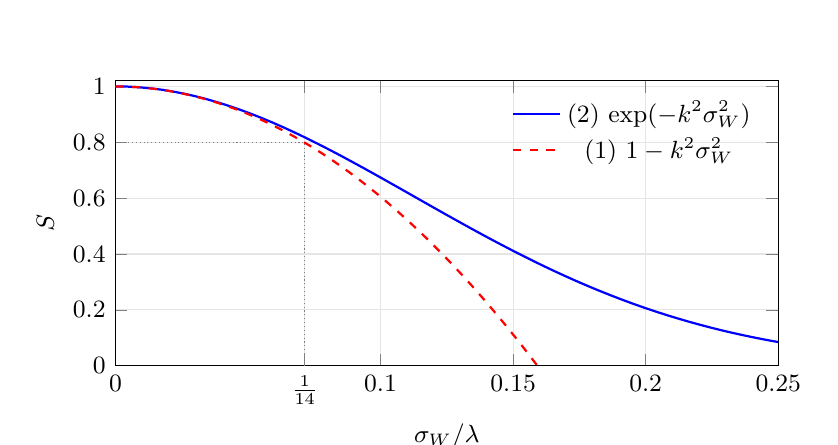
\begin{tikzpicture}
\begin{axis}[width=10cm,height=5.2cm,xmin=0,xmax=0.25,ymin=0,ymax=1.02,
  xlabel={$\sigma_W/\lambda$},ylabel={$S$},xtick={0,0.0714,0.1,0.15,0.2,0.25},
  xticklabels={0,$\frac1{14}$,0.1,0.15,0.2,0.25},ytick={0,0.2,0.4,0.6,0.8,1},
  legend style={font=\small,draw=none,fill=none,at={(0.98,0.97)},anchor=north east},
  tick label style={font=\small},label style={font=\small},grid=major,grid style={gray!20}]
\addplot[blue,thick,domain=0:0.25,samples=60]{exp(-(2*pi*x)^2)};
\addplot[red,thick,dashed,domain=0:0.159,samples=40]{1-(2*pi*x)^2};
\addplot[gray,densely dotted] coordinates {(0.0714,0)(0.0714,0.8)(0,0.8)};
\legend{(2) $\exp(-k^2\sigma_W^2)$,(1) $1-k^2\sigma_W^2$}
\end{axis}
\end{tikzpicture}

{\small 图：两种近似。$\sigma_W=\lambda/14$ 处 $S\approx0.8$；$\sigma_W$ 大于约 $\lambda/10$ 后两者明显分开。}
\end{center}

\begin{recipe}{Strehl 计算题的变式与做法}\label{rc:strehl-variants}
\begin{enumerate}
\item \textbf{给 $\sigma_W$ 求 $S$}：先化成 $\sigma_W/\lambda$（注意 nm、$\mu$m 与 $\lambda$ 单位一致），算 $x=(2\pi\sigma_W/\lambda)^2$，写 $S\approx1-x$ 和 $S\approx\ee^{-x}$ 两个值，说明哪个适用（$S$ 较大时两者接近）。
\item \textbf{给相位误差}（单位 rad，如“RMS 相位误差 0.5 rad”）：$\sigma=k\sigma_W$ 已经算好，直接 $S\approx\ee^{-\sigma^2}$。给“峰谷值 PV”时不能直接用，要先求 RMS（见 §\ref{sec:aberrms}）。
\item \textbf{给 $S$ 求容许 $\sigma_W$}：用反查式；再按像差类型换成系数容许值（如离焦 $W_{020}=\sqrt{12}\,\sigma_W$）。
\item \textbf{给具体 $W(x,y)$}：先按 §\ref{sec:aberrms} 求 $\E[W]$、$\E[W^2]$ 得 $\sigma_W$，再代 (1)/(2)。能精确积分的（如台阶）也可直接算 $|\E[\ee^{ikW}]|^2$ 对照。
\item \textbf{含倾斜}：Strehl 习惯在“实际峰值处”量，倾斜项先扣掉；若题目明确问“原点（高斯像点）处”的强度，倾斜也会使其下降，此时不扣。
\item \textbf{多种像差叠加}：Zernike 正交，$\sigma_W^2=\sum c_j^2$ 直接相加；Seidel 项之间\textbf{不}正交（如 $\rho^4$ 与 $\rho^2$），要按方差公式算交叉项（见最佳补偿套路）。
\item \textbf{非圆光瞳 / 切趾}：$\E$ 改成在实际光瞳区域上（或按振幅加权）平均，推导一字不改。
\end{enumerate}
\end{recipe}

\begin{warn}[Strehl 证明题易错]
\begin{enumerate}
\item 写出 $S=|\E[\ee^{ikW}]|^2$ 的来源：PSF 中心 = 光瞳函数积分（傅里叶变换零频），不要直接“设”出来。
\item 展开后虚部 $ik\E[W]$ 不能丢：它平方给出 $+k^2\E^2[W]$，正好与 $-k^2\E[W^2]$ 凑成方差。丢了就证不出 $\sigma_W$。
\item 写明“略去 $k^4$ 及更高阶小量”。
\item 数值：$(2\pi/14)^2=0.2014$，$1-0.2014=0.7986$；$\ee^{-0.2014}=0.8176$。
\item $k=2\pi/\lambda$，$W$ 与 $\lambda$ 同单位；$\sigma_W$ 是光程（长度），$k\sigma_W$ 才是相位（rad）。
\end{enumerate}
\end{warn}

\needspace{16\baselineskip}\section{常见像差的 RMS（单位圆光瞳，$\rho\in[0,1]$）}\label{sec:aberrms}

\begin{recipe}{给 $W(\rho,\theta)$ 求 RMS 波前误差（通用步骤）}\label{rc:rms}
\begin{enumerate}
\item \textbf{化成归一化坐标}：光瞳半径 $r_p$（直径 $a=2r_p$），$\rho=r/r_p\in[0,1]$，$\theta$ 为极角。物理坐标给的 $W(x,y)$ 先代 $x=r_p\rho\cos\theta$，$y=r_p\rho\sin\theta$。
\item \textbf{极坐标平均公式}（面元 $\rho\dd\rho\dd\theta$，单位圆面积 $\pi$）：
\[
\E[g]=\frac1\pi\int_0^{2\pi}\!\!\int_0^1 g(\rho,\theta)\,\rho\dd\rho\dd\theta
\]
\item \textbf{可分离时拆开}：$\E[\rho^n\cos^m\theta]=\E[\rho^n]\cdot\langle\cos^m\theta\rangle$，其中
\[
\E[\rho^n]=\frac1\pi\cdot2\pi\int_0^1\rho^{n+1}\dd\rho=\frac{2}{n+2},\qquad
\langle\cos\theta\rangle=0,\ \langle\cos^2\theta\rangle=\tfrac12,\ \langle\cos^3\theta\rangle=0,\ \langle\cos^4\theta\rangle=\tfrac38
\]
（$\langle\cdot\rangle=\frac1{2\pi}\int_0^{2\pi}\cdot\dd\theta$；$\sin$ 同理；$\langle\cos^2 2\theta\rangle=\frac12$。）
常用值：$\E[\rho^2]=\frac12$，$\E[\rho^4]=\frac13$，$\E[\rho^6]=\frac14$，$\E[\rho^8]=\frac15$。
\item \textbf{求 $\E[W]$ 与 $\E[W^2]$}，$\sigma_W^2=\E[W^2]-\E^2[W]$，开方。
\item \textbf{代入 Strehl}（上一节）。
\end{enumerate}
\textbf{方形/矩形光瞳}（$|x|\le L,|y|\le L$）：用 $\E[(x/L)^n]=\frac{1}{n+1}$（$n$ 偶），奇次为 0。例：$W=W_0(x/L)^2$，$\E[W]=W_0/3$，$\E[W^2]=W_0^2/5$，$\sigma_W^2=W_0^2(\frac15-\frac19)=\frac{4}{45}W_0^2$。
\end{recipe}

\begin{formula}{Seidel 像差与 RMS}\ix{离焦}\ix{球差}\ix{彗差}\ix{像散}\ix{Seidel 像差}
单位圆上平均：$\E[\rho^{n}]=\dfrac{2}{n+2}$，$\E[\cos^2\theta]=\tfrac12$，$\E[\cos^4\theta]=\tfrac38$。
\par\renewcommand{\arraystretch}{1.5}
\begin{tabular}{@{}lllll@{}}
\toprule
像差 & $W(\rho,\theta)$ & RMS（不补偿）& RMS（最佳补偿）& 补偿方式\\ \midrule
离焦 & $W_{020}\rho^2$ & $\dfrac{W_{020}}{\sqrt{12}}=0.289W_{020}$ & — & \\
球差 & $W_{040}\rho^4$ & $\dfrac{2W_{040}}{3\sqrt5}=0.298W_{040}$ & $\dfrac{W_{040}}{6\sqrt5}=0.0745W_{040}$ & 加离焦 $-W_{040}\rho^2$\\
彗差 & $W_{131}\rho^3\cos\theta$ & $\dfrac{W_{131}}{\sqrt8}=0.354W_{131}$ & $\dfrac{W_{131}}{6\sqrt2}=0.118W_{131}$ & 加倾斜 $-\tfrac23W_{131}\rho\cos\theta$\\
像散 & $W_{222}\rho^2\cos^2\theta$ & $\dfrac{W_{222}}{4}$ & $\dfrac{W_{222}}{2\sqrt6}=0.204W_{222}$ & 加离焦 $-\tfrac12W_{222}\rho^2$\\
倾斜 & $W_{111}\rho\cos\theta$ & $\dfrac{W_{111}}{2}$ & 0 & 只是像平移\\
\bottomrule
\end{tabular}

\smallskip
\textbf{逐项推导（考试可照抄对应一行）}：
\begin{itemize}
\item 离焦：$\E[W]=W_{020}\E[\rho^2]=\frac{W_{020}}2$，$\E[W^2]=W_{020}^2\E[\rho^4]=\frac{W_{020}^2}3$，$\sigma_W^2=W_{020}^2(\frac13-\frac14)=\frac{W_{020}^2}{12}$。
\item 球差：$\E[\rho^4]=\frac13$，$\E[\rho^8]=\frac15$，$\sigma_W^2=W_{040}^2(\frac15-\frac19)=\frac{4W_{040}^2}{45}$，$\sigma_W=\frac{2W_{040}}{3\sqrt5}$。
\item 彗差：$\E[\rho^3\cos\theta]=\frac25\cdot0=0$，$\E[\rho^6\cos^2\theta]=\frac14\cdot\frac12=\frac18$，$\sigma_W=\frac{W_{131}}{\sqrt8}$。
\item 像散：$\E[\rho^2\cos^2\theta]=\frac12\cdot\frac12=\frac14$，$\E[\rho^4\cos^4\theta]=\frac13\cdot\frac38=\frac18$，$\sigma_W^2=W_{222}^2(\frac18-\frac1{16})=\frac{W_{222}^2}{16}$。
\item 倾斜：$\E[W]=0$，$\E[\rho^2\cos^2\theta]=\frac14$，$\sigma_W=\frac{W_{111}}2$。
\end{itemize}

\textbf{瑞利 $\lambda/4$ 判据}：离焦 $W_{020}=\lambda/4$ $\Rightarrow\sigma_W=\frac{\lambda}{4\sqrt{12}}=\frac{\lambda}{13.9}$，正好就是 $\lambda/14$，$S\approx0.8$。两个判据一致。
\end{formula}

\begin{recipe}{最佳补偿（平衡像差）= 求方差最小 = 线性回归}\label{rc:balance}\ix{像差平衡}
\textbf{题型}：“加入适量离焦（移动像面）/ 倾斜（换参考点）使 RMS 最小，求补偿量与最小 RMS”。课件：适量离焦可补偿球差 [F3-p99, p117]。

\textbf{一般公式}：$W=W_0\,[f+c\,g]$（$f$ 原像差形状，$g$ 补偿项形状，$c$ 待定）。
\[
\frac{\sigma_W^2}{W_0^2}=\mathrm{Var}f+2c\,\mathrm{Cov}(f,g)+c^2\,\mathrm{Var}g
\]
\[
\frac{\dd}{\dd c}=0\ \Rightarrow\ \boxed{c^*=-\frac{\mathrm{Cov}(f,g)}{\mathrm{Var}\,g}},\qquad
\sigma_{\min}^2=W_0^2\Big[\mathrm{Var}f-\frac{\mathrm{Cov}^2(f,g)}{\mathrm{Var}\,g}\Big]
\]
其中 $\mathrm{Var}f=\E[f^2]-\E^2[f]$，$\mathrm{Cov}(f,g)=\E[fg]-\E[f]\E[g]$。

\textbf{例：球差 + 离焦}（$f=\rho^4$，$g=\rho^2$）：
$\mathrm{Var}f=\frac15-\frac19=\frac4{45}$，$\mathrm{Var}g=\frac13-\frac14=\frac1{12}$，
$\mathrm{Cov}=\E[\rho^6]-\E[\rho^4]\E[\rho^2]=\frac14-\frac16=\frac1{12}$。\\
$c^*=-\frac{1/12}{1/12}=-1$（加离焦 $-W_{040}\rho^2$），
$\sigma_{\min}^2=W_{040}^2\big(\frac4{45}-\frac{1}{12}\big)=\frac{W_{040}^2}{180}$，$\sigma_{\min}=\frac{W_{040}}{6\sqrt5}=0.0745W_{040}$（降到原来的 1/4）。

\textbf{彗差 + 倾斜}（$f=\rho^3\cos\theta$，$g=\rho\cos\theta$）：$\mathrm{Var}f=\frac18$，$\mathrm{Var}g=\frac14$，$\mathrm{Cov}=\E[\rho^4\cos^2\theta]=\frac16$；
$c^*=-\frac23$，$\sigma_{\min}^2=W_{131}^2(\frac18-\frac19)=\frac{W_{131}^2}{72}$。

\textbf{像散 + 离焦}（$f=\rho^2\cos^2\theta$，$g=\rho^2$）：$\mathrm{Var}f=\frac1{16}$，$\mathrm{Var}g=\frac1{12}$，$\mathrm{Cov}=\frac16-\frac14\cdot\frac12=\frac1{24}$；
$c^*=-\frac12$（像面放在两条焦线中间，“最小弥散圆”），$\sigma_{\min}^2=W_{222}^2(\frac1{16}-\frac1{48})=\frac{W_{222}^2}{24}$。

\textbf{物理意义}：加离焦 $W_{020}$ = 把观察面沿轴移动 $\Delta z=2W_{020}/\mathrm{NA}'^2$（见下框）；加倾斜 = 把参考点横移，即在实际峰值处量 Strehl。
Zernike 语言：最佳补偿后的 RMS 就是该像差最高阶 Zernike 项的系数（见第 \pageref{sec:zernike} 页）。
\end{recipe}

\begin{exam}{数值例：同一像差，补偿前后的 Strehl（$\lambda$ 为单位）}\label{ex:balance-num}
\par\renewcommand{\arraystretch}{1.3}
\begin{tabular}{@{}lccccc@{}}
\toprule
像差（系数） & 补偿 & $\sigma_W/\lambda$ & $x=(2\pi\sigma_W/\lambda)^2$ & (1) $1-x$ & (2) $\ee^{-x}$\\ \midrule
球差 $W_{040}=0.5\lambda$ & 无 & $0.298\times0.5=0.149$ & 0.877 & 0.12 & 0.42\\
 & 加离焦 $-0.5\lambda\rho^2$ & $0.0745\times0.5=0.0373$ & 0.055 & 0.945 & 0.947\\
彗差 $W_{131}=0.3\lambda$ & 无 & 0.106 & 0.445 & 0.555 & 0.641\\
 & 加倾斜 & 0.0354 & 0.050 & 0.951 & 0.952\\
像散 $W_{222}=0.4\lambda$ & 无 & 0.100 & 0.395 & 0.605 & 0.674\\
 & 加离焦 $-0.2\lambda\rho^2$ & 0.0816 & 0.263 & 0.737 & 0.769\\
\bottomrule
\end{tabular}\par\smallskip
答题写法（以球差为例）：“$\sigma_W=\frac{2W_{040}}{3\sqrt5}=0.149\lambda$，$S\approx\exp[-(2\pi\times0.149)^2]=\ee^{-0.877}=0.42$；
加入离焦 $-W_{040}\rho^2$ 后 $\sigma_W=\frac{W_{040}}{6\sqrt5}=0.0373\lambda$，$S\approx1-0.055=0.945$，像质显著改善。”
\end{exam}

\needspace{10\baselineskip}
\begin{formula}{离焦量的四种表示与焦深}\ix{焦深}\ix{离焦!与轴向位移}\label{sec:defocus-units}
\textbf{(a) 课件写法 [F3-p51–52]}：传感器在 $l'$，实际会聚点在 $l'+\Delta$，出瞳直径 $a$：
\[
W(\xi,\eta)=\Big(\frac1{l'}-\frac1{l'+\Delta}\Big)\frac{\xi^2+\eta^2}{2}\approx b\,\frac{\xi^2+\eta^2}{2},\quad b=\frac{\Delta}{l'^2};\qquad
W_{\max}=b\,\frac{a^2}{8}\ \ (\text{边缘 }\xi^2+\eta^2=a^2/4)
\]
推导：理想出瞳复振幅 $\exp[-ik\frac{r^2}{2l'}]$，实际 $\exp[-ik\frac{r^2}{2(l'+\Delta)}]$，两者之比 $=\ee^{ikW}$。

\textbf{(b) 归一化写法}：令 $\rho=r/(a/2)$，$W=\frac{b a^2}{8}\rho^2$，所以 $\boxed{W_{020}=W_{\max}=\dfrac{\Delta a^2}{8l'^2}}$。

\textbf{(c) 用 NA 或 $F/\#$}：$\mathrm{NA}'\approx\frac{a}{2l'}$，$F/\#\approx\frac{l'}{a}$，
\[
W_{020}=\frac{\Delta}{2}\,\mathrm{NA}'^2=\frac{\Delta}{8(F/\#)^2}\qquad\Longleftrightarrow\qquad\Delta=\frac{2W_{020}}{\mathrm{NA}'^2}=8(F/\#)^2W_{020}
\]
\textbf{(d) 用屈光度}（视光学）：屈光误差 $\Delta\Phi$（单位 D），瞳孔半径 $r_p$：$W_{020}=\dfrac{\Delta\Phi\,r_p^2}{2}$（薄透镜相位 $-k\Phi r^2/2$）。

\textbf{焦深}：令 $W_{020}\le\lambda/4$（等价于 $\sigma_W\le\lambda/14$，$S\ge0.8$）：
\[
\boxed{|\Delta|\le\dfrac{\lambda}{2\,\mathrm{NA}'^2}=2\lambda(F/\#)^2}
\]
小瞳孔（NA 小）焦深大，$\propto D^{-2}$ [VO-p95]。
另一个临界：$W_{\max}=\lambda/2$（$\Delta=4\lambda(F/\#)^2$）时离焦 OTF 开始出现负值、条纹黑白反转（第 \ref{ch:imaging} 章离焦 OTF）。
\end{formula}

\begin{exam}{数值例：离焦（课件参数 $a=2$ mm，$l'=10$ mm，$\lambda=0.55\,\mu$m）}\label{ex:defocus-strehl}
$F/\#=l'/a=5$，焦深 $|\Delta|\le2\lambda(F/\#)^2=2\times0.55\times25=27.5\,\mu$m。\\
若传感器偏离 $\Delta=50\,\mu$m：$W_{020}=\dfrac{\Delta a^2}{8l'^2}=\dfrac{50\times(2/10)^2}{8}=0.25\,\mu\text{m}=0.455\lambda$；
$\sigma_W=\dfrac{W_{020}}{\sqrt{12}}=0.131\lambda$；$x=(2\pi\times0.131)^2=0.680$；
$S\approx1-0.68=0.32$（(1) 已在边缘），$S\approx\ee^{-0.68}=0.51$。
结论：超出焦深（$W_{020}>\lambda/4$），且接近 $\lambda/2$ 的反转临界。\\
\textbf{视光学版}：瞳孔 6 mm（$r_p=3$ mm），离焦 0.5 D：$W_{020}=\frac{0.5\times(3\times10^{-3})^2}{2}$ m $=2.25\,\mu$m $=4.1\lambda$，$\sigma_W=0.65\,\mu$m，$S\approx0$（远超近似范围，像质由几何弥散斑主导）。
同样 0.5 D 在 2 mm 瞳孔：$W_{020}=0.25\,\mu$m，与上例同量级——小瞳孔焦深大。
\end{exam}

\needspace{10\baselineskip}
\begin{formula}{Zernike 多项式（ANSI 编号，RMS 归一化）}\ix{Zernike 多项式}\label{sec:zernike}
\textbf{为什么用 Zernike} [F3-p94–98]：在单位圆上正交（权重 $\rho\dd\rho\dd\theta$），分离变量 $Z=R(\rho)\Theta(\theta)$，角向用三角函数；每项对应一种经典像差。
\textbf{归一化}：每项（除 piston）在单位圆上 RMS $=1$，均值为 0。所以
\[
W=\sum_j c_jZ_j\ \Rightarrow\ \boxed{\sigma_W^2=\sum_{j\ge1}c_j^2}\quad(\text{扣去 piston } c_0\text{；若题目说扣倾斜，再去掉 }c_1,c_2)
\]
\par\renewcommand{\arraystretch}{1.3}
\begin{tabular}{@{}cclll@{}}
\toprule
$j$ & $Z_n^m$ & 多项式 & 名称 & 效果\\ \midrule
0 & $Z_0^0$ & $1$ & piston & 不影响成像\\
1, 2 & $Z_1^{-1},Z_1^{1}$ & $2\rho\sin\theta,\ 2\rho\cos\theta$ & tilt & 像平移\\
3, 5 & $Z_2^{-2},Z_2^{2}$ & $\sqrt6\rho^2\sin2\theta,\ \sqrt6\rho^2\cos2\theta$ & astigmatism & 像散（柱镜）\\
4 & $Z_2^0$ & $\sqrt3(2\rho^2-1)$ & defocus & 离焦\\
7, 8 & $Z_3^{-1},Z_3^{1}$ & $\sqrt8(3\rho^3-2\rho)\sin\theta,\ \cos\theta$ & coma & 彗差\\
6, 9 & $Z_3^{\mp3}$ & $\sqrt8\rho^3\sin3\theta,\ \cos3\theta$ & trefoil & 三叶\\
12 & $Z_4^0$ & $\sqrt5(6\rho^4-6\rho^2+1)$ & spherical & 球差\\
\bottomrule
\end{tabular}

\smallskip
编号 $j=\dfrac{n(n+2)+m}{2}$；$m<0$ 对应 $\sin$，$m>0$ 对应 $\cos$；归一化系数：$m=0$ 为 $\sqrt{n+1}$，$m\ne0$ 为 $\sqrt{2(n+1)}$ [F3-p98, p103]。
PSF 形状的对称性与角向阶 $|m|$ 对应（离焦/球差圆对称，彗差彗星形，三叶三角形）[F3-p118]。
眼科：低阶（离焦+像散）可用球柱镜矫正，约占 85–90\%；其余为高阶像差 HOA [VO-p94,95]。
\end{formula}

\begin{recipe}{Zernike 题的三种做法}\label{rc:zernike}
\begin{enumerate}
\item \textbf{给系数求 RMS / Strehl}：$\sigma_W=\sqrt{\sum c_j^2}$（单位同系数），再代 Strehl。
\item \textbf{Seidel 换 Zernike}：用 $\rho^2=\frac12+\frac{1}{2\sqrt3}Z_4$，$\rho^4=\frac13+\frac{1}{2\sqrt3}Z_4+\frac1{6\sqrt5}Z_{12}$。\\
验证：$\frac{Z_{12}}{6\sqrt5}=\rho^4-\rho^2+\frac16$，$\frac{Z_4}{2\sqrt3}=\rho^2-\frac12$，相加 $=\rho^4-\frac13$。\\
所以 $W_{040}\rho^4$：$c_4=\frac{W_{040}}{2\sqrt3}$，$c_{12}=\frac{W_{040}}{6\sqrt5}$；$\sigma_W^2=W_{040}^2(\frac1{12}+\frac1{180})=\frac{4}{45}W_{040}^2$，与 Seidel 表一致；
去掉 $c_4$（加离焦补偿）剩 $c_{12}=0.0745W_{040}$，就是“最佳补偿 RMS”。离焦 $W_{020}\rho^2$ 只有 $c_4=\frac{W_{020}}{2\sqrt3}=\frac{W_{020}}{\sqrt{12}}$。
\item \textbf{离焦系数 $\leftrightarrow$ 屈光度}：$W_{020}=\sqrt{12}\,c_4$，$\Delta\Phi=\dfrac{2W_{020}}{r_p^2}=\dfrac{4\sqrt3\,c_4}{r_p^2}$（$r_p$ 瞳孔半径）。
\end{enumerate}
\textbf{数值例}（瞳孔 6 mm，$\lambda=0.55\,\mu$m）：$c_4=0.2$，$c_7=0.05$，$c_{12}=0.1$（$\mu$m）。
$\sigma_W=\sqrt{0.04+0.0025+0.01}=0.229\,\mu$m $=0.417\lambda$，$x=6.85$，$S\approx\ee^{-6.85}\approx0.001$（像质很差，已出近似范围）。
配镜矫正离焦（$c_4\to0$）后 $\sigma_W=0.112\,\mu$m $=0.203\lambda$，$S\approx\ee^{-1.63}=0.20$。
对应屈光误差 $\Delta\Phi=\frac{4\sqrt3\times0.2\times10^{-6}}{(3\times10^{-3})^2}=0.154$ D。
\end{recipe}

\needspace{8\baselineskip}\section{波像差与光线像差、波前测量 [F3-p94–126]}\label{sec:rayaberr}
\begin{formula}{波像差 $\to$ 光线像差}\ix{光线像差}\ix{Shack-Hartmann}\ix{点列图}
\textbf{原理}：光线是波前的法线 [F3-p95]。实际波前相对参考球面在 $x$ 方向的斜率 $\partial W/\partial x$ = 实际光线与理想光线的夹角（小角）。
光线再走参考球面半径 $R$（出瞳到高斯像点，$R\gg W$）到达像面，横向偏离 $\approx R\times$角度：
\[
\boxed{T_X\approx-R\frac{\partial W}{\partial x},\qquad T_Y\approx-R\frac{\partial W}{\partial y}},\qquad \vec T=-R\nabla W
\]
（负号取决于 $W$ 的符号约定，大小 $|\vec T|=R|\nabla W|$ 不变。）\\
\textbf{套用步骤}：写出物理坐标下的 $W(x,y)$ → 求偏导 → 乘 $-R$ → 在光瞳边缘取最大值得弥散斑半径。
\begin{itemize}
\item \textbf{倾斜} $W=\alpha x$：$T_X=-R\alpha$，所有光线同样偏移（像平移，PSF 形状不变）。
\item \textbf{离焦} $W=W_{020}r^2/r_p^2$：$T_X=-2RW_{020}x/r_p^2$，与瞳孔坐标成线性 $\Rightarrow$ 均匀弥散圆，半径 $\dfrac{2RW_{020}}{r_p}$。\\
\textbf{核对课件}：$W=b\frac{r^2}{2}$，$b=\frac{\Delta}{l'^2}$，$R=l'$，边缘 $r=\frac a2$：$|T|=l'\cdot b\cdot\frac a2=\frac{a\Delta}{2l'}$，弥散圆直径 $\frac{a\Delta}{l'}$，与相似三角形 $d\approx a\Delta/l'$ 一致 [F3-p56]。
\item \textbf{球差} $W=W_{040}r^4/r_p^4$：$|T|=\dfrac{4RW_{040}}{r_p}\rho^3$，边缘光线偏得最多，中心光线几乎不偏：点列图中心密、外围有晕；加适量离焦可平衡（RMS 降到 1/4）。离焦与球差的点列图不同：离焦是均匀圆盘（$T\propto\rho$），球差中心亮外围晕（$T\propto\rho^3$）[F3-p110–117]。
\item \textbf{严重离焦}时 PSF 趋近几何弥散圆，其 OTF $=\dfrac{2J_1(\pi d\rho)}{\pi d\rho}$，第一零点 $\rho=1.22/d$ [F3-p56]。
\end{itemize}
像差类型：球差、彗差、像散、场曲、畸变（单色五种），轴向色差、倍率色差 [F3-p99–102]。
\end{formula}

\begin{formula}{Shack-Hartmann 波前传感器 [F3-p123–126]}\ix{波前测量}
微透镜阵列（焦距 $f_{\text{ml}}$）把波前切成小块，每块在自己焦面上成一个焦斑。
平面波前：焦斑落在各自光轴上（规则点阵）；畸变波前：每块的局部倾斜使焦斑偏移
\[
\Delta x_i=f_{\text{ml}}\left.\frac{\partial W}{\partial x}\right|_i,\qquad \Delta y_i=f_{\text{ml}}\left.\frac{\partial W}{\partial y}\right|_i
\]
测出所有斜率 → 积分或拟合 Zernike 系数 → 得 $W$ → 求 RMS、Strehl、屈光度。
（与上一框同一原理：局部斜率 × 传播距离 = 横向偏移，这里传播距离是 $f_{\text{ml}}$。）\\
\textbf{数值例}：$f_{\text{ml}}=6$ mm，瞳孔半径 $r_p=3$ mm；测得焦斑偏移与位置成正比，边缘 $x=3$ mm 处偏 12 $\mu$m。
线性 $\Rightarrow$ 纯离焦：$\frac{\partial W}{\partial x}=\frac{2W_{020}x}{r_p^2}$；边缘斜率 $=\frac{12\,\mu\text{m}}{6\text{ mm}}=2\times10^{-3}$ $\Rightarrow$ $\frac{2W_{020}}{r_p}=2\times10^{-3}$，$W_{020}=3\,\mu$m；
$\sigma_W=\frac{3}{\sqrt{12}}=0.87\,\mu$m；屈光误差 $\Delta\Phi=\frac{2W_{020}}{r_p^2}=\frac{6\times10^{-6}}{9\times10^{-6}}=0.67$ D。
\end{formula}

\begin{exam}{人眼高阶像差的 Strehl 比}
瞳孔 6 mm，HOA RMS $=0.3\,\mu$m，$\lambda=0.55\,\mu$m：
$k\sigma_W=\frac{2\pi\times0.3}{0.55}=3.43$ rad，$S\approx\ee^{-11.7}\approx0$（远不满足近似，像质很差）。
瞳孔 3 mm，HOA RMS $=0.07\,\mu$m：$k\sigma_W=0.80$，$S\approx\ee^{-0.64}=0.53$。
瞳孔从 3 mm 缩到更小时像差下降，但衍射斑 $\propto1/D$ 变大，所以约 3 mm 最佳。
\end{exam}

\begin{warn}[本章计算题总检查]
\begin{enumerate}
\item 单位：$W$、$\sigma_W$、$\lambda$ 统一成同一单位（$\mu$m 或 $\lambda$）；屈光度用米。
\item 光瞳“直径 $a$”与“半径 $r_p$”别混：课件离焦 $W_{\max}=ba^2/8$ 用的是直径。
\item 峰谷值（PV，如 $W_{020}$、$W_{\max}$）$\ne$ RMS：离焦 RMS $=$ PV$/\sqrt{12}$。
\item Seidel 项不正交，叠加时有交叉项；Zernike 项正交，平方和即可。
\item Strehl 近似只在 $S$ 较大时可信，$S$ 很小时只说“像质很差、需用几何光学估计”。
\end{enumerate}
\end{warn}

\chapter{视光学}\label{ch:visual}

\begin{idea}[视光学的考法]
视光学按“计算 + 画图”准备：
\textbf{屈光度加减}（眼、眼镜、透镜组）、\textbf{三种放大率}、\textbf{孔径光阑 / 入瞳 / 出瞳的判断与作图}、
\textbf{角分辨率与 CPD / 视力换算}、\textbf{CSF 与 MTF}、\textbf{gamma 计算}、\textbf{像素采样的频谱}。
其中后几项和傅里叶光学直接相连（人眼 = 一个成像系统 + 一个采样器 + 一个低通滤波器）。
\end{idea}

\begin{warn}[{本章的符号约定 [VO-p30,31,35,36]}]
\textbf{高斯约定}：物距 $l$、像距 $l'$ 都取\textbf{正值表示实物、实像}（物在透镜左边、像在透镜右边）；虚像 $l'<0$（像和物在同一侧），虚物 $l<0$。
会聚透镜 $f>0$，发散透镜 $f<0$。屈光度（光焦度）$\Phi=1/f$，\textbf{$f$ 必须用米}，单位 D $=$ m$^{-1}$。
空气中写 $\Phi_{\text{物}}=1/l$、$\Phi_{\text{像}}=1/l'$。物方空气、像方折射率 $n'$ 时，改写为 $\Phi_{\text{像}}=n'/l'$ [VO-p30]。
课件 p31、p35 的图用放大率大小 $|\beta|=|l'/l|$、$|\gamma|=1/|\beta|$；本章用带符号的像高和光线倾角，倒像 $\beta<0$。入射、出射倾角均以向右光轴为基准，向上偏转为正；轴向坐标 $Z_o,Z_i$ 也向右为正，位移比 $\alpha=\dd Z_i/\dd Z_o$ [VO-p36]。
\end{warn}

\needspace{8\baselineskip}\section{薄透镜、放大率、基点}
\begin{formula}{高斯公式与三种放大率（课件约定：$l,l'$ 取正 = 实物、实像）}\ix{高斯公式}\ix{横向放大率}\ix{角放大率}\ix{纵向放大率}
\[
\frac1l+\frac1{l'}=\frac1f\qquad\Longleftrightarrow\qquad\Phi_{\text{物}}+\Phi_{\text{像}}=\Phi\quad(\Phi=1/\text{距离，单位 D=m}^{-1})
\]
空气薄透镜的牛顿形式：$(l-f)(l'-f)=f^2$，两侧焦距均用上式的 $f$。
\par\renewcommand{\arraystretch}{1.5}
\begin{tabular}{@{}lll@{}}
\toprule
横向（垂轴）放大率 & $\beta=\dfrac{y'}{y}=-\dfrac{l'}{l}$ & [VO-p30,31]\\
角放大率（有向角） & $\gamma=\dfrac{\tan u'}{\tan u}=-\dfrac{l}{l'}=\dfrac1\beta$ & [VO-p35]\\
纵向（轴向）放大率 & $\alpha=\dfrac{\dd Z_i}{\dd Z_o}=\beta^2$ & [VO-p36]\\
关系（同一介质） & $\beta=\alpha\gamma$ & [VO-p37]\\
\bottomrule
\end{tabular}

\smallskip
物像方折射率为 $n,n'$ 时，傍轴关系为 $\alpha=(n'/n)\beta^2$、$\gamma=(n/n')/\beta$，仍有 $\beta=\alpha\gamma$。
同一介质的纵向放大率 $=\beta^2$ 正是 4f 偏离补偿题 $x_2=M^2x_1$ 的几何解释（§\ref{sec:4foffset}）。
\end{formula}

\subsection{题型：单个薄透镜成像（求像的位置、大小、正倒、虚实）}\label{sec:lensimg}
\textbf{【题型】}“物高 $y$、物距 $l$，焦距 $f$（或屈光度 $\Phi$）的透镜，求像距、放大率、像的性质”；或反过来“要在某处成像，透镜需要多少度”。

\textbf{【完整推导】}（每一步都可以照抄）
\begin{enumerate}
\item 统一单位：距离全部换成\textbf{米}，才能和 D 相加减。依据：$\Phi=1/f[\text{m}]$。
\item 写聚散度：$\Phi_{\text{物}}=\dfrac1l$。依据：高斯公式左边第一项。
\item 求像方聚散度：$\Phi_{\text{像}}=\Phi-\Phi_{\text{物}}$。依据：$\Phi_{\text{物}}+\Phi_{\text{像}}=\Phi$（成像只是\textbf{加减法} [VO-p49]）。
\item 像距 $l'=1/\Phi_{\text{像}}$。$l'>0$：实像，在透镜右侧；$l'<0$：虚像，在透镜左侧（与物同侧）距离 $|l'|$。
\item 横向放大率 $\beta=-\dfrac{l'}{l}$（带符号）：$\beta<0$ 倒立，$\beta>0$ 正立；$|\beta|>1$ 放大。依据：过光心的光线不偏折，两个相似三角形 $\dfrac{|y'|}{|y|}=\dfrac{|l'|}{|l|}$ [VO-p31]。
\item 像高 $y'=\beta y$；角放大率 $\gamma=1/\beta$，纵向放大率 $\alpha=\beta^2$（永远为正：物沿轴往右移，像也往右移）。
\end{enumerate}

\textbf{纵向放大率的推导 [VO-p30,36]}：固定透镜位置，$l$ 向左量、$l'$ 向右量，故 $\dd l=-\dd Z_o$、$\dd l'=\dd Z_i$。对 $1/l+1/l'=1/f$ 微分，得 $\dd l'/\dd l=-l'^2/l^2$，因此
\[
\alpha=\frac{\dd Z_i}{\dd Z_o}=-\frac{\dd l'}{\dd l}=\frac{l'^2}{l^2}=\beta^2.
\]
一般介质下由 $n/l+n'/l'=\Phi$、$\beta=-nl'/(n'l)$ 同样得到 $\alpha=(n'/n)\beta^2$。

\begin{exam}{答题模板：薄透镜成像}
\textbf{解}：取高斯约定（实物、实像距离为正）。已知 $l=\underline{\quad}$ m，$\Phi=1/f=\underline{\quad}$ D。\\
由 $\Phi_{\text{物}}+\Phi_{\text{像}}=\Phi$：$\Phi_{\text{像}}=\Phi-\dfrac1l=\underline{\quad}$ D，故 $l'=\dfrac1{\Phi_{\text{像}}}=\underline{\quad}$ m（$>0$ 实像在透镜后 / $<0$ 虚像在透镜前）。\\
横向放大率 $\beta=-\dfrac{l'}{l}=\underline{\quad}$，像高 $y'=\beta y=\underline{\quad}$（倒立/正立，放大/缩小）。
\end{exam}

\begin{exam}{数值例：$f=+10$ cm 的透镜，物高 2 cm}
(a) $l=30$ cm：$\Phi=10$ D，$\Phi_{\text{物}}=3.33$ D，$\Phi_{\text{像}}=6.67$ D，$l'=15$ cm（实像）；$\beta=-15/30=-0.5$，像高 $-1$ cm（倒立缩小）。\\
(b) $l=5$ cm（物在焦内，放大镜）：$\Phi_{\text{物}}=20$ D，$\Phi_{\text{像}}=10-20=-10$ D，$l'=-10$ cm（虚像在透镜前 10 cm）；$\beta=-(-10)/5=+2$，像高 $+4$ cm（正立放大虚像）。\\
(c) 换成 $f=-10$ cm（$-10$ D），$l=30$ cm：$\Phi_{\text{像}}=-10-3.33=-13.33$ D，$l'=-7.5$ cm（虚像）；$\beta=+0.25$（正立缩小）。发散透镜对实物永远成正立缩小虚像。
\end{exam}

\textbf{【适配/变式】}
\begin{itemize}
\item \textbf{物在无穷远}：$\Phi_{\text{物}}=0\Rightarrow l'=f$（像在焦面）。像大小用角度算：$y'=f\tan\theta$（$\theta$ 为物对透镜的张角）。
\item \textbf{物在焦点上}：$\Phi_{\text{像}}=0\Rightarrow l'=\infty$，出射平行光（放大镜、准直）。
\item \textbf{虚物}（会聚光射来，若无透镜会聚到透镜后 $s$ 处）：$l=-s$，$\Phi_{\text{物}}=-1/s$，其余照算。
\item \textbf{反求透镜}：要物距 $l$ 成像到 $l'$：$\Phi=\dfrac1l+\dfrac1{l'}$（虚像代负值）。这就是配眼镜的计算（\pageref{sec:correct}套路）。
\item \textbf{物像方折射率不同}（如眼内为 $n'$）：$\dfrac{1}{l}+\dfrac{n'}{l'}=\Phi$，像方聚散度写成 $n'/l'$；放大率 $\beta=-\dfrac{l'}{n'l}$。
\end{itemize}

\begin{formula}{透镜组与屈光度}\ix{屈光度}\ix{透镜组}\ix{光焦度}
\[
\Phi=\Phi_1+\Phi_2-d\,\Phi_1\Phi_2,\qquad f=\frac{f_1f_2}{f_1+f_2-d}
\]
密接（$d=0$）：$\Phi=\Phi_1+\Phi_2$。凸透镜 $f=20$ cm $\Rightarrow+5$ D；凹透镜 $f=-20$ cm $\Rightarrow-5$ D。\\
眼镜“度数” $=$ 屈光度 $\times100$（$-3$ D $=$ 300 度近视）。
\end{formula}

\subsection{题型：两片透镜（透镜组）——等效光焦度或逐次成像}\label{sec:lenscombo}
\textbf{【推导】组合光焦度公式}（跟踪一条平行于轴、高度 $h_1$ 的光线）：
\begin{enumerate}
\item 过透镜 1 后光线的倾角（向轴偏折）$u_1=h_1\Phi_1$。依据：薄透镜把高度 $h$ 的平行光偏折 $h/f$，使其射向焦点。
\item 走过间距 $d$ 后高度 $h_2=h_1-d\,u_1=h_1(1-d\Phi_1)$。
\item 过透镜 2 后倾角 $u_2=u_1+h_2\Phi_2=h_1[\Phi_1+\Phi_2-d\Phi_1\Phi_2]$。依据：薄透镜对任意入射光线的偏折量都是 $h\Phi$。
\item 等效光焦度定义为“入射平行光高度 $h_1$ $\to$ 出射倾角”：$\Phi=u_2/h_1=\Phi_1+\Phi_2-d\Phi_1\Phi_2$。
\item 后截距（透镜 2 到像方焦点）$\mathrm{BFL}=h_2/u_2=\dfrac{1-d\Phi_1}{\Phi}$；等效焦距 $f=1/\Phi$ 从像方主面量起，主面 H$'$ 在透镜 2 左边 $f-\mathrm{BFL}=\dfrac{d\Phi_1}{\Phi}$ 处。
\end{enumerate}

\begin{recipe}{逐次成像法（任何多透镜题都适用，最不容易错）}
\begin{enumerate}
\item 第 1 片：照 §\ref{sec:lensimg} 求 $l_1'$、$\beta_1$。
\item 第 1 片的像就是第 2 片的物：$l_2=d-l_1'$。$l_2>0$ 实物（像在第 2 片左边）；$l_2<0$ 虚物（$l_1'>d$，光还没会聚就进了第 2 片）。
\item 第 2 片：再求 $l_2'$、$\beta_2$。
\item 总放大率 $\beta=\beta_1\beta_2$，总像高 $y'=\beta y$。
\end{enumerate}
\end{recipe}

\begin{exam}{数值例：$f_1=+10$ cm、$f_2=+20$ cm，相距 $d=15$ cm，物在第 1 片前 30 cm}
第 1 片：$l_1'=15$ cm，$\beta_1=-0.5$。第 2 片：$l_2=15-15=0$？物恰在第 2 片上 $\Rightarrow$ 像也在第 2 片上，$\beta_2=1$（贴着透镜的物不被它改变）。\\
改 $d=25$ cm：$l_2=25-15=10$ cm，$\Phi_{\text{像}}=5-10=-5$ D，$l_2'=-20$ cm（虚像在第 2 片前 20 cm），$\beta_2=-(-20)/10=+2$；总 $\beta=-1$（倒立等大虚像）。\\
等效光焦度（$d=25$ cm）：$\Phi=10+5-0.25\times10\times5=2.5$ D，$f=40$ cm。
\end{exam}

\begin{formula}{基点：焦点 F/F$'$、主点 H/H$'$、节点 N/N$'$}\ix{基点}\ix{主点}\ix{节点}\ix{有效焦距 EFL}
\begin{itemize}
\item 主面：横向放大率 $+1$ 的一对共轭面；光线在 H 面上的高度 = 从 H$'$ 面出射的高度。\textbf{EFL 从主面量起}，不是从顶点。
\item 节点：射向 N 的光线从 N$'$ 以\textbf{相同方向}射出（角放大率 $+1$）。物像方折射率相同时 N$\equiv$H，N$'$$\equiv$H$'$。
\item 焦点和主点的位置见 [VO-p39,41]。此处用有向焦距 $f_o=\overline{HF}$、$f_i=\overline{H'F'}$（向右为正）：$f_o=-n/\Phi$、$f_i=n'/\Phi$，所以 $-f_i/f_o=n'/n$。节点满足 $\overline{HN}=f_o+f_i$ [VO-p44,45]。空气会聚系统中 $f_o=-f$、$f_i=f$，与前面高斯公式的 $f>0$ 对应。
\item 作图三条线：平行轴入射 $\to$ 在 H$'$ 折向 F$'$；过 F 入射 $\to$ 自 H$'$ 平行出射；射向 N $\to$ 自 N$'$ 平行出射。
\end{itemize}
\end{formula}

\begin{recipe}{画图题：已知基点，作出某物点的像 [VO-p41,44]}\ix{画图题!基点作图}
\begin{enumerate}
\item 画光轴，按比例标出 F、H、H$'$、F$'$（有节点就标 N、N$'$）。H、H$'$ 之间光线\textbf{水平平移}（不画实际折射）。
\item 光线①：物点平行于轴射到 \textbf{H$'$ 面}（高度不变穿过 H、H$'$），从 H$'$ 折向 F$'$。
\item 光线②：物点经 F 射到 \textbf{H 面}，从 H$'$ 平行于轴射出（高度与在 H 面上相同）。
\item 光线③（可选，校核）：物点射向 N，从 N$'$ 射出，方向与入射\textbf{平行}。
\item 两条出射光线交点即像点；若出射光线发散，反向延长（虚线）交于虚像。标出像高与像距（从 H$'$ 量）。
\end{enumerate}
\end{recipe}

\begin{center}
\begin{tikzpicture}[x=0.55cm,y=0.55cm,>=Stealth,font=\scriptsize]
\draw[->] (-8,0)--(10,0) node[right]{光轴};
\draw[thick,gray] (0,-2.2)--(0,3) node[above]{H}; \draw[thick,gray] (1,-2.2)--(1,3) node[above]{H$'$};
\fill (-3,0) circle (2pt) node[below]{F}; \fill (4,0) circle (2pt) node[below]{F$'$};
\draw[->,very thick,blue] (-6,0)--(-6,1.5) node[above]{物 $y$};
\draw[red,thick] (-6,1.5)--(0,1.5)--(1,1.5)--(9,-2.5); \node[red] at (-3,1.85){①};
\draw[red!60!black,thick,dashed] (-6,1.5)--(-3,0)--(0,-1.5)--(1,-1.5)--(9,-1.5); \node[red!60!black] at (-4.8,1.25){②};
\draw[->,very thick,blue] (7,0)--(7,-1.5) node[below]{像 $y'$};
\draw[<->] (0,-2.6)--(-3,-2.6) node[midway,below]{$|f_o|$}; \draw[<->] (1,-2.6)--(4,-2.6) node[midway,below]{$f_i$};
\end{tikzpicture}

{\scriptsize 例图：$f_o=-3$，$f_i=3$，物距 6（从 H 量），像距 6（从 H$'$ 量），$\beta=-1$。}
\end{center}

\needspace{8\baselineskip}\section{人眼的光学参数}
\begin{formula}{Gullstrand 模型眼数据（从角膜顶点量，mm）}\ix{人眼!参数}\ix{模型眼}
\par\renewcommand{\arraystretch}{1.3}
\begin{tabular}{@{}ll|ll@{}}
\toprule
物方焦点 F & $-15.707$ & 有向物方焦距 $f_o$ & $-17.055$\\
物方主点 H & $1.348$ & 有向像方焦距 $f_i$ & $+22.785$\\
像方主点 H$'$ & $1.602$ & 总光焦度 & $\frac{n'}{f_i}=\frac1{|f_o|}=58.6$ D（约 60 D）\\
节点 N / N$'$ & $7.078$ / $7.332$ & 角膜 / 晶状体 & 约 40 D / 20 D（晶状体可调）\\
视网膜 & $24.4$（眼轴约 24 mm） & 玻璃体 $n'$ & $1.336$\\
角膜 $n$ & $1.376$ & 晶状体 $n$ & 1.386（皮质）~1.406（核）\\
瞳孔 & 亮 2–3 mm，暗 7 mm & 瞳距 PD & 约 63 mm\\
\bottomrule
\end{tabular}

\smallskip
简化眼：$\dfrac1s+\dfrac{n'}{s'}=\dfrac1f$（$f$ 为空气中等效焦距 $\approx16.7$ mm）。
\textbf{视网膜像大小}：$y'\approx\theta\cdot\overline{N'R}\approx\theta\times17$ mm（$\theta$ 为物对节点张角，弧度）。
$1^\circ\to0.29$ mm，$1'\to4.9\,\mu$m。中央凹视锥间距约 2.5 $\mu$m（峰值密度约 $1.5\times10^5$/mm$^2$）。
\end{formula}

\subsection{题型：视网膜像有多大 / 眼要调节多少}\label{sec:retimg}
\textbf{【推导】}
\begin{enumerate}
\item 射向物方节点 N 的光线从 N$'$ 以\textbf{同样的角度}射出（节点的定义，[VO-p44]）。
\item 所以物对 N 的张角 $\theta$ = 像对 N$'$ 的张角。物高 $y$、物到 N 的距离 $L_N$（$\approx$ 到角膜距离 $+7$ mm，远处可忽略）：$\tan\theta=y/L_N$。
\item 像在视网膜上，N$'$ 到视网膜 $\overline{N'R}=24.4-7.33=17.07$ mm，所以 $y'=\overline{N'R}\tan\theta\approx17\text{ mm}\times\theta$。像是倒立的。
\item 换算：$1^\circ=0.01745$ rad $\Rightarrow0.298$ mm；$1'=2.909\times10^{-4}$ rad $\Rightarrow4.96\,\mu$m（约等于 2 个视锥间距）。
\end{enumerate}
\textbf{调节量}：眼的像距（眼轴）固定，看近物要增大光焦度。简化眼 $\Phi_{\text{物}}+\Phi_{\text{像}}=\Phi_{\text{眼}}$：看无穷远 $\Phi_{\text{眼}}=\Phi_{\text{像}}\approx60$ D；看 $l$ 处需 $\Phi_{\text{眼}}=60+1/l$。所以“看 25 cm 要调节 4 D”，“看 $l$ 米要调节 $1/l$ D”。

\begin{exam}{数值例}
(a) 身高 1.75 m 的人站在 10 m 外：$\theta=0.175$ rad，视网膜像 $17\times0.175=2.98$ mm（倒立）。\\
(b) 满月张角约 $0.5^\circ$：像 $0.5\times0.298=0.15$ mm。\\
(c) 视力 1.0 能分辨 $1'$：对应视网膜上 $4.96\,\mu$m $\approx$ 两个视锥间距（一黑一白各占一个视锥，与采样定理一致，见 §\ref{sec:cpd}）。\\
(d) 在 40 cm 处看书：调节 $1/0.4=2.5$ D，眼光焦度 $\approx62.5$ D。
\end{exam}

\needspace{8\baselineskip}\section{屈光不正与矫正}\label{sec:ametropia}
\begin{formula}{远点、近点、调节幅度}\ix{远点}\ix{近点}\ix{调节幅度}\ix{近视}\ix{远视}\ix{老花}
用“物方聚散度” $V=1/\text{物距}$（m$^{-1}$）描述：
\begin{itemize}
\item 远点 $V_{\text{远}}$：放松时看清的最远处；近点 $V_{\text{近}}$：最大调节时看清的最近处。
\item 调节幅度 $A=V_{\text{近}}-V_{\text{远}}$（单位 D）。正常青年眼：$V_{\text{远}}=0$（无穷远），近点 20–25 cm（4–5 D）。
\item 近视：眼轴变长 $\Rightarrow$ 远点、近点整体往近处移（$V_{\text{远}}>0$），$A$ 不变。
\item 远视：整体往“比无穷远还远”移（$V_{\text{远}}<0$，远点是眼后的虚物点）。
\item 老花：$V_{\text{远}}$ 不变，$A$ 变小（晶状体调节能力下降）。
\item 散光：两个方向（子午、弧矢）的屈光度不同，像不能聚成一点。
\end{itemize}
\end{formula}

\begin{idea}[{一张图看懂：调节范围是一根“条带”[VO-p88]}]
横轴是物方聚散度 $V$（0 D = 无穷远，5 D = 20 cm）。眼能看清的物，$V$ 落在一根长度为 $A$ 的条带 $[V_{\text{远}},\,V_{\text{远}}+A]$ 上。
正常眼：$[0,5]$。近视：整根右移（$[2,7]$ 表示远点 50 cm、近点 14 cm）。远视：整根左移（$[-2,3]$：看无穷远也要调节 2 D，近点只到 33 cm）。老花：左端不动，条带变短（$[0,1]$：近点 1 m）。
\textbf{戴眼镜 = 把条带平移}：镜片光焦度 $\Phi_L$ 把物方聚散度从 $V$ 变成 $V-\Phi_L$（近似贴眼）。
\end{idea}

\subsection{题型：由眼的参数求远点、近点（屈光不正有多少度）}\label{sec:farpoint}
\textbf{【推导】}（简化眼，像方折射率 $n'=1.336$，眼轴即像距 $s'$）
\begin{enumerate}
\item 成像条件：$\Phi_{\text{物}}+\dfrac{n'}{s'}=\Phi_{\text{眼}}$。依据：$\Phi_{\text{物}}+\Phi_{\text{像}}=\Phi$，像方在折射率 $n'$ 的介质中，像方聚散度写成 $n'/s'$ [VO-p30,87]。
\item 远点（放松，$\Phi_{\text{眼}}=\Phi_0$）：$V_{\text{远}}=\Phi_0-\dfrac{n'}{s'}$。近点（最大调节，$\Phi_{\text{眼}}=\Phi_0+A$）：$V_{\text{近}}=V_{\text{远}}+A$。
\item $V>0$：实物点在眼前 $1/V$ 处；$V<0$：远点是眼后 $1/|V|$ 处的虚物点（远视）。
\item 屈光不正度数 = $-V_{\text{远}}$（矫正需要的贴眼镜片光焦度，见下一题型）。
\end{enumerate}
\begin{exam}{数值例：轴性近视}
正视眼 $\Phi_0=60$ D，眼轴 $s'=n'/\Phi_0=1.336/60=22.27$ mm。若眼轴长 1 mm（23.27 mm）：$n'/s'=1.336/0.02327=57.41$ D，$V_{\text{远}}=60-57.41=2.59$ D，远点 $1/2.59=38.6$ cm，即约 $-2.6$ D（260 度）近视。\textbf{结论：眼轴每长 1 mm 约近视 2.5–3 D。}\\
若 $A=4$ D：近点 $V_{\text{近}}=6.59$ D，即 15.2 cm（近视眼看得更近）。
\end{exam}

\begin{recipe}{求矫正镜片的屈光度}\label{sec:correct}\ix{矫正镜片}
原则：镜片把\textbf{无穷远}成像到\textbf{眼的远点}上。
\begin{enumerate}
\item 近视，远点在眼前 $r$ 处：镜片紧贴眼（隐形眼镜）$\Phi=-\dfrac1r$；框架眼镜离眼 $d$：$\Phi=-\dfrac{1}{r-d}$。
\item 远视，远点在眼后 $r$ 处（虚）：$\Phi=+\dfrac1r$（贴眼）或 $+\dfrac{1}{r+d}$（离眼 $d$）。
\item 老花阅读附加（Add）：要在距离 $p$ 处看书，需要 $1/p$ 的调节；可用调节 $A$（常留一半储备）。$\text{Add}=\dfrac1p-A$（再加上远用处方）。
\end{enumerate}
例：近视远点 50 cm，隐形眼镜 $-2$ D（200 度）；框架眼镜距眼 12 mm：$-1/0.488=-2.05$ D。
例：60 岁正视眼 $A=1$ D，在 25 cm 读书：Add $=4-1=+3$ D。
\end{recipe}

\textbf{【矫正公式的推导】}（近视、框架镜）
\begin{enumerate}
\item 眼放松时只能看清远点处的物，所以镜片必须把无穷远物（$\Phi_{\text{物}}=0$）的像成在远点处。
\item 远点在眼前 $r$、镜片在眼前 $d$，远点在镜片\textbf{前方}（物方一侧）$r-d$ 处 $\Rightarrow$ 是虚像，$l'=-(r-d)$。
\item 高斯公式：$\Phi_L=\dfrac1\infty+\dfrac1{l'}=-\dfrac{1}{r-d}$。
\item 远视：远点在眼后 $r$，在镜片后方 $r+d$ 处 $\Rightarrow$ 实像侧，$l'=+(r+d)$，$\Phi_L=+\dfrac{1}{r+d}$。
\item 框架镜与隐形镜换算（同一只眼）：$\Phi_{\text{贴眼}}=\dfrac{\Phi_{\text{框架}}}{1-d\,\Phi_{\text{框架}}}$。验证：$\Phi_{\text{框架}}=-\frac1{r-d}$ 代入得 $-\frac1r$。高度近视（$-10$ D，$d=12$ mm）：贴眼 $=-10/1.12=-8.93$ D，差 1 D，必须考虑；低度数（$<4$ D）差别可忽略。
\end{enumerate}

\begin{exam}{答题模板：配近视镜}
\textbf{解}：远点 $r=\underline{\quad}$ m（眼前），镜眼距 $d=\underline{\quad}$ m。镜片应使无穷远物成虚像于远点，即像距 $l'=-(r-d)$。
由高斯公式 $\Phi_L=\dfrac1\infty+\dfrac1{l'}=-\dfrac1{r-d}=\underline{\quad}$ D，即约 $\underline{\quad}$ 度近视镜。
戴镜后近点：眼的条带 $[V_{\text{远}},V_{\text{远}}+A]$ 平移 $\Phi_L$ 变成 $[0,A]$，近点 $1/A=\underline{\quad}$ m。
\end{exam}

\subsection{题型：戴镜后能看清的范围、老花与渐进镜片}\label{sec:presby}
\textbf{【推导】}（镜片近似贴眼）物在镜片前 $l$ 处，镜片成虚像在前方 $l_v$ 处：$\dfrac1l+\dfrac1{-l_v}=\Phi_L\Rightarrow\dfrac1{l_v}=\dfrac1l-\Phi_L$。眼看到的是这个虚像，要求 $V_{\text{远}}\le\dfrac1{l_v}\le V_{\text{远}}+A$，所以
\[
\boxed{V_{\text{远}}+\Phi_L\ \le\ \frac1l\ \le\ V_{\text{远}}+A+\Phi_L}
\]
\textbf{整根条带右移 $\Phi_L$}（正镜片）或左移（负镜片）。

\begin{exam}{数值例}
(a) 老花：正视眼（$V_{\text{远}}=0$），$A=1$ D，戴 $+2$ D 阅读镜：$2\le1/l\le3$，看清 33–50 cm；看不清远处（所以要“老花镜摘戴”或用渐进镜）。\\
(b) 近视又老花：远点 50 cm（$V_{\text{远}}=2$），$A=1$ D。不戴镜看清 $[2,3]$ D 即 33–50 cm（读书刚好，“近视的人老花晚”的原因）；戴 $-2$ D 远用镜：$[0,1]$，看清 1 m 到无穷远，读书要摘镜或镜片下部加 Add。\\
(c) 渐进镜片：上部远用处方，下部远用处方 $+$Add，中间连续过渡 [VO-p89]。在 (b) 中要在 33 cm 读书：需要的条带右端 $\ge3$ D，戴远用镜后右端为 1 D，Add $=3-1=+2$ D，下部光焦度 $=-2+2=0$ D。
\end{exam}

\begin{warn}[屈光不正题易错]
\begin{itemize}
\item 距离必须换成\textbf{米}再取倒数；cm 直接取倒数会差 100 倍。
\item 近视眼 $V_{\text{远}}>0$ 但\textbf{矫正镜片是负的}；“近视 300 度” = $-3$ D 镜片 = 远点 33 cm。
\item 框架眼镜要减镜眼距 $d$（近视 $r-d$，远视 $r+d$），高度数时不能忽略。
\item 老花不改远点，只缩短条带；近视不改条带长度，只平移。
\end{itemize}
\end{warn}

\begin{formula}{眼镜处方（Sph / Cyl / Axis / Add / PD）}\ix{眼镜处方}\ix{散光!处方}
Sph：球镜屈光度（$+$远视、$-$近视）；Cyl：柱镜屈光度（散光）；Axis：柱镜轴向（度）；Add：近用附加；PD：瞳距。
\begin{itemize}
\item 某子午方向 $\theta$ 的屈光度：$\Phi(\theta)=\text{Sph}+\text{Cyl}\cdot\sin^2(\theta-\text{Axis})$。沿轴向为 Sph，垂直轴向为 Sph+Cyl。
\item 处方换算（正负柱镜互换）：$(S,C,a)\equiv(S+C,\ -C,\ a\pm90^\circ)$。
\item 等效球镜：$S+C/2$。
\end{itemize}
例：$+1.75\,/-0.75\times87$：$87^\circ$ 方向 $+1.75$ D，$177^\circ$ 方向 $+1.00$ D。
\end{formula}

\subsection{题型：读处方、散光的两个主子午线}\label{sec:rx}
\textbf{【推导】}
\begin{enumerate}
\item 柱镜只在一个方向弯曲：沿\textbf{柱轴}方向是平的（光焦度 0），垂直柱轴方向光焦度为 Cyl。
\item 与柱轴成 $\varphi$ 角的子午线上，柱镜的光焦度为 $\text{Cyl}\sin^2\varphi$（$\varphi=0$ 为 0，$\varphi=90^\circ$ 为 Cyl）。
\item 加上各方向相同的球镜 Sph：$\Phi(\theta)=\text{Sph}+\text{Cyl}\sin^2(\theta-\text{Axis})$。两个\textbf{主子午线}：Axis 方向 $=$ Sph，Axis$\pm90^\circ$ 方向 $=$ Sph$+$Cyl。
\item 换算：$\text{Sph}+\text{Cyl}\sin^2\varphi=(\text{Sph}+\text{Cyl})-\text{Cyl}\cos^2\varphi=(\text{Sph}+\text{Cyl})+(-\text{Cyl})\sin^2(\varphi-90^\circ)$，所以 $(S,C,a)\equiv(S+C,-C,a\pm90^\circ)$。
\item 等效球镜 $S+C/2$：两条主子午线光焦度的平均，此时最小弥散圆落在视网膜上。
\end{enumerate}

\begin{exam}{数值例：课件处方 [VO-p94]}
OD（右眼）$+1.75/-0.75\times87$，Add $+2.00$：$87^\circ$ 方向 $+1.75$ D，$177^\circ$ 方向 $+1.00$ D；正柱镜写法 $+1.00/+0.75\times177$；等效球镜 $+1.375$ D。近用：两主子午线各加 2，变成 $+3.75$ / $+3.00$ D。\\
OS（左眼）$+1.50/-1.00\times170$：$170^\circ$ 方向 $+1.50$，$80^\circ$ 方向 $+0.50$；换算 $+0.50/+1.00\times80$；等效球镜 $+1.00$ D。\\
PD 33 / 32 是单眼瞳距，合计 65 mm。“175 度远视、75 度散光，轴 87°”就是 OD 的口语说法。
\end{exam}
\begin{idea}[{散光眼看十字 [VO-p93]}]
两个主子午线的光焦度不同，平行光会聚成前后两条\textbf{焦线}（子午焦线、弧矢焦线），中间是最小弥散圆。
在一条焦线处，与该焦线同方向的线条清晰、垂直的线条模糊。两焦线的轴向距离 = 像散差，对应屈光度差 $|\text{Cyl}|$。
\end{idea}

\needspace{8\baselineskip}\section{放大镜与目视仪器}
\begin{formula}{放大镜、望远镜、出瞳匹配}\ix{放大镜}\ix{望远镜}\ix{出瞳!匹配}\ix{适眼距}
\begin{itemize}
\item 放大镜（明视距离 $D_0=250$ mm，课件 [VO-p88] 也用 20 cm/5 D）：像在无穷远 $M=\dfrac{D_0}{f}$；像在明视距离 $M=1+\dfrac{D_0}{f}$。
\item 眼睛看虚像：人眼是会聚系统，在视网膜上仍成\textbf{实像}；虚像只是方便分析的“物” [VO-p55,56]。
\item 望远镜：角放大率 $M=-\dfrac{f_o}{f_e}$；出瞳直径 $D'=\dfrac{D_o}{|M|}$；出瞳应与眼瞳重合、且 $\ge$ 眼瞳（暗处 7 mm）才不变暗；目镜最后一面到出瞳的距离 = 适眼距 eye relief [VO-p84–86]。
\item Maxwellian view：光会聚到瞳孔中心再散开，视网膜上的图案与调节无关（视网膜投影）[VO-p57]。
\end{itemize}
\end{formula}

\subsection{题型：放大镜的放大率}\label{sec:magnifier}
\textbf{【关键概念】}目视仪器比的是\textbf{视网膜像大小}，即\textbf{张角}，所以用\textbf{角放大率} $M=\theta'/\theta_0$：$\theta'$ 是用仪器时像对眼的张角，$\theta_0$ 是不用仪器、把物放在明视距离 $D_0$ 处裸眼看的张角（§\ref{sec:retimg}：视网膜像 $\approx17$ mm $\times$ 张角）。

\textbf{【推导】}（放大镜紧贴眼，物高 $y$）
\begin{enumerate}
\item 裸眼最好的情况：物放在明视距离，$\theta_0=y/D_0$。
\item 像在无穷远（眼放松）：物放在焦点上，出射平行光，$\theta'=y/f$。所以 $M=\dfrac{\theta'}{\theta_0}=\dfrac{D_0}{f}=D_0\Phi$。
\item 像在明视距离（眼最大调节）：虚像距 $l'=-D_0$，由 $\dfrac1l-\dfrac1{D_0}=\dfrac1f$ 得 $\dfrac1l=\dfrac1f+\dfrac1{D_0}$；$\theta'=\dfrac yl=y\left(\dfrac1f+\dfrac1{D_0}\right)$，所以 $M=\dfrac{D_0}f+1$。
\end{enumerate}
\begin{exam}{数值例与变式}
$f=50$ mm（20 D）的放大镜：像在无穷远 $M=250/50=5\times$；像在明视距离 $M=6\times$。\\
\textbf{变式 1}：课件用 $D_0=20$ cm 时 $M=\Phi/5$（20 D $\to4\times$）。答题时写明所用 $D_0$。\\
\textbf{变式 2}：问“物应放在哪”：像在无穷远时物在焦点（50 mm）；像在 250 mm 时 $1/l=20+4=24$ D，物在 41.7 mm。\\
\textbf{变式 3}：放大镜离眼 $e$ 时，像在无穷远的 $M=D_0/f$ 不变（平行光与 $e$ 无关）；像在有限远时 $M$ 随 $e$ 变化，按“像对眼的张角”重新算。
\end{exam}

\subsection{题型：望远镜（角放大率、出瞳、适眼距、亮不亮）}\label{sec:telescope}
\textbf{【推导】}（开普勒望远镜：物镜 $f_o$、目镜 $f_e$，间距 $f_o+f_e$，物镜框是孔径光阑）
\begin{enumerate}
\item 远物张角 $\theta$，物镜在后焦面成中间实像，高 $y_1=-f_o\theta$（倒立）。
\item 中间像在目镜前焦面，目镜出射平行光，张角 $\theta'=y_1/f_e=-\dfrac{f_o}{f_e}\theta$。所以 $M=\dfrac{\theta'}{\theta}=-\dfrac{f_o}{f_e}$（负号 = 倒像）。
\item \textbf{出瞳} = 孔径光阑（物镜框）经其后方元件（目镜）所成的像。物镜在目镜前 $l=f_o+f_e$：$\dfrac1{l'}=\dfrac1{f_e}-\dfrac1{f_o+f_e}=\dfrac{f_o}{f_e(f_o+f_e)}$，所以 $l'=\dfrac{f_e(f_o+f_e)}{f_o}$（目镜后方的实像，就是\textbf{适眼距}，略大于 $f_e$）。
\item 出瞳大小：放大率 $l'/l=f_e/f_o$，所以 $D'=D_o\dfrac{f_e}{f_o}=\dfrac{D_o}{|M|}$。
\item 亮度条件：眼瞳放在出瞳处；若 $D'<$ 眼瞳，系统出瞳成为限光孔径，像变暗 [VO-p84]。
\end{enumerate}
\begin{exam}{数值例：$8\times42$ 双筒（$f_o=160$ mm，$f_e=20$ mm，物镜口径 42 mm）}
$M=-160/20=-8$；出瞳 $42/8=5.25$ mm；适眼距 $20\times180/160=22.5$ mm。
白天眼瞳 2–3 mm $<5.25$，亮度足够；夜间眼瞳 7 mm $>5.25$，偏暗。要夜间不暗需 $D_o\ge7\times8=56$ mm（$8\times56$）。\\
\textbf{变式}：伽利略望远镜（目镜为负透镜，$f_e<0$）：$M=-f_o/f_e>0$，正像，间距 $f_o+f_e=f_o-|f_e|$；出瞳是虚像在镜筒内，眼瞳无法放到出瞳处，视场小。
\end{exam}

\needspace{8\baselineskip}\section{光阑与光瞳（画图题重点）}\label{sec:stops}
\begin{formula}{定义}\ix{孔径光阑}\ix{入瞳}\ix{出瞳}\ix{视场光阑}\ix{入射窗}\ix{渐晕}\ix{主光线}\ix{边缘光线}
\par\renewcommand{\arraystretch}{1.4}
\begin{tabular}{@{}P{3cm}P{12.6cm}@{}}
\toprule
孔径光阑 & 限制\textbf{轴上点}光束大小的实际光孔（相机光圈）\\
入瞳 / 出瞳 & 孔阑经其\textbf{前方}元件（逆光路）所成的像 / 经其\textbf{后方}元件所成的像；三者互为共轭\\
主光线 C.R. & 过孔阑中心（因而过入瞳、出瞳中心）的光线\\
边缘光线 M.R. & 轴上点发出、过孔阑边缘（入瞳、出瞳边缘）的光线\\
视场光阑 & 限制\textbf{主光线}角度（成像范围）的光孔；其物方、像方像为入射窗、出射窗\\
视场角 FOV & 入瞳中心对入射窗边缘的张角\\
NA / $F/\#$ & $\mathrm{NA}=n\sin\theta$（轴上物点对\textbf{入瞳}边缘的半角）；$F/\#=f/D_{\text{入瞳}}$\\
渐晕 & 轴外点的光束不能充满入瞳，轴外像变暗\\
\bottomrule
\end{tabular}
\end{formula}

\begin{idea}[{为什么要“逆向成像”？[VO-p67–69]}]
入射光看到的不是 $D_2$ 本身，而是\textbf{透过前面的透镜看到的 $D_2$}——就像隔着放大镜看东西，看到的是放大的虚像。
一条光线只要在物空间射向 $D_2'$（$D_2$ 的逆向像）的边缘，经过透镜后就一定擦过 $D_2$ 的边缘（物像共轭）。
所以把所有光孔都“搬”到物空间再比较，就是在同一个空间里比谁挡光最狠（木桶效应）。
\end{idea}

\begin{recipe}{判断孔径光阑（木桶效应）}\ix{孔径光阑!判断方法}
\begin{enumerate}
\item 把每个光孔\textbf{逆向}通过它\textbf{前方}（物方一侧）的所有元件成像到物空间；最前面的光孔就是它自己。
\item 从\textbf{轴上物点}看这些像，算张角 $\tan\theta_i=\dfrac{h_i}{d_i}$（$h_i$ 像的半径，$d_i$ 物点到像的距离）。
\item \textbf{张角最小}者对应的光孔是孔径光阑，它的像就是入瞳。
\item 视场光阑：从\textbf{入瞳中心}看其余光孔的像，张角最小者。
\item 注意：结论与物点位置有关；不能直接比较实际孔径大小。
\end{enumerate}
\textbf{逆向成像的计算}：光孔在透镜后 $a$ 处（$a<f$），逆向看透镜成正立放大虚像，位于透镜后 $a'=\dfrac{af}{f-a}$ 处，半径放大 $\dfrac{f}{f-a}$ 倍。
\end{recipe}

\textbf{【逆向成像公式的推导】}（光孔在透镜\textbf{后方} $a$ 处，半径 $h$）
\begin{enumerate}
\item 把光反过来走：光孔是“物”，光从右往左射向透镜，物距 $a$（实物，取正）。
\item 高斯公式 $\dfrac1a+\dfrac1{a''}=\dfrac1f\Rightarrow a''=\dfrac{af}{a-f}$。
\item $a<f$：$a''<0$，虚像，和光孔在\textbf{同一侧}（透镜后方），距透镜 $\dfrac{af}{f-a}$，正立，半径 $h\cdot\dfrac{|a''|}{a}=h\dfrac{f}{f-a}$（放大）。
\item $a>f$：$a''>0$，实像在透镜\textbf{前方}（物空间）$\dfrac{af}{a-f}$ 处，倒立，半径 $h\dfrac{f}{a-f}$。
\item $a=f$：该光孔逆向成像到无穷远。它作为孔径光阑时，\textbf{入瞳在无穷远，物方主光线平行光轴，系统物方远心}；孔半径 $h$ 给出傍轴接收半角 $\theta\approx h/f$。依据入瞳及主光线定义 [VO-p72,74,76]。
\item 光孔在透镜\textbf{前方}（它前面没有别的元件）：不用成像，就是它自己。
\item 多片透镜：从光孔开始，向左一片一片逆向成像，每次把上一次的像当物。
\end{enumerate}

\begin{exam}{薄透镜 $D_1$（直径 40 mm，$f=100$ mm），其后 50 mm 处光孔 $D_2$（直径 24 mm），物在透镜前 300 mm}
$D_2$ 逆向成像：$a'=\frac{50\times100}{100-50}=100$ mm（透镜后 100 mm，虚像），直径 $24\times2=48$ mm。\\
张角：$D_1$：$\tan\theta_1=\frac{20}{300}=0.0667$；$D_2'$：$\tan\theta_2=\frac{24}{300+100}=0.060$。$\theta_2<\theta_1$，\textbf{$D_2$ 是孔径光阑}，入瞳是 $D_2'$（透镜后 100 mm，直径 48 mm）。
出瞳就是 $D_2$ 本身（后面没有元件）。若物移到 150 mm：$\frac{20}{150}=0.133$ 对 $\frac{24}{250}=0.096$，仍是 $D_2$。
\end{exam}

\begin{exam}{同一例的完整答案（续）：NA、像距、校核、视场光阑}
\textbf{像距}：$\frac1{l'}=\frac1{100}-\frac1{300}$，$l'=150$ mm。\\
\textbf{NA}（空气 $n=1$）：$\sin\theta=\dfrac{24}{\sqrt{400^2+24^2}}=0.0599$，NA $\approx0.060$。\\
\textbf{校核}（证明 $D_2$ 确实挡光）：物空间边缘光线射向 $D_2'$ 边缘 $(400,24)$，到透镜处高度 $24\times\frac{300}{400}=18$ mm $<20$（$D_1$ 不挡）；过透镜后射向像点 $(150,0)$，斜率 $18/150=0.12$，在 $D_2$ 处高度 $18-0.12\times50=12$ mm，恰好擦过 $D_2$ 边缘。\\
\textbf{视场光阑}：从入瞳中心（透镜后 100 mm）看 $D_1$：$\tan\omega=20/100=0.2$，半视场 $11.3^\circ$，FOV $\approx22.6^\circ$；$D_1$ 是视场光阑，入射窗就是 $D_1$ 本身。
\end{exam}

\begin{center}
\begin{minipage}{\linewidth}
\centering
\begin{tikzpicture}[x=0.032cm,y=0.06cm,>=Stealth]
\draw[->] (-320,0)--(175,0) node[right,font=\scriptsize]{光轴};
\draw[thick,fill=blue!10] (0,0) ellipse (3 and 20); \node[above,font=\scriptsize] at (0,21){$D_1$};
\draw[very thick] (50,12)--(50,26); \draw[very thick] (50,-12)--(50,-26); \node[above,font=\scriptsize] at (50,26){$D_2$（孔阑、出瞳）};
\draw[dashed,green!50!black,thick] (100,24)--(100,30); \draw[dashed,green!50!black,thick] (100,-24)--(100,-30); \node[right,font=\scriptsize,green!50!black] at (100,30){入瞳 $D_2'$};
\fill (-300,0) circle (1.2); \node[below,font=\scriptsize] at (-300,0){物点};
\fill (150,0) circle (1.2); \node[below,font=\scriptsize] at (150,0){像点};
\draw[red] (-300,0)--(0,18); \draw[red,dashed] (0,18)--(100,24);
\draw[red] (0,18)--(50,12)--(150,0);
\draw[blue,thick,dotted] (-300,0)--(0,20)--(50,13.3); \node[blue,font=\scriptsize] at (50,13.3){$\times$};
\node[font=\scriptsize,red] at (-170,17){边缘光线（指向入瞳边缘）};
\end{tikzpicture}

{\scriptsize 实线：边缘光线，物空间指向入瞳 $D_2'$ 边缘，过透镜后恰擦过 $D_2$ 边缘到像点；点线：指向 $D_1$ 边缘的光线，过透镜后会被 $D_2$ 挡住。}
\end{minipage}
\end{center}

\subsection{题型：孔径光阑随物距改变（临界物距）、物在无穷远}\label{sec:stopswitch}
\textbf{【推导】}同一系统，物距 $L$ 变化时比较 $\tan\theta_1=\dfrac{h_1}{L+z_1}$ 与 $\tan\theta_2=\dfrac{h_2}{L+z_2}$（$z_i$ 为各光孔像在透镜后方的位置，在前方取负）。令两者相等得\textbf{临界物距}：
\[
\frac{h_1}{L+z_1}=\frac{h_2}{L+z_2}\ \Rightarrow\ L^*=\frac{h_1z_2-h_2z_1}{h_2-h_1}
\]
上例：$h_1=20,z_1=0$；$h_2=24,z_2=100$：$L^*=\dfrac{2000}{4}=500$ mm。$L<500$ mm 时 $D_2$ 是孔阑；$L>500$ mm 时 $D_1$ 是孔阑。\\
\textbf{物在无穷远}：所有光线平行入射，张角比较变成\textbf{比较各光孔像的半径 $h_i$}，最小者为孔阑。上例 $20<24$，$D_1$ 是孔阑，入瞳就是 $D_1$（40 mm），$F/\#=f/D_{\text{入瞳}}=100/40=2.5$。

\begin{warn}[光阑题易错]
\begin{itemize}
\item 不能凭实际孔径大小判断（$D_2=24<40$ 不代表它是孔阑，要看它的像 48 mm 在哪里）。
\item NA、$F/\#$ 都用\textbf{入瞳}（不是孔阑本身）的尺寸和位置算 [VO-p73]。
\item 物距变了要重新判断，题目给两个物距时多半就是考这个。
\item 张角从\textbf{轴上物点}量（孔阑）；视场光阑的张角从\textbf{入瞳中心}量。
\end{itemize}
\end{warn}

\begin{recipe}{画图题：画主光线和边缘光线 [VO-p77,80–82]}\ix{画图题!光阑}
\begin{enumerate}
\item 先算出入瞳、出瞳的位置和大小，画在图上（虚线表示是像）。
\item \textbf{边缘光线}（轴上物点）：物空间射向\textbf{入瞳边缘}；实际在系统内擦过孔阑边缘；像空间从\textbf{出瞳边缘}射向轴上像点。两条（上下）夹角 = 2 倍孔径角（定 NA）。
\item \textbf{主光线}（视场边缘物点）：物空间射向\textbf{入瞳中心}；系统内穿过孔阑中心、擦过视场光阑边缘；像空间从出瞳中心射向像点。上下两条在入瞳中心的夹角 = FOV。
\item 物空间部分画实线到第一片元件；指向入瞳的延长线画虚线（入瞳若在元件后方，延长线穿过元件画成虚线）。
\item 标注：孔阑、入瞳、出瞳、视阑、NA、FOV。
\end{enumerate}
\end{recipe}

\begin{exam}{数值例：相机视场角（视场光阑 = 传感器）}
物在无穷远，孔阑贴着透镜，传感器在焦面上，视场光阑就是传感器边框（也是出射窗）。半视场 $\omega$ 满足 $\tan\omega=y'_{\max}/f$。
全画幅 $36\times24$ mm（对角线 43.3 mm），$f=50$ mm：对角 FOV $=2\arctan\frac{21.6}{50}=46.8^\circ$；水平 FOV $=2\arctan\frac{18}{50}=39.6^\circ$。$f$ 越长视场越小。
\end{exam}

\needspace{8\baselineskip}\section{人眼的空间分辨}\label{sec:cpd}
\begin{formula}{角分辨率、CPD、PPD、视力}\ix{CPD}\ix{PPD}\ix{视力}\ix{Snellen}\ix{小数视力}\ix{视网膜屏}
\begin{itemize}
\item \textbf{1 CPD = 2 PPD}（一周期 = 一黑一白两个像素）。用角度不用 mm$^{-1}$：视网膜像只由张角决定，与物距无关 [VO-p119,120]。
\item 像素间距 $p$、观看距离 $L$：单像素张角 $\approx p/L$ rad；$\mathrm{PPD}=\dfrac{\pi L}{180p}$，$\mathrm{CPD}=\mathrm{PPD}/2$。
\item 例：326 ppi（$p=78\,\mu$m），$L=254$ mm：像素张角 $3.07\times10^{-4}$ rad $=1.06'$，约 57 PPD $\approx$ 28–30 CPD，相当于 20/20 视力（“Retina Display”）。
\item 小数视力 $V=\dfrac{1}{\alpha_{\min}[\text{角分}]}$，Snellen 分数 $=\dfrac{\text{测试距离}}{\text{标准观察者看清该行的距离}}$，数值相等：20/20 $=1.0$（$1'$，30 CPD）；20/40 $=0.5$（$2'$，15 CPD）；20/200 $=0.1$。E 字母高 $5'$，笔画 $1'$。
\item 一般截止 30 CPD（60 PPD，$1'$），最高可达 50–60 CPD；CSF 峰值 5–10 CPD。
\end{itemize}
\end{formula}

\subsection{题型：屏幕的 PPD / CPD，是不是“视网膜屏”}\label{sec:screencpd}
\textbf{【推导】}
\begin{enumerate}
\item 像素间距 $p$：由 ppi 换算 $p=\dfrac{25.4\text{ mm}}{\text{ppi}}$（1 英寸 $=25.4$ mm）。
\item 单像素对眼的张角（小角近似）：$\delta=\dfrac pL$ rad $=\dfrac pL\cdot\dfrac{180}{\pi}$ 度。精确写法 $2\arctan\dfrac{p}{2L}$，$p\ll L$ 时相同 [VO-p119]。
\item 每度像素数 $\mathrm{PPD}=\dfrac{1}{\delta[\text{度}]}=\dfrac{\pi L}{180\,p}$。
\item 一个周期要一黑一白两个像素（采样定理：每周期至少 2 个采样），所以屏幕能显示的最高频率 $\mathrm{CPD}=\mathrm{PPD}/2$。
\item 与人眼比较：$\mathrm{CPD}\ge30$（$\delta\le1'$）即达到 1.0 视力的分辨极限，“看不出像素”。
\end{enumerate}

\begin{exam}{答题模板}
\textbf{解}：像素间距 $p=25.4/\text{ppi}=\underline{\quad}$ mm，观看距离 $L=\underline{\quad}$ mm。单像素张角 $\delta=p/L=\underline{\quad}$ rad $=\underline{\quad}'$。
$\mathrm{PPD}=\pi L/(180p)=\underline{\quad}$，$\mathrm{CPD}=\mathrm{PPD}/2=\underline{\quad}$。
与人眼 30 CPD（$1'$）比较：$\ge30$ 则看不出像素结构（视网膜屏），否则可见。
\end{exam}

\textbf{【适配/变式与数值例】}
\begin{itemize}
\item \textbf{反求“视网膜距离”}：要 $\delta=1'=2.909\times10^{-4}$ rad，$L=\dfrac{p}{2.909\times10^{-4}}=3438\,p$。326 ppi：$L=3438\times0.078=268$ mm，比这更远就看不出像素。
\item \textbf{反求所需 ppi}：距离 $L$ 处要 60 PPD，$p=L\times2.909\times10^{-4}$。电视 3 m：$p=0.87$ mm（约 29 ppi 就够）；手机 25 cm：$p=73\,\mu$m（约 350 ppi）。
\item \textbf{VR / 近眼显示}（看的是虚像，直接用视场角）：$\mathrm{PPD}=\dfrac{\text{水平像素数}}{\text{水平视场角（度）}}$。2000 像素铺满 $100^\circ$：20 PPD $=10$ CPD，等效视力 $10/30\approx0.33$。要达到 1.0 需 $60\times100=6000$ 像素。
\item \textbf{等效视力}：$V=\mathrm{CPD}/30$（因为 1.0 $\leftrightarrow$ 30 CPD）。
\end{itemize}

\subsection{题型：视力表换算（小数视力、Snellen、角分、CPD、视标大小）}\label{sec:acuity}
\textbf{【换算链】}最小可分辨的\textbf{一笔}（一黑或一白）张角 $\alpha_{\min}$（角分）：
\[
V_{\text{小数}}=\frac{1}{\alpha_{\min}}=\text{Snellen 分数的值}=\frac{\text{截止 CPD}}{30}
\]
\begin{itemize}
\item 一个周期 = 一黑一白 $=2\alpha_{\min}$，所以截止 $=\dfrac{60}{2\alpha_{\min}}=\dfrac{30}{\alpha_{\min}}$ CPD。
\item Snellen 20/40：你在 20 ft 刚看清的行，标准观察者在 40 ft 就能看清 [VO-p123] $\Rightarrow$ 你需要 2 倍大的视标，$\alpha_{\min}=2'$，$V=0.5$，15 CPD。
\item E 字视标高 $5\alpha_{\min}$（3 黑笔画 + 2 白缝，每段 $\alpha_{\min}$）[VO-p124]。
\end{itemize}
\begin{exam}{数值例：设计 5 m 视力表}
$V=1.0$ 行：E 高 $5'$，$h=5000\text{ mm}\times5\times2.909\times10^{-4}=7.27$ mm，笔画 1.45 mm。
$V=0.1$ 行：$\alpha_{\min}=10'$，E 高 72.7 mm。$V=0.5$：E 高 14.5 mm。\\
\textbf{变式}：在 2.5 m 测（距离减半），视标也减半；或用原视标，读到的值要乘 1/2（10/20 记作 20/40）。
\end{exam}

\begin{formula}{眼的衍射极限与视网膜采样（傅里叶光学视角）}\ix{人眼!衍射极限}\ix{人眼!采样}
瞳孔直径 $D$ 的非相干截止（角频率）：$\nu_c=\dfrac{D}{\lambda}$ 周期/弧度 $=\dfrac{D}{\lambda}\cdot\dfrac{\pi}{180}$ CPD。
\begin{center}
\par\renewcommand{\arraystretch}{1.3}
\begin{tabular}{@{}cccc@{}}
\toprule
$D$（$\lambda=555$ nm） & 截止 $\nu_c$ & 艾里斑角半径 $1.22\lambda/D$ & \\ \midrule
2 mm & 63 CPD & $1.16'$ & 衍射主导\\
3 mm & 94 CPD & $0.78'$ & 像差与衍射平衡，视力最好\\
6 mm & 189 CPD & $0.39'$ & 像差主导\\
\bottomrule
\end{tabular}
\end{center}
视锥间距 $\approx2.5\,\mu$m，对应角度 $2.5/17000$ rad $=0.0084^\circ$，奈奎斯特 $\approx\frac{1}{2\times0.0084}\approx60$ CPD。
所以：光学截止（3 mm 时约 94 CPD）与采样极限（约 60 CPD）都高于常人的 30 CPD；像差、神经处理进一步限制。
\end{formula}

\subsection{题型：人眼的光学截止频率与视锥采样极限}\label{sec:eyediff}
\textbf{【推导】}（把眼当成第 \ref{ch:imaging} 章的非相干成像系统）
\begin{enumerate}
\item 圆形光瞳直径 $D$，像方距离 $z_i$，像面上非相干截止 $\rho_c=\dfrac{D}{\lambda z_i}$（周期/mm，相干截止的 2 倍）。
\item 换成角频率：像面上 1 mm 对应张角 $1/z_i$ rad，所以每弧度周期数 $\nu_c=\rho_c z_i=\dfrac{D}{\lambda}$——\textbf{与眼的焦距无关}，只看瞳孔和波长。（眼内介质 $n'$ 会把 $\lambda$ 和 $z_i$ 同时缩小 $n'$ 倍，结果不变。）
\item 换成 CPD：$1^\circ=\pi/180$ rad，$\nu_c[\text{CPD}]=\dfrac{D}{\lambda}\cdot\dfrac{\pi}{180}$。
\item 瑞利分辨角 $1.22\lambda/D$ rad，乘 $3438$ 换成角分。
\item 采样极限：视锥中心距 $s$ 对应张角 $s/\overline{N'R}$（$\overline{N'R}\approx17$ mm），采样率 $=1/(\text{张角[度]})$，奈奎斯特频率是它的一半。
\end{enumerate}
\begin{exam}{数值例（$\lambda=555$ nm）}
$D=3$ mm：$\nu_c=\dfrac{3\times10^{-3}}{555\times10^{-9}}=5405$ 周期/rad $\times0.01745=94.3$ CPD；瑞利角 $2.26\times10^{-4}$ rad $=0.78'$。\\
视锥 $s=2.5\,\mu$m：$2.5\times10^{-3}/17=1.47\times10^{-4}$ rad $=0.00843^\circ$，采样率 119 个/度，奈奎斯特 59 CPD。\\
\textbf{结论}（简答题用）：光学截止（94）$>$ 采样极限（60）$>$ 常人视力（30 CPD）。超过 60 CPD 的光学信号会混叠，但眼的像差使高频 MTF 很低，实际混叠很弱。
\textbf{变式}：瞳孔 3 mm $\to$ 6 mm，衍射截止翻倍，但球差按 $D^4$ 增大 16 倍、彗差按 $D^3$ 增大 8 倍、离焦按 $D^2$ 增大 4 倍 [VO-p96]，视力反而不提高。
\end{exam}

\begin{formula}{对比敏感度函数 CSF}\ix{CSF}\ix{对比敏感度}
CSF $=1/$阈值对比度，随空间频率变化：
\begin{itemize}
\item 亮度 CSF：\textbf{带通}，峰值约 2–10 CPD（敏感度约 100–500），高频截止约 50–60 CPD；低频下降来自神经侧抑制，高频下降来自光学与视锥密度。
\item 色度 CSF（红绿、黄蓝）：\textbf{低通}，截止约 3 CPD / 1.5 CPD $\Rightarrow$ 色度子采样、子像素渲染的依据 [VO-p109,131,132]。
\item 亮度越高、视场越大，CSF 峰值越高且向高频移；暗视觉截止约 10 CPD [VO-p127]。
\item 时间 CSF：高照度为带通，峰值 15–20 Hz，临界闪烁频率 CFF 约 60 Hz；CRT 需 75–85 Hz 以上 [VO-p134,174]。
\end{itemize}
\end{formula}

\begin{recipe}{MTF 与 CSF 联立求“人眼能看到的最高频率”}\ix{MTF!与 CSF 联立}\ix{画图题!CSF}
在同一坐标（横轴空间频率，纵轴对比度）画系统 MTF（单调下降）和 CSF$^{-1}$（阈值对比度，随频率上升）。
MTF $>$ CSF$^{-1}$ 的频率看得见；\textbf{交点横坐标 = 视觉分辨率}。MTF 越好交点越靠右 [VO-p128]。
半色调：二值图 $\conv$ 人眼 PSF = 连续灰度（人眼 MTF 低通滤掉高频量化噪声）[VO-p129,173]。
\end{recipe}

\subsection{画图题：CSF 曲线、MTF 与 CSF$^{-1}$ 联立}\label{sec:mtfcsf}
\textbf{【为什么交点就是视觉分辨率】}物是满对比度（$K_o=1$）的正弦条纹，系统输出对比度 $K_i=\mathrm{MTF}(f)$（第 \ref{ch:imaging} 章 $K_i=K_o\cdot\mathrm{MTF}$）。人眼在频率 $f$ 处要对比度至少达到阈值 $C_{\text{th}}(f)=1/\mathrm{CSF}(f)$ 才看得见。所以看得见 $\Leftrightarrow\mathrm{MTF}(f)\ge\mathrm{CSF}^{-1}(f)$，边界就是两曲线交点。
若物本身对比度 $K_o<1$，比较的是 $K_o\cdot\mathrm{MTF}$ 与 $\mathrm{CSF}^{-1}$（MTF 曲线整体下移，交点左移）。

\textbf{【画图步骤】}
\begin{enumerate}
\item \textbf{CSF 本身}：双对数坐标，横轴 CPD（0.1–100），纵轴对比敏感度（1–1000）。带通：从低频 $\sim$50 上升，峰值约 300（明视觉，5–10 CPD），高频迅速下降，在约 50–60 CPD 降到 1（截止）。标出峰值频率、截止频率。降亮度：峰值降低、左移，截止降到暗视觉约 10 CPD。
\item \textbf{联立图}：线性横轴频率（标单位：CPD、lp/mm 或 LW/PH），纵轴对比度 0–1。MTF 从 1 单调下降到截止频率；CSF$^{-1}$ 从约 0.01 缓慢上升、高频陡升。
\item 标出交点及其横坐标 $f_{\text{vis}}$，写“$f<f_{\text{vis}}$ 可见”。若画两个系统，MTF 高者交点更靠右。
\end{enumerate}

\begin{center}
\begin{tikzpicture}[x=0.6cm,y=3.4cm,>=Stealth,font=\scriptsize]
\draw[->] (0,0)--(11,0) node[right]{空间频率 $f$};
\draw[->] (0,0)--(0,1.12) node[above]{对比度};
\foreach \y in {0.5,1} \draw (0,\y)--(-0.12,\y) node[left]{\y};
\draw[blue,thick,domain=0:10,samples=50] plot (\x,{(1-\x/10)^1.5}); \node[blue,right] at (0.9,1.03){系统 MTF$_1$（实线）};
\draw[blue!50,thick,dashed,domain=0:10.6,samples=50] plot (\x,{(1-\x/14)^1.5}); \node[black] at (6.6,0.74){MTF$_2$（更好，虚线）};
\draw[black,very thick,dash dot,domain=0:10.6,samples=50] plot (\x,{0.02*exp(0.3*\x)}); \node[right] at (10.6,0.48){CSF$^{-1}$（阈值对比度，点划线）};
\fill (7.0,0.163) circle (1.6pt); \draw[dotted] (7.0,0.163)--(7.0,0) node[below]{$f_{\text{vis},1}$};
\fill (8.4,0.249) circle (1.6pt); \draw[dotted] (8.4,0.249)--(8.4,0) node[below]{$f_{\text{vis},2}$};
\node[black,align=center] at (2.2,0.2){可见：MTF 高于\\CSF$^{-1}$ 曲线};
\end{tikzpicture}
\hspace{0.6cm}
\begin{tikzpicture}[x=1.45cm,y=1.05cm,>=Stealth,font=\scriptsize]
\draw[->] (-1,0)--(2.05,0) node[right]{CPD};
\draw[->] (-1,0)--(-1,3.2) node[above]{CSF};
\foreach \x/\l in {-1/0.1,0/1,1/10,1.778/60} \draw (\x,0)--(\x,-0.08) node[below]{\l};
\foreach \y/\l in {0/1,1/10,2/100,3/1000} \draw (-1,\y)--(-1.06,\y) node[left]{\l};
\draw[thick,blue,domain=-1:1.79,samples=70] plot (\x,{log10(300*2.6*(0.0192+0.114*pow(10,\x))*exp(-pow(0.114*pow(10,\x),1.1)))});
\draw[dotted] (0.9,0)--(0.9,2.47) node[above]{峰值 5–10};
\node[blue] at (0.1,1.0){带通};
\end{tikzpicture}

{\scriptsize 左：联立图（交点横坐标 = 视觉分辨率）；右：明视觉亮度 CSF 示意（双对数，截止约 60 CPD）。}
\end{center}

\needspace{8\baselineskip}\section{强度：动态范围与 gamma}\label{sec:gamma}
\begin{formula}{sRGB 与 gamma}\ix{gamma}\ix{sRGB}\ix{动态范围}
灰阶 $C$（0–1）$\to$ 线性亮度：
\[
C_{\text{lin}}=\begin{cases}C/12.92,&C\le0.04045\\[2pt]\left(\dfrac{C+0.055}{1.055}\right)^{2.4},&C>0.04045\end{cases}\qquad\text{近似 }C_{\text{lin}}\approx C^{2.2}
\]
线性亮度 $\to$ 灰阶：$C=1.055\,C_{\text{lin}}^{1/2.4}-0.055$（$C_{\text{lin}}>0.0031308$），近似 $C_{\text{lin}}^{1/2.2}$。
\begin{itemize}
\item \textbf{8 bit 灰阶 128}：$C=128/255=0.502$，$C_{\text{lin}}=0.216$，约为最大亮度的 \textbf{20\%}。
\item 50\% 灰阶 + 50\% 灰阶：$0.214+0.214=0.428\to$ \textbf{69\%} 灰阶（灰阶不能直接相加，只有亮度能加）[VO-p145]。
\item 系统 gamma = 拍摄 gamma（$1/2.2$）$\times$ 显示 gamma（2.2）$=1$ [VO-p146]。CRT 本身 $L\propto V^{2.2}$，恰与人眼感知曲线近似互逆。
\item 人眼感知近似 CIE $L^*=116Y^{1/3}-16$（$Y=0.18$ 时约 50\%）。
\end{itemize}
动态范围：人眼全范围 $10^{-6}\sim10^8$ cd/m$^2$（14 个数量级）；某一适应状态约 $10^4:1$；普通显示器约 $10^3:1$；HDR 约 $10^5:1$。晴天室外亮度约 $10^4$ cd/m$^2$（= nit）。
\end{formula}

\subsection{题型：灰阶与亮度互换、图像相加/平均}\label{sec:gammacalc}
\textbf{【核心原则】}灰阶（编码值）$\approx$ 感知量，\textbf{不能直接加减平均}；光的叠加、混合、模糊都发生在\textbf{线性亮度}上。所以一切运算走三步 [VO-p144,145]：
\[
\text{灰阶}\xrightarrow{\ \text{解码}\ C_{\text{lin}}=f(C)\ }\text{线性亮度}\xrightarrow{\ \text{加/减/平均}\ }\text{线性亮度}\xrightarrow{\ \text{编码}\ C=f^{-1}(C_{\text{lin}})\ }\text{灰阶}
\]
\textbf{【计算步骤】}
\begin{enumerate}
\item 8 bit 码值 $N$ 先归一化：$C=N/255$。
\item 解码：$C>0.04045$ 用 $C_{\text{lin}}=\left(\frac{C+0.055}{1.055}\right)^{2.4}$（否则 $C/12.92$）；只要近似时用 $C^{2.2}$。
\item 在线性亮度上做运算（相加、按面积比例平均、乘透过率等），结果超过 1 则饱和为 1。
\item 编码回去：$C=1.055\,C_{\text{lin}}^{1/2.4}-0.055$（近似 $C_{\text{lin}}^{1/2.2}$），码值 $N=255C$。
\end{enumerate}
\textbf{手算幂次的技巧}（考场无计算器，只能笔算）：$x^{a}=\exp(a\ln x)$；常用值 $\ln0.5=-0.693$，$\ln0.526=-0.642$，$\ln0.25=-1.386$，$\ln0.428=-0.849$；$e^{-1.54}=0.214$，$e^{-0.354}=0.702$，$e^{-0.289}=0.749$。或直接用表：
\begin{center}\renewcommand{\arraystretch}{1.25}
\begin{tabular}{@{}lcccccccc@{}}
\toprule
灰阶 $C$ & 0.1 & 0.2 & 0.3 & 0.4 & 0.5 & 0.6 & 0.735 & 0.8 \\
线性亮度（sRGB） & 0.010 & 0.033 & 0.073 & 0.133 & 0.214 & 0.319 & 0.500 & 0.604 \\
线性亮度（$C^{2.2}$） & 0.006 & 0.029 & 0.071 & 0.133 & 0.218 & 0.325 & 0.508 & 0.612 \\
\bottomrule
\end{tabular}
\end{center}

\begin{exam}{答题模板：两幅图相加}
\textbf{解}：sRGB 为非线性编码，须在线性亮度上相加。\\
解码：$C_{\text{lin}}=\left(\frac{0.5+0.055}{1.055}\right)^{2.4}=0.214$；相加：$0.214+0.214=0.428$；\\
编码：$C=1.055\times0.428^{1/2.4}-0.055=0.686$。故 50\% 灰阶 $+$ 50\% 灰阶 $=$ \textbf{约 69\%} 灰阶（而不是 100\%）。
\end{exam}

\textbf{【适配/变式与数值例】}
\begin{itemize}
\item \textbf{棋盘格 / 半色调远看是什么灰}：黑白像素各半，人眼低通后得到\textbf{平均亮度} $0.5$（不是平均灰阶），编码 $C=1.055\times0.5^{1/2.4}-0.055=0.735$，码值约 \textbf{188}（不是 128）。这就是“128 灰比远看的黑白棋盘暗”的原因。
\item \textbf{要显示 25\% 亮度用多少灰阶}：$C=1.055\times0.25^{1/2.4}-0.055=0.537$，码值约 137（近似式 $0.25^{1/2.2}=0.533$）。
\item \textbf{亮度减半}（如加 50\% 透过率的滤光片）：灰阶 $C\to f^{-1}(0.5f(C))$；满白 $1\to0.735$。
\item \textbf{只用 gamma 2.2 近似}：$0.5^{2.2}=0.218$，$0.436^{1/2.2}=0.686$，结果同样 69\%，答题写明“近似 $\gamma=2.2$”即可。
\item \textbf{感知亮度（$L^*$）}：$Y=0.18$（18\% 灰卡）$\to L^*=116\times0.18^{1/3}-16=49.5\approx50$，即“中灰”只有 18\% 的亮度。
\item \textbf{为什么要 gamma 编码}：线性 8 bit 时暗部相邻码值的感知差很大（第一档 0$\to$0.1 感知就跳 0.38）而亮部浪费码值 [VO-p141,142]；gamma 编码让码值在感知上均匀。直接原因是 CRT 的 $L\propto V^{2.2}$ 恰与感知互逆 [VO-p143]。
\end{itemize}

\begin{exam}{数值例：动态范围}
对比度 $1000:1$ $=3$ 个数量级 $=\log_2 1000\approx10$ 档（stop）；HDR $10^5:1\approx16.6$ 档；人眼单一适应状态 $10^4:1\approx13.3$ 档，全范围 14 个数量级 $\approx46.5$ 档。
HD 电视 100 nit / 黑位 0.1 nit $=1000:1$ [VO-p138]。
\end{exam}

\needspace{8\baselineskip}\section{显示器的采样与重建}\label{sec:display}
\begin{formula}{像素 = 零阶保持；频谱分析}\ix{零阶保持}\ix{像素!频谱}\ix{混叠}\ix{运动模糊}
像素间距 $p$（采样周期 = 像素大小）：
\[
\tilde f(x)=\Big[f(x)\sum_n\delta(x-np)\Big]\conv\rect\!\left(\frac xp\right)\ \Rightarrow\
\tilde F(u)=\Big[\sum_mF\!\left(u-\frac mp\right)\Big]\cdot\sinc(pu)
\]
\begin{itemize}
\item 理想重建：矩形低通，截止 $\frac1{2p}$，时域为 sinc 插值（无限长、有负值，物理上做不到）。
\item 零阶保持：乘 $\sinc(pu)$，在奈奎斯特频率 $\frac1{2p}$ 处衰减到 $\frac2\pi=0.637$；第一零点 $u=\frac1p$；带外有残余镜像。
\item 人眼是另一个低通：像素足够密时（$\frac{1}{2p}$ 换算成 CPD 远大于 30–60 CPD），零阶保持与理想重建的差别看不出来 [VO-p169]。
\item 降采样前要先低通（抗混叠），否则高频折叠成低频莫尔纹（zone plate 例子）[VO-p158–160]。
\item 量化：$n$ bit 共 $2^n$ 级，最大误差半个台阶；位数不够出现伪轮廓 [VO-p171]。
\item 时间域：CRT $\approx$ 冲激采样；LCD/OLED $\approx$ sample-and-hold。人眼跟踪运动物体时模糊宽度 $\approx v\cdot T_{\text{hold}}$；背光闪烁（blinking）把保持时间缩短到 $A$，模糊变成 $v\cdot A$ [VO-p175–177]。
\end{itemize}
\end{formula}

\subsection{题型：推导像素重建（零阶保持）的频谱并画图}\label{sec:zoh}
\textbf{【完整推导】}
\begin{enumerate}
\item \textbf{采样}：$f_s(x)=f(x)\sum_n\delta(x-np)$。依据：冲激串乘信号只保留 $x=np$ 处的值 [VO-p151]。
\item \textbf{采样的频谱}：$\F\{\sum_n\delta(x-np)\}=\dfrac1p\sum_m\delta\!\left(u-\dfrac mp\right)$（周期 $p$ 的点阵 $\to$ 间隔 $1/p$ 的点阵，F3 表）；乘积 $\to$ 卷积，与 $\delta(u-m/p)$ 卷积就是平移：$F_s(u)=\dfrac1p\sum_mF\!\left(u-\dfrac mp\right)$——\textbf{原频谱以 $1/p$ 为周期复制}。
\item \textbf{重建（每个采样值撑满一个像素）}：$\tilde f=f_s\conv\rect(x/p)$。依据：与 rect 卷积 = 每个冲激换成一个宽 $p$ 的矩形块 [VO-p166]。
\item 卷积 $\to$ 乘积，$\F\{\rect(x/p)\}=p\,\sinc(pu)$：$\tilde F(u)=\Big[\sum_mF(u-\tfrac mp)\Big]\sinc(pu)$（$1/p$ 与 $p$ 抵消）。
\item \textbf{和理想重建比较}：理想是乘 $\rect(pu)$（只留 $m=0$ 一份、带内增益 1）。零阶保持的误差：①带内被 $\sinc(pu)$ 衰减，在 $u=\frac1{2p}$ 处 $\sinc(\frac12)=\frac{\sin(\pi/2)}{\pi/2}=\frac2\pi=0.637$；②带外 $m=\pm1,\dots$ 的复制品没完全去掉，只被 sinc 旁瓣压低（第一零点 $u=1/p$，第一旁瓣约 $-0.217$）[VO-p168]。
\item 不混叠条件：$F(u)$ 带宽 $B\le\dfrac1{2p}$（奈奎斯特）。
\end{enumerate}

\begin{center}
\begin{tikzpicture}[x=2.1cm,y=1.9cm,>=Stealth,font=\scriptsize]
\draw[->] (-2.3,0)--(2.4,0) node[right]{$u$};
\draw[->] (0,-0.35)--(0,1.25);
\draw[black,very thick,dashed] (-0.5,0)--(-0.5,1)--(0.5,1)--(0.5,0);
\draw[blue,thick,domain=-2.2:2.2,samples=200] plot (\x,{ (abs(\x)<0.001) ? 1 : sin(deg(pi*\x))/(pi*\x) });
\foreach \x/\l in {-2/-\frac2p,-1/-\frac1p,-0.5/-\frac1{2p},0.5/\frac1{2p},1/\frac1p,2/\frac2p} \draw (\x,0)--(\x,-0.05) node[below]{$\l$};
\draw[dotted] (0.5,0.637)--(-0.05,0.637) node[left]{$0.637$};
\node[green!50!black] at (-0.95,1.1){理想重建 $\rect(pu)$（虚线）};
\node[blue] at (1.35,0.55){零阶保持 $\sinc(pu)$（实线）};
\end{tikzpicture}

{\scriptsize 画图要点：虚线矩形截止 $\pm\frac1{2p}$ 高 1；实线 sinc 在 $\frac1{2p}$ 处 0.637，零点 $\frac mp$，旁瓣有负值。}
\end{center}

\textbf{【适配/变式】}
\begin{itemize}
\item \textbf{像素填充率不到 100\%}（发光区宽 $a<p$）：重建核 $\rect(x/a)$，乘 $\sinc(au)$。$a=p/2$ 时奈奎斯特处 $\sinc(\frac14)=0.90$，带内衰减小，但第一零点移到 $2/p$，带外复制品漏得更多（“纱窗效应”）。
\item \textbf{二维方像素}：$\rect\frac xp\rect\frac yp\to\sinc(pu)\sinc(pv)$；圆形像素 $\to$ jinc（艾里型旁瓣）[VO-p170]。
\item \textbf{换成人眼单位}：奈奎斯特 $\frac1{2p}$（周期/mm）$\times$ 每度对应的屏上长度 $\frac{\pi L}{180}$（mm/度）= CPD。326 ppi @ 254 mm：$6.41\times4.43=28.4$ CPD，与 §\ref{sec:screencpd} 一致。
\item \textbf{时间域}：把 $x\to t$、$p\to$ 帧周期 $T$ 即得 sample-and-hold 显示的时间频谱；CRT 是冲激采样（不乘 sinc），靠人眼的时间低通重建 [VO-p174]。
\end{itemize}

\subsection{题型：混叠频率、量化误差、运动模糊}\label{sec:alias}
\textbf{混叠}：采样间隔 $p$（采样率 $u_s=1/p$），信号频率 $u_0>\frac{u_s}2$ 时，复制品 $u_0-mu_s$ 落进基带，看到的频率是
\[
u_{\text{alias}}=\big|u_0-m\,u_s\big|\quad(\text{取 }m\text{ 使结果落在 }[0,\tfrac{u_s}2])
\]
例：$u_s=10$ 周期/mm，$u_0=7\to|7-10|=3$ 周期/mm 的假条纹（莫尔纹）。图像降采样 2 倍：新奈奎斯特减半，原图中 $\frac1{4p}$–$\frac1{2p}$ 的内容会折叠，必须先低通再抽取 [VO-p158–160]。

\textbf{量化}：$n$ bit 共 $2^n$ 级，步长 $\Delta=\frac{1}{2^n-1}$（满量程归一化），四舍五入最大误差 $\Delta/2$，均方根误差 $\Delta/\sqrt{12}$，正弦满幅信噪比 $\approx6.02n+1.76$ dB。8 bit：256 级，SQNR $\approx50$ dB；2 bit 时出现明显伪轮廓 [VO-p171]。

\textbf{运动模糊}（sample-and-hold）[VO-p177]：
\begin{enumerate}
\item 物体以速度 $v$ 移动，眼睛平滑跟踪，眼认为物体应沿直线连续运动。
\item 显示器在一帧内把物体保持在原位，时长 $T_{\text{hold}}$（全保持 $=$ 帧周期 $1/f_{\text{刷新}}$）。
\item 视网膜上物体相对眼的位置在一帧内滑过 $v\,T_{\text{hold}}$，即模糊宽度 $\approx v\,T_{\text{hold}}$。
\item 背光闪烁只亮 $A$ 时间：模糊 $\approx v\,A$；CRT 余晖极短，几乎无模糊。
\end{enumerate}
\begin{exam}{数值例}
60 Hz 全保持，物体速度 960 像素/s：模糊 $960/60=16$ 像素；闪烁只亮 2 ms：$960\times0.002\approx1.9$ 像素。\\
换成角度：$v=10^\circ$/s，60 Hz：$0.167^\circ=10'$，远大于 $1'$ 的分辨极限，看得出模糊；120 Hz 减半为 $5'$。\\
闪烁：刷新率要高于临界闪烁频率 CFF（约 60 Hz）；CRT 冲激式需 75–85 Hz 以上 [VO-p134,174]。
\end{exam}

\begin{formula}{其他视觉事实（选择题、简答题用）}\ix{视锥}\ix{视杆}\ix{Stiles-Crawford 效应}\ix{色盲}
\begin{itemize}
\item 视锥约 600–700 万，集中在中央凹，明视觉，三种 S/M/L 峰值约 420–440 / 534–545 / 564–580 nm；视杆约 1.25 亿，峰值约 498 nm，暗视觉，中央凹无视杆，约 $\pm20^\circ$ 处最密。
\item 盲点在鼻侧视网膜约 15–18$^\circ$。中央凹看文字（约 $5^\circ$），周边对运动敏感。
\item Stiles-Crawford I：$\dfrac{W_B}{W_A}\approx10^{-0.05r^2}$（$r$ 为瞳孔上入射点离中心的距离，mm），$r=2$ mm 时 0.63，$r=4$ mm 时 0.16。相当于“软光阑”，削弱大孔径处像差大的光线。
\item 红绿色盲：M、L 视蛋白基因相邻，都在 X 染色体上，96\% 同源，男性远多于女性。
\item 对立色通道：亮度、红-绿、黄-蓝。
\item 人眼不能感知相位和偏振，只能感知强度与光谱。
\end{itemize}
\end{formula}

\chapter{光度学与色度学（速查，不定量考）}\label{ch:photo}

\begin{idea}[这一章为什么在]
老师说光度色度“不会定量考察”，但 2024 年的小测把\textbf{朗伯体光通量}、\textbf{阿贝正弦条件}、\textbf{亮度守恒}与傅里叶光学的缩放定理放在一起考，选择题考了单位、gamma、色彩空间。
本章按题型写：每类给推导、可抄的答卷、变式和数值例。小测的完整答卷在第 \pageref{sec:quiz2024} 页。
\end{idea}

% =====================================================================
\needspace{8\baselineskip}\section{光度学量与单位}\label{sec:photounits}
\begin{idea}[四个量怎么区分]
想象一盏灯：\textbf{光通量} $\Phi$ 是它每秒发出的“光的总量”（lm）；\textbf{发光强度} $I$ 是某个方向上每单位立体角的光通量（cd），描述“点光源朝这边有多亮”；
\textbf{照度} $E$ 是落在接收面上每单位面积的光通量（lx），描述“桌面被照得多亮”；\textbf{亮度} $L$ 是发光面每单位\textbf{投影}面积、每单位立体角的光通量（nit），描述“眼睛看这个面有多亮”。
眼睛和相机感受的是亮度；亮度经过无损光学系统不会增加（§\ref{sec:luminance}）。
\end{idea}

\begin{formula}{光度学量}\ix{光通量}\ix{发光强度}\ix{照度}\ix{亮度}\ix{nit}
\par\renewcommand{\arraystretch}{1.4}
\begin{tabular}{@{}llll@{}}
\toprule
量 & 定义 & 单位 & 辐射学对应\\ \midrule
光通量 $\Phi$ & $683\int V(\lambda)\Phi_e(\lambda)\dd\lambda$ & lm & W\\
发光强度 $I$ & $\dd\Phi/\dd\Omega$ & cd = lm/sr & W/sr\\
照度 $E$ & $\dd\Phi/\dd S$（接收面）& lx = lm/m$^2$ & W/m$^2$\\
亮度 $L$ & $\dfrac{\dd^2\Phi}{\dd S\cos\theta\,\dd\Omega}$ & cd/m$^2$ = nit & W/(m$^2\cdot$sr)\\
\bottomrule
\end{tabular}

\smallskip
$V(\lambda)$：明视觉光谱光视效率，555 nm 处为 1，此处 683 lm/W。典型亮度：手机 200–400 nit（HDR 可上千），SDR 电视 100 nit，晴天室外约 $10^4$ nit，太阳约 $1.6\times10^9$ nit。
\end{formula}

\begin{formula}{常用关系}\ix{距离平方反比}
\begin{itemize}
\item 点光源照度（距离平方反比 + 余弦）：$E=\dfrac{I\cos\theta}{r^2}$，$\theta$ 是光线与接收面法线的夹角。
\item 各向同性点光源（$I$ 与方向无关）：总光通量 $\Phi=4\pi I$；半角 $U$ 锥内 $\Phi=2\pi I(1-\cos U)$。
\item 亮度 $L$ 的面元 $\dd S$ 在 $\theta$ 方向的强度 $\dd I=L\dd S\cos\theta$（投影面积 $\dd S\cos\theta$）。
\item 立体角：半角 $U$ 的圆锥 $\Omega=2\pi(1-\cos U)\approx\pi U^2$（小角）；全空间 $4\pi$ sr，半空间 $2\pi$ sr。
\end{itemize}
\end{formula}

\begin{exam}{数值例：单位换算}
(1) 100 cd 的点光源正下方 2 m 处桌面：$E=\frac{100}{2^2}=25$ lx；偏离 $60^\circ$ 方向、同样距离 2 m：$E=\frac{100\cos60^\circ}{4}=12.5$ lx。\\
(2) 亮度 300 nit、面积 $0.01$ m$^2$ 的朗伯屏，法向强度 $I_0=LS=3$ cd，总光通量 $\pi LS=9.4$ lm。\\
(3) 小测选择 5：问“亮度”，单位必须是 nit（cd/m$^2$），cd 是强度单位，排除 C、D；晴天室外约 $10^4$ nit，选 A。
\end{exam}

% =====================================================================
\needspace{8\baselineskip}\section{朗伯体的光通量}\label{sec:lambert}
\textbf{【题型】}“朗伯辐射体（面元 $\dd S$、亮度 $L$）向半角 $U$ 的光锥内发出的光通量是多少 / 占总光通量的比例？”（2024 小测选择 2、计算 1）

\begin{formula}{朗伯辐射体的光通量（2024 小测选择 2、计算 1）}\ix{朗伯体}
朗伯体：亮度 $L$ 与方向无关，$I(\theta)=I_0\cos\theta$。面元 $\dd S$ 向半角 $U$ 的圆锥内发出：
\[
\Phi=\int_0^U L\,\dd S\cos\theta\cdot2\pi\sin\theta\dd\theta=\pi L\,\dd S\sin^2U
\]
占总光通量（$U=90^\circ$ 时 $\pi L\dd S$）的比例 $=\sin^2U$（选 B）。像方同理：$\Phi'=\pi L'\dd S'\sin^2U'$。
\end{formula}

\begin{recipe}{求某个光锥内的光通量（逐步推导，可抄）}
\begin{enumerate}
\item 写出 $\theta$ 方向的强度：朗伯体 $\dd I(\theta)=L\dd S\cos\theta$（依据：亮度定义中的投影面积 $\dd S\cos\theta$）。
\item 取 $\theta\sim\theta+\dd\theta$ 的环带，立体角 $\dd\Omega=2\pi\sin\theta\dd\theta$（依据：球面上环带面积 $2\pi r\sin\theta\cdot r\dd\theta$ 除以 $r^2$）。
\item 积分：$\Phi=\displaystyle\int_0^U L\dd S\cos\theta\cdot2\pi\sin\theta\dd\theta$。令 $t=\sin\theta$，$\dd t=\cos\theta\dd\theta$：$=2\pi L\dd S\displaystyle\int_0^{\sin U}t\dd t=\pi L\dd S\sin^2U$。
\item 比例：除以 $U=\frac\pi2$ 的总量 $\pi L\dd S$，得 $\sin^2U$。
\end{enumerate}
\end{recipe}

\begin{warn}[变式]
\begin{itemize}
\item \textbf{环带}（$U_1$ 到 $U_2$）：$\Phi=\pi L\dd S(\sin^2U_2-\sin^2U_1)$。
\item \textbf{各向同性点光源}（不是朗伯体）：$I$ 为常数，$\Phi=\int_0^U I\cdot2\pi\sin\theta\dd\theta=2\pi I(1-\cos U)$，比例 $\frac{1-\cos U}{2}$（对全空间 $4\pi I$）。选择题若说“朗伯”就选 $\sin^2$。
\item \textbf{用数值孔径表示}：$n\sin U=\mathrm{NA}$，$\Phi=\pi L\dd S\,\frac{\mathrm{NA}^2}{n^2}$。
\item \textbf{数值}：$U=30^\circ$：$\sin^2U=0.25$，只有 1/4 的光进入；$U=60^\circ$：0.75。（若是各向同性点光源，$U=30^\circ$ 只有 $\frac{1-0.866}{2}=6.7\%$，对全空间计。）
\end{itemize}
\end{warn}

% =====================================================================
\needspace{8\baselineskip}\section{阿贝正弦条件（傅里叶证法）}\label{sec:abbesine}
\textbf{【题型】}“证明小视场、大孔径的无像差系统满足 $\dfrac{n\sin U}{n'\sin U'}=M$。可按：2.1 写出孔径角对应的空间频率；2.2 由缩放性质求频率域放大率；2.3 证明。”（2024 小测计算 2）

\begin{idea}[一句话]
孔径角 $U$ 的光就是空间频率 $\frac{n\sin U}{\lambda_0}$ 的平面波；成像把物放大 $M$ 倍，频谱就缩小 $M$ 倍；孔径边缘（最高频率）也必须照这个比例对应，于是 $n'\sin U'=\frac{n\sin U}{M}$。
\end{idea}

\begin{formula}{阿贝正弦条件：傅里叶证法（2024 小测计算 2）}\ix{阿贝正弦条件}\ix{亮度守恒}
\textbf{2.1} 介质折射率 $n$ 中波长 $\lambda_0/n$，孔径角 $U$ 的平面波在横向的空间频率：
$f_x=\dfrac{n\sin U}{\lambda_0}$；像方 $f_x'=\dfrac{n'\sin U'}{\lambda_0}$。

\textbf{2.2} 缩放定理：$\F\{g(x/M)\}=|M|G(Mu)$，空域放大 $M$ 倍 $\Rightarrow$ 频域缩小 $M$ 倍，$f_x'=f_x/M$。

\textbf{2.3} 孔径边缘是系统能传递的最高频率，物方的它必须对应像方的它（大孔径、小视场、无像差都要求每个频率一一对应），所以
\[
\frac{n'\sin U'}{\lambda_0}=\frac{1}{M}\cdot\frac{n\sin U}{\lambda_0}\quad\Longrightarrow\quad\boxed{\frac{n\sin U}{n'\sin U'}=M}
\]
\textbf{3（亮度守恒）}：无损 $\Phi=\Phi'$，面积比 $\dd S'/\dd S=M^2$：
\[
L\dd S\sin^2U=L'\dd S'\sin^2U'\ \Rightarrow\ L'=L\cdot\frac{\sin^2U}{M^2\sin^2U'}=L\cdot\frac{n'^2}{n^2}
\]
即 $\dfrac{L}{n^2}=\dfrac{L'}{n'^2}$，与放大率无关；$n=n'$ 时像亮度等于物亮度。（所以放大镜不能让物体“更亮”。）
\end{formula}

\begin{recipe}{2.1 为什么 $f_x=\frac{n\sin U}{\lambda_0}$（不会时这样推）}
\begin{enumerate}
\item 介质中波长 $\lambda=\lambda_0/n$，波矢大小 $|\bm k|=\frac{2\pi}{\lambda}=\frac{2\pi n}{\lambda_0}$。
\item 与光轴夹角 $U$ 的平面波 $\exp[i|\bm k|(x\sin U+z\cos U)]$，在 $z=$ 常数的面上是 $\exp[i2\pi\frac{n\sin U}{\lambda_0}x]$。
\item 对照 $\exp[i2\pi f_xx]$（第 \ref{ch:wave} 章空间频率定义），得 $f_x=\frac{n\sin U}{\lambda_0}$。同理像方 $f_x'=\frac{n'\sin U'}{\lambda_0}$。
\end{enumerate}
\end{recipe}

\begin{warn}[变式与易错]
\begin{itemize}
\item \textbf{傍轴形式}：$\sin U\approx u$，得 $nuy=n'u'y'$（拉格朗日-亥姆霍兹不变量），正弦条件是它在大孔径下的推广。
\item \textbf{显微物镜数例}：$M=-40$，物方 $\mathrm{NA}=n\sin U=0.65$，像方空气：$|\sin U'|=\frac{0.65}{40}=0.0163$，像方孔径角约 $0.93^\circ$——像方几乎是傍轴的。
\item \textbf{只问 2.2 的“频率域放大率”}：答 $\frac1M$（空间放大 $M$，频率缩小 $M$）。
\item \textbf{为什么“小视场”}：证明用到成像是平移不变的缩放（同一个 $M$ 对所有频率），只在视场中心附近成立。
\item 正负号：$M<0$（倒像）时把 $U'$ 也取带号的角，比值仍为 $M$；只求大小就写 $|M|$。
\end{itemize}
\end{warn}

% =====================================================================
\needspace{8\baselineskip}\section{亮度守恒与像面照度}\label{sec:luminance}
\textbf{【题型】}“证明物面与像面亮度相等，或仅差折射率决定的系数，与横向放大率无关。”（2024 小测计算 3）；延伸：“像面照度多大 / 光圈数变化后曝光怎么变。”

\begin{exam}{答卷：亮度守恒（照抄）}
由朗伯体光通量（§\ref{sec:lambert}）：物方进入入瞳 $\Phi=\pi L\dd S\sin^2U$，像方从出瞳接收 $\Phi'=\pi L'\dd S'\sin^2U'$。\\
光能无损：$\Phi=\Phi'$。横向放大率 $M$，面积比 $\frac{\dd S'}{\dd S}=M^2$（面积比为长度比的平方）。\\
由阿贝正弦条件 $\frac{\sin U}{\sin U'}=\frac{Mn'}{n}$。代入：
\[
L'=L\cdot\frac{\dd S}{\dd S'}\cdot\frac{\sin^2U}{\sin^2U'}=L\cdot\frac{1}{M^2}\cdot\frac{M^2n'^2}{n^2}=\frac{n'^2}{n^2}L .
\]
即 $\frac{L}{n^2}=\frac{L'}{n'^2}$，与 $M$ 无关；$n=n'$ 时 $L'=L$。证毕。
\end{exam}

\begin{formula}{像面照度与光圈数}\ix{像面照度}\ix{光圈数}
像面照度 $E'=\dfrac{\dd\Phi'}{\dd S'}=\pi L'\sin^2U'=\pi L\Big(\dfrac{n'}{n}\Big)^2\sin^2U'$。\\
像方在空气中、物在无穷远附近：$\sin U'\approx\dfrac{D}{2f}=\dfrac{1}{2F/\#}$，
\[
E'\approx\frac{\pi L}{4(F/\#)^2}.
\]
光圈数每增大 $\sqrt2$ 倍（一档：$F/2\to F/2.8$），像面照度减半。
\end{formula}

\begin{warn}[变式与常见问法]
\begin{itemize}
\item \textbf{放大镜 / 望远镜能让物体“更亮”吗？}不能，像的亮度 $\le$ 物的亮度（有损耗时更小）。它们增大的是视角（像更大），不是亮度。
\item \textbf{会聚太阳光能点燃纸}：增大的是\textbf{照度}（光通量集中到小面积），不是亮度；焦点处照度 $E'=\pi L_\odot\sin^2U'$，上限是太阳表面亮度。
\item \textbf{油浸物镜}：物方 $n=1.5$，像方空气 $n'=1$：$L'=L/2.25$（物方亮度按 $n^2$ 计）。
\item \textbf{数值}：$L=10^4$ nit，$F/2.8$：$E'=\frac{\pi\times10^4}{4\times7.84}\approx1.0\times10^3$ lx。
\end{itemize}
\end{warn}

% =====================================================================
\needspace{8\baselineskip}\section{色度学要点}\label{sec:color}
\begin{formula}{色度学要点}\ix{色度坐标}\ix{XYZ}\ix{相关色温}\ix{色彩空间}
\begin{itemize}
\item CIE XYZ 三刺激值；色度坐标 $x=\frac{X}{X+Y+Z}$，$y=\frac{Y}{X+Y+Z}$，$z=1-x-y$；$Y$ 即亮度。
\item 色度坐标相同 $\Rightarrow$ 颜色（色调、饱和度）相同，相关色温相同；亮度、光谱可以不同（同色异谱）（小测选择 4 选 C）。
\item 设备相关色彩空间：RGB、HSV、CMYK；设备无关：XYZ、$L^*a^*b^*$、$L^*u^*v^*$（小测选择 3 选 A）。
\item $L^*=116(Y/Y_n)^{1/3}-16$（感知均匀的明度）。
\end{itemize}
\end{formula}

\begin{recipe}{色度计算的几种问法}
\begin{enumerate}
\item \textbf{给 $X,Y,Z$ 求色度坐标}：$x=\frac{X}{X+Y+Z}$，$y=\frac{Y}{X+Y+Z}$。例：$X=Y=Z$ $\Rightarrow$ $x=y=\frac13$（等能白点 E）；$(X,Y,Z)=(41,21,2)$ $\Rightarrow$ $x=\frac{41}{64}=0.64$，$y=\frac{21}{64}=0.33$（接近 sRGB 红基色）。
\item \textbf{给 $(x,y,Y)$ 反求}：$X=\frac{x}{y}Y$，$Z=\frac{1-x-y}{y}Y$。
\item \textbf{两色光混合}：三刺激值相加 $X=X_1+X_2$，\dots；色度坐标不能直接相加。混合色落在两点连线上，按 $X+Y+Z$ 加权（杠杆原理）。
\item \textbf{明度}：$Y/Y_n=0.18$ $\Rightarrow$ $L^*=116\times0.565-16\approx50$（18\% 灰是感知上的中灰）。
\item \textbf{gamma / 灰阶换算}见第 \pageref{sec:gamma} 页（小测选择 1：灰阶 128 $\to$ 21.6\%）。
\end{enumerate}
\end{recipe}

\begin{warn}[易混概念]
\begin{itemize}
\item \textbf{同色异谱}：光谱不同但 $X,Y,Z$ 相同，看起来颜色一样。色度坐标相同只说明 $X:Y:Z$ 相同，亮度可以不同。
\item \textbf{设备相关}：同一组 RGB/HSV 数值在不同显示器上颜色不同；XYZ、Lab、Luv 由 CIE 标准观察者定义，与设备无关。
\item \textbf{相关色温}：与某温度黑体辐射颜色最接近时的温度（K），由色度坐标决定。
\end{itemize}
\end{warn}

\providecommand{\rd}[2]{（入门 p.\,\pageref{#1}，详见 p.\,\pageref{#2}）}
\providecommand{\rdd}[1]{（详见 p.\,\pageref{#1}）}
\chapter{往年题详解与答题模板}\label{ch:exams}

\begin{idea}[怎么用这一章]
每道往年题按同一个顺序写：\textbf{读题（\icoI\,【直觉】框，大白话翻译题干）$\to$ 原题要点 $\to$ 考点与手册位置 $\to$ 完整答卷（\icoE\,【例】框，可直接照抄）$\to$ 变式（参数、条件变了改哪一步）}。
\textbf{零基础先看「读题」框（\icoI\,【直觉】框）}：题干逐句翻译、生词一句话解释（附第零章入门页和详解页）、这道题在信号与系统里是什么问题、每一问最后要交什么。题干里的词还不认识，查书末术语表（第 \pageref{tab:glossary} 页）。
答卷里每一步右边的“依据”就是考场上要写的理由；可以略去的常数都写明了“略去”。
直觉讲解和更多例子在前面各章，页码已标出。考场遇到新题：先查第 \pageref{tab:typeindex} 页的「题型索引」找最像的一道，套它的步骤。
\end{idea}

% =====================================================================
\needspace{8\baselineskip}\section{2024 期中}\label{sec:ex2024}

% ---------------------------------------------------------------------
\needspace{6\baselineskip}\subsection{2024-1（20 分）有像差时 MTF 不大于无像差}\label{ex:2024-1}
\phantomsection\label{rd:2024-1}
\begin{idea}[读题：这道题在说什么]
\textbf{① 逐句翻译}
\begin{itemize}
\item 「非相干成像系统」$\to$ 普通光照明（不是激光）的相机、显微镜。它对\textbf{强度}是线性系统：像强度 $=$ 物强度 $\conv$ 强度 PSF。
\item 「调制传递函数（MTF）」$\to$ 每个空间频率的明暗条纹，拍出来对比度还剩几成。对比度 1 的条纹拍出来只剩 0.6，这个频率的 MTF 就是 0.6。
\item (i)「证明有像差时 MTF 必不大于无像差时」$\to$ 镜头有毛病（波面不平）时，任何频率的条纹都只会更模糊，不会更清楚。
\item 「施瓦茨不等式」$\to$ 就是向量的 $|\bm a\cdot\bm b|\le|\bm a|\,|\bm b|$，只是把求和换成了积分。
\item (ii)「猜一种出射光瞳上的波像差分布，MTF 不下降」$\to$ 找一种“毛病”，它其实不伤对比度。
\item (iii)「当且仅当 $f=A\,g^*$ 时取等号」$\to$ 两个向量平行时等号成立。用它反推：什么样的波像差能让所有频率都取等号？(ii) 的答案是不是唯一的？
\end{itemize}
\textbf{② 生词}
\begin{itemize}
\item \textbf{非相干}：各点的光相位乱跳，叠加时只能加强度，不能加复振幅。\rd{sec:p-imaging}{ch:imaging}
\item \textbf{MTF / OTF}：OTF 是非相干系统的传递函数（复数），MTF 是它的模。OTF $=$ 光瞳和平移后的自己的重叠（自相关）。\rd{sec:p-imaging}{sec:typeE}
\item \textbf{出射光瞳（出瞳）}：镜头最后的“出光口”，从像这边往镜头里看到的那个圆孔。光从这里奔向像点。\rd{sec:p-geom}{sec:stops}
\item \textbf{波像差 $W(x,y)$}：出瞳上实际波面比理想球面超前或落后多少，单位是长度（常用几分之一波长）。它让光瞳多乘一个相位 $\ee^{ikW}$。\rd{sec:p-aberr}{ch:aberr}
\item \textbf{广义光瞳 $P\,\ee^{ikW}$}：孔的形状 $P$（透光 1、不透光 0）再贴一张相位片 $\ee^{ikW}$。\rd{sec:p-aberr}{sec:mtfproof}
\end{itemize}
\textbf{③ 本质（信号与系统）}：一个“带相位失真的滤波器”，证明它传递函数的模不超过无失真时的值。核心直觉：一堆单位箭头取平均，方向都一样时最长，方向一乱就变短。
(ii)(iii) 问的是：什么样的相位失真只造成\textbf{整体平移}、不造成模糊？答案和信号里一样——\textbf{线性相位 = 纯延时，不失真}。

\textbf{④ 要交什么}
\begin{enumerate}[label=(\roman*)]
\item 一段证明，结论写成 $\mathrm{MTF}_{\text{有像差}}(u,v)\le\mathrm{MTF}_{\text{无像差}}(u,v)$。
\item 一个式子 $W=ax+by+c$（倾斜 + 常数），加一句“MTF 不变，只是像整体平移”。
\item 一段推导：等号条件 $\Rightarrow$ $\nabla W$ 为常矢量 $\Rightarrow$ $W$ 必为线性函数；一句判断：(ii) 的形式是唯一的（要求所有频率都不降时）。
\end{enumerate}
\end{idea}

\noindent\textbf{原题要点}：(i) 对非相干成像系统，证明有像差时 MTF 必不大于无像差时（提示施瓦茨不等式
$\left|\iint fg\right|^2\le\iint|f|^2\iint|g|^2$）；(ii) 猜一种出瞳波像差分布，使 MTF 不下降；
(iii) 施瓦茨不等式当且仅当 $f=A\,g^*$ 时取等号。由此推导不使 MTF 下降的波像差为何种形式，说明 (ii) 的猜测是否唯一。

\textbf{考点}：OTF = 广义光瞳的归一化自相关（§\ref{sec:mtfproof}，第 \pageref{sec:mtfproof} 页）；施瓦茨不等式；线性相位 = 平移。

\begin{exam}{答卷 2024-1}
\textbf{记号}：出瞳函数 $P(x,y)$（透光处为 1，否则为 0），面积 $S_0=\iint P^2\dd x\dd y$；波像差 $W(x,y)$，$k=2\pi/\lambda$；
广义光瞳 $\mathcal P=P\,\ee^{ikW}$。记 $\bm r=(x,y)$，$\bm\Delta=(\lambda z_iu,\lambda z_iv)$（$z_i$ 为出瞳到像面距离）。

\textbf{(i)} 非相干 OTF 是广义光瞳的归一化自相关（依据：OTF $=\F\{|h|^2\}$ 归一化，$h\propto\F\{\mathcal P\}$，再用自相关定理）：
\[
\mathcal H(u,v)=\frac{1}{S_0}\iint\mathcal P(\bm r)\,\mathcal P^*(\bm r+\bm\Delta)\dd x\dd y .
\]
被积函数只在重叠区 $A(\bm\Delta)$（$P(\bm r)=P(\bm r+\bm\Delta)=1$ 的区域，面积 $S(\bm\Delta)$）上不为零，故
\[
\mathcal H_{\text{ab}}=\frac1{S_0}\iint_{A}\ee^{ikW(\bm r)}\,\ee^{-ikW(\bm r+\bm\Delta)}\dd x\dd y,\qquad
\mathcal H_0=\frac1{S_0}\iint_A1\dd x\dd y=\frac{S(\bm\Delta)}{S_0}\ge0 .
\]
在 $A$ 上取 $f=\ee^{ikW(\bm r)}$，$g=\ee^{-ikW(\bm r+\bm\Delta)}$，$|f|=|g|=1$。由施瓦茨不等式
\[
|\mathcal H_{\text{ab}}|^2=\frac1{S_0^2}\left|\iint_A fg\right|^2\le\frac1{S_0^2}\iint_A|f|^2\cdot\iint_A|g|^2=\frac{S^2}{S_0^2}=\mathcal H_0^2 .
\]
所以 $\mathrm{MTF}_{\text{ab}}=|\mathcal H_{\text{ab}}|\le\mathcal H_0=\mathrm{MTF}_0$，对所有频率成立。证毕。

\textbf{(ii)} 猜测 $W(x,y)=ax+by+c$（倾斜 + 常数）。此时 $W(\bm r)-W(\bm r+\bm\Delta)=-(a\Delta_x+b\Delta_y)$ 与 $\bm r$ 无关：
\[
\mathcal H_{\text{ab}}=\ee^{-ik(a\Delta_x+b\Delta_y)}\,\frac{S}{S_0}=\ee^{-ik\lambda z_i(au+bv)}\mathcal H_0,\qquad|\mathcal H_{\text{ab}}|=\mathcal H_0 .
\]
MTF 不变，只多一个线性相位（PTF），对应像整体平移 $(az_i,bz_i)$（依据：平移定理）。

\textbf{(iii)} 取等号 $\iff$ 在 $A$ 上 $f=A_0g^*$，即 $\ee^{ikW(\bm r)}=A_0\,\ee^{ikW(\bm r+\bm\Delta)}$。
因 $|f|=|g^*|=1$，$A_0=\ee^{i\alpha}$ 是单位模常数，于是
\[
W(\bm r)-W(\bm r+\bm\Delta)=\frac{\alpha(\bm\Delta)}{k}\quad(\text{模 }\lambda)\ \text{与 }\bm r\text{ 无关}.
\]
要求所有频率（所有 $\bm\Delta$）MTF 都不降，取 $\bm\Delta$ 很小：$W(\bm r+\bm\Delta)-W(\bm r)\approx\nabla W\cdot\bm\Delta$ 对任意 $\bm r$ 与任意小 $\bm\Delta$ 都与 $\bm r$ 无关
$\Rightarrow\nabla W=(a,b)$ 为常矢量 $\Rightarrow W=ax+by+c$。
所以不降 MTF 的波像差必须是\textbf{线性函数（倾斜 + 平移常数）}，(ii) 的猜测是唯一选择（不计相差 $\lambda$ 整数倍的台阶这类在相位上等价的情形）。
\end{exam}

\begin{warn}[变式与易错]
\begin{itemize}
\item \textbf{只要求某一个频率不降}：条件只对一个固定 $\bm\Delta_0$ 成立，$W(\bm r+\bm\Delta_0)-W(\bm r)=$ 常数，则 $W=$ 线性项 $+$ 以 $\bm\Delta_0$ 为周期的任意函数，\textbf{不唯一}。题目问“唯一吗”时，先说清是“对所有频率”。
\item \textbf{相干系统}：CTF $=\mathcal P(\lambda z_iu,\lambda z_iv)$，有像差时 $|\mathrm{CTF}|$ 不变（模仍为 0/1），像差只改相位；所以“MTF 下降”是非相干特有的说法。
\item OTF 的自相关写成 $\mathcal P(\bm r)\mathcal P^*(\bm r+\bm\Delta)$ 或 $\mathcal P(\bm r+\bm\Delta/2)\mathcal P^*(\bm r-\bm\Delta/2)$ 都可以，模相同；与课件写法一致即可 [F3-p31]。
\item 施瓦茨不等式要写清 $f,g$ 是什么、积分区域是重叠区 $A$（不是整个光瞳）。
\end{itemize}
\end{warn}

% ---------------------------------------------------------------------
\needspace{6\baselineskip}\subsection{2024-2（20 分）RMS 波前误差 $<\lambda/14\Rightarrow S>0.8$}\label{ex:2024-2}
\phantomsection\label{rd:2024-2}
\begin{idea}[读题：这道题在说什么]
\textbf{① 逐句翻译}
\begin{itemize}
\item 「Strehl Ratio……有像差时 PSF 中心峰值强度与无像差时 PSF 中心峰值强度的比值」$\to$ 拿实际镜头和完美镜头各拍一个点，比较像点\textbf{正中心}有多亮。完美镜头 $=1$，有毛病就小于 1。
\item 「Strehl Ratio 大于 0.8，成像质量被认为是可接受的」$\to$ 行业经验标准，不用证。
\item 「光瞳内有波像差分布 $W(x,y)$，其标准差为 $\sigma_W$……RMS 波前误差」$\to$ 把光瞳上各点的 $W$ 当成一大堆数，求它们的标准差。
\item 「试证明 RMS 波前误差小于 1/14 个波长时，Strehl Ratio 大于 0.8」$\to$ 证明 $\sigma_W<\lambda/14\Rightarrow S>0.8$。
\item 提示一 $\to$ 方差 $=$ 平方的平均 $-$ 平均的平方；E 是在光瞳面积上取平均。
\item 提示二 $\to$ 像差不大时 $\ee^{ikW}\approx1+ikW-\frac12(kW)^2$。
\end{itemize}
\textbf{② 生词}
\begin{itemize}
\item \textbf{PSF（点扩散函数）}：一个点物成的像，就是光学系统的冲激响应。\rd{sec:p-imaging}{sec:typeD}
\item \textbf{衍射受限}：镜头本身完美，只剩孔径有限造成的衍射模糊，是能做到的最好。\rd{sec:p-imaging}{ch:imaging}
\item \textbf{Strehl 比 $S$}：上面说的中心亮度之比。\rd{sec:p-aberr}{sec:strehl}
\item \textbf{RMS 波前误差 $\sigma_W$}：波像差的标准差，单位长度。\rd{sec:p-aberr}{sec:aberrms}
\item \textbf{$k=2\pi/\lambda$}：波数，波每走 1 米相位转多少弧度。$kW$ 就是波像差换成的相位。\rd{sec:p-wave}{ch:wave}
\end{itemize}
\textbf{③ 本质（信号与系统）}：冲激响应在原点的值 $=$ 传递函数（这里是光瞳）的积分（傅里叶变换的零频性质）。所以 $S=\big|\text{光瞳上 }\ee^{ikW}\text{ 的平均}\big|^2$；再把这个平均泰勒展开到二阶。

\textbf{④ 要交什么}：一段证明，三个关键式子依次写出：
$S=\big|\E[\ee^{ikW}]\big|^2\ \to\ S\approx1-k^2\sigma_W^2\ \to\ $ 代入 $\sigma_W=\lambda/14$ 得 $1-(\pi/7)^2\approx0.8$，最后写“证毕”。
\end{idea}

\noindent\textbf{原题要点}：Strehl 比 $S$ = 有像差时 PSF 中心峰值 / 无像差时 PSF 中心峰值。设光瞳内波像差 $W(x,y)$，标准差 $\sigma_W$（RMS 波前误差）。
证明 $\sigma_W<\lambda/14$ 时 $S>0.8$。提示：$\sigma_W^2=\E[(W-\E[W])^2]=\E[W^2]-\E^2[W]$；像差不太大时 $\exp[ikW]$ 可展开到二阶。

\textbf{考点}：PSF 中心值 = 光瞳函数的积分（零频性质）；二阶泰勒展开（§\ref{sec:strehl}，第 \pageref{sec:strehl} 页）。

\begin{exam}{答卷 2024-2}
\textbf{第 1 步：$S$ 写成光瞳平均。} 像面振幅 $h(x,y)\propto\F\{\mathcal P\}\big|_{u=x/\lambda z_i}$，中心点 $u=v=0$：
$h(0,0)\propto\iint\mathcal P\dd x\dd y$（依据：$\F\{g\}(0,0)=\iint g$）。于是
\[
S=\frac{|h_{\text{ab}}(0,0)|^2}{|h_0(0,0)|^2}=\frac{\left|\iint P\,\ee^{ikW}\dd x\dd y\right|^2}{\left|\iint P\dd x\dd y\right|^2}
=\left|\E\!\left[\ee^{ikW}\right]\right|^2,
\]
其中 $\E[\cdot]=\frac1{S_0}\iint_P(\cdot)\dd x\dd y$ 表示光瞳内平均。

\textbf{第 2 步：二阶展开。} $\ee^{ikW}\approx1+ikW-\dfrac{k^2W^2}{2}$，取平均：
$\E[\ee^{ikW}]\approx1-\dfrac{k^2}{2}\E[W^2]+ik\,\E[W]$。

\textbf{第 3 步：取模平方（实部$^2$ + 虚部$^2$）。}
\[
S\approx\Big(1-\frac{k^2}{2}\E[W^2]\Big)^2+k^2\E^2[W]=1-k^2\E[W^2]+k^2\E^2[W]+\frac{k^4}{4}\E^2[W^2].
\]
最后一项是四阶小量，与展开精度（二阶）不相称，略去：
\[
S\approx1-k^2\big(\E[W^2]-\E^2[W]\big)=1-k^2\sigma_W^2=\boxed{1-\Big(\frac{2\pi}{\lambda}\Big)^2\sigma_W^2}
\]
\textbf{第 4 步：代入。} $\sigma_W<\lambda/14$ 时
\[
S>1-\Big(\frac{2\pi}{\lambda}\cdot\frac{\lambda}{14}\Big)^2=1-\Big(\frac{\pi}{7}\Big)^2=1-0.2014=0.799\approx0.8 .
\]
即 RMS 波前误差小于 $\lambda/14$ 时 Strehl 比约大于 0.8（Maréchal 判据）。证毕。
\end{exam}

\begin{idea}[更干净的第 2–3 步（可替换上面的写法）]
先把平均相位提出去：令 $\varphi=k(W-\E[W])$，$\E[\varphi]=0$，$\E[\varphi^2]=k^2\sigma_W^2$。
$\E[\ee^{ikW}]=\ee^{ik\E[W]}\E[\ee^{i\varphi}]$，前一个因子模为 1。
$\E[\ee^{i\varphi}]\approx1+i\E[\varphi]-\frac12\E[\varphi^2]=1-\frac{k^2\sigma_W^2}{2}$，
$S\approx\big(1-\frac{k^2\sigma_W^2}{2}\big)^2\approx1-k^2\sigma_W^2$。这样一眼看出：平移常数 $\E[W]$（piston）不影响 $S$。
\end{idea}

\begin{warn}[变式]
\begin{itemize}
\item \textbf{反问“$S\ge0.8$ 对应多大 RMS”}：$1-k^2\sigma^2\ge0.8\Rightarrow\sigma\le\frac{\sqrt{0.2}}{2\pi}\lambda=0.0712\lambda\approx\lambda/14$。
\item \textbf{给峰谷值或某种像差系数}：先用第 \pageref{sec:strehl} 页之后的 Seidel RMS 表换成 $\sigma_W$（如离焦 $\sigma=W_{020}/\sqrt{12}$），再代公式。
\item \textbf{给相位 RMS（弧度）}：直接 $S\approx1-\sigma_\varphi^2$ 或 $\ee^{-\sigma_\varphi^2}$，不用再乘 $k$。
\item \textbf{要求更精确}：用 2025-4 的 $S\approx\ee^{-k^2\sigma_W^2}$；$\sigma=\lambda/14$ 时两式分别给 0.799、0.817。
\end{itemize}
\end{warn}

% ---------------------------------------------------------------------
\needspace{6\baselineskip}\subsection{2024-3（20 分）结构光照明显微 SIM}\label{ex:2024-3}
\phantomsection\label{rd:2024-3}
\begin{idea}[读题：这道题在说什么]
\textbf{① 逐句翻译}
\begin{itemize}
\item 「SIM 是一种针对非相干成像系统突破经典衍射极限的技术」$\to$ 镜头能看到的细节有上限（截止频率）。SIM 用条纹光照明，把看不到的细节“搬”进能看到的范围。
\item 「以一维情况做初步分析」$\to$ 只看 $x$ 方向。
\item 「被拍摄物体的强度透过率为 $T(x)$」$\to$ 物体每一点让多少比例的光强通过（0 到 1）。
\item 「物体被两束相干的等振幅等相位平面波照明，两平面波的波矢方向关于 $z$ 轴对称，夹角为 $\theta$」$\to$ 两束激光一左一右斜着照上来，各偏 $\theta/2$，在物面上干涉出明暗条纹（看题图 3）。
\item i.「工作波长 $\lambda$，物镜数值孔径 NA，计算物面上由衍射决定的非相干成像截止频率」$\to$ 不用条纹时，这台显微镜在物面上最细能看到多高的空间频率。
\item ii.「照明光的强度分布」$\to$ 两束光叠加后的明暗条纹长什么样。
\item iii.「照明光穿透物体之后的光强度的频谱」$\to$ 条纹 $\times$ 物体，求乘积的傅里叶变换。
\item iv.「选择一个适当的 $\theta$，可使原先截止频率 2 倍的信息被物镜采集到」$\to$ 说明调角度能让可见频率范围翻倍。
\end{itemize}
\textbf{② 生词}
\begin{itemize}
\item \textbf{衍射极限 / 截止频率}：镜头孔径有限，太细的条纹（太高的空间频率）传不过去。非相干截止是相干的 2 倍。\rd{sec:p-imaging}{sec:typeA}
\item \textbf{数值孔径 NA}：$n\sin\theta_{\max}$，物镜能收进的光锥半角的正弦。NA 越大看得越细。\rd{sec:p-geom}{sec:stops}
\item \textbf{平面波、波矢}：沿一个方向笔直走的波；波矢就是它前进的方向。斜着走的平面波在屏上就是一个空间频率。\rd{sec:p-spfreq}{sec:spfreq}
\item \textbf{相干}：两束光相位关系固定，能干涉出条纹。\rd{sec:p-wave}{sec:twobeam}
\item \textbf{强度透过率}：对光强的乘法（不是对复振幅）。\rd{sec:p-screen}{sec:screens}
\end{itemize}
\textbf{③ 本质（信号与系统）}：\textbf{调制 = 频谱搬移}。照明条纹 $1+\cos(2\pi f_0x)$ 是载波，乘上物体后物的频谱被复制到 $\pm f_0$ 处；原来在低通滤波器（物镜）通带外的高频，被搬进了通带。和 AM 调制、外差接收是同一个道理。

\textbf{④ 要交什么}
\begin{enumerate}[label=\roman*.]
\item 一个公式：$f_c=2\,\mathrm{NA}/\lambda$。
\item 一个公式：$I_{\text{ill}}(x)=2A^2[1+\cos(2\pi f_0x)]$，并写出 $f_0=2\sin(\theta/2)/\lambda$。
\item 一个公式：频谱 $=\mathcal T(u)+\frac12\mathcal T(u-f_0)+\frac12\mathcal T(u+f_0)$（乘常数），一句“频谱复制成三份”。
\item 一段说明：取 $\sin(\theta/2)=\mathrm{NA}$ 使 $f_0=f_c$，能采到的最高频率 $f_0+f_c=2f_c$；最好配一张三段频带拼接的示意图。
\end{enumerate}
\end{idea}

\noindent\textbf{原题要点}（一维）：物体强度透过率 $T(x)$，被两束相干、等振幅、等相位的平面波照明，波矢关于 $z$ 轴对称，夹角 $\theta$。
i. 波长 $\lambda$、物镜数值孔径 NA，求物面上由衍射决定的非相干成像截止频率；ii. 求照明光的强度分布；
iii. 求照明光穿透物体之后的光强度的频谱；iv. 说明选适当的 $\theta$，可使原截止频率 2 倍的信息被物镜采集到。

\textbf{考点}：截止频率（第 \ref{ch:imaging} 章）；两平面波干涉（第 \ref{ch:wave} 章）；乘积 $\leftrightarrow$ 卷积，$\cos\leftrightarrow$ 两个 $\delta$；§\ref{sec:sim}（第 \pageref{sec:sim} 页）。

\begin{exam}{答卷 2024-3}
\textbf{i.} 物镜能收集的平面波，与光轴夹角最大为 $\theta_{\max}$，$\mathrm{NA}=n\sin\theta_{\max}$，对应最高空间频率 $\dfrac{n\sin\theta_{\max}}{\lambda}=\dfrac{\mathrm{NA}}{\lambda}$（$\lambda$ 为真空波长），这是相干截止频率。
非相干 OTF 是光瞳的自相关，宽度加倍，所以物面上的非相干截止频率
\[
\boxed{f_c=\frac{2\,\mathrm{NA}}{\lambda}} .
\]

\textbf{ii.} 两束光在 $xz$ 面内，与 $z$ 轴夹角 $\pm\frac\theta2$：
\[
E(x,z)=A\,\ee^{ik(x\sin\frac\theta2+z\cos\frac\theta2)}+A\,\ee^{ik(-x\sin\frac\theta2+z\cos\frac\theta2)}
=2A\,\ee^{ikz\cos\frac\theta2}\cos\!\Big(kx\sin\frac\theta2\Big).
\]
强度（共同相位因子 $\ee^{ikz\cos\frac\theta2}$ 模为 1，消掉）：
\[
I_{\text{ill}}(x)=|E|^2=4A^2\cos^2\!\Big(kx\sin\frac\theta2\Big)=2A^2\big[1+\cos(2\pi f_0x)\big],\qquad
\boxed{f_0=\frac{2\sin(\theta/2)}{\lambda}}
\]
（依据：$\cos^2a=\frac{1+\cos2a}2$，$2k\sin\frac\theta2=2\pi\cdot\frac{2\sin(\theta/2)}{\lambda}$。）

\textbf{iii.} 透过物体后 $I(x)=I_{\text{ill}}(x)\,T(x)$。记 $\mathcal T(u)=\F\{T\}$。由 $\F\{\cos2\pi f_0x\}=\frac12[\delta(u-f_0)+\delta(u+f_0)]$、乘积的频谱 = 频谱的卷积、与 $\delta$ 卷积 = 平移：
\[
\boxed{\F\{I\}(u)=2A^2\Big[\mathcal T(u)+\tfrac12\mathcal T(u-f_0)+\tfrac12\mathcal T(u+f_0)\Big]}
\]
物的频谱被复制成三份：原位、右移 $f_0$、左移 $f_0$。

\textbf{iv.} 物镜只让 $|u|\le f_c$ 的分量通过。在通带内，$\mathcal T(u-f_0)$ 这一份携带的是物的频率 $u-f_0\in[-f_c-f_0,\ f_c-f_0]$，
$\mathcal T(u+f_0)$ 携带 $[-f_c+f_0,\ f_c+f_0]$。所以能采集到的物频率最高为 $f_0+f_c$。
照明光也要经过物镜（或同样的 NA），$\sin\frac\theta2\le\mathrm{NA}$，即 $f_0\le f_c$。取 $\sin\dfrac\theta2=\mathrm{NA}$：
\[
f_0=\frac{2\,\mathrm{NA}}{\lambda}=f_c\quad\Rightarrow\quad f_{\max}=f_0+f_c=2f_c=\frac{4\,\mathrm{NA}}{\lambda}.
\]
三个频带首尾相接、无空隙，覆盖 $[-2f_c,2f_c]$，即采集到原截止频率 2 倍的信息。实际操作：平移条纹相位（如 $0,\frac{2\pi}3,\frac{4\pi}3$）拍 3 张，解出三份频谱再拼接；旋转条纹方向覆盖二维。
\end{exam}

\begin{warn}[变式]
\begin{itemize}
\item \textbf{物方在介质中}：$\lambda$ 用真空波长，NA $=n\sin\theta$ 已含折射率；照明夹角若在介质中给出，$f_0=\frac{2n\sin(\theta/2)}{\lambda}$。
\item \textbf{给具体数}：$\lambda=500$ nm，NA $=0.8$：$f_c=3.2\ \mu\text{m}^{-1}$（3200 lp/mm，最小周期 0.31 $\mu$m），SIM 后最高 6.4 $\mu$m$^{-1}$（周期 0.16 $\mu$m）。
\item \textbf{$f_0<f_c$}：提升量只有 $f_0$，$f_{\max}=f_c+f_0$；\textbf{$f_0>f_c$}：频带之间出现空隙，丢失 $(f_c,f_0-f_c)$ 段。
\item \textbf{三束光照明 / 二维}：照明含 $\cos$ 与 $\cos^2$ 项时频谱复制成 5 份（$0,\pm f_0/2,\pm f_0$ 之类），套路相同：照明强度展开成余弦和 $\to$ 每个余弦生成一对平移副本。
\item 题目若说“强度透过率”，就用强度相乘；若给复振幅透过率且是相干成像，要先算复振幅再取模平方，频谱会多出交叉项。
\end{itemize}
\end{warn}

% ---------------------------------------------------------------------
\needspace{6\baselineskip}\subsection{2024-4（20 分）两个 4f 级联}\label{ex:2024-4}
\phantomsection\label{rd:2024-4}
\begin{idea}[读题：这道题在说什么]
\textbf{① 逐句翻译}
\begin{itemize}
\item 「两个 4f 系统级联，四个正透镜焦距 $f_1$ 至 $f_4$，相邻透镜的焦点重合」$\to$ 四片凸透镜排一列；相邻两片的间距 $=$ 两个焦距之和（看题图 4 下面的标尺）。
\item 「均不考虑透镜有限口径造成的衍射」$\to$ 透镜当成无限大，不挡任何光，也就没有截止频率。
\item 「一复透射系数为 $E(x,y)$ 的衍射屏」$\to$ 一张透明片，每一点给光乘一个复数 $E(x,y)$（改强弱、改相位）。
\item 「受均匀垂直单色相干照明」$\to$ 一束激光平面波正对着打，照到片上的光处处一样，所以紧贴片后的光就是 $E(x,y)$。
\item 「置于焦距为 $f_1$ 的透镜的前焦面」$\to$ 片放在第一片透镜前面 $f_1$ 处。
\item i.「观察屏上的复振幅，总体放大率 $M$」$\to$ 最右边屏上的光场公式；像比物大几倍，正的还是倒的。
\item ii.「在频谱面 1 设置复透射系数为 $T\big(\frac{\xi}{\lambda f_1},\frac{\eta}{\lambda f_1}\big)$ 的滤波器，计算系统的相干传递函数」$\to$ 在第一片透镜后焦面放一张滤波片，问整个系统在频域里乘了什么。
\end{itemize}
\textbf{② 生词}
\begin{itemize}
\item \textbf{前焦面 / 后焦面}：透镜前方 / 后方距离一个焦距的那个平面。\rd{sec:p-geom}{sec:lensFT}
\item \textbf{4f 系统}：两片透镜，总长 $2f_1+2f_2$。第一片做一次傅里叶变换，第二片再做一次，输出是放大 $-f_2/f_1$ 倍的倒像。\rd{sec:p-lensft}{sec:4f}
\item \textbf{频谱面}：第一片透镜的后焦面。这里的位置 $\xi$ 对应物的空间频率 $u=\xi/(\lambda f_1)$——这正是滤波器写成 $T(\frac{\xi}{\lambda f_1})$ 的原因。\rd{sec:p-lensft}{sec:focalplane}
\item \textbf{复透射系数}：屏对光场的乘法，出射 $=$ 入射 $\times\,t(x,y)$。\rd{sec:p-screen}{sec:screens}
\item \textbf{相干传递函数（CTF）}：相干系统的频率响应：输出频谱 $=$ 输入频谱 $\times$ CTF。\rd{sec:p-imaging}{sec:4fctf}
\item \textbf{放大率 $M$}：像的尺寸 / 物的尺寸，负号表示倒像。\rd{sec:p-geom}{sec:lensimg}
\end{itemize}
\textbf{③ 本质（信号与系统）}：\textbf{两个级联系统 + 频域滤波}。每片透镜 $=$ 一次傅里叶变换；连做两次正变换 $=$ 翻转（倒像）加缩放。滤波片放在频谱面，就是在频域乘 $H$，所以 CTF 就是滤波片本身。

\textbf{④ 要交什么}
\begin{enumerate}[label=\roman*.]
\item 观察屏复振幅的公式 $E_{\text{out}}\propto\frac1M E\big(\frac xM,\frac yM\big)$，和总放大率 $M=\frac{f_2f_4}{f_1f_3}$（一句：正像）。
\item 一个式子：以物面频率计 $H(u,v)=T(u,v)$；需要时换到观察屏频率 $H'=T(Mu',Mv')$。
\end{enumerate}
\end{idea}

\noindent\textbf{原题要点}：两个 4f 系统级联，四个正透镜焦距 $f_1\sim f_4$，相邻透镜焦点重合，不考虑孔径衍射。复透射系数 $E(x,y)$ 的衍射屏受均匀垂直单色相干照明，置于 $f_1$ 的前焦面。
i. 计算观察屏上的复振幅，给出总体放大率 $M$；ii. 在频谱面 1 放复透射系数 $T\!\left(\frac{\xi}{\lambda f_1},\frac{\eta}{\lambda f_1}\right)$ 的滤波器，求系统的相干传递函数。

\textbf{考点}：透镜前焦面 $\to$ 后焦面 = 傅里叶变换；两次正变换 = 倒像；4f 滤波（第 \ref{ch:lens} 章）。

\begin{exam}{答卷 2024-4}
\textbf{依据（透镜的傅里叶变换性质）}：物在焦距 $f$ 的透镜前焦面、垂直平面波照明时，后焦面复振幅
\[
U_f(\xi,\eta)=\frac{\ee^{i2kf}}{i\lambda f}\,\hat E\Big(\frac{\xi}{\lambda f},\frac{\eta}{\lambda f}\Big),\qquad\hat E=\F\{E\}.
\]
\textbf{i. 第 1 步（$L_1$）}：频谱面 1 上 $U_1(\xi,\eta)=\dfrac{\ee^{i2kf_1}}{i\lambda f_1}\hat E\Big(\dfrac{\xi}{\lambda f_1},\dfrac{\eta}{\lambda f_1}\Big)$。

\textbf{第 2 步（$L_2$）}：频谱面 1 是 $L_2$ 的前焦面，$L_2$ 后焦面（中间像面）
\[
E_2(x,y)=\frac{\ee^{i2kf_2}}{i\lambda f_2}\F\{U_1\}\Big(\frac{x}{\lambda f_2},\frac{y}{\lambda f_2}\Big).
\]
由缩放定理和 $\F\{\hat E\}(\nu)=E(-\nu)$（连续两次正变换 = 翻转）：
$\F\big\{\hat E(\tfrac{\xi}{\lambda f_1},\tfrac{\eta}{\lambda f_1})\big\}(\nu_x,\nu_y)=(\lambda f_1)^2E(-\lambda f_1\nu_x,-\lambda f_1\nu_y)$。代入 $\nu_x=\frac{x}{\lambda f_2}$：
\[
E_2(x,y)=\frac{\ee^{i2k(f_1+f_2)}}{(i\lambda)^2f_1f_2}(\lambda f_1)^2E\Big(-\frac{f_1}{f_2}x,-\frac{f_1}{f_2}y\Big)
=-\ee^{i2k(f_1+f_2)}\frac{f_1}{f_2}E\Big(-\frac{f_1}{f_2}x,-\frac{f_1}{f_2}y\Big).
\]
第一个 4f 成倒像，放大率 $M_1=-f_2/f_1$。

\textbf{第 3 步（第二个 4f）}：中间像面是 $L_3$ 的前焦面，同理（把 $E$ 换成 $E_2$，$f_1,f_2$ 换成 $f_3,f_4$）：
\[
E_{\text{out}}(x,y)=-\ee^{i2k(f_3+f_4)}\frac{f_3}{f_4}E_2\Big(-\frac{f_3}{f_4}x,-\frac{f_3}{f_4}y\Big)
=\boxed{\ee^{i2k(f_1+f_2+f_3+f_4)}\,\frac{f_1f_3}{f_2f_4}\,E\Big(\frac{f_1f_3}{f_2f_4}x,\ \frac{f_1f_3}{f_2f_4}y\Big)}
\]
总放大率 $\boxed{M=M_1M_2=\Big(-\frac{f_2}{f_1}\Big)\Big(-\frac{f_4}{f_3}\Big)=\frac{f_2f_4}{f_1f_3}>0}$，正立像。
振幅因子 $\frac{f_1f_3}{f_2f_4}=\frac1M$ 保证能量守恒（强度 $\times\frac1{M^2}$，面积 $\times M^2$）。

\textbf{ii. 第 1 步}：频谱面 1 处 $U_1'=U_1\cdot T\big(\frac{\xi}{\lambda f_1},\frac{\eta}{\lambda f_1}\big)$。令 $u=\frac{\xi}{\lambda f_1}$，$v=\frac{\eta}{\lambda f_1}$，正是物的空间频率：
$U_1'\propto\hat E(u,v)\,T(u,v)$——物频谱直接乘 $T$。

\textbf{第 2 步}：$L_2$ 对 $U_1'$ 作正变换并在 $\big(\frac{x}{\lambda f_2},\frac{y}{\lambda f_2}\big)$ 取值。换元 $\xi=\lambda f_1u$：
\[
\iint\hat E(u,v)T(u,v)\,\ee^{-i2\pi\lambda f_1(ux+vy)/(\lambda f_2)}(\lambda f_1)^2\dd u\dd v
=(\lambda f_1)^2\,\IF\{\hat ET\}\Big(-\frac{f_1}{f_2}x,-\frac{f_1}{f_2}y\Big),
\]
而 $\IF\{\hat E\,T\}=E\conv h$，$h=\IF\{T\}$（依据：卷积定理）。所以
$E_2(x,y)=-\ee^{i2k(f_1+f_2)}\frac{f_1}{f_2}\,[E\conv h]\big(-\frac{f_1}{f_2}x,-\frac{f_1}{f_2}y\big)$。

\textbf{第 3 步}：第二个 4f 无滤波器，只再倒像缩放一次：
\[
E_{\text{out}}(x,y)=\ee^{i2k(f_1+f_2+f_3+f_4)}\frac1M\,[E\conv h]\Big(\frac xM,\frac yM\Big),\qquad h=\IF\{T\}.
\]
\textbf{相干传递函数}：输出频谱 $\hat E_{\text{out}}(u',v')\propto\hat E(Mu',Mv')\,T(Mu',Mv')$。
以物面频率计 $\boxed{H(u,v)=T(u,v)}$；以观察屏频率 $(u',v')$ 计 $H'(u',v')=T(Mu',Mv')=T\Big(\frac{f_2f_4}{f_1f_3}u',\frac{f_2f_4}{f_1f_3}v'\Big)$。
\end{exam}

\begin{warn}[变式]
\begin{itemize}
\item \textbf{滤波器放在频谱面 2}（$L_3,L_4$ 之间）：频谱面 2 的坐标 $\xi_2=\lambda f_3u_2$，$u_2$ 是中间像的频率，$u_2=u/M_1=-\frac{f_1}{f_2}u$。
若滤波器写成 $T\big(\frac{\xi_2}{\lambda f_3},\cdot\big)$，以物频率计 $H(u)=T\big(-\frac{f_1}{f_2}u\big)$（多一个翻转和缩放）。
\item \textbf{只有一个 4f}：答案取第 2 步，$M=-f_2/f_1$，倒像，振幅因子 $-\frac{f_1}{f_2}$。
\item \textbf{$N$ 个 4f 级联}：$M=\prod_j\big(-\frac{f_{2j}}{f_{2j-1}}\big)$，偶数级正立、奇数级倒立。
\item \textbf{具体滤波器}：低通圆孔半径 $a$：$T=\circf\big(\frac{\lambda f_1\rho}{a}\big)$，物面截止 $\frac{a}{\lambda f_1}$；挡掉 0 级、只留 $\pm1$ 级等见第 \ref{ch:lens} 章操作对照表。
\item 常数相位 $\ee^{i2k\sum f}$ 和负号可以写也可以说明略去，但\textbf{坐标的负号（倒像）不能丢}。
\end{itemize}
\end{warn}

% ---------------------------------------------------------------------
\needspace{6\baselineskip}\subsection{2024-5（20 分）4f 输入面偏离前焦面 $x_1$，输出在后焦面前 $x_2=M^2x_1$}\label{ex:2024-5}
\phantomsection\label{rd:2024-5}
\begin{idea}[读题：这道题在说什么]
\textbf{① 逐句翻译}
\begin{itemize}
\item 「4f 系统，两个透镜焦距 $f_1$ 和 $f_2$，单色平面波自左向右照明，第一个透镜的后焦点与第二个透镜的前焦点重合」$\to$ 标准 4f 摆法。
\item 「经典配置下，输入和输出复振幅分别位于第一个透镜的前焦面和第二个透镜的后焦面，即图中虚线」$\to$ 标准位置：物在 $L_1$ 前 $f_1$，屏在 $L_2$ 后 $f_2$。
\item 「由于装调精度、装配空间等限制，输入复振幅可能偏离第一个透镜的前焦面一定距离 $x_1$」$\to$ 物放歪了：看图，实线（物）在虚线\textbf{左边} $x_1$，比标准位置离 $L_1$ 更远。
\item 「证明在第二个透镜后焦面前的 $x_2$ 处接收复振幅，仍可以实现原 4f 系统的作用」$\to$ 把屏往左（靠近 $L_2$）挪 $x_2$，又能得到和标准 4f 一样的输出（只差常数）。
\item 「$x_2=M^2x_1$，$M$ 为系统的横向放大率，$|M|=f_2/f_1$」$\to$ 要证的挪动量。
\end{itemize}
\textbf{② 生词}
\begin{itemize}
\item \textbf{4f 系统}：两次傅里叶变换，输出是放大 $M=-f_2/f_1$ 倍的倒像。\rd{sec:p-lensft}{sec:4f}
\item \textbf{自由传播（角谱）}：光在空气里走 $z$，等于频谱乘一个只改相位的传递函数 $\exp[-i\pi\lambda z(u^2+v^2)]$（傍轴）。\rd{sec:p-diff}{sec:angspec}
\item \textbf{横向放大率 $M$}：像高 / 物高。\rd{sec:p-geom}{sec:lensimg}
\item \textbf{纵向放大率 $M^2$}：物沿光轴挪 $\Delta$，像沿光轴挪 $M^2\Delta$。这正是答案 $x_2=M^2x_1$ 的几何意义。\rd{sec:p-geom}{sec:4foffset}
\end{itemize}
\textbf{③ 本质（信号与系统）}：传播 $=$ 一个全通滤波器（模为 1、相位是频率的二次函数，像“色散”）。物前多走的 $x_1$ 带来一份二次相位；4f 把频率缩放 $M$ 倍后，它变成 $M^2x_1$ 的二次相位；屏往回挪 $x_2$ 带来反号的一份。$x_2=M^2x_1$ 时两份抵消——就是“色散 + 色散补偿”。

\textbf{④ 要交什么}：一段证明。三段传递函数相乘 $\to$ 合并后的二次相位指数正比于 $(M^2x_1-x_2)$ $\to$ 令它为零得 $x_2=M^2x_1$ $\to$ 输出 $\propto E(\frac xM,\frac yM)$，与原 4f 相同，“证毕”。可加一句物理解释：纵向放大率 $=M^2$。
\end{idea}

\noindent\textbf{原题要点}：4f 系统，焦距 $f_1,f_2$，单色平面波自左向右照明。由于装调限制，输入复振幅偏离第一个透镜的前焦面 $x_1$（图上在前焦面\textbf{左侧}，离 $L_1$ 更远）。
证明：在第二个透镜后焦面\textbf{前} $x_2$ 处接收，仍能实现原 4f 系统的作用，其中 $x_2=M^2x_1$，$|M|=f_2/f_1$。

\textbf{考点}：角谱传播（自由传播 $z$ = 频谱乘 $\exp[-i\pi\lambda z(u^2+v^2)]$）；4f 的频谱缩放；纵向放大率 $\alpha=M^2$（§\ref{sec:4foffset}）。

\begin{exam}{答卷 2024-5}
\textbf{依据（菲涅耳近似下的角谱传播）}：自由传播距离 $z$，频谱乘传递函数 $H_z(u,v)=\ee^{ikz}\exp[-i\pi\lambda z(u^2+v^2)]$；$z<0$ 表示反向传播。

\textbf{第 1 步：输入面 $\to$ 前焦面。} 记输入 $E(x,y)$，频谱 $\hat E(u,v)$。前焦面在输入面右侧 $x_1$，前焦面场 $g(x,y)$ 的频谱
\[
\hat g(u,v)=\hat E(u,v)\exp[-i\pi\lambda x_1(u^2+v^2)]\quad(\text{略去常数 }\ee^{ikx_1}).
\]
\textbf{第 2 步：前焦面 $\to$ 后焦面（标准 4f）。} 后焦面场 $E_{\text{b}}(x,y)=C\,\frac{1}{|M|}\,g\big(\frac xM,\frac yM\big)$，$M=-\frac{f_2}{f_1}$，$C=-\ee^{i2k(f_1+f_2)}$ 为常数。
由缩放定理 $\F\{g(x/M,y/M)\}=M^2\hat g(Mu',Mv')$，后焦面场的频谱（输出面频率 $u',v'$）：
\[
\hat E_{\text{b}}(u',v')=C|M|\,\hat g(Mu',Mv')=C|M|\,\hat E(Mu',Mv')\exp[-i\pi\lambda x_1M^2(u'^2+v'^2)].
\]
\textbf{第 3 步：后焦面 $\to$ 接收面。} 接收面在后焦面之前 $x_2$，相当于从后焦面反向传播 $x_2$（$z=-x_2$），频谱乘 $\exp[+i\pi\lambda x_2(u'^2+v'^2)]$：
\[
\hat E_{\text{rec}}(u',v')=C'\,\hat E(Mu',Mv')\exp\!\big[-i\pi\lambda\,(M^2x_1-x_2)(u'^2+v'^2)\big].
\]
\textbf{第 4 步：令二次相位消失。} 取 $\boxed{x_2=M^2x_1}$，指数为 0，$\hat E_{\text{rec}}=C'\hat E(Mu',Mv')$，逆变换（缩放定理）：
\[
E_{\text{rec}}(x,y)=\frac{C'}{M^2}\,E\Big(\frac xM,\frac yM\Big),
\]
与标准 4f 的输出（放大 $M$ 倍的倒像）只差常数因子，即仍实现原 4f 系统的作用。证毕。

\textbf{第 5 步（物理解释，可加分）}：$M^2$ 就是纵向放大率 $\alpha=\beta^2$。物沿轴远离 $L_1$ 移动 $x_1$，像沿同方向移动 $M^2x_1$，即靠近 $L_2$，所以接收面要在后焦面之前。
\end{exam}

\begin{warn}[变式]
\begin{itemize}
\item \textbf{输入在前焦面右侧}（离 $L_1$ 更近）：$x_1<0$，则 $x_2=M^2x_1<0$，接收面在后焦面\textbf{之后} $M^2|x_1|$。
\item \textbf{只看频谱面}：前焦面偏离 $x_1$ 时频谱面多二次相位 $\exp[-i\pi\lambda x_1(u^2+v^2)]$，强度频谱 $|\hat E|^2$ 不变（第 \ref{ch:lens} 章 F23：$d_0\ne f$ 时频谱前带二次相位）。
\item \textbf{频谱面有滤波器 $T$}：第 2 步多乘 $T(Mu')$（以物频率 $T(u)$），二次相位照样在第 4 步抵消，输出 $=(E\conv h)$ 的缩放像。
\item \textbf{$f_1=f_2$}：$M=-1$，$x_2=x_1$，物和像同向移动同样距离。
\item 记号提醒：课件角谱写 $\exp[ikz\sqrt{1-(\lambda u)^2-(\lambda v)^2}]$，傍轴展开得上面的 $\ee^{ikz}\exp[-i\pi\lambda z(u^2+v^2)]$。
\end{itemize}
\end{warn}

% =====================================================================
\needspace{8\baselineskip}\section{2025 随堂测试}\label{sec:ex2025}

% ---------------------------------------------------------------------
\needspace{6\baselineskip}\subsection{2025-1 傍轴近似与远场近似}\label{ex:2025-1}
\phantomsection\label{rd:2025-1}
\begin{idea}[读题：这道题在说什么]
\textbf{① 逐句翻译}
\begin{itemize}
\item 「一点光源发出球面波，入射到距离为 $z$、半径为 $\rho$ 的接收面上，接收面中心点的法线指向波源」$\to$ 一个点向四周发光；前方 $z$ 处立着一块半径 $\rho$ 的圆屏，正对着光源。屏边缘到光源的距离 $r=\sqrt{z^2+\rho^2}$ 比中心远一点。
\item 「傍轴指接收到的电磁波之振幅可视为常数」$\to$ 球面波振幅 $\propto1/r$。屏上各点的 $r$ 差不多，所以光的强弱处处一样。
\item 「远场指接收到的电磁波之相位可视为常数」$\to$ 相位是 $kr$。要它处处一样，屏边缘多出的路程必须远小于半个波长——严格得多。
\item (i)「定量讨论哪个条件更难满足」$\to$ 把两种近似的误差都算出来，比大小。
\item (ii)「菲涅耳衍射和夫琅禾费衍射中，衍射屏和观察屏分别满足哪个近似」$\to$ 两种衍射公式各用了哪些近似：对衍射屏（带孔的那块）和观察屏（看图样的那块）分开回答，要带公式。
\end{itemize}
\textbf{② 生词}
\begin{itemize}
\item \textbf{球面波}：从一点向外扩散的波，振幅 $\frac{A}{r}$、相位 $kr$。\rd{sec:p-wave}{sec:phasefactors}
\item \textbf{傍轴近似}：角度小（$\rho\ll z$），只把振幅里的 $\frac1r$ 当成 $\frac1z$。\rd{sec:p-diff}{box:approx}
\item \textbf{远场近似}：连相位里的二次项 $\frac{k\rho^2}{2z}$ 也丢掉，要求 $z\gg\rho^2/\lambda$。\rd{sec:p-diff}{box:approx}
\item \textbf{衍射屏 / 观察屏}：带孔或图案的屏（输入）/ 接收衍射图样的屏（输出）。\rd{sec:p-diff}{ch:diff}
\item \textbf{菲涅耳衍射（近场）}：保留二次相位的衍射公式。\rd{sec:p-diff}{sec:diffderiv}
\item \textbf{夫琅禾费衍射（远场）}：衍射屏上的二次相位也丢掉，图样 $=$ 屏的傅里叶变换。\rd{sec:p-diff}{sec:fraunrecipe}
\end{itemize}
\textbf{③ 本质（信号与系统）}：对一个复信号 $\frac{A}{r}\ee^{ikr}$ 的\textbf{包络}和\textbf{相位}分别做近似。包络 $\frac1r$ 随 $\rho$ 变化很慢；相位前面乘了 $k=2\pi/\lambda$（很大），变得极快——就像调幅信号里，包络缓变，载波却飞快振荡。所以相位近似难满足得多。

\textbf{④ 要交什么}
\begin{enumerate}[label=(\roman*)]
\item 两个误差式：振幅相对误差 $\approx\frac{\rho^2}{2z^2}$，相位误差 $\approx\frac{\pi\rho^2}{\lambda z}$；比值 $\frac{2\pi z}{\lambda}\gg1$；结论一句：远场更难满足。最好带一个数例。
\item 两句判断加公式：菲涅耳——两个屏都只满足傍轴；夫琅禾费——衍射屏还满足远场（$z\gg a^2/\lambda$），观察屏只满足傍轴（二次相位留着，不影响强度）。
\end{enumerate}
\end{idea}

\noindent\textbf{原题要点}：点光源发出球面波，入射到距离 $z$、半径 $\rho$ 的接收面上，接收面中心法线指向波源。
傍轴：接收到的振幅可视为常数；远场：接收到的相位可视为常数。(i) 定量讨论哪个条件更难满足；
(ii) 菲涅耳衍射和夫琅禾费衍射中，衍射屏和观察屏分别满足哪个近似（需含公式半定量讨论）。

\textbf{考点}：第 \pageref{box:approx} 页近似条件比较。

\begin{exam}{答卷 2025-1}
\textbf{(i)} 接收面上半径 $\rho$ 处到波源距离 $r=\sqrt{z^2+\rho^2}$，球面波 $\dfrac{A}{r}\ee^{ikr}$。

\textbf{振幅近似（傍轴）}：$\frac1r\approx\frac1z$，相对误差
\[
\frac{1/z-1/r}{1/z}=1-\frac{z}{\sqrt{z^2+\rho^2}}\approx\frac{\rho^2}{2z^2}\qquad(\text{依据：}(1+t)^{-1/2}\approx1-\tfrac t2).
\]
只要 $\rho\ll z$ 即可满足，\textbf{与波长无关}。

\textbf{相位近似（远场）}：$kr\approx kz$，相位误差
\[
kr-kz=kz\Big(\sqrt{1+\tfrac{\rho^2}{z^2}}-1\Big)\approx\frac{k\rho^2}{2z}=\frac{\pi\rho^2}{\lambda z}.
\]
要求它 $\ll\pi$（相位起伏远小于半周），即 $\boxed{z\gg\rho^2/\lambda}$。

\textbf{比较}：相位误差与振幅误差之比
\[
\frac{\pi\rho^2/(\lambda z)}{\rho^2/(2z^2)}=\frac{2\pi z}{\lambda}\gg1\quad(z\gg\lambda),
\]
同样的 $\rho,z$ 下相位误差大得多，所以\textbf{远场（相位）近似更难满足}。
数例：$\lambda=0.5\ \mu$m，$\rho=1$ mm，$z=1$ m：振幅误差 $5\times10^{-7}$，相位误差 $2\pi$ rad——傍轴早已满足，远场根本不成立。

\textbf{(ii)} 由惠更斯-菲涅耳原理，衍射屏上每点是次波源，观察屏是它们的“接收面”；反过来，从观察屏上一点看，衍射屏（尺寸 $a$）也是“接收面”。
展开 $r=\sqrt{z^2+(x-x_1)^2+(y-y_1)^2}\approx z+\frac{(x-x_1)^2+(y-y_1)^2}{2z}$：
\begin{itemize}
\item \textbf{菲涅耳衍射}：振幅中 $\frac1r\approx\frac1z$（傍轴），相位保留到二次项。两个屏都\textbf{只满足傍轴（振幅）近似}，衍射屏和观察屏上的二次相位都保留：
$E(x,y)=\frac{\ee^{ikz}}{i\lambda z}\ee^{ik\frac{x^2+y^2}{2z}}\F\big\{E_1\ee^{ik\frac{x_1^2+y_1^2}{2z}}\big\}$。
\item \textbf{夫琅禾费衍射}：在菲涅耳基础上，\textbf{衍射屏}还满足远场（相位）近似：$\frac{k(x_1^2+y_1^2)_{\max}}{2z}\ll\pi$，即 $z\gg\frac{a^2}{\lambda}$，衍射屏上的二次相位 $\approx1$；
\textbf{观察屏只满足傍轴}，其二次相位 $\ee^{ik\frac{x^2+y^2}{2z}}$ 保留（不影响强度）。于是 $E\propto\F\{E_1\}\big(\frac{x}{\lambda z},\frac{y}{\lambda z}\big)$。
\end{itemize}
用菲涅耳数 $N_F=\frac{a^2}{\lambda z}$ 概括：$N_F\gtrsim1$ 为菲涅耳区，$N_F\ll1$ 为夫琅禾费区。
\end{exam}

\begin{warn}[变式]
\begin{itemize}
\item \textbf{问“多远才算远场”}：给 $a,\lambda$，答 $z\gg a^2/\lambda$；如 $a=1$ mm，$\lambda=0.5\ \mu$m：$z\gg2$ m。透镜可把远场搬到焦面（$z\to f$）。
\item \textbf{问“傍轴条件”}：$\rho\ll z$，或角度 $\theta\ll1$ rad（$\sin\theta\approx\tan\theta\approx\theta$）。
\item \textbf{相位判据写成 $\ll1$ rad 或 $\ll2\pi$} 都可以，量级结论不变；写清楚用的是哪一个。
\end{itemize}
\end{warn}

% ---------------------------------------------------------------------
\needspace{6\baselineskip}\subsection{2025-2 三缝光瞳的 PSF、MTF、对比度}\label{ex:2025-2}
\phantomsection\label{rd:2025-2}
\begin{idea}[读题：这道题在说什么]
\textbf{① 逐句翻译}
\begin{itemize}
\item 「焦距为 $f$ 的衍射受限非相干成像系统」$\to$ 没有像差的镜头，普通光照明（对强度线性）。
\item 「出射光瞳如下图所示（阴影表示透光区）」$\to$ 镜头的出光口被挡成三条竖缝：每条宽 $D/5$、高 $D$，缝间不透光的间隔也是 $D/5$，所以总宽正好 $D$。
\item 「对物距为 $2f$ 的物体成像」$\to$ 物在 2 倍焦距处，像也在 $2f$，等大倒立（$M=-1$）。
\item 「物面坐标 $xy$，像面坐标 $x'y'$，原点都与瞳面中心对齐」$\to$ 三个面都以光轴为原点。
\item i.「像面上的点扩展函数（二维形式）」$\to$ 一个点物会成像成什么样的光斑，写出 $x',y'$ 两个方向。
\item ii.「画出 $x$ 方向的 MTF，需定量标注截止频率」$\to$ 画对比度随 $x$ 方向空间频率变化的曲线。
\item iii.「物光强 $T=1+\cos(2\pi Fx)$……画出像面条纹对比度 $K$ 随 $F$ 的变化，标注 $K$ 为零和极大值时 $F$ 的数值」$\to$ 物是频率 $F$ 的余弦条纹；问拍出来的对比度怎样随 $F$ 变。
\end{itemize}
\textbf{② 生词}
\begin{itemize}
\item \textbf{衍射受限}：无像差，只受孔径衍射限制。\rd{sec:p-imaging}{ch:imaging}
\item \textbf{出射光瞳}：镜头的出光口（这里就是那三条缝）。\rd{sec:p-geom}{sec:stops}
\item \textbf{物距 $2f$}：用成像公式 $\frac1l+\frac1{l'}=\frac1f$ 得像距 $l'=2f$。\rd{sec:p-geom}{sec:lensimg}
\item \textbf{点扩展函数 PSF}：点物的像 $=$ 光瞳傅里叶变换的模平方。\rd{sec:p-imaging}{sec:typeD}
\item \textbf{MTF、截止频率}：MTF $=$ 条纹对比度剩几成；截止频率 $=$ MTF 降到 0 再也不回来的频率（光瞳总宽 $/\lambda z_i$）。\rd{sec:p-imaging}{sec:typeC}
\item \textbf{条纹对比度 $K$}：$\frac{I_{\max}-I_{\min}}{I_{\max}+I_{\min}}$，物 $1+\cos$ 的对比度是 1。\rd{sec:p-imaging}{sec:typeE}
\end{itemize}
\textbf{③ 本质（信号与系统）}：已知孔径求冲激响应（傅里叶变换后取模平方）和传递函数（光瞳的自相关）。iii 就是“正弦输入 $\to$ 输出幅度 $=|H(F)|\times$ 输入幅度”，所以 $K(F)=\mathrm{MTF}(F)$。

\textbf{④ 要交什么}
\begin{enumerate}[label=\roman*.]
\item 一个二维 PSF 公式：$y'$ 方向 $\sinc^2$，$x'$ 方向单缝 $\sinc^2$ 包络 $\times$ 三缝干涉因子 $[1+2\cos(\cdot)]^2$。
\item 一张 MTF 图：三个三角形，峰值 $1,\frac23,\frac13$，中间零点，截止 $\frac{D}{2\lambda f}$，横轴要标单位。
\item 一句 $K=\mathrm{MTF}$ 加同一张图，标出 $K=0$ 的 $F$（$\frac{D}{10\lambda f},\frac{3D}{10\lambda f}$ 及截止之后）和极大处 $F$（$0,\frac{D}{5\lambda f},\frac{2D}{5\lambda f}$）。
\end{enumerate}
\end{idea}

\noindent\textbf{原题要点}：焦距 $f$ 的衍射受限非相干成像系统，出瞳如图（三条竖直透光缝，每条宽 $D/5$、高 $D$，缝间不透光间隔 $D/5$）。物距 $2f$，物面 $xy$、像面 $x'y'$，原点与瞳面中心对齐。
i. 求像面点扩散函数（二维）；ii. 画 $x$ 方向 MTF，定量标注截止频率；iii. 物 $T(x,y)=1+\cos(2\pi Fx)$，画像面条纹对比度 $K$ 随 $F$ 的变化，标出 $K$ 为零和极大值时 $F$ 的数值。

\textbf{考点}：光瞳 $\to$ PSF $\to$ OTF（自相关）；完整推导和直觉见第 \pageref{ex:3slit} 页。

\begin{exam}{答卷 2025-2}
\textbf{准备}：物距 $2f$ $\Rightarrow$ 像距 $z_i=2f$，$M=-1$。记缝宽 $w=D/5$，三缝中心 $x=0,\pm2w$。光瞳
\[
P(x,y)=\rect\Big(\frac yD\Big)\Big[\rect\Big(\frac xw\Big)\conv\big(\delta(x)+\delta(x-2w)+\delta(x+2w)\big)\Big].
\]
\textbf{i. PSF}：振幅 PSF $h(x',y')\propto\F\{P\}\big(\frac{x'}{\lambda z_i},\frac{y'}{\lambda z_i}\big)$。由可分离、卷积定理、$\F\{\delta(x-a)\}=\ee^{-i2\pi au}$：
\[
\F\{P\}(u,v)=D\sinc(Dv)\cdot w\sinc(wu)\cdot\big[1+\ee^{-i4\pi wu}+\ee^{i4\pi wu}\big]=D\sinc(Dv)\,w\sinc(wu)\,[1+2\cos(4\pi wu)].
\]
代入 $u=\frac{x'}{2\lambda f}$，$v=\frac{y'}{2\lambda f}$，$w=\frac D5$，非相干 PSF 为其模平方：
\[
\boxed{|h(x',y')|^2\propto\sinc^2\Big(\frac{Dy'}{2\lambda f}\Big)\sinc^2\Big(\frac{Dx'}{10\lambda f}\Big)\Big[1+2\cos\Big(\frac{2\pi Dx'}{5\lambda f}\Big)\Big]^2}
\]
$x'$ 方向：单缝宽包络（第一零点 $x'=\frac{10\lambda f}{D}$）里有三缝干涉条纹（主极大间距 $\frac{5\lambda f}{D}$）；$y'$ 方向：$\sinc^2$，第一零点 $\frac{2\lambda f}{D}$。

\textbf{ii. $x$ 方向 MTF}：OTF = 光瞳自相关归一化。沿 $x$ 位移 $s=\lambda z_iu=2\lambda fu$。
单缝自相关 $\rect(\frac xw)\star\rect(\frac xw)=w\tri(\frac sw)$；三个 $\delta$ 的自相关 $=3\delta(s)+2\delta(s\mp2w)+\delta(s\mp4w)$（依据：数重叠的对数）。除以 $\mathcal H(0)=3w$：
\[
\mathcal H(s)=\tri\Big(\frac sw\Big)+\frac23\Big[\tri\Big(\frac{s-2w}w\Big)+\tri\Big(\frac{s+2w}w\Big)\Big]+\frac13\Big[\tri\Big(\frac{s-4w}w\Big)+\tri\Big(\frac{s+4w}w\Big)\Big].
\]
关键点（$u=\frac{s}{2\lambda f}$）：

\begin{center}\renewcommand{\arraystretch}{1.3}
\begin{tabular}{c|cccccc}
$s$ & 0 & $w$ & $2w$ & $3w$ & $4w$ & $5w=D$\\ \hline
$u$ & 0 & $\frac{D}{10\lambda f}$ & $\frac{D}{5\lambda f}$ & $\frac{3D}{10\lambda f}$ & $\frac{2D}{5\lambda f}$ & $\frac{D}{2\lambda f}$\\
MTF & 1 & 0 & $\frac23$ & 0 & $\frac13$ & 0
\end{tabular}
\end{center}
各段之间线性连接（三角形），\textbf{截止频率} $u_c=\dfrac{D}{2\lambda f}$（光瞳 $x$ 向总宽 $D$ 除以 $\lambda z_i$）。

\textbf{iii. 对比度}：物 $T=1+\cos(2\pi Fx)$，对比度 1；$|M|=1$，像面频率仍为 $F$。像强度 $1+|\mathcal H(F)|\cos(2\pi Fx+\arg\mathcal H)$，故
\[
K(F)=\mathrm{MTF}(F).
\]
$K=0$：$F=\frac{D}{10\lambda f}$，$\frac{3D}{10\lambda f}$，及 $F\ge\frac{D}{2\lambda f}$；
极大：$F=0$ 时 $K=1$，$F=\frac{D}{5\lambda f}$ 时 $K=\frac23$，$F=\frac{2D}{5\lambda f}$ 时 $K=\frac13$。曲线形状同下图（横轴换成 $F$）。
\end{exam}

\begin{center}
\begin{tikzpicture}[x=1.15cm,y=2.2cm]
\draw[->] (0,0)--(5.8,0) node[right]{$u$ 或 $F$};
\draw[->] (0,0)--(0,1.25) node[above]{MTF $=K$};
\draw[thick,blue] (0,1)--(1,0)--(2,2/3)--(3,0)--(4,1/3)--(5,0)--(5.6,0);
\draw[dashed,gray] (0,2/3)--(2,2/3) (0,1/3)--(4,1/3);
\node[left] at (0,1){\small 1}; \node[left] at (0,2/3){\small $\frac23$}; \node[left] at (0,1/3){\small $\frac13$};
\foreach \x/\l in {1/{\frac{D}{10\lambda f}},2/{\frac{D}{5\lambda f}},3/{\frac{3D}{10\lambda f}},4/{\frac{2D}{5\lambda f}},5/{\frac{D}{2\lambda f}}}
  {\draw (\x,0)--(\x,-0.03); \node[below] at (\x,-0.03){\scriptsize $\l$};}
\node[red,above right] at (5,0){\scriptsize 截止};
\end{tikzpicture}
\end{center}

\begin{warn}[变式]
\begin{itemize}
\item \textbf{$y$ 方向 MTF}：光瞳 $y$ 向是宽 $D$ 的单个矩形，$\mathrm{MTF}_y=\tri\big(\frac{v}{D/(2\lambda f)}\big)$，截止也是 $\frac{D}{2\lambda f}$，但中间没有零点。
\item \textbf{改缝数 / 间距}：$N$ 条宽 $w$、中心间距 $p$ 的缝：$\delta$ 自相关权重 $N,N-1,\dots,1$ 在 $s=0,p,\dots,(N-1)p$，归一化除以 $N$；每个位置放一个底宽 $2w$ 的三角形。$p\ge2w$ 时三角形不重叠，零点在 $s=w,\,p\pm w,\dots$；$p<2w$ 时相邻三角形相加。
\item \textbf{物距不是 $2f$}：先由 $\frac1l+\frac1{l'}=\frac1f$ 求 $z_i=l'$，所有 $2\lambda f$ 换成 $\lambda z_i$；物面频率 = 像面频率 $\times|M|$。
\item \textbf{相干照明}：CTF $=P(\lambda z_iu)$ 本身（0/1），截止 $\frac{D}{2\lambda z_i}$——是非相干的一半；条纹 $1+\cos$ 在 $F$ 落在缝间不透光区时完全消失、落在缝上时完全保留。
\item \textbf{画图评分点}：横轴名称和单位（lp/mm 或 $u$），截止频率表达式，0 和极大值处的数值，线段是直线（三角形）。
\end{itemize}
\end{warn}

% ---------------------------------------------------------------------
\needspace{6\baselineskip}\subsection{2025-3 Alvarez 变焦透镜与 4f 实现}\label{ex:2025-3}
\phantomsection\label{rd:2025-3}
\begin{idea}[读题：这道题在说什么]
\textbf{① 逐句翻译}
\begin{itemize}
\item 「透镜成像功能来自于特定形式的复透过率函数，并非依赖于某个具体实现形式」$\to$ 不管是什么东西，只要它给光乘上二次相位 $\exp\!\big(-ik\frac{x^2+y^2}{2F}\big)$，它就是焦距 $F$ 的透镜。
\item 「Alvarez 透镜由两片互补的透镜 $L_1$ 和 $L_2$ 构成；$L_1$ 面型 $T(x,y)$，$L_2$ 面型 $-T(x,y)$」$\to$ 两片厚度一凸一凹、正好互补的玻璃片，叠在一起总厚度为常数，什么也不做。
\item 「视 $L_1$ 和 $L_2$ 均为薄透镜，间距为零……可直接用透镜厚度计算传播相位」$\to$ 相位 $=k(n-1)\times$厚度。
\item 「变焦功能来自 $L_1$ 和 $L_2$ 沿着 $x$ 轴相向平移同样的距离 $d$」$\to$ 一片往上、一片往下各错开 $d$（看图 a）。
\item i.「证明 $d$ 不太大时，等效于焦距为 $F$ 的透镜，$F$ 的正负号与平移方向有关，求 $F$（提示：导数的原始定义）」$\to$ 错开后总厚度变成二次函数，求出焦距；提示是说 $\frac{T(x+d)-T(x-d)}{2d}\approx\frac{\partial T}{\partial x}$。
\item 「用 4f 系统在不平移的情况下等效实现……$L_1$ 放输入面，$L_2$ 放输出面，频谱面放 SLM」$\to$ 不动玻璃片，改在中间放一块电控相位片。
\item 「SLM 输入一线性倾斜相位 $\varphi(\xi,\eta)=kQ\xi$，$Q$ 可编程」$\to$ 相当于一块角度可调的光楔（棱镜）。
\item ii.「计算 $L_2$ 右侧表面的复振幅，即系统输出；并计算焦距 $F'$」。
\end{itemize}
\textbf{② 生词}
\begin{itemize}
\item \textbf{复透过率（复透射系数）}：元件对光场的乘法。\rd{sec:p-screen}{sec:screens}
\item \textbf{面型 / 厚度 $\to$ 相位}：薄玻璃厚 $\Delta$，相位多 $k(n-1)\Delta$。\rd{sec:p-screen}{sec:screens}
\item \textbf{薄透镜 = 二次相位}：$t=\exp\!\big(-ik\frac{x^2+y^2}{2F}\big)$，$F>0$ 会聚，$F<0$ 发散。\rd{sec:p-screen}{sec:lensphase}
\item \textbf{等效透镜}：把相位凑成二次型，读出 $F$。\rd{sec:p-screen}{sec:equivlens}
\item \textbf{4f、频谱面}：输入面 $\to$ 频谱面 $\to$ 输出面，两次傅里叶变换，输出倒像。\rd{sec:p-lensft}{sec:4f}
\item \textbf{SLM（空间光调制器）、线性相位}：频谱面乘线性相位 $\Rightarrow$ 输出平移。\rd{sec:p-lensft}{sec:linphase}
\end{itemize}
\textbf{③ 本质（信号与系统）}：(i) \textbf{差分 $\approx$ 导数}：三次函数错位相减得到二次函数，二次相位就是透镜。(ii) \textbf{频移定理}：频域乘线性相位 $=$ 空域平移，用电控的“平移”代替机械平移。

\textbf{④ 要交什么}
\begin{enumerate}[label=\roman*.]
\item 总厚度 $\Delta=2Ad(x^2+y^2)+$常数 $\to$ 焦距 $F=-\frac{1}{4(n-1)Ad}$，加一句：平移方向反过来 $F$ 变号。
\item 输出公式 $E_{\text{out}}\propto t_1(Qf-x',-y')\,t_2(x',y')$ 和焦距 $F'=-\frac{1}{2(n-1)AQf}$；要说明 4f 倒像使面型反号（见答卷第 3–5 步）。
\end{enumerate}
\end{idea}

\noindent\textbf{原题要点}：Alvarez 透镜由两片互补薄透镜 $L_1$、$L_2$ 组成，$L_1$ 面型 $T(x,y)=A\big(\frac13x^3+xy^2\big)+B$，$L_2$ 面型 $-T(x,y)$，折射率 $n$，间距为零。
$L_1$、$L_2$ 沿 $x$ 轴相向平移同样距离 $d$（图 a：$L_1$ 向下即 $-x$，$L_2$ 向上即 $+x$）。
i. 证明 $d$ 不太大时等效于焦距 $F$ 的透镜，$F$ 的正负号与平移方向有关，求 $F$（提示：考虑导数的原始定义）。
ii. 4f 系统（焦距都为 $f$）：$L_1$ 放输入面，频谱面放 SLM，相位 $\varphi(\xi,\eta)=kQ\xi$，$L_2$ 放输出面。求 $L_2$ 右侧表面复振幅（系统输出），并求此时焦距 $F'$。

\textbf{考点}：薄元件相位 $k(n-1)\Delta$；透镜相位 $-\frac{k(x^2+y^2)}{2F}$；4f 平移定理与倒像（§\ref{sec:alvarez}，第 \pageref{sec:alvarez} 页）。

\begin{exam}{答卷 2025-3}
\textbf{依据}：厚度 $\Delta(x,y)$、折射率 $n$ 的薄元件复透射率 $t=\exp[ik(n-1)\Delta(x,y)]$（相对空气，略常数相位）；焦距 $F$ 的薄透镜 $t_L=\exp\big[-ik\frac{x^2+y^2}{2F}\big]$。

\textbf{i.} $L_1$ 平移 $-d$ 后面型 $T(x+d,y)$；$L_2$ 平移 $+d$ 后面型 $-T(x-d,y)$。两片紧贴，总厚度
\[
\Delta(x,y)=T(x+d,y)-T(x-d,y).
\]
直接展开：$(x+d)^3-(x-d)^3=6x^2d+2d^3$，$(x+d)-(x-d)=2d$，
\[
\Delta=A\Big[\tfrac13(6x^2d+2d^3)+2dy^2\Big]=2Ad(x^2+y^2)+\tfrac23Ad^3 .
\]
（或用导数定义：$\frac{T(x+d)-T(x-d)}{2d}\approx\frac{\partial T}{\partial x}=A(x^2+y^2)$，得 $\Delta\approx2Ad(x^2+y^2)$。）

相位 $\phi=k(n-1)\Delta=2k(n-1)Ad\,(x^2+y^2)+\text{常数}$，是纯二次相位，等效于透镜。对比 $-\frac{k(x^2+y^2)}{2F}$：
\[
-\frac{1}{2F}=2(n-1)Ad\quad\Rightarrow\quad\boxed{F=-\frac{1}{4(n-1)Ad}}
\]
$Ad>0$ 时 $F<0$（发散）；平移方向反过来（$d\to-d$）则 $F>0$（会聚），所以 $F$ 的正负号随平移方向变。$|F|\propto1/d$，平移越多焦距越短。

\textbf{ii. 第 1 步}：$L_1$ 在输入面，平面波照明后 $t_1(x,y)=\exp[ik(n-1)T(x,y)]$。频谱面场 $\propto\hat t_1\big(\frac{\xi}{\lambda f},\frac{\eta}{\lambda f}\big)$。

\textbf{第 2 步}：SLM 乘 $\ee^{ikQ\xi}=\ee^{i2\pi(Q/\lambda)\xi}$。第二个透镜作正变换，在 $\big(\frac{x'}{\lambda f},\frac{y'}{\lambda f}\big)$ 取值，换元 $\xi=\lambda fu$：
\[
\iint\hat t_1(u,v)\,\ee^{i2\pi Qfu}\,\ee^{-i2\pi(ux'+vy')}\,\dd u\dd v\cdot(\lambda f)^2=(\lambda f)^2\,t_1(Qf-x',\,-y').
\]
（依据：频谱乘线性相位 $\leftrightarrow$ 平移；两次正变换 $\leftrightarrow$ 倒像。）所以 $L_2$ 左侧场 $\propto t_1(Qf-x',-y')$，再乘 $L_2$ 的透射率 $t_2(x',y')$：
\[
\boxed{E_{\text{out}}(x',y')\propto t_1(Qf-x',-y')\,t_2(x',y')}
\]
\textbf{第 3 步（关键：倒像改变面型的符号）}：$T-B$ 是奇函数，$T(-x,-y)-B=-[T(x,y)-B]$，且 $y$ 只以 $y^2$ 出现，故
$T(Qf-x',-y')=-T(x'-Qf,\,y')+2B$。记 $s=Qf$，$L_1$ 的像的相位为 $-k(n-1)T(x'-s,y')+$常数——相当于面型 $-T$ 平移了 $s$。

\textbf{第 4 步}：要得到纯二次相位，$L_2$ 应取面型 $+T$（与 $L_1$ 同型）：
\[
\phi_{\text{out}}=k(n-1)\big[T(x',y')-T(x'-s,y')\big]+\text{常数}.
\]
展开 $x'^3-(x'-s)^3=3x'^2s-3x's^2+s^3$，
\[
T(x')-T(x'-s)=A\big[s(x'^2+y'^2)-s^2x'\big]+\text{常数},
\]
\[
\phi_{\text{out}}=k(n-1)AQf\,(x'^2+y'^2)-k(n-1)AQ^2f^2\,x'+\text{常数}.
\]
二次项给出焦距 $-\frac1{2F'}=(n-1)AQf$：
\[
\boxed{F'=-\frac{1}{2(n-1)AQf}}
\]
一次项是倾斜：写成 $k\theta x'$，$\theta=-(n-1)AQ^2f^2$，焦点横移 $F'\theta=\frac{Qf}{2}$，不影响焦距。$Q$ 由电脑编程改变，即可变焦而无需机械平移。
与 (i) 对照：相对平移量 $2d\leftrightarrow Qf$，$F=-\frac{1}{2(n-1)A\cdot2d}$，$F'=-\frac{1}{2(n-1)A\cdot Qf}$，形式一致。

\textbf{第 5 步（按题面取 $L_2=-T$ 的情况，须说明）}：$\phi_{\text{out}}=-k(n-1)\big[T(x'-s,y')+T(x',y')\big]$，
其中含 $-\frac{2}{3}k(n-1)Ax'^3$ 等三次项不能抵消，不是理想透镜。原因是 4f 成倒像。
若题目约定输出面坐标已取倒像方向（$x'\to-x'$），则题面的 $-T$ 成立，结果仍为 $|F'|=\frac{1}{2(n-1)A|Q|f}$。
\end{exam}

\begin{warn}[变式与易错]
\begin{itemize}
\item \textbf{平移方向}：$L_1$ 向 $+x$、$L_2$ 向 $-x$（与本题相反）则 $\Delta=-2Ad(x^2+y^2)$，$F=+\frac{1}{4(n-1)Ad}$。答题时写明“设 $L_1$ 平移 $-d$”。
\item \textbf{只平移一片}（$L_1$ 不动，$L_2$ 平移 $\delta$）：$\Delta=T(x)-T(x-\delta)\approx\delta\,A(x^2+y^2)$，$F=-\frac{1}{2(n-1)A\delta}$，外加一次项（焦点横移）。
\item \textbf{SLM 相位写成 $2\pi a\xi$}：等价于 $Q=\lambda a$，输出平移 $\lambda fa$，$F'=-\frac{1}{2(n-1)A\lambda af}$。
\item \textbf{4f 两个焦距不同}（$f_1,f_2$）：输出为 $t_1$ 的倒像放大 $M=-\frac{f_2}{f_1}$ 倍，面型被缩放，$L_2$ 需按 $M$ 设计；$L_2$ 左侧场为 $t_1\big(\frac{Qf_2-x'}{|M|},-\frac{y'}{|M|}\big)$（$|M|=\frac{f_2}{f_1}$），代入同样展开即可。
\item 屈光度 $\Phi=1/F$，单位 m$^{-1}$ = D；$A$ 的单位是 m$^{-2}$，$d$ 的单位是 m，检查 $(n-1)Ad$ 量纲为 m$^{-1}$。
\end{itemize}
\end{warn}

% ---------------------------------------------------------------------
\needspace{6\baselineskip}\subsection{2025-4 Strehl 比的两个近似}\label{ex:2025-4}
\phantomsection\label{rd:2025-4}
\begin{idea}[读题：这道题在说什么]
\textbf{① 逐句翻译}
\begin{itemize}
\item 「Strehl Ratio（$S$）……有像差时 PSF 中心峰值强度与无像差时的比值」$\to$ 同 2024-2：像点中心亮度之比，完美时 $S=1$。
\item 「光瞳内有波像差分布 $W(x,y)$，其标准差为 $\sigma_W$（RMS 波前误差）」$\to$ 同 2024-2。
\item 「光瞳内的相位失真 $\exp[ikW(x,y)]$ 可通过级数展开」$\to$ 把 $\ee^{ikW}$ 泰勒展开。
\item i.「展开保留到二阶时 $S\approx1-(\frac{2\pi}{\lambda})^2\sigma_W^2$，并得 RMS $<\lambda/14$ 时 $S>0.8$」$\to$ 就是 2024-2 原题。
\item ii.「保留更多阶次时 $S\approx\exp[-(\frac{2\pi}{\lambda})^2\sigma_W^2]$」$\to$ 把高阶项全加起来，凑成指数。
\item 「当 $S>0.3$ 时式 (1) 够精确，$S>0.1$ 时式 (2) 够精确」$\to$ 背景说明，不用证。
\end{itemize}
\textbf{② 生词}
\begin{itemize}
\item \textbf{Strehl 比、PSF}：见 2024-2 的读题（第 \pageref{rd:2024-2} 页）。\rd{sec:p-aberr}{sec:strehl}
\item \textbf{RMS 波前误差 $\sigma_W$}：波像差的标准差。\rd{sec:p-aberr}{sec:aberrms}
\item \textbf{高阶矩}：$\E[\varphi^n]$，相位 $n$ 次方的平均。近似成高斯分布时 $\E[\varphi^4]=3\sigma^4$ 等。\rd{sec:p-aberr}{ex:strehl-tplB}
\end{itemize}
\textbf{③ 本质（信号与系统 / 概率）}：$\E[\ee^{i\varphi}]$ 就是随机相位 $\varphi$ 的\textbf{特征函数}。高斯分布的特征函数是 $\ee^{-\sigma^2/2}$，取模平方得 $\ee^{-\sigma^2}$，即式 (2)。

\textbf{④ 要交什么}
\begin{enumerate}[label=\roman*.]
\item 与 2024-2 相同的证明（可整段照抄）。
\item 一段推导：去掉平均相位 $\to$ 级数 $\sum\frac{i^n\E[\varphi^n]}{n!}$ $\to$ 奇阶为 0、偶阶 $(2m-1)!!\sigma^{2m}$ $\to$ 求和得 $\ee^{-\sigma^2/2}$ $\to$ $S=\ee^{-k^2\sigma_W^2}$；加一句“(2) 的前两项就是 (1)”。
\end{enumerate}
\end{idea}

\noindent\textbf{原题要点}：i. 证明级数展开保留到二阶时 $S\approx1-\big(\frac{2\pi}{\lambda}\big)^2\sigma_W^2$ (1)，并得 RMS $<\lambda/14$ 时 $S>0.8$；
ii. 证明保留更多阶时 $S\approx\exp\big[-\big(\frac{2\pi}{\lambda}\big)^2\sigma_W^2\big]$ (2)。（实际 $S>0.3$ 时 (1) 够准，$S>0.1$ 时 (2) 够准。）

\textbf{考点}：同 2024-2，外加高阶矩 / 累积量（§\ref{sec:strehl}）。

\begin{exam}{答卷 2025-4}
\textbf{i.} 与 2024-2 答卷完全相同（第 \pageref{ex:2024-2} 页），照抄第 1–4 步。

\textbf{ii.} 由 i 的第 1 步，$S=|\E[\ee^{ikW}]|^2=|\E[\ee^{i\varphi}]|^2$，其中 $\varphi=k(W-\E[W])$，$\E[\varphi]=0$，$\E[\varphi^2]=k^2\sigma_W^2\equiv\sigma^2$。

\textbf{方法一（逐项保留高阶矩）}：
\[
\E[\ee^{i\varphi}]=\sum_{n=0}^{\infty}\frac{i^n\E[\varphi^n]}{n!}=1-\frac{\E[\varphi^2]}{2!}-\frac{i\E[\varphi^3]}{3!}+\frac{\E[\varphi^4]}{4!}-\cdots
\]
像差不太大、分布对称、无振荡时，奇阶矩 $\E[\varphi^{2m+1}]=0$；把 $\varphi$ 的分布近似为高斯型，偶阶矩
$\E[\varphi^{2m}]=(2m-1)!!\,\sigma^{2m}$（如 $\E[\varphi^4]=3\sigma^4$）。利用 $\frac{(2m-1)!!}{(2m)!}=\frac{1}{2^mm!}$：
\[
\E[\ee^{i\varphi}]=\sum_{m=0}^\infty\frac{(-1)^m(2m-1)!!\,\sigma^{2m}}{(2m)!}=\sum_{m=0}^\infty\frac{1}{m!}\Big(-\frac{\sigma^2}{2}\Big)^m=\ee^{-\sigma^2/2}.
\]
（前三项核对：$1-\frac{\sigma^2}2+\frac{3\sigma^4}{24}=1-\frac{\sigma^2}2+\frac{\sigma^4}{8}$，正是 $\ee^{-\sigma^2/2}$ 的展开。）

\textbf{方法二（累积量展开）}：$\ln\E[\ee^{i\varphi}]=\sum_{n\ge1}\frac{i^n\kappa_n}{n!}$，$\kappa_1=\E[\varphi]=0$，$\kappa_2=\sigma^2$；高阶累积量对“不太大、无振荡”的像差很小（高斯分布时严格为 0），保留到二阶：
$\E[\ee^{i\varphi}]\approx\ee^{-\sigma^2/2}$。

两种方法都得
\[
S=\big|\ee^{-\sigma^2/2}\big|^2=\boxed{\exp\Big[-\Big(\frac{2\pi}{\lambda}\Big)^2\sigma_W^2\Big]}
\]
\textbf{与 (1) 的关系}：$\ee^{-x}=1-x+\frac{x^2}{2}-\cdots$，前两项就是 (1)，所以 (2) 是 (1) 的推广。
数值：$\sigma_W=\lambda/14$ 时 (1) 给 0.799，(2) 给 0.817；$\sigma_W=\lambda/8$ 时 (1) 给 0.383，(2) 给 0.540——$S$ 小时两式差别变大。
\end{exam}

% =====================================================================
\needspace{8\baselineskip}\section{2024 光度色度小测}\label{sec:quiz2024}
\phantomsection\label{rd:quiz2024}
\begin{idea}[读题：这道题在说什么]
\textbf{① 逐句翻译（选择题）}
\begin{enumerate}
\item 「sRGB 8bit 灰阶 128 对应的输出亮度约为最大亮度的」$\to$ 图片文件里存的 128 差不多是 255 的一半，但屏幕发出的亮度\textbf{不是}一半：灰阶到亮度之间有 gamma 幂律。
\item 「点光源为朗伯辐射体，向半角 $\theta$ 光锥内发出的光通量占总光通量的比例」$\to$ 朗伯体从各个方向看都一样亮；问一个圆锥里的光占全部的几成。
\item 「依赖于显示设备特性的色彩空间」$\to$ 哪种颜色编码换一台屏幕就会变色。
\item 「两色光刺激色品坐标 $(x,y)$ 相同，则相同的是」$\to$ 色品坐标只管“什么颜色”，不管“多亮”。
\item 「晴朗正午室外的亮度约为」$\to$ 注意单位：nit 是亮度，cd 是发光强度。
\end{enumerate}
\textbf{① 逐句翻译（计算题）}
\begin{itemize}
\item 总要求 $\to$ 证明：无像差、光不损失时，镜头不能让东西“变亮”——像的亮度等于物的亮度（同种介质时），或只差折射率平方之比，和放大多少倍无关。
\item 1. $\to$ 物面上一小块发光面 $\dd S$，亮度 $L$，镜头入口（入瞳）能接住的最大角度 $U$；证明进入镜头的光通量 $\Phi=\pi L\dd S\sin^2U$。像方同样写一个 $\Phi'$。
\item 2. $\to$ 证明阿贝正弦条件 $\frac{n\sin U}{n'\sin U'}=M$。2.1 孔径角 $U$ 的光对应多大的空间频率；2.2 空间放大 $M$ 倍，频率放大几倍；2.3 把两步连起来。
\item 3. $\to$ 能量守恒 $\Phi=\Phi'$，面积比 $=M^2$，代入得亮度关系。
\end{itemize}
\textbf{② 生词}（第零章没有专讲光度学，直接看第 8 章）
\begin{itemize}
\item \textbf{gamma、sRGB}：屏幕亮度 $\approx$（灰阶$/255)^{2.2}$。\rd{sec:p-eye}{sec:gammacalc}
\item \textbf{光通量 / 发光强度 / 亮度}：总光量（lm）/ 每单位立体角的光量（cd）/ 每单位面积每单位立体角（nit $=$ cd/m$^2$）。\rdd{sec:photounits}
\item \textbf{朗伯辐射体}：各方向亮度相同的发光面（白纸、磨砂面）。\rdd{sec:lambert}
\item \textbf{色品坐标}：把颜色的“亮度”除掉后剩下的两个数，只表示色调和饱和度。\rdd{sec:color}
\item \textbf{入瞳、出瞳、孔径角}：镜头入口 / 出口；轴上点到入瞳 / 出瞳边缘的半角 $U$、$U'$。\rd{sec:p-geom}{sec:stops}
\item \textbf{子午面空间频率}：在包含光轴的平面内，斜角 $U$ 的平面波对应频率 $\frac{n\sin U}{\lambda_0}$。\rd{sec:p-spfreq}{sec:abbesine}
\item \textbf{阿贝正弦条件}：大孔径无像差成像必须满足的角度关系。\rdd{sec:abbesine}
\end{itemize}
\textbf{③ 本质（信号与系统）}：计算 2 是\textbf{傅里叶缩放定理}——信号在时间上拉长 $M$ 倍，频带就压缩 $M$ 倍；最高频率（孔径边缘）也要按这个比例对应。计算 1、3 是能量守恒的积分。

\textbf{④ 要交什么}：选择题 5 个字母（答案 A、B、A、C、A）；计算 1：两个光通量公式；2.1：$f_x=\frac{n\sin U}{\lambda_0}$；2.2：$\frac1M$；2.3：正弦条件的推导；3：$\frac{L}{n^2}=\frac{L'}{n'^2}$，一句“与 $M$ 无关”。
\end{idea}

\noindent\textbf{原题要点}：选择 5 题；计算题：在小问引导下证明大孔径无像差系统中，中心视场附近物面与像面亮度相等或仅差一个由折射率决定的系数，与横向放大率无关（光能无损，物为朗伯体）。
公式与直觉见第 \ref{ch:photo} 章（第 \pageref{ch:photo} 页）。

\begin{exam}{答卷：选择题}
\begin{enumerate}
\item sRGB 8 bit 灰阶 128 的输出亮度约为最大亮度的？\quad\textbf{A（20\%）}。
$C=\frac{128}{255}=0.502>0.04045$，$C_{\text{lin}}=\big(\frac{0.502+0.055}{1.055}\big)^{2.4}=0.528^{2.4}=0.216\approx20\%$（近似 $0.502^{2.2}=0.220$）。
\item 点光源为朗伯辐射体，向半角 $\theta$ 光锥内发出的光通量占总量的比例？\quad\textbf{B（$\sin^2\theta$）}。$\Phi(\theta)=\pi L\dd S\sin^2\theta$，总量 $\pi L\dd S$。
\item 依赖显示设备特性的色彩空间？\quad\textbf{A（HSV）}。HSV 由设备 RGB 换算而来；XYZ、LUV、LAB 是设备无关的 CIE 空间。
\item 两色光色品坐标 $(x,y)$ 相同，则相同的是？\quad\textbf{C（相对色温）}。色品相同 $\Rightarrow$ 色调、饱和度、相关色温相同；亮度 $Y$、三刺激值（差一个比例）、光谱（同色异谱）可以不同。
\item 晴朗正午室外的亮度约为？\quad\textbf{A（10000 nit）}。亮度单位是 nit $=$ cd/m$^2$；cd 是发光强度的单位，不是亮度。
\end{enumerate}
\end{exam}

\begin{exam}{答卷：计算题}
\textbf{1.} 朗伯体亮度 $L$ 与方向无关，面元 $\dd S$ 在与法线成 $\theta$ 方向的发光强度 $\dd I=L\dd S\cos\theta$。
取 $\theta\sim\theta+\dd\theta$ 的环带立体角 $\dd\Omega=2\pi\sin\theta\dd\theta$：
\[
\Phi=\int_0^U L\dd S\cos\theta\cdot2\pi\sin\theta\dd\theta=2\pi L\dd S\Big[\frac{\sin^2\theta}{2}\Big]_0^U=\pi L\dd S\sin^2U .
\]
$U=\frac\pi2$ 时为总量 $\pi L\dd S$，比例 $\sin^2U$，即选择题 2 的结论。同理像方 $\boxed{\Phi'=\pi L'\dd S'\sin^2U'}$。

\textbf{2.1} 折射率 $n$ 的介质中波长 $\lambda_0/n$；与光轴夹角 $U$ 的平面波在子午面横向的空间频率
\[
f_x=\frac{\sin U}{\lambda_0/n}=\frac{n\sin U}{\lambda_0},\qquad f_x'=\frac{n'\sin U'}{\lambda_0}.
\]
\textbf{2.2} 物 $g(x)$ 成像为 $g(x/M)$（略常数），由缩放定理 $\F\{g(x/M)\}=|M|G(Mf)$：空域放大 $M$ 倍，频域缩小 $M$ 倍，频率域放大率为 $\dfrac1M$，即 $f'=\dfrac fM$。

\textbf{2.3} 无像差成像要求物方每个空间频率都一一映射到像方（$f'=f/M$），对孔径边缘（能通过的最高频率）也成立。孔径角 $U$ 对应物方最高频率 $f_x$，$U'$ 对应像方最高频率 $f_x'$：
\[
\frac{n'\sin U'}{\lambda_0}=\frac1M\cdot\frac{n\sin U}{\lambda_0}\quad\Rightarrow\quad\boxed{\frac{n\sin U}{n'\sin U'}=M}
\]
这里用的是 $\sin U$ 而非傍轴近似，所以对大孔径成立；用缩放（平移不变）关系，要求小视场。证毕。

\textbf{3.} 光能无损 $\Phi=\Phi'$：$\pi L\dd S\sin^2U=\pi L'\dd S'\sin^2U'$。面积比是长度比的平方 $\frac{\dd S'}{\dd S}=M^2$，由 2.3，$\frac{\sin^2U}{\sin^2U'}=\frac{M^2n'^2}{n^2}$：
\[
L'=L\cdot\frac{\dd S}{\dd S'}\cdot\frac{\sin^2U}{\sin^2U'}=L\cdot\frac{1}{M^2}\cdot\frac{M^2n'^2}{n^2}=L\,\frac{n'^2}{n^2},\qquad\boxed{\frac{L}{n^2}=\frac{L'}{n'^2}}
\]
与横向放大率 $M$ 无关；物像空间折射率相同时 $L'=L$。证毕。
\end{exam}

% =====================================================================
\needspace{8\baselineskip}\section{开卷考场流程}\label{sec:examflow}
\begin{recipe}{拿到题目后}
\begin{enumerate}
\item \textbf{判断系统类型}：自由传播（菲涅耳 / 夫琅禾费 / 角谱）、单透镜（物在前焦面？紧贴？）、4f（有无滤波器、几级）、成像（相干还是非相干）、像差 / Strehl、视光学几何、光度学。
\item \textbf{查索引}：第 \pageref{tab:typeindex} 页题型索引 $\to$ 对应公式框（【F$n$】）和套路框；往年同类题直接看本章答卷。
\item \textbf{写输入}：先写\textbf{输入面复振幅}（用 rect、$\delta$、cos、相位因子组合），标明坐标和照明。
\item \textbf{逐步变换}：每一步写“由××定理/性质”，常数相位声明“略去”。
\item \textbf{画图题}：横纵轴名称和单位、零点、极值、截止频率的表达式和数值、线形（直线 / 曲线）。
\item \textbf{检查}：倒像负号、$\lambda f$ 与 $\lambda z_i$、相干 / 非相干截止差 2 倍、二维时振幅因子是 $\frac1{|M|}$、物面频率与像面频率差 $|M|$、单位（mm 与 $\mu$m）。
\end{enumerate}
\end{recipe}

\begin{warn}[答卷书写要点]
\begin{itemize}
\item 先写“依据”再写式子：评分看的是用了哪个性质、条件是否满足（如“傍轴近似下”“略去四阶小量”）。
\item 证明题最后一句写“证毕”，并回扣题目的结论（如“即 $S>0.8$”“与 $M$ 无关”）。
\item 题目给的记号优先（如题中用 $T(\xi/\lambda f_1)$、$x'$、$F$），自己引入的记号先定义。
\item 时间分配：每题 20 分，约 20 分钟；先写会的推导骨架和最终公式，再补细节。
\end{itemize}
\end{warn}

\backmatter
\chapter*{题干信号词与术语表}\addcontentsline{toc}{chapter}{题干信号词与术语表}\phantomsection\label{ch:glossary}\markboth{信号词与术语表}{信号词与术语表}
\providecommand{\gp}[2]{\pageref{#1}\,/\,\pageref{#2}}
\providecommand{\gd}[1]{—\,/\,\pageref{#1}}
\providecommand{\ggrp}[1]{\multicolumn{5}{@{}l}{\rule{0pt}{15pt}\sffamily\bfseries\large\color{blue!50!black}#1}\\*}
\providecommand{\sig}[1]{{\sffamily\small〔信号：#1〕}}
\providecommand{\sgrp}[1]{\multicolumn{4}{@{}l}{\rule{0pt}{14pt}\sffamily\bfseries\color{blue!50!black}【#1】}\\*}

\section*{一、题干信号词 $\to$ 题型 $\to$ 页码}\phantomsection\label{tab:signal}
\addcontentsline{toc}{section}{题干信号词、题型与页码}
\begin{idea}[怎么用这张表]
读题时把题干里的关键词圈出来，在左列找到\textbf{同时出现}的那组词，就知道是哪类题：先翻“套路 / 详解”页照步骤做，再对照“往年答卷”页照着写。没有往年题的写“—”。也可以先看第 \pageref{fig:dectree} 页的解题决策树。
\end{idea}

{\small\renewcommand{\arraystretch}{1.3}
\begin{longtable}{@{}P{5.9cm}P{5.1cm}P{2.9cm}P{2.1cm}@{}}
\toprule
题干里同时看到 & 是哪类题 / 核心一步 & 套路、详解页 & 往年答卷\\ \midrule
\endfirsthead
\toprule
题干里同时看到 & 是哪类题 / 核心一步 & 套路、详解页 & 往年答卷\\ \midrule
\endhead
\bottomrule
\endfoot
\sgrp{① 元件：乘一个复数函数}
面型 $T(x,y)$ / 厚度 + 折射率 $n$ + “等效于焦距为 $F$ 的透镜” & 等效透镜：$k(n-1)\Delta$ 凑成 $-\frac{kr^2}{2F}$ & \pageref{sec:equivlens}, \pageref{sec:screens} & —\\
三次面型 $x^3$ + 两片互补 + 平移 $d$ + 焦距 & Alvarez：错位相减 = 二次相位 & \pageref{sec:alvarezi} & \pageref{ex:2025-3}\\
写出某光屏 / 光栅 / 棱镜的复透射系数 & 九种光屏速查 & \pageref{sec:screens} & —\\
两束平面波 + 夹角 $\theta$ + 强度分布 / 条纹频率 & 两束光干涉：$f_0=\frac{2\sin(\theta/2)}{\lambda}$ & \pageref{sec:twobeam} & \pageref{ex:2024-3}\\
\sgrp{② 传播 / 衍射}
傍轴 / 远场 + “哪个更难满足” + 菲涅耳 / 夫琅禾费 + 衍射屏、观察屏 & 近似条件定量比较 & \pageref{box:approx} & \pageref{ex:2025-1}\\
从惠更斯-菲涅耳积分 + “推导” & 逐步推导菲涅耳、夫琅禾费公式 & \pageref{sec:diffderiv} & —\\
孔 / 缝 / 光栅 + 远场 / 夫琅禾费图样 + 画强度 & 远场图样六步 & \pageref{sec:fraunrecipe}, \pageref{sec:ftexamples} & —\\
周期物 + 传播距离 $z$ / 自成像 / 角谱 & 角谱传递函数、Talbot & \pageref{sec:angspec}, \pageref{ex:talbot} & —\\
\sgrp{透镜与 4f}
物在透镜前 $d_0$ / 后焦面 + 求频谱、谱点位置 & 焦面复振幅 & \pageref{sec:focalplane} & —\\
两个 4f 级联 + 总放大率 $M$ & 两次 FT = 倒像，放大率相乘 & \pageref{sec:4fderiv} & \pageref{ex:2024-4}\\
4f + 频谱面放滤波器 $T(\frac{\xi}{\lambda f})$ + 相干传递函数 & CTF = 滤波片本身 & \pageref{sec:4fctf} & \pageref{ex:2024-4}\\
4f + 输入光栅 + 挡掉某几级 & 光栅滤波，求输出条纹 & \pageref{sec:gratingfilter} & —\\
4f + 偏离前焦面 $x_1$ + 后焦面前 $x_2$ + $M^2$ & 两段二次相位抵消 & \pageref{sec:4foffset} & \pageref{ex:2024-5}\\
频谱面 + SLM / 棱镜 + 线性（倾斜）相位 $kQ\xi$ & 频域线性相位 = 输出平移 & \pageref{sec:linphase}, \pageref{sec:alvarezii} & \pageref{ex:2025-3}\\
相位物体 + 看不见 / 相衬 / 暗场 & 0 级加 $\pi/2$ 或挡掉 & \pageref{sec:phasecontrast} & —\\
显微镜 + 周期物 + 倾斜照明 / 至少收几级 & 阿贝成像 & \pageref{sec:abbe} & —\\
\sgrp{③ 成像 = LTI 系统}
相干照明 + 口径 $D$ / NA + 截止频率（物方、像方） & CTF = 光瞳 & \pageref{sec:typeA} & —\\
非相干 + 方瞳 / 圆瞳 + OTF / 画 MTF & OTF = 光瞳自相关 & \pageref{sec:typeB} & —\\
出射光瞳形状图（几条缝、几个孔）+ 画 MTF + 截止频率 & 分块光瞳：几个三角形叠加 & \pageref{sec:typeC}, \pageref{ex:3slit} & \pageref{ex:2025-2}\\
出瞳图 + “点扩展函数（二维形式）” & PSF $=|\F\{P\}|^2$ 缩放 & \pageref{sec:typeD} & \pageref{ex:2025-2}\\
物 $1+\cos(2\pi Fx)$ + 像的对比度 $K$ 随 $F$ & $K=\mathrm{MTF}(F)$ & \pageref{sec:typeE} & \pageref{ex:2025-2}\\
离焦 + 对比度反转 / 弥散圆 & 离焦 OTF & \pageref{sec:typeG} & —\\
像元间距 / 混叠 / 双折射低通 & 采样 + 抗混叠 & \pageref{sec:typeF} & —\\
两束相干光照明 + 突破衍射极限 / 2 倍截止频率 & SIM：调制搬频谱 & \pageref{sec:sim} & \pageref{ex:2024-3}\\
\sgrp{④ 像差}
有像差 + MTF “不大于” + 施瓦茨不等式 + 何种波像差不降 & 自相关 + 柯西-施瓦茨；线性相位唯一 & \pageref{sec:mtfproof} & \pageref{ex:2024-1}\\
RMS 波前误差 + $\lambda/14$ + 0.8 + 二阶展开 & Strehl 模板 A：$1-k^2\sigma_W^2$ & \pageref{ex:strehl-tplA} & \pageref{ex:2024-2}\\
Strehl + “保留更多阶” + $\exp$ & Strehl 模板 B：$\ee^{-k^2\sigma_W^2}$ & \pageref{ex:strehl-tplB} & \pageref{ex:2025-4}\\
给 $W(\rho,\theta)$ + 求 RMS / 最佳补偿 / Strehl 数值 & 求方差、线性回归 & \pageref{rc:rms}, \pageref{rc:balance} & —\\
离焦量 + 焦深 / 屈光度 / 轴向位移 & 四种表示互换 & \pageref{sec:defocus-units} & —\\
\sgrp{视光学、光度色度}
物距 + 焦距 + 像的位置 / 大小 / 虚实 & 成像公式 & \pageref{sec:lensimg} & —\\
眼轴 / 远点 / 近点 / 度数 / 配镜 & 屈光不正与矫正 & \pageref{sec:farpoint}, \pageref{sec:correct} & —\\
孔径光阑 / 入瞳 / 出瞳 / 视场光阑 + 作图 & 光阑与光瞳 & \pageref{sec:stops} & —\\
屏幕 ppi + 观看距离 / 视网膜屏 / CPD & PPD、CPD 换算 & \pageref{sec:screencpd} & —\\
视力 / Snellen / 20/20 / 视标 & 视力换算 & \pageref{sec:acuity} & —\\
灰阶 / gamma / sRGB & 灰阶 $\leftrightarrow$ 亮度 & \pageref{sec:gammacalc} & \pageref{sec:quiz2024}\\
朗伯 + 光锥 + 光通量比例 & $\Phi=\pi L\dd S\sin^2U$ & \pageref{sec:lambert} & \pageref{sec:quiz2024}\\
亮度 + 与放大率无关 / 阿贝正弦条件 & 缩放定理 + 能量守恒 & \pageref{sec:abbesine}, \pageref{sec:luminance} & \pageref{sec:quiz2024}\\
\end{longtable}}

\clearpage
\section*{二、术语表（按拼音 / 字母顺序）}\phantomsection\label{tab:glossary}
\addcontentsline{toc}{section}{术语表（按拼音 / 字母顺序）}
\begin{idea}[怎么用这张表]
像查字典：按术语\textbf{第一个字的拼音首字母}（英文缩写按字母）找。题干里的不同说法都收了，次要说法写“$\to$ 见××”。\\
\textbf{“根”一列}：这个词属于哪一类操作——\textbf{①元件} = 给光乘一个复数函数；\textbf{②传播} = 自由传播 / 衍射（卷积）；\textbf{③成像} = LTI 系统（PSF、传递函数）；\textbf{④像差} = 光瞳上多出相位。另有：数 = 数学工具，几 = 几何光学，视 = 视光学，度 = 光度色度。\\
\sig{……} 是信号与系统里的对应物。页码：斜线前是第零章入门页，斜线后是详解页，“—”表示入门章没有专讲。
\end{idea}

{\small\setlength{\tabcolsep}{3pt}\renewcommand{\arraystretch}{1.25}
\begin{longtable}{@{}P{3.2cm}>{\centering\arraybackslash}p{0.75cm}P{6.9cm}P{3.75cm}r@{}}
\toprule
术语（各种说法） & 根 & 白话解释 \sig{对应物} & 关键公式 & 页码\\ \midrule
\endfirsthead
\toprule
术语（各种说法） & 根 & 白话解释 \sig{对应物} & 关键公式 & 页码\\ \midrule
\endhead
\bottomrule
\endfoot
\ggrp{A}
阿贝成像原理 & ③ & 显微镜成像 = 物 $\to$ 频谱 $\to$ 像；至少收进 $\pm1$ 级才看得出周期 \sig{基频不过滤波器，周期信号就成了直流} & $d_{\min}=\lambda/\mathrm{NA}$（相干） & \gp{sec:p-lensft}{sec:abbe}\\
阿贝正弦条件 & 度 & 大孔径无像差成像必须满足的角度关系 \sig{缩放定理：空间放大 $M$，频率缩小 $M$} & $\frac{n\sin U}{n'\sin U'}=M$ & \gd{sec:abbesine}\\
艾里斑 & ②③ & 圆孔远场（或理想镜头的点像）中央的亮斑 \sig{圆窗函数的频谱（jinc$^2$）} & 第一暗环 $1.22\lambda f/D$ & \gp{sec:p-diff}{sec:aperturepatterns}\\
Alvarez 透镜（Lohmann 透镜、Split-Lohmann） & ① & 两片三次面型的玻璃错开，组成焦距可调的透镜 \sig{差分 $\approx$ 导数：三次函数错位相减 = 二次函数} & $F=-\frac{1}{4(n-1)Ad}$ & \gp{sec:p-screen}{sec:alvarez}\\
暗场 & ③ & 4f 频谱面挡掉 0 级，只看被物体散射的光 \sig{去掉直流分量} &  & \gp{sec:p-lensft}{sec:phasecontrast}\\
\ggrp{B}
傍轴近似 & ② & 角度小（$\rho\ll z$），振幅里的 $\frac1r$ 当成常数 $\frac1z$ \sig{复信号的包络近似（包络慢变，容易满足）} & $\rho\ll z$，$\sin\theta\approx\theta$ & \gp{sec:p-diff}{box:approx}\\
波长 $\lambda$ & ② & 相邻两个波峰的距离；可见光约 0.4–0.7 $\mu$m \sig{周期} & 介质中 $\lambda/n$ & \gp{sec:p-wave}{ch:wave}\\
波前（波面） & ④ & 相位相同的点连成的面 &  & \gp{sec:p-aberr}{ch:aberr}\\
波矢、方向余弦 & ② & 波前进的方向；方向余弦是它和坐标轴夹角的余弦 \sig{复指数的“频率矢量”} & $|\bm k|=k$，$u=\cos\alpha/\lambda$ & \gp{sec:p-spfreq}{sec:spfreq}\\
波数 $k$ & ② & 波每走 1 米，相位转多少弧度 \sig{角频率 $\omega$ 的空间版} & $k=2\pi/\lambda$ & \gp{sec:p-wave}{ch:wave}\\
薄透镜的相位（透镜相位因子） & ① & 透镜 = 给光乘一个二次相位 \sig{乘一个线性调频（chirp）信号} & $t_L=\ee^{-ik\frac{x^2+y^2}{2f}}$ & \gp{sec:p-screen}{sec:lensphase}\\
波像差 $W(x,y)$（出瞳波像差、波前误差） & ④ & 出瞳上实际波面比理想球面超前 / 落后多少（单位长度） \sig{滤波器的相位失真} & 光瞳多乘 $\ee^{ikW}$ & \gp{sec:p-aberr}{ch:aberr}\\
\ggrp{C}
采样定理 & 数 & 采样频率至少是最高频率的 2 倍，才能无失真恢复 \sig{同信号与系统} & $f_s\ge2f_{\max}$ & \gp{sec:p-eye}{sec:sampling}\\
超分辨 & & $\to$ 见\textbf{结构光照明} & & \\
成像公式（高斯公式、物像公式） & 几 & 物距、像距、焦距的关系（课件约定：$l,l'$ 取正 = 实物、实像） & $\frac1l+\frac1{l'}=\frac1f$ & \gp{sec:p-geom}{sec:lensimg}\\
成像系统 & ③ & 物 $\to$ 像的线性系统：相干时对复振幅线性，非相干时对强度线性 \sig{LTI 系统} & $g=f\conv h$ & \gp{sec:p-overview}{ch:imaging}\\
冲激响应 & & $\to$ 见\textbf{点扩散函数} & & \\
出射光瞳（出瞳） & ③ & 镜头最后的“出光口”：从像那边看进镜头看到的孔；光从这里奔向像点。出瞳形状 = 光瞳函数 \sig{它的形状决定系统的传递函数} &  & \gp{sec:p-geom}{sec:stops}\\
出瞳 & & $\to$ 见\textbf{出射光瞳} & & \\
传递函数（频率响应） & ③ & 输出频谱 / 输入频谱；相干用 CTF，非相干用 OTF \sig{$H(\omega)$} & $G=HF$ & \gp{sec:p-imaging}{ch:imaging}\\
$\circf$、$\jinc$（圆孔函数） & 数 & 圆孔函数及其频谱（圆孔的远场就是艾里斑） \sig{二维圆形窗及其频谱} & $\circf(r)=1\ (r<1)$ & \gp{sec:p-diff}{sec:aperturepatterns}\\
CPD（周 / 度） & 视 & 每度视角内有几个条纹周期，人眼的空间频率单位 \sig{频率单位} & 1 CPD = 2 PPD & \gp{sec:p-eye}{sec:screencpd}\\
CSF & & $\to$ 见\textbf{对比敏感度函数} & & \\
CTF & & $\to$ 见\textbf{相干传递函数} & & \\
\ggrp{D}
$\delta$ 函数（点光源） & 数 & 点光源 / 冲激；频谱是常数（含所有频率） \sig{冲激} & $\F\{\delta\}=1$ & \gp{sec:p-overview}{sec:pairs}\\
等效透镜（等效于焦距为 $F$ 的透镜） & ① & 任何给出二次相位的元件都是透镜，对比系数读出焦距 & 对比 $-\frac{kr^2}{2F}$ & \gp{sec:p-screen}{sec:equivlens}\\
低通 / 高通 / 带通（空间滤波器） & ③ & 频谱面只留中心（去细节）/ 挡中心（留边缘）/ 留一圈 \sig{同名滤波器} &  & \gp{sec:p-lensft}{sec:4fctf}\\
点扩散函数 PSF（点扩展函数、强度 PSF、振幅 PSF） & ③ & 一个点物成的像；振幅 PSF $h$ = 光瞳的傅里叶变换，非相干用 $|h|^2$ \sig{冲激响应 $h(t)$} & $h\propto\F\{P\}\big(\frac{x}{\lambda z_i}\big)$ & \gp{sec:p-imaging}{sec:typeD}\\
点扩展函数 & & $\to$ 见\textbf{点扩散函数} & & \\
度数 & & $\to$ 见\textbf{屈光度} & & \\
对比度（调制度、条纹对比度、可见度）$K$ & ③ & 条纹明暗的差别，1 最清楚，0 看不见 \sig{调幅信号的调制深度} & $K=\frac{I_{\max}-I_{\min}}{I_{\max}+I_{\min}}$ & \gp{sec:p-imaging}{sec:typeE}\\
对比度反转 & ③ & 离焦时 OTF 变负，条纹黑白互换 \sig{传递函数为负 = 反相 $180^\circ$} &  & \gp{sec:p-imaging}{sec:typeG}\\
对比敏感度函数 CSF & 视 & 人眼对各频率条纹的敏感程度（1/阈值对比度），带通，峰在几 CPD \sig{人眼的“频率响应”} &  & \gp{sec:p-eye}{sec:mtfcsf}\\
\ggrp{E}
二次相位（二次相位因子） & ①② & 球面波、透镜、菲涅耳传播的标志 \sig{线性调频（chirp）} & $\ee^{\pm ik\frac{x^2+y^2}{2z}}$ & \gp{sec:p-screen}{sec:phasefactors}\\
2f–2f 成像（物距 $2f$） & 几 & 物在 2 倍焦距处，像也在 $2f$，等大倒立 & $l=l'=2f$，$M=-1$ & \gp{sec:p-geom}{sec:lensimg}\\
\ggrp{F}
F 数（光圈数）$F/\#$ & 几 & 焦距 / 入瞳直径；越小越亮、截止频率越高 & $F/\#=f/D$ & \gp{sec:p-geom}{sec:stops}\\
发光强度 $I$ & 度 & 某个方向上单位立体角内的光通量，单位 cd & $I=\dd\Phi/\dd\Omega$ & \gd{sec:photounits}\\
放大镜、望远镜、适眼距 & 视 & 目视仪器；适眼距是眼睛该放的位置（出瞳处） &  & \gd{sec:telescope}\\
方向余弦 & & $\to$ 见\textbf{波矢} & & \\
菲涅耳数 $N_F$ & ② & 判断近场还是远场的数 & $N_F=\frac{a^2}{\lambda z}$，$\ll1$ 为远场 & \gp{sec:p-diff}{box:approx}\\
菲涅耳衍射（近场衍射、菲涅耳近似） & ② & 保留二次相位的衍射公式 \sig{和一个 chirp 做卷积} & $E\propto\ee^{ik\frac{x^2}{2z}}\F\{E_1\ee^{ik\frac{x_1^2}{2z}}\}$ & \gp{sec:p-diff}{sec:diffderiv}\\
非相干（非相干照明、非相干成像） & ③ & 普通光：相位乱跳，只能叠加强度；对强度是线性系统 \sig{功率谱相加（不相关信号）} & 传递函数 OTF & \gp{sec:p-imaging}{ch:imaging}\\
非相干照明 & & $\to$ 见\textbf{非相干} & & \\
分辨率、瑞利判据 & ③ & 两个点刚好能分开的最小距离 & $0.61\lambda/\mathrm{NA}$ & \gp{sec:p-imaging}{sec:abbe}\\
分块光瞳（多缝光瞳、几个孔的光瞳） & ③ & 出瞳被挡成几条缝 / 几个孔；MTF 是几个三角形叠起来，中间有零点 &  & \gp{sec:p-imaging}{sec:typeC}\\
峰谷值 PV & ④ & 波像差最大值减最小值 \sig{峰峰值} &  & \gp{sec:p-aberr}{sec:aberrms}\\
夫琅禾费衍射（远场衍射） & ② & 远处的衍射图样 = 屏的傅里叶变换 & $E\propto\F\{E_1\}\big(\frac{x}{\lambda z}\big)$ & \gp{sec:p-diff}{sec:fraunrecipe}\\
傅里叶变换 FT，$\F$ & 数 & 把信号拆成各种频率的正弦（光学里是各方向的平面波），给出每个频率有多少 \sig{同信号与系统，只是变成二维、自变量是位置} & $F(u)=\int f(x)\ee^{-i2\pi ux}\dd x$ & \gp{sec:p-spfreq}{sec:pairs}\\
复透过率（函数）、复振幅透过率 & & $\to$ 见\textbf{复透射系数} & & \\
复透射系数 $t(x,y)$（复透过率、复透过率函数、复振幅透过率、透过率函数） & ① & 屏或元件对光场做乘法：出射 = 入射 $\times\,t$ \sig{时域乘法（调制）} & $E_{\text{出}}=t\,E_{\text{入}}$ & \gp{sec:p-screen}{sec:screens}\\
复振幅 $E$（复振幅分布） & ② & 去掉时间因子 $\ee^{-i\omega t}$ 后的复数，同时记录强弱和相位 \sig{相量（电路相量法）} & $E=A\,\ee^{i\phi}$ & \gp{sec:p-wave}{ch:wave}\\
\ggrp{G}
gamma & 视 & 灰阶到亮度的幂律关系 \sig{无记忆非线性} & $L\propto V^{\gamma}$，$\gamma\approx2.2$ & \gp{sec:p-eye}{sec:gammacalc}\\
高斯公式 & & $\to$ 见\textbf{成像公式} & & \\
光焦度 & & $\to$ 见\textbf{屈光度} & & \\
光栅、衍射级 & ①② & 周期透光结构；它的频谱是一排点，每个点是一个衍射级（0、$\pm1$……） \sig{周期信号 $\to$ 线谱（傅里叶级数）} & $\sin\theta_m=m\lambda/d$ & \gp{sec:p-screen}{sec:ftexamples}\\
光瞳函数 $P$（光瞳） & ③ & 出瞳的透光形状（透光 1，不透光 0） \sig{相干时它就是传递函数（理想低通窗）} & CTF $=P(\lambda z_iu)$ & \gp{sec:p-imaging}{ch:imaging}\\
光通量 $\Phi$ & 度 & 每秒发出的总“可见光量”，单位 lm（流明） \sig{功率} &  & \gd{sec:photounits}\\
光线像差、Shack-Hartmann & ④ & 波面倾斜使光线偏离理想像点；用微透镜阵列测波面斜率 \sig{相位的导数 = 瞬时频率} &  & \gd{sec:rayaberr}\\
光学传递函数 OTF & ③ & 非相干成像的频率响应 = 光瞳的归一化自相关 \sig{非相干系统的 $H$} & $\mathcal H=\frac{\F\{|h|^2\}}{\F\{|h|^2\}|_0}$ & \gp{sec:p-imaging}{sec:typeB}\\
光学加减法 & ③ & 频谱面放余弦光栅，把两幅图像叠加或相减 &  & \gd{sec:addsub}\\
广义光瞳（广义光瞳函数） & ④ & 光瞳形状再乘像差相位 \sig{带相位失真的滤波器} & $\mathcal P=P\,\ee^{ikW}$ & \gp{sec:p-aberr}{sec:mtfproof}\\
光轴 & 几 & 穿过透镜中心、垂直于镜面的对称轴 &  & \gp{sec:p-geom}{sec:lensimg}\\
\ggrp{H}
横向放大率 $M$（垂轴放大率、$\beta$） & 几 & 像高 / 物高，负号表示倒像 \sig{空间尺度变换} & $M=-l'/l$ & \gp{sec:p-geom}{sec:lensimg}\\
厚度 $\to$ 相位（传播相位） & ① & 光在玻璃里走得慢，多出的相位正比于厚度 & $\phi=k(n-1)\Delta$ & \gp{sec:p-screen}{sec:screens}\\
后焦面 & & $\to$ 见\textbf{前焦面 / 后焦面；频谱面} & & \\
惠更斯-菲涅耳原理 & ② & 波面上每一点都是新的小光源，后面的场是它们的叠加 \sig{卷积（每点的冲激响应叠加）} &  & \gp{sec:p-diff}{ch:diff}\\
混叠 & 数 & 采样不够时，高频冒充成低频 \sig{同信号与系统} & $f_{\text{混}}=|f-nf_s|$ & \gp{sec:p-eye}{sec:alias}\\
\ggrp{J}
基点、主点、节点 & 几 & 厚透镜 / 透镜组等效成一片薄透镜时用的参考点 &  & \gd{sec:lenscombo}\\
焦点、焦距 $f$ & 几 & 平行光经透镜会聚到的点；它到透镜的距离 &  & \gp{sec:p-geom}{sec:lensimg}\\
角谱、角谱传播 & ② & 把场拆成各方向的平面波，每个平面波传播只乘一个相位（在频域算衍射） \sig{频域乘全通滤波器} & $H=\ee^{ikz}\ee^{-i\pi\lambda z(u^2+v^2)}$（傍轴） & \gp{sec:p-diff}{sec:angspec}\\
焦深 & ④ & 像面前后挪多少仍算清楚 &  & \gd{sec:defocus-units}\\
矫正镜片（配镜度数） & 视 & 把远点挪到无穷远所需的镜片屈光度 & 贴眼时 $\Phi_L=-V_{\text{远}}$ & \gp{sec:p-eye}{sec:correct}\\
结构光照明 SIM（超分辨） & ③ & 用条纹光照明，把物的频谱搬移，可见频率最多翻倍 \sig{调制 = 频谱搬移（AM、外差）} & $f_{\max}=f_c+f_0\le2f_c$ & \gp{sec:p-spfreq}{sec:sim}\\
截止频率 & ③ & 能通过系统的最高空间频率 \sig{低通滤波器的截止频率} & 相干 $\frac{\mathrm{NA}}{\lambda}$，非相干 $\frac{2\mathrm{NA}}{\lambda}$ & \gp{sec:p-imaging}{sec:typeA}\\
近点、远点 & 视 & 眼睛最大调节 / 放松时能看清的最近 / 最远距离 &  & \gp{sec:p-eye}{sec:farpoint}\\
近视 / 远视 / 老花 / 散光 & 视 & 远点太近 / 看远也要调节 / 调节幅度变小 / 两个方向屈光度不同 &  & \gp{sec:p-eye}{sec:ametropia}\\
卷积 $\conv$ & 数 & 输入的每一点按冲激响应“抹开”，再全部叠加 \sig{同信号与系统} & $(f\conv h)(x)=\int f(\xi)h(x-\xi)\dd\xi$ & \gp{sec:p-diff}{sec:convcalc}\\
卷积定理 & 数 & 空域卷积 = 频域相乘，反之亦然 \sig{同信号与系统} & $\F\{f\conv g\}=FG$ & \gp{sec:p-table}{sec:props}\\
均匀垂直（单色相干）照明 & ① & 一束激光平面波正对着打；紧贴屏后的场就是透射系数本身 \sig{输入是常数（直流）} & $E_{\text{入}}=1\Rightarrow E=t$ & \gp{sec:p-screen}{sec:screens}\\
\ggrp{K}
空间光调制器 SLM & ① & 可以用电脑编程的相位片（或振幅片） \sig{可编程的乘法器} &  & \gp{sec:p-lensft}{sec:linphase}\\
空间滤波（频谱面滤波） & ③ & 在 4f 频谱面放挡板 / 相位片，改变物的频谱 \sig{频域滤波器} & CTF = 滤波片 & \gp{sec:p-lensft}{sec:4fctf}\\
空间频率 $u,v$ & ② & 屏上明暗条纹每毫米有几个周期；斜着走的平面波在屏上就是一个空间频率 \sig{时间频率（Hz）换成空间（周/mm）} & $u=\sin\theta/\lambda$ & \gp{sec:p-spfreq}{sec:spfreq}\\
孔径光阑 & 几 & 限制进光多少的那个孔（相机光圈） &  & \gp{sec:p-geom}{sec:stops}\\
孔径角 $U$ & 几 & 轴上物点到入瞳边缘的半角 & $\mathrm{NA}=n\sin U$ & \gp{sec:p-geom}{sec:stops}\\
\ggrp{L}
朗伯辐射体（朗伯体） & 度 & 从各方向看亮度都一样的发光面（白纸、磨砂面） & $\Phi=\pi L\dd S\sin^2U$ & \gd{sec:lambert}\\
立体角 & 度 & 圆锥在单位球面上截出的面积，单位 sr & 环带 $\dd\Omega=2\pi\sin\theta\dd\theta$ & \gd{sec:lambert}\\
离焦 & ④ & 接收面不在最佳焦点上 & $W=W_{020}\rho^2$ & \gp{sec:p-aberr}{sec:defocus-units}\\
两次正变换 = 翻转（倒像） & ②③ & 透镜连做两次傅里叶变换得到倒像 \sig{$\F\F f=f(-x)$} & $\F\{\F\{f\}\}(x)=f(-x)$ & \gp{sec:p-lensft}{sec:4fderiv}\\
亮度 $L$ & 度 & 面看起来有多亮，单位 nit = cd/m$^2$ & $L=\frac{\dd I}{\dd S\cos\theta}$ & \gd{sec:photounits}\\
亮度守恒 & 度 & 无损系统不能让像比物更亮 \sig{能量守恒} & $\frac{L}{n^2}=\frac{L'}{n'^2}$ & \gd{sec:luminance}\\
两束光干涉（双光束干涉） & ② & 两束平面波叠加出平行的明暗条纹 \sig{两个复指数相加 $\to$ 余弦（拍）} & 对称入射 $f_0=\frac{2\sin(\theta/2)}{\lambda}$ & \gp{sec:p-spfreq}{sec:twobeam}\\
零阶保持（像素重建） & 视 & 每个像素在一格内亮度不变，频谱乘 $\sinc$ \sig{同 DAC 的零阶保持} &  & \gd{sec:zoh}\\
lp/mm（线对每毫米） & ② & 空间频率的单位，一黑一白算一个周期 \sig{周 / 秒 $\to$ 周 / 毫米} & 周期 $=1/u$ & \gp{sec:p-spfreq}{sec:spfreq}\\
\ggrp{M}
脉冲响应 & & $\to$ 见\textbf{点扩散函数} & & \\
Maréchal 判据 & ④ & RMS 小于 $\lambda/14$ 时 $S>0.8$，算“接近完美” & $\sigma_W<\lambda/14$ & \gp{sec:p-aberr}{ex:strehl-tplA}\\
面型（面形、面形函数、面型 $T(x,y)$） & ① & 透镜表面的高低起伏 = 各点的厚度，换成相位 $k(n-1)T$ & $t=\ee^{ik(n-1)T}$ & \gp{sec:p-screen}{sec:screens}\\
面形 & & $\to$ 见\textbf{面型} & & \\
MTF & & $\to$ 见\textbf{调制传递函数} & & \\
\ggrp{N}
NA & & $\to$ 见\textbf{数值孔径} & & \\
逆傅里叶变换 $\IF$ & 数 & 用各频率分量重新拼回原信号 \sig{同信号与系统} & $f(x)=\int F(u)\ee^{i2\pi ux}\dd u$ & \gp{sec:p-spfreq}{sec:props}\\
\ggrp{O}
OTF & & $\to$ 见\textbf{光学传递函数} & & \\
\ggrp{P}
频谱面（傅里叶面、后焦面） & ①② & 傅里叶变换透镜的后焦面；位置 $\xi$ 对应频率 $\xi/\lambda f$ \sig{频域} & $u=\frac{\xi}{\lambda f}$ & \gp{sec:p-lensft}{sec:focalplane}\\
平面波（单色平面波） & ② & 波面是平面、沿一个方向笔直前进的波 \sig{单一频率的复指数} & $\ee^{i\bm k\cdot\bm r}$ & \gp{sec:p-spfreq}{ch:wave}\\
平移定理（位移定理） & 数 & 空域平移 = 频域乘线性相位；频域平移 = 空域乘线性相位 \sig{时移 / 频移定理} & $\F\{f(x-a)\}=\ee^{-i2\pi au}F(u)$ & \gp{sec:p-lensft}{sec:props}\\
piston & & $\to$ 见\textbf{倾斜、平移常数} & & \\
PPD（像素 / 度） & 视 & 每度视角内有几个像素 \sig{采样率} & $\mathrm{PPD}=\frac{\pi L}{180p}$ & \gp{sec:p-eye}{sec:screencpd}\\
PSF & & $\to$ 见\textbf{点扩散函数} & & \\
PTF & & $\to$ 见\textbf{相位传递函数} & & \\
\ggrp{Q}
前焦面 / 后焦面 & 几 & 透镜前方 / 后方一个焦距处的平面 &  & \gp{sec:p-geom}{sec:lensFT}\\
强度 $I$（光强） & ② & 探测器、眼睛真正测到的量；相位看不见 \sig{功率} & $I=|E|^2$ & \gp{sec:p-wave}{ch:wave}\\
强度透过率 $T$ & ① & 物体对光强（不是复振幅）的乘法 & $I_{\text{出}}=T I_{\text{入}}$ & \gp{sec:p-screen}{sec:screens}\\
倾斜、平移常数（tilt、piston） & ④ & 线性的波像差只让像平移，不降低 MTF 和 Strehl \sig{线性相位 = 纯延时，不失真} & $W=ax+by+c$ & \gp{sec:p-aberr}{sec:mtfproof}\\
球差、彗差、像散（Seidel 像差） & ④ & 三种常见像差 &  & \gp{sec:p-aberr}{sec:aberrms}\\
球面波 & ② & 从一点发出（或会聚到一点）的波 & $\frac{A}{r}\ee^{ikr}$，傍轴 $\ee^{ik\frac{x^2+y^2}{2z}}$ & \gp{sec:p-wave}{sec:phasefactors}\\
屈光度 D（光焦度 $\Phi$、屈光能力、度数） & 视 & 透镜会聚能力，等于焦距（米）的倒数；眼镜“度数” = 屈光度 $\times100$ & $\Phi=1/f$ & \gp{sec:p-eye}{sec:lenscombo}\\
屈光能力 & & $\to$ 见\textbf{屈光度} & & \\
缺级 & ② & 多缝图样中，单缝包络的零点正好落在某级主极大上，这一级消失 \sig{包络零点压掉一根谱线} &  & \gp{sec:p-diff}{sec:ftexamples}\\
\ggrp{R}
$\rect$ 矩形函数 & 数 & 宽为 1 的“门”，用来写缝、方孔 \sig{矩形窗} & $\rect(x)=1\ (|x|<\tfrac12)$ & \gp{sec:p-screen}{sec:pairs}\\
RMS 波前误差 $\sigma_W$（均方根波前误差） & ④ & 波像差在光瞳上的标准差 \sig{相位噪声的标准差} & $\sigma_W^2=\E[W^2]-\E^2[W]$ & \gp{sec:p-aberr}{sec:aberrms}\\
入射光瞳（入瞳） & 几 & 从物方看进镜头看到的孔径光阑（的像） &  & \gp{sec:p-geom}{sec:stops}\\
入瞳 & & $\to$ 见\textbf{入射光瞳} & & \\
瑞利判据 & & $\to$ 见\textbf{分辨率} & & \\
\ggrp{S}
三角函数 $\tri$ & 数 & 矩形和自己相关的结果，方瞳 OTF 的形状 \sig{两个矩形窗卷积} & $\tri(x)=1-|x|\ (|x|<1)$ & \gp{sec:p-imaging}{sec:typeB}\\
CIE XYZ、色彩空间 & 度 & 设备无关的标准颜色坐标；HSV 等依赖设备 &  & \gd{sec:color}\\
色品坐标 $(x,y)$ & 度 & 去掉亮度后表示“什么颜色”的两个数 \sig{归一化} & $x=\frac{X}{X+Y+Z}$ & \gd{sec:color}\\
Shack-Hartmann & & $\to$ 见\textbf{光线像差} & & \\
视场光阑 & 几 & 限制能看到多大范围的孔 &  & \gp{sec:p-geom}{sec:stops}\\
视角 & 视 & 物体两端对眼睛的张角 &  & \gp{sec:p-eye}{sec:cpd}\\
视力（小数视力、Snellen） & 视 & 能分辨的最小视角的倒数；1.0 = 1 角分 = 30 CPD & $V=1/\alpha_{\min}[']$ & \gp{sec:p-eye}{sec:acuity}\\
施瓦茨不等式 & 数 & 两个函数“内积”的模不超过各自“长度”之积；两者成比例时取等号 \sig{柯西-施瓦茨} & $\big|\!\iint fg\big|^2\le\iint|f|^2\iint|g|^2$ & \gp{sec:p-aberr}{sec:mtfproof}\\
视网膜像 & 视 & 物在视网膜上成的像，大小由视角决定 &  & \gp{sec:p-eye}{sec:retimg}\\
实像 / 虚像 & 几 & 光真的会聚成的像（屏上接得到）/ 光线反向延长线的交点（屏上接不到） &  & \gp{sec:p-geom}{sec:lensimg}\\
视锥 / 视杆 & 视 & 视网膜上的感光细胞；视锥间距决定采样极限 \sig{采样间隔} &  & \gp{sec:p-eye}{sec:eyediff}\\
倏逝波 & ② & 空间频率超过 $1/\lambda$ 的分量，离开屏就迅速衰减，传不远 \sig{超出通带的分量} & $u^2+v^2>1/\lambda^2$ & \gp{sec:p-diff}{sec:angspec}\\
数值孔径 NA & 几 & 镜头收光锥半角的正弦（乘折射率），越大看得越细 \sig{决定截止频率} & $\mathrm{NA}=n\sin\theta$ & \gp{sec:p-geom}{sec:stops}\\
4f 系统（4f 系统级联） & ③ & 两片透镜做两次傅里叶变换，输出倒像；中间是频谱面 \sig{“FT $\to$ 乘 $H$ $\to$ FT”的滤波器} & $M=-f_2/f_1$ & \gp{sec:p-lensft}{sec:4f}\\
斯特列尔比 & & $\to$ 见\textbf{Strehl 比} & & \\
SIM & & $\to$ 见\textbf{结构光照明} & & \\
$\sinc$ 函数 & 数 & 矩形的频谱，单缝衍射的振幅形状 \sig{同信号与系统} & $\sinc x=\frac{\sin\pi x}{\pi x}$ & \gp{sec:p-diff}{sec:pairs}\\
SLM & & $\to$ 见\textbf{空间光调制器} & & \\
sRGB & 视 & 显示器通用的颜色和灰阶编码标准 &  & \gp{sec:p-eye}{sec:gammacalc}\\
Strehl 比 $S$（Strehl Ratio、斯特列尔比） & ④ & 有像差时像点中心亮度 / 完美时，1 最好 \sig{冲激响应峰值之比} & $S\approx1-k^2\sigma_W^2\approx\ee^{-k^2\sigma_W^2}$ & \gp{sec:p-aberr}{sec:strehl}\\
缩放定理（相似定理、尺度缩放性质） & 数 & 空间拉宽 $a$ 倍，频谱变窄 $a$ 倍（孔越小，衍射斑越大） \sig{时宽带宽积} & $\F\{f(x/a)\}=|a|F(au)$ & \gp{sec:p-diff}{sec:props}\\
\ggrp{T}
Talbot 自成像 & ② & 周期物传播一定距离后自己重新出现 \sig{线谱各分量相位同时回到整数周期} & $z_T=2d^2/\lambda$ & \gp{sec:p-diff}{ex:talbot}\\
调节、调节幅度 & 视 & 晶状体变胖增加屈光度，看清近处；能增加的最大量 & $A=V_{\text{近}}-V_{\text{远}}$ & \gp{sec:p-eye}{sec:ametropia}\\
调制传递函数 MTF & ③ & OTF 的模：每个频率的条纹对比度剩几成（0.6 = 剩六成） \sig{幅频响应 $|H|$} & $\mathrm{MTF}=|\mathcal H|$，$K_{\text{像}}=\mathrm{MTF}\cdot K_{\text{物}}$ & \gp{sec:p-imaging}{sec:typeE}\\
调制度 & & $\to$ 见\textbf{对比度} & & \\
透过率函数 & & $\to$ 见\textbf{复透射系数} & & \\
透镜的傅里叶变换性质 & ①② & 物放在前焦面，后焦面上就是它的频谱 \sig{透镜 = 做傅里叶变换的“硬件”} & $U_f\propto\hat E\big(\frac{\xi}{\lambda f},\frac{\eta}{\lambda f}\big)$ & \gp{sec:p-lensft}{sec:lensFT}\\
透镜组 & 几 & 两片透镜合起来的光焦度 & $\Phi=\Phi_1+\Phi_2-d\Phi_1\Phi_2$ & \gp{sec:p-eye}{sec:lenscombo}\\
凸透镜 / 凹透镜（正透镜 / 负透镜） & 几 & 会聚光（$f>0$）/ 发散光（$f<0$） &  & \gp{sec:p-geom}{sec:lensimg}\\
\ggrp{X}
线性空不变系统 & 数 & 输出 = 输入 $\conv$ 冲激响应，频域乘传递函数 \sig{LTI 系统} & $g=f\conv h$，$G=FH$ & \gp{sec:p-overview}{ch:imaging}\\
线性相位（线性倾斜相位、倾斜相位） & ① & 相位随位置线性变化 = 光往斜方向走；放在频谱面上则使像平移 \sig{时移 / 频移} & $\ee^{i2\pi ax}$，$\ee^{ikQ\xi}$ & \gp{sec:p-spfreq}{sec:linphase}\\
像差 & ④ & 实际镜头和理想镜头的偏差，使像变模糊 \sig{相位失真} &  & \gp{sec:p-aberr}{ch:aberr}\\
相衬（泽尼克相衬） & ③ & 给频谱面的 0 级加 $\pi/2$ 相位，让看不见的相位物体变成明暗 \sig{把相位调制变成幅度调制} &  & \gp{sec:p-wave}{sec:phasecontrast}\\
相干（相干照明、相干成像） & ③ & 激光：相位关系固定，叠加复振幅，能干涉；对复振幅是线性系统 & 传递函数 CTF & \gp{sec:p-imaging}{ch:imaging}\\
相干传递函数 CTF & ③ & 相干成像的频率响应 = 光瞳本身（理想低通） \sig{相干系统的 $H$} & $H_c=P(\lambda z_iu,\lambda z_iv)$ & \gp{sec:p-imaging}{sec:typeA}\\
相关、自相关 $\corr$ & 数 & 一个函数和平移后的另一个（或自己）重叠了多少；OTF 就是光瞳的自相关 \sig{同信号与系统} & $\int f^*(\xi)\,g(\xi+x)\dd\xi$ & \gp{sec:p-imaging}{sec:convcalc}\\
相关色温 & 度 & 和这个颜色最接近的黑体温度 &  & \gd{sec:color}\\
相位 & ② & 波此刻走到一个周期的哪个位置；探测器看不见 \sig{相量的辐角} & $\ee^{i\phi}$ 中的 $\phi$ & \gp{sec:p-wave}{ch:wave}\\
相位传递函数 PTF & ③ & OTF 的相位：条纹平移多少；OTF 为负 = 黑白反转 \sig{相频响应} & $\mathrm{PTF}=\arg\mathcal H$ & \gp{sec:p-imaging}{sec:typeG}\\
相位调制函数（相位分布 $\varphi(\xi,\eta)$） & ① & 元件只改相位、不改强弱时，给光乘 $\ee^{i\varphi}$ \sig{相位调制} & $t=\ee^{i\varphi}$ & \gp{sec:p-screen}{sec:phasefactors}\\
像元采样、光学低通滤波器 OLPF & ③ & 传感器像素是采样；双折射低通滤波器防混叠 \sig{采样 + 抗混叠滤波} &  & \gp{sec:p-eye}{sec:typeF}\\
\ggrp{Y}
衍射 & ② & 光遇到孔或边缘后向各方向散开，孔越小散得越开 \sig{时宽带宽积} & 散开角 $\sim\lambda/a$ & \gp{sec:p-diff}{ch:diff}\\
衍射级 & & $\to$ 见\textbf{光栅} & & \\
衍射极限 & & $\to$ 见\textbf{衍射受限} & & \\
衍射屏 / 观察屏（接收面） & ② & 带孔或图案的屏（输入）/ 接收图样的屏（输出） \sig{输入端 / 输出端} &  & \gp{sec:p-diff}{ch:diff}\\
衍射受限（衍射极限） & ③ & 镜头无像差，只受孔径衍射限制，是能做到的最好 \sig{理想低通（无相位失真）} &  & \gp{sec:p-imaging}{ch:imaging}\\
远场近似 & ② & 连相位里的二次项也丢掉；比傍轴难满足得多 \sig{相位（载波）近似，难满足} & $z\gg a^2/\lambda$ & \gp{sec:p-diff}{box:approx}\\
远点 & & $\to$ 见\textbf{近点、远点} & & \\
远视、老花、散光 & & $\to$ 见\textbf{近视} & & \\
\ggrp{Z}
Zernike 多项式 & ④ & 描述像差的一组标准“基函数”，各项互相正交 \sig{正交基展开} & $\sigma_W^2=\sum c_j^2$ & \gd{sec:zernike}\\
照度 $E$ & 度 & 落到单位面积上的光通量，单位 lx & $E=\dd\Phi/\dd S$ & \gd{sec:photounits}\\
折射率 $n$ & ① & 光在介质中慢 $n$ 倍，波长变成 $\lambda/n$ &  & \gp{sec:p-wave}{sec:screens}\\
振幅型 / 相位型光屏 & ① & 改光的强弱（光栅、孔）/ 只改相位（玻璃片、透镜） \sig{幅度调制 / 相位调制} & $|t|\ne$ 常数 / $t=\ee^{i\phi}$ & \gp{sec:p-screen}{sec:screens}\\
主点、节点 & & $\to$ 见\textbf{基点} & & \\
子午面 & 几 & 包含光轴的那个平面（画光路图的纸面） &  & \gp{sec:p-geom}{sec:abbesine}\\
自相关 & & $\to$ 见\textbf{相关} & & \\
纵向放大率（轴向放大率） & 几 & 物沿光轴挪 $\Delta$，像沿光轴挪 $M^2\Delta$ & $\alpha=\beta^2$ & \gp{sec:p-geom}{sec:4foffset}\\
\end{longtable}}

\chapter*{公式框一览}
\addcontentsline{toc}{chapter}{公式框一览}
\tcblistof[\section*]{fml}{\icoF\ 【公式】框一览}
\tcblistof[\section*]{rcp}{\icoR\ 【套路】框一览（解题步骤）}

\printindex
\end{document}
